%%% ----------------------------------------------------------------------
\section{Stage 5. The Discretization: the Mesh and Piecewise Linear Tangent Fields}
\label{section:galerkin}

\paragraph{What we want.} A finite dimensional space $V_h$ of tangent fields on the mesh, in which Stage 6 will look for the discrete solution. Stage 2 told us what it must satisfy. Its fields must have square-integrable covariant derivatives; for fields that are smooth on each face this means that they must be continuous across the edges (conformity). And it should approximate smooth fields well, so that C\'ea's lemma gives a small error. For Stage 7 we also want its basis functions to be simple on each face, so that the integrals can be computed exactly, and to vanish on most of the mesh, so that the matrices are sparse.

The weak form asks for one equation per test field, and there are infinitely many test fields. The computer can handle only finitely many numbers. The \emph{Galerkin method} makes the problem finite in the most economical way. Choose a finite dimensional space of tangent fields, spanned by $N$ basis fields. Look for the unknown $U$ in that space, so that it is given by $N$ coefficients. And ask the weak form only for the test fields of the same space, which gives $N$ equations. So there are exactly as many equations as unknowns. This stage builds the space; Stage 6 writes the equations.

For scalar functions the standard choice is the piecewise linear functions, built from \emph{hat functions}. This section builds their analogue for tangent fields, and shows that the connection is what makes it possible.

\subsection{The mesh and what it provides}
\label{section:r1_mesh}

The first act of the discretization is to replace the smooth surface $\Omega$ by the triangle mesh $\Omega_h$: vertices $x_1, \ldots, x_n$ and flat triangular faces (Section~\ref{section:r1_discrete_surface}). From here on every integral over the surface is an integral over the mesh, and an integral over the mesh is the sum of the integrals over its faces,
\begin{equation*}
\int_{\Omega_h} g\, dA = \sum_f \int_f g\, dA .
\end{equation*}
The replacement is itself an approximation, of the geometry rather than of the field. It is the reason why the geometric toolkit was needed: the mesh has a tangent plane on every face but none at the vertices, and the planes of neighboring faces meet at an angle. The toolkit has already computed everything that the finite element space needs. We collect it here, each piece with its equation.
\begin{itemize}
\item \emph{Per face $f$:} the unit normal and the area, (\ref{eqn:face_normal})~[\,$n_f = \frac{e_1\times e_2}{|e_1\times e_2|},\ A_f = \tfrac12|e_1\times e_2|$\,], and the frame $T_f = [\,t_f\;\;n_f\times t_f\,]$, with $t_f$ along the first edge. Inside a face the tangent plane is the plane of the face, the same at every point.
\item \emph{Per vertex $i$:} the vertex normal, the area-weighted average~(\ref{eqn:vertex_normal})~[\,$n_i \propto \sum_{f\ni i} 2A_f\, n_f$\,], which defines a plane that the vertex does not have by itself, and the frame $T_i = [\,t_i\;\;n_i\times t_i\,]$ of~(\ref{eqn:vertex_frame}). The unknowns are the two coordinates $u_i = T_i^T U(x_i)$ of the field in this frame, (\ref{eqn:dofs})~[\,$\mathrm u = (u_{1,1}, u_{1,2}, \ldots, u_{n,2})$\,].
\item \emph{Per vertex $i$ and incident face $f$:} the discrete connection, (\ref{eqn:connection}) with~(\ref{eqn:rodrigues}) again,
\begin{equation*}
\begin{aligned}
R_i^f &= T_f^T\, Q_{i \to f}\, T_i , \\
Q_{i\to f} &= I + [v]_\times + \frac{1}{1 + n_i \cdot n_f}\, [v]_\times^2 , \qquad v = n_i \times n_f ,
\end{aligned}
\end{equation*}
a $2\times 2$ rotation (Proposition~\ref{prop:connection_rotation}). It takes the coordinates of a vertex vector to the coordinates, in the face frame, of the same vector transported into the face by the smallest rotation from $n_i$ to $n_f$.
\end{itemize}

\subsection{The scalar hat functions}

In one variable, on a line divided into intervals by nodes $x_1 < x_2 < \cdots$, the hat function of node $i$ is the tent that equals $1$ at $x_i$, falls linearly to $0$ at the two neighboring nodes, and is $0$ beyond them. Every continuous function that is linear between the nodes is a combination of the hats, $u(x) = \sum_i c_i\, \phi_i(x)$. The coefficient $c_i$ is simply the value $u(x_i)$: at $x_i$ only the hat $\phi_i$ is nonzero, and it equals $1$ there, so $u(x_i) = c_i \cdot 1$.

On a mesh the construction is the same, with triangles in place of intervals. For each vertex $i$, the \emph{hat function} $\phi_i$ is the continuous function on the mesh that is linear on every face, equals $1$ at $x_i$ and $0$ at every other vertex. It is a tent over the one-ring of $i$ (Figure~\ref{fig:hat}). It is zero on every face that does not contain $i$ (outside its \emph{support}), because there it is linear and vanishes at the three vertices.

It is well defined because a linear function on a triangle is determined by its values at the three vertices. To see it, describe the points of the triangle by two coordinates $\xi_1, \xi_2$ in which the vertices are $(0, 0)$, $(1, 0)$, $(0, 1)$ (Section~\ref{section:gradients} builds such coordinates), and write the linear function as $c_0 + c_1 \xi_1 + c_2\xi_2$. Prescribing the values $w_1, w_2, w_3$ at the three vertices gives three equations,
\begin{equation*}
c_0 = w_1, \qquad c_0 + c_1 = w_2, \qquad c_0 + c_2 = w_3 ,
\end{equation*}
whose only solution is $c_0 = w_1$, $c_1 = w_2 - w_1$, $c_2 = w_3 - w_1$. Two faces that share an edge have the same values at the two ends of the edge. Along the edge each of the two linear functions is a linear function of one variable, fixed by those two values, so they agree along the whole edge, and the hat is continuous.

On each face $f$ the three hat functions of its vertices add up to $1$. The sum $\phi_{f_1} + \phi_{f_2} + \phi_{f_3}$ is linear on the face and equals $1 + 0 + 0 = 1$ at each of its three vertices. The constant function $1$ is also linear and has the same three values. Being determined by the same three values, they are the same function:
\begin{equation*}
\phi_{f_1} + \phi_{f_2} + \phi_{f_3} = 1 \qquad \text{on the face } f .
\end{equation*}
This \emph{partition of unity} will be used several times: for the gradients (which therefore add up to zero) and for the mass matrix. The scalar piecewise linear functions are the combinations $\sum_i c_i \phi_i$, and, as on the line, $c_i$ is the value at vertex $i$.
\begin{figure}[t]
\centering
\adjustbox{max width=\linewidth}{% generated by make_figures.py
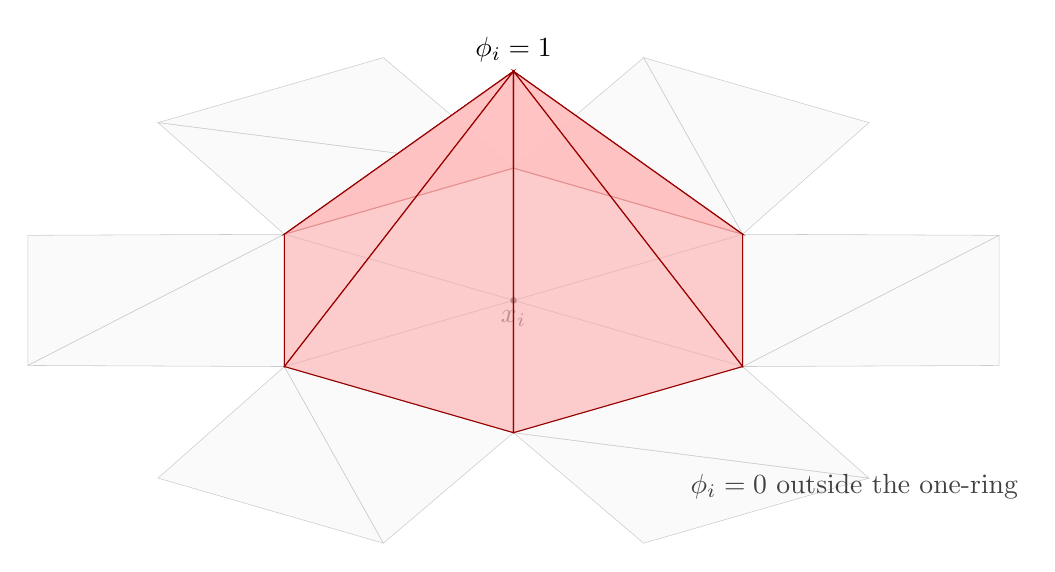
\begin{tikzpicture}[]
\filldraw[draw=gray!40, fill=gray!4, line width=0.2pt] (2.9098,-0.8400) -- (6.1665,-0.8262) -- (6.1665,0.8262) -- cycle;
\filldraw[draw=gray!40, fill=gray!4, line width=0.2pt] (2.9098,-0.8400) -- (6.1665,0.8262) -- (2.9098,0.8400) -- cycle;
\filldraw[draw=gray!40, fill=gray!4, line width=0.2pt] (2.9098,0.8400) -- (4.5142,2.2571) -- (1.6523,3.0832) -- cycle;
\filldraw[draw=gray!40, fill=gray!4, line width=0.2pt] (2.9098,0.8400) -- (1.6523,3.0832) -- (0.0000,1.6800) -- cycle;
\filldraw[draw=gray!40, fill=gray!4, line width=0.2pt] (0.0000,1.6800) -- (-1.6523,3.0832) -- (-4.5142,2.2571) -- cycle;
\filldraw[draw=gray!40, fill=gray!4, line width=0.2pt] (0.0000,1.6800) -- (-4.5142,2.2571) -- (-2.9098,0.8400) -- cycle;
\filldraw[draw=gray!40, fill=gray!4, line width=0.2pt] (-2.9098,0.8400) -- (-6.1665,0.8262) -- (-6.1665,-0.8262) -- cycle;
\filldraw[draw=gray!40, fill=gray!4, line width=0.2pt] (-2.9098,0.8400) -- (-6.1665,-0.8262) -- (-2.9098,-0.8400) -- cycle;
\filldraw[draw=gray!40, fill=gray!4, line width=0.2pt] (-2.9098,-0.8400) -- (-4.5142,-2.2571) -- (-1.6523,-3.0832) -- cycle;
\filldraw[draw=gray!40, fill=gray!4, line width=0.2pt] (-2.9098,-0.8400) -- (-1.6523,-3.0832) -- (0.0000,-1.6800) -- cycle;
\filldraw[draw=gray!40, fill=gray!4, line width=0.2pt] (0.0000,-1.6800) -- (1.6523,-3.0832) -- (4.5142,-2.2571) -- cycle;
\filldraw[draw=gray!40, fill=gray!4, line width=0.2pt] (0.0000,-1.6800) -- (4.5142,-2.2571) -- (2.9098,-0.8400) -- cycle;
\filldraw[draw=gray!60, fill=gray!8, line width=0.3pt] (0.0000,0.0000) -- (2.9098,-0.8400) -- (2.9098,0.8400) -- cycle;
\filldraw[draw=gray!60, fill=gray!8, line width=0.3pt] (0.0000,0.0000) -- (2.9098,0.8400) -- (0.0000,1.6800) -- cycle;
\filldraw[draw=gray!60, fill=gray!8, line width=0.3pt] (0.0000,0.0000) -- (0.0000,1.6800) -- (-2.9098,0.8400) -- cycle;
\filldraw[draw=gray!60, fill=gray!8, line width=0.3pt] (0.0000,0.0000) -- (-2.9098,0.8400) -- (-2.9098,-0.8400) -- cycle;
\filldraw[draw=gray!60, fill=gray!8, line width=0.3pt] (0.0000,0.0000) -- (-2.9098,-0.8400) -- (0.0000,-1.6800) -- cycle;
\filldraw[draw=gray!60, fill=gray!8, line width=0.3pt] (0.0000,0.0000) -- (0.0000,-1.6800) -- (2.9098,-0.8400) -- cycle;
\fill[fill=black] (0.0000,0.0000) circle (1.2pt) node[below] {$x_i$};
\filldraw[draw=red!60!black, fill=red!25, fill opacity=0.75, line width=0.4pt] (0.0000,2.9098) -- (0.0000,1.6800) -- (-2.9098,0.8400) -- cycle;
\filldraw[draw=red!60!black, fill=red!25, fill opacity=0.75, line width=0.4pt] (0.0000,2.9098) -- (2.9098,0.8400) -- (0.0000,1.6800) -- cycle;
\filldraw[draw=red!60!black, fill=red!25, fill opacity=0.75, line width=0.4pt] (0.0000,2.9098) -- (-2.9098,0.8400) -- (-2.9098,-0.8400) -- cycle;
\filldraw[draw=red!60!black, fill=red!25, fill opacity=0.75, line width=0.4pt] (0.0000,2.9098) -- (2.9098,-0.8400) -- (2.9098,0.8400) -- cycle;
\filldraw[draw=red!60!black, fill=red!25, fill opacity=0.75, line width=0.4pt] (0.0000,2.9098) -- (-2.9098,-0.8400) -- (0.0000,-1.6800) -- cycle;
\filldraw[draw=red!60!black, fill=red!25, fill opacity=0.75, line width=0.4pt] (0.0000,2.9098) -- (0.0000,-1.6800) -- (2.9098,-0.8400) -- cycle;
\node[above] at (0.0000,2.9098) {$\phi_i = 1$};
\node[right, gray!50!black] at (2.1253,-2.3594) {$\phi_i = 0$ outside the one-ring};
\end{tikzpicture}
}
\caption{The hat function $\phi_i$ of a vertex: linear on every face, $1$ at $x_i$, $0$ at all other vertices, and therefore zero outside the one-ring of $x_i$.}
\label{fig:hat}
\end{figure}

\subsection{Why the vector case needs a connection}

On a flat domain a vector unknown causes no difficulty. All the vertex vectors live in the same plane $\R^2$ and have coordinates in one common frame. The basis functions are the scalar hats times the two constant vectors of that frame, $\phi_i\, \varepsilon_k$, and a field is $\sum_i \phi_i\, u_i$, a combination of vectors that can be added because they lie in one plane. On a curved surface replaced by flat faces this fails, for a reason that is purely geometric.

The obvious vector analogue would be $U = \sum_i \phi_i\, (T_i u_i)$: interpolate the three vertex vectors of each face with the hat functions. But $T_i u_i$ lies in the tangent plane of vertex $i$, and the three vertices of a face have three different tangent planes, none of which is the plane of the face. The interpolated vector would not be tangent to the face, and its derivative would contain the bending of the surface rather than the turning of the field, which is precisely what the covariant derivative was designed to exclude. Before interpolating, the three vectors must be brought into one plane, the plane of the face. The rule that brings a vector from one tangent plane into another is parallel transport.
\begin{figure}[t]
\centering
\adjustbox{max width=\linewidth}{% generated by make_figures.py
\begin{tikzpicture}[]
\filldraw[draw=gray!70, fill=gray!10] (0.0000,0.0000) -- (5.2832,-0.3010) -- (4.3042,1.4797) -- cycle;
\filldraw[draw=blue!50, fill=blue!8, fill opacity=0.6] (-1.2651,-0.7209) -- (0.2591,-0.3449) -- (1.2651,0.7209) -- (-0.2591,0.3449) -- cycle;
\filldraw[draw=blue!50, fill=blue!8, fill opacity=0.6] (3.8878,-0.3577) -- (5.6555,-1.1369) -- (6.6785,-0.2444) -- (4.9108,0.5348) -- cycle;
\filldraw[draw=blue!50, fill=blue!8, fill opacity=0.6] (2.9155,1.5851) -- (4.7307,1.4339) -- (5.6929,1.3743) -- (3.8776,1.5254) -- cycle;
\draw[-{Stealth[length=2.2mm]}, thin, blue!60!black] (0.0000,0.0000) -- (-0.6820,1.2309);
\draw[-{Stealth[length=2.2mm]}, thin, blue!60!black] (5.2832,-0.3010) -- (5.4798,0.9034);
\draw[-{Stealth[length=2.2mm]}, thin, blue!60!black] (4.3042,1.4797) -- (4.4195,2.9471);
\draw[-{Stealth[length=2.2mm]}, very thick, red!70!black] (0.0000,0.0000) -- (1.6200,0.7296);
\draw[-{Stealth[length=2.2mm]}, very thick, red!70!black] (5.2832,-0.3010) -- (7.0056,-0.1520);
\draw[-{Stealth[length=2.2mm]}, very thick, red!70!black] (4.3042,1.4797) -- (5.4235,1.3789);
\draw[-{Stealth[length=2.2mm]}, very thick, green!50!black] (0.0000,0.0000) -- (1.8157,0.1307);
\draw[-{Stealth[length=2.2mm]}, very thick, green!50!black] (5.2832,-0.3010) -- (7.0080,0.0916);
\draw[-{Stealth[length=2.2mm]}, very thick, green!50!black] (4.3042,1.4797) -- (5.4286,1.1209);
\node[below] at (1.9056,-0.9693) {{\color{red!70!black}vertex vectors $T_i u_i$: three planes}};
\node[below] at (1.4456,-1.2677) {{\color{green!50!black}transported into the face: $T_f R_i^f u_i$}};
\end{tikzpicture}
}
\caption{Why vectors must be transported before they are interpolated. The vertex vectors $T_i u_i$ (red) lie in three different vertex planes (blue), none of which is the plane of the face; transported into the face, $T_f R_i^f u_i$ (green), they lie in one plane and can be combined.}
\label{fig:naive}
\end{figure}
So, on each face $f$, we interpolate the \emph{transported} vertex vectors. The vertex vector with coordinates $u_i$ in the vertex frame has, after transport into the face, the coordinates $R_i^f u_i$ in the face frame, by~(\ref{eqn:connection})~[\,$R_i^f = T_f^TQ_{i\to f}T_i$\,]; as a vector of $\R^3$ it is $T_f R_i^f u_i$. Interpolating these:
\begin{equation}
\label{eqn:trial}
U\big|_f = \sum_{i \in f} \phi_i\; T_f R_i^f u_i, \qquad \text{in face coordinates:} \quad T_f^T U\big|_f = \sum_{i \in f} \phi_i\, R_i^f u_i .
\end{equation}
The second form follows from the first. Multiply the first by $T_f^T$, with the sum in parentheses, and take the constant matrix inside:
\begin{align*}
T_f^T U\big|_f &= T_f^T \Big( \sum_{i\in f} \phi_i\; T_f R_i^f u_i \Big) \\
&= \sum_{i\in f} \phi_i\, (T_f^T T_f)\, R_i^f u_i \quad \text{(matrix product distributes; $\phi_i$ is a number)}\\
&= \sum_{i\in f} \phi_i\, R_i^f u_i \quad \text{($T_f^T T_f = I_2$, by~(\ref{eqn:frame}))}.
\end{align*}
Figure~\ref{fig:naive} shows the difference. Every term is a vector of the plane of the face, so the field is tangent to every face, and it is linear in the unknowns $u_i$.

\paragraph{The basis.} The space of such fields is spanned by $2n$ \emph{vector hat functions}, two per vertex:
\begin{equation}
\label{eqn:basis}
\Psi_{i,k}\big|_f = \phi_i\; T_f R_i^f \varepsilon_k, \qquad k = 1, 2,
\end{equation}
where $\varepsilon_1 = (1, 0)$ and $\varepsilon_2 = (0, 1)$. In words: the frame vector $k$ of vertex $i$, transported into each incident face, and faded out by the scalar hat. Then $U = \sum_{i,k} u_{i,k} \Psi_{i,k}$, with the unknowns~(\ref{eqn:dofs})~[\,$\mathrm u = (u_{1,1}, u_{1,2}, \ldots, u_{n,2})$\,] as coefficients. To check it on one face, take the two basis functions of vertex $i$, substitute~(\ref{eqn:basis}), and take the common factors out:
\begin{align*}
\sum_{k} u_{i,k}\Psi_{i,k}\big|_f &= \sum_k u_{i,k}\, \big(\phi_i\, T_f R_i^f \varepsilon_k\big) \\
&= \phi_i\, T_f R_i^f \Big(\sum_k u_{i,k}\varepsilon_k\Big) \quad \text{($\phi_i T_fR_i^f$ does not depend on $k$)}\\
&= \phi_i\, T_f R_i^f u_i \quad \text{($u_{i,1}(1,0) + u_{i,2}(0,1) = u_i$)} .
\end{align*}
Summing over the vertices $i$ of $f$ gives~(\ref{eqn:trial})~[\,$U|_f = \sum_{i\in f}\phi_i\, T_fR_i^f u_i$\,]. At vertex $i$ itself, $\phi_i = 1$ and the other hats vanish, so the field takes, in each incident face, the transported value $T_f R_i^f u_i$: the vertex vector seen from that face. As a vector of $\R^3$ the field is not continuous across the edges, since two neighboring faces have different planes. Continuity must be understood after unfolding one face onto the other, and Section~\ref{section:r1_conformity} shows that in this sense it holds, approximately. Inside each face it is a smooth tangent field, whose covariant derivative we can compute.

\subsection{How the differential geometry fits into the finite element machinery}
\label{section:r1_geometry_fem}

It helps to list exactly where the geometry of Sections~\ref{section:geometry} and~\ref{section:transport} enters the machinery, and where it does not. Go through the mesh piece by piece.
\begin{enumerate}
\item \emph{Inside a face} nothing is curved. The face is a flat triangle with one tangent plane and a constant frame $T_f$, so $D_X T_f = 0$ and the connection form $\omega(X) = T_f^T D_X T_f$ of~(\ref{eqn:covariant_frame})~[\,$T^T\nabla_X U = X\cdot\nabla u + \omega(X)\, u$\,] vanishes: the covariant derivative is the ordinary derivative of the face coordinates. Inside each face the method is the planar finite element method for a field with two components.
\item \emph{At a vertex} there is no tangent plane. Several faces with several planes meet there, and the method needs one plane, because the unknown vector lives at the vertex. The vertex normal supplies it; this is a modelling choice, made with the positions of the vertices in space.
\item \emph{Between a vertex and a face} the two planes differ, and a vertex vector cannot be used in the face until it has been brought into the plane of the face. This is the one place where the curvature of the surface enters the finite element space: the discrete connection $R_i^f$, applied to the vertex coordinates \emph{before} the hat function is differentiated. In the continuous theory, the covariant derivative is the ordinary derivative taken after all the vectors have been transported into one common plane (Section~\ref{section:transport}). On a face, that common plane is the plane of the face, and $R_i^f$ is the transport. The matrices $R_i^f$ take over the role that the connection form $\omega$ plays in the smooth formula, as Section~\ref{section:r1_basis_derivative} shows.
\item \emph{Across an edge} two faces meet at an angle. A vector of one face and a vector of the other can be compared only after one face has been unfolded onto the plane of the other, rotating it about the shared edge (Figure~\ref{fig:unfold}); that unfolding is the parallel transport of the polyhedral surface. Whether the discrete fields are continuous in this sense is the conformity question of Stage 2, answered in the next subsection.
\item \emph{Around a vertex} the transports from face to face compose to a rotation that is not the identity: the holonomy of Example~\ref{ex:holonomy}, the discrete Gaussian curvature. So no discrete field can be parallel everywhere, the energy $\int|\nabla U|^2$ cannot be made zero, and the curvature reaches the result of the method through the rotations.
\end{enumerate}
So the finite element machinery itself is unchanged, stage by stage. What the geometry changes is the basis functions of Stage 5, and through them, in Stage 7, the element matrices.

\paragraph{What is extrinsic in this part.} A quantity is \emph{intrinsic} if a creature living on the surface could compute it from measurements on the surface (lengths, angles, areas), and \emph{extrinsic} if it needs the position of the surface in space. Part~\ref{part:matrix} works extrinsically throughout: it stores vectors of $\R^3$ and uses the normals. Table~\ref{tab:r1_extrinsic} says what each ingredient is; Part~\ref{part:ga} examines this more closely, and Part~\ref{part:intrinsic} rebuilds the method from edge lengths alone.
\begin{table}[t]
\centering
\caption{The ingredients of the finite element space of this part: which are extrinsic (they need the position of the surface in space) and which are intrinsic (they could be measured on the surface).}
\label{tab:r1_extrinsic}
\footnotesize
\setlength{\tabcolsep}{3pt}
\begin{tabular}{>{\raggedright\arraybackslash}p{0.36\linewidth} >{\raggedright\arraybackslash}p{0.56\linewidth}}
\toprule
ingredient & extrinsic or intrinsic \\
\midrule
face normal $n_f$, projection $I - nn^T$ & extrinsic: they describe the position of the plane in space \\
vertex normal $n_i$, vertex plane & extrinsic, and a modelling choice: the polyhedral surface has no plane at a vertex \\
smallest rotation $Q_{i\to f}$, hence $R_i^f$ & extrinsic: defined by the two normals in space \\
covariant derivative inside a face & intrinsic: the normal part has been discarded \\
area $A_f$, products $g_a^f\cdot g_b^f$ & intrinsic: by the cotangent formula (Proposition~\ref{prop:cotangent}), they depend only on the angles and the area of the triangle \\
transports $(R_a^f)^TR_b^f$ in the stiffness & extrinsic as computed; they approximate the intrinsic transport on fine meshes (Remark on curvature, Section~\ref{section:transport}) \\
\bottomrule
\end{tabular}
\end{table}
The scalar part of the method is therefore intrinsic, even though the code computes it from positions in space through the $3\times 2$ matrix $B$ of Section~\ref{section:gradients}; only the transports depend on the embedding.

\subsection{Is the space conforming?}
\label{section:r1_conformity}

Stage 2 asked for continuity across the edges, understood after unfolding. Take an edge $ij$ shared by the faces $f$ and $g$, and look at the vertex $i$ first. Seen from face $f$, the field at $x_i$ is $T_f R_i^f u_i$; seen from $g$, it is $T_g R_i^g u_i$. The first can be written without the face frame. Substitute $R_i^f = T_f^TQ_{i\to f}T_i$ in parentheses and regroup:
\begin{align*}
T_f R_i^f u_i &= T_f\big(T_f^T Q_{i\to f}T_i\big) u_i \\
&= (T_f T_f^T)\, (Q_{i\to f}T_i u_i) \quad \text{(associativity)}\\
&= (I - n_fn_f^T)\, (Q_{i\to f}T_i u_i) \quad \text{($TT^T = I - nn^T$, by~(\ref{eqn:frame}))}\\
&= Q_{i\to f}T_i u_i \quad \text{($Q_{i\to f}T_iu_i$ is orthogonal to $n_f$)} .
\end{align*}
The last step holds because the columns of $Q_{i\to f}T_i$ lie in the plane of $f$ (Proposition~\ref{prop:connection_rotation}), so the projection does not change them. Likewise $T_gR_i^gu_i = Q_{i\to g}T_iu_i$. Unfold $g$ onto $f$ with the rotation about the shared edge, which is the smallest rotation $Q_{g\to f}$ from $n_g$ to $n_f$ (Section~\ref{section:transport}). The two values agree, for every $u_i$, when
\begin{equation*}
Q_{g\to f}\, Q_{i\to g}\, T_i = Q_{i\to f}\, T_i :
\end{equation*}
going from the vertex plane into $g$ and then across the edge into $f$ must give the same as going directly from the vertex plane into $f$. Both sides take $n_i$ to $n_f$, so they differ at most by a rotation about $n_i$, a rotation of the vertex plane by some angle. That angle is the holonomy of the closed path $n_i \to n_g \to n_f \to n_i$ traced by the normals on the unit sphere. The reason is that a smallest rotation turns a tangent plane of the unit sphere exactly as parallel transport along the great circle arc between the two normals does. By Example~\ref{ex:holonomy} (the sphere has curvature $1$, and holonomy is enclosed area) the angle is the area of the small spherical triangle with vertices $n_i$, $n_g$, $n_f$. Two consequences follow.
\begin{itemize}
\item It is zero when the three normals lie on one great circle. This happens at every vertex whose faces are folded along parallel lines (the folds of a prism), where all the face normals, and therefore their average $n_i$, are orthogonal to the fold direction. There the space is exactly conforming.
\item In general it is of second order in the angles between the normals. For instance, with $n_i = (0, 0, 1)$ and the two face normals tilted by $\alpha = 0.1$ radians ($5.7^\circ$) about the $x$ and the $y$ axis, the mismatch is $0.0050$ radians ($0.29^\circ$), close to the area $\alpha^2/2$ of the triangle; with $\alpha = 0.05$ it is a quarter of that, $0.07^\circ$. On a smooth surface sampled with spacing $h$ the angles between neighboring normals are of order $h$, so the mismatch is of order $h^2$.
\end{itemize}
Along the edge, each side of the field is the linear interpolation, with the hats of $i$ and $j$, of its two end values, and the unfolding is a linear map. So the mismatch along the edge is the linear interpolation of the mismatches at its two ends, and the edge matches wherever both of its ends do. The space of this part is therefore conforming exactly on meshes of parallel folds and approximately on curved meshes, with a mismatch that shrinks quickly under refinement. The method ignores the mismatch: its element integrals are computed face by face, as for a conforming space. Part~\ref{part:intrinsic} shows what happens when the mismatch is not small, on a sheet folded in four directions at every vertex, where the rotated faces no longer fit edge to edge.

\subsection{The covariant derivative of a basis function}
\label{section:r1_basis_derivative}

The weak form needs $\nabla U$ for $U$ in the space just built; this is the last property of the space, and the one that Stage 7 will integrate. We compute it on one face, where everything is simple. Inside a face, the surface is a plane and the face frame $T_f$ is constant, so $D_X T_f = 0$ and the connection form $\omega(X) = T_f^T D_X T_f$ vanishes. Then~(\ref{eqn:covariant_frame}), with $\omega = 0$, says that the covariant derivative is the ordinary derivative of the face coordinates:
\begin{equation*}
T^T \nabla_X U = X\cdot\nabla u + \omega(X)\, u \quad\Longrightarrow\quad T_f^T\nabla_X U = X\cdot\nabla(T_f^T U) ,
\end{equation*}
where $u = T_f^TU$ are the face coordinates of the field and $X\cdot\nabla$ is the directional derivative along $X$. Now substitute the face coordinates of the discrete field, (\ref{eqn:trial})~[\,$T_f^T U|_f = \sum_{i\in f} \phi_i\, R_i^f u_i$\,], in parentheses, and take one operation per line:
\begin{align*}
T_f^T\nabla_X U\big|_f &= X\cdot\nabla \Big(\sum_{i\in f} \phi_i\, R_i^f u_i\Big) \\
&= \sum_{i\in f} X\cdot\nabla\big(\phi_i\, R_i^f u_i\big) \quad \text{(derivative of a sum)}\\
&= \sum_{i\in f} (X\cdot\nabla\phi_i)\, R_i^f u_i \quad \text{($R_i^fu_i$ is constant on the face)} .
\end{align*}
The last line uses that the derivative of a function times a constant vector is the derivative of the function times the vector, $X(\phi\, c) = X(\phi)\, c$. Write $g_i^f = T_f^T \nabla \phi_i \in \R^2$ for the gradient of the hat function in the coordinates of the face. It is a constant vector on the face, since $\phi_i$ is linear there (Section~\ref{section:transport}), and Section~\ref{section:gradients} computes it. If $x = T_f^T X$ are the face coordinates of the direction $X$, then
\begin{equation*}
X\cdot\nabla\phi_i = (T_f x)\cdot\nabla\phi_i = x\cdot (T_f^T\nabla\phi_i) = x \cdot g_i^f = (g_i^f)^T x .
\end{equation*}
Substituting this into the last line above, in parentheses, and taking the common vector $x$ out to the right:
\begin{align*}
&\sum_{i\in f} (X\cdot\nabla\phi_i)\, R_i^f u_i \\
&\quad= \sum_{i\in f} \big((g_i^f)^T x\big)\, R_i^f u_i \\
&\quad= \sum_{i\in f} (R_i^f u_i)\big((g_i^f)^T x\big) \quad \text{(a number commutes with a vector)}\\
&\quad= \sum_{i\in f} \big((R_i^f u_i)(g_i^f)^T\big)\, x \quad \text{(associativity: column, row, column)}\\
&\quad= \Big(\sum_{i\in f} (R_i^f u_i)(g_i^f)^T\Big)\, x \quad \text{(distributivity)} .
\end{align*}
The $2\times 2$ matrix in brackets, applied to the coordinates of the direction, gives the coordinates of the derivative, which is what the matrix of $\nabla U$ is. We have found both forms of the covariant derivative of the discrete field:
\begin{equation}
\label{eqn:grad_trial}
T_f^T \nabla_X U\big|_f = \sum_{i \in f} (X \cdot \nabla \phi_i)\, R_i^f u_i, \qquad T_f^T \nabla U\big|_f = \sum_{i \in f} (R_i^f u_i)\, (g_i^f)^T .
\end{equation}
The total covariant derivative is a sum of rank-one $2 \times 2$ matrices, each a column times a row: the transported vertex vector times the gradient of its hat. For a single basis function, with $u_i$ replaced by $\varepsilon_k$ and the other vertices set to zero, $\nabla \Psi_{i,k}$ has the matrix $(R_i^f \varepsilon_k)(g_i^f)^T$; in tensor notation, $\nabla \Psi_{i,k} = (R_i^f \varepsilon_k) \otimes g_i^f$.

\paragraph{Where the connection went.} Compare~(\ref{eqn:grad_trial}) with the continuous formula~(\ref{eqn:covariant_frame})~[\,$T^T\nabla_X U = X\cdot\nabla u + \omega(X)\,u$\,]. In the continuous setting, the turning of the frame appears as the term $\omega(X)\, u$ inside the derivative. In the discrete field there is no such term: inside every face the frame is constant and $\omega = 0$. The turning has not disappeared; it has been moved out of the derivative and into the matrices $R_i^f$, which are applied \emph{before} differentiating. Each vertex vector is first expressed in the frame of the face, and only then are the hats differentiated. The rotation $R_i^f$ plays the role of the connection form accumulated along the short way from the vertex into the face, which, by Section~\ref{section:transport}, is what parallel transport does to coordinates. This is why the code never differentiates a frame: the only trace of the connection is the rotations computed by \code{Rvf}.

\paragraph{What Stage 5 produced.} The discrete space
\begin{equation*}
V_h = \Big\{ \sum_{i,k} u_{i,k}\, \Psi_{i,k} \Big\}, \qquad \Psi_{i,k}\big|_f = \phi_i\; T_f R_i^f \varepsilon_k ,
\end{equation*}
of dimension $2n$, spanned by the vector hat functions~(\ref{eqn:basis}). Each basis function is tangent to every face, vanishes outside the one-ring of its vertex, and has on each face the constant covariant derivative $(R_i^f\varepsilon_k)(g_i^f)^T$ of~(\ref{eqn:grad_trial}). The geometry of the surface enters only through the rotations $R_i^f$, and the space is conforming exactly on meshes of parallel folds and approximately in general.

%%% ----------------------------------------------------------------------
\section{Stage 6. The Discrete Solution and the Test Functions}
\label{section:r1_discrete}

\paragraph{What we want.} Finitely many equations for finitely many numbers. Stage 2 wrote the target, the Galerkin problem~(\ref{eqn:r1_galerkin_abstract}) again:
\begin{equation*}
\text{find } U_h \in V_h \text{ such that } a(U_h, V_h) = l(V_h) \text{ for every } V_h \in V_h , \tag{\ref{eqn:r1_galerkin_abstract}}
\end{equation*}
with the forms $a$ and $l$ of~(\ref{eqn:r1_forms}) again,
\begin{equation*}
a(U, V) = \int_\Omega U\cdot V\, dA + \Delta t \int_\Omega \nabla U : \nabla V\, dA, \qquad l(V) = \int_\Omega U^0\cdot V\, dA . \tag{\ref{eqn:r1_forms}}
\end{equation*}
Two moves turn it into a linear system: write the unknown with the basis, and test with the basis.

\paragraph{The discrete solution.} Every field of $V_h$ is a combination of the basis functions, so the unknown is
\begin{equation}
\label{eqn:r1_trial_sum}
U_h = \sum_{j,l} u_{j,l}\, \Psi_{j,l} ,
\end{equation}
and the $2n$ coefficients $u_{j,l}$, the coordinates~(\ref{eqn:dofs}) of the vertex vectors, are the unknowns. We use the letters $j, l$ for the unknown and keep $i, k$ for the test function. On a face this is the interpolation of the transported vertex vectors, (\ref{eqn:trial}) again:
\begin{equation*}
U\big|_f = \sum_{i \in f} \phi_i\; T_f R_i^f u_i . \tag{\ref{eqn:trial}}
\end{equation*}
From now on we write $U$ for $U_h$, as the code does.

\paragraph{The test functions.} Asking the equation for every $V_h \in V_h$ is the same as asking it for the $2n$ basis functions. One direction is clear, since the basis functions belong to $V_h$. Conversely, suppose that $a(U, \Psi_{i,k}) = l(\Psi_{i,k})$ for every $(i, k)$, and take any $V_h = \sum_{i,k} v_{i,k}\Psi_{i,k}$. Multiply the equation $(i, k)$ by the number $v_{i,k}$ and add all of them. Both forms are linear in the test field, so the numbers and the sum go inside:
\begin{align*}
\sum_{i,k} v_{i,k}\, a(U, \Psi_{i,k}) &= \sum_{i,k} v_{i,k}\, l(\Psi_{i,k}) \\
a\Big(U, \sum_{i,k} v_{i,k}\Psi_{i,k}\Big) &= l\Big(\sum_{i,k} v_{i,k}\Psi_{i,k}\Big) \quad \text{(linearity of $a$ and $l$ in $V$)}\\
a(U, V_h) &= l(V_h) .
\end{align*}
So the test fields are $V = \Psi_{i,k}$, one per unknown: the \emph{Galerkin} choice, in which test and trial spaces are the same.

\paragraph{Substituting.} Recall the weak form~(\ref{eqn:weak}):
\begin{equation*}
\int_\Omega U \cdot V\, dA + \Delta t \int_\Omega \nabla U : \nabla V\, dA = \int_\Omega U^0 \cdot V\, dA . \tag{\ref{eqn:weak}}
\end{equation*}
And recall the discrete solution~(\ref{eqn:r1_trial_sum})~[\,$U = \sum_{j,l} u_{j,l}\Psi_{j,l}$\,]. Substitute the sum for $U$ and the basis function $\Psi_{i,k}$ for $V$, each in parentheses; the data $U^0$ stays as it is for the moment:
\begin{equation*}
\begin{split}
\int_\Omega \Big(\sum_{j,l} u_{j,l}\Psi_{j,l}\Big) \cdot \Psi_{i,k}\, dA &+ \Delta t \int_\Omega \nabla\Big(\sum_{j,l} u_{j,l}\Psi_{j,l}\Big) : \nabla \Psi_{i,k}\, dA \\
&= \int_\Omega U^0 \cdot \Psi_{i,k}\, dA .
\end{split}
\end{equation*}
Now we move the sums and the numbers $u_{j,l}$ out, one operation per line. The first term:
\begin{align*}
&\int_\Omega \Big(\sum_{j,l} u_{j,l}\Psi_{j,l}\Big) \cdot \Psi_{i,k}\, dA \\
&\quad= \int_\Omega \sum_{j,l} \big(u_{j,l}\Psi_{j,l}\big) \cdot \Psi_{i,k}\, dA \quad \text{($\cdot$ distributes over the sum)}\\
&\quad= \int_\Omega \sum_{j,l} u_{j,l}\, \big(\Psi_{j,l} \cdot \Psi_{i,k}\big)\, dA \quad \text{(a number comes out of $\cdot$)}\\
&\quad= \sum_{j,l} \int_\Omega u_{j,l}\, \Psi_{j,l} \cdot \Psi_{i,k}\, dA \quad \text{(integral of a finite sum)}\\
&\quad= \sum_{j,l} u_{j,l} \int_\Omega \Psi_{j,l} \cdot \Psi_{i,k}\, dA \quad \text{(a constant comes out of $\textstyle\int$)} .
\end{align*}
The second term needs one more step at the start: the covariant derivative is linear, $\nabla(V + W) = \nabla V + \nabla W$ and $\nabla(cV) = c\,\nabla V$ for a number $c$, because it is the tangent part of a directional derivative and both taking a derivative and taking the tangent part are linear. Then:
\begin{align*}
&\int_\Omega \nabla\Big(\sum_{j,l} u_{j,l}\Psi_{j,l}\Big) : \nabla \Psi_{i,k}\, dA \\
&\quad= \int_\Omega \Big(\sum_{j,l} u_{j,l}\,\nabla\Psi_{j,l}\Big) : \nabla \Psi_{i,k}\, dA \quad \text{($\nabla$ is linear)}\\
&\quad= \int_\Omega \sum_{j,l} u_{j,l}\, \big(\nabla\Psi_{j,l} : \nabla \Psi_{i,k}\big)\, dA \quad \text{($:$ is linear in its first factor)}\\
&\quad= \sum_{j,l} u_{j,l} \int_\Omega \nabla\Psi_{j,l} : \nabla \Psi_{i,k}\, dA \quad \text{(sum and constant out of $\textstyle\int$)} .
\end{align*}
Put the two results back into the substituted equation, the second multiplied by $\Delta t$:
\begin{equation*}
\sum_{j,l} u_{j,l} \int_\Omega \Psi_{j,l} \cdot \Psi_{i,k}\, dA + \Delta t \sum_{j,l} u_{j,l}\int_\Omega \nabla \Psi_{j,l} : \nabla \Psi_{i,k}\, dA = \int_\Omega U^0 \cdot \Psi_{i,k}\, dA .
\end{equation*}
The two sums on the left run over the same indices $(j, l)$, so they merge into one sum, and in each of its terms the common factor $u_{j,l}$ is taken out to the right. We have one equation per test function, $2n$ linear equations in the $2n$ unknowns:
\begin{equation}
\label{eqn:galerkin}
\sum_{j,l} \Big( \int_\Omega \Psi_{j,l} \cdot \Psi_{i,k}\, dA + \Delta t \int_\Omega \nabla \Psi_{j,l} : \nabla \Psi_{i,k}\, dA \Big)\, u_{j,l} = \int_\Omega U^0 \cdot \Psi_{i,k}\, dA ,
\end{equation}
that is, $\sum_{j,l} a(\Psi_{j,l}, \Psi_{i,k})\, u_{j,l} = l(\Psi_{i,k})$. The bracket on the left is the number $a(\Psi_{j,l}, \Psi_{i,k})$: it is the coefficient of the unknown $u_{j,l}$ in the equation of the test function $\Psi_{i,k}$.

\paragraph{The right side with the interpolated data.} The right side of~(\ref{eqn:galerkin}) is an integral of the data. To write it with numbers at the vertices, like the left side, we replace $U^0$ by its interpolant in the same space,
\begin{equation*}
U^0 = \sum_{j,l} u^0_{j,l}\,\Psi_{j,l} ,
\end{equation*}
with the coordinates $u^0_{j,l}$ of the data at the vertices, $\mathrm u^0 = (u^0_{1,1}, u^0_{1,2}, \ldots, u^0_{n,2})$. Substituting it, in parentheses, into the right side of~(\ref{eqn:galerkin}) and taking the same four steps as for the first term of the left side:
\begin{align*}
&\int_\Omega U^0 \cdot \Psi_{i,k}\, dA \\
&\quad= \int_\Omega \Big(\sum_{j,l} u^0_{j,l}\Psi_{j,l}\Big) \cdot \Psi_{i,k}\, dA \\
&\quad= \int_\Omega \sum_{j,l} u^0_{j,l}\, \big(\Psi_{j,l} \cdot \Psi_{i,k}\big)\, dA \quad \text{($\cdot$ distributes; the number comes out)}\\
&\quad= \sum_{j,l} u^0_{j,l} \int_\Omega \Psi_{j,l} \cdot \Psi_{i,k}\, dA \quad \text{(sum and constant out of $\textstyle\int$)} .
\end{align*}
So, with the interpolated data, equation $(i, k)$ of~(\ref{eqn:galerkin}) becomes
\begin{equation*}
\begin{split}
\sum_{j,l} \Big( \int_\Omega \Psi_{j,l} \cdot \Psi_{i,k}\, dA &+ \Delta t \int_\Omega \nabla \Psi_{j,l} : \nabla \Psi_{i,k}\, dA \Big)\, u_{j,l} \\
&= \sum_{j,l} \Big(\int_\Omega \Psi_{j,l}\cdot \Psi_{i,k}\, dA\Big)\, u^0_{j,l} .
\end{split}
\end{equation*}
(In the code the data is zero away from the source vertex, and the two equations of the source vertex are replaced by its prescribed value, Section~\ref{section:solve}.)

\paragraph{The matrix form.} Give names to the two integrals. For each pair of indices, a row index $(i, k)$ and a column index $(j, l)$, let
\begin{equation*}
\mathrm M_{(i,k),(j,l)} = \int_\Omega \Psi_{j,l} \cdot \Psi_{i,k}\, dA, \qquad \mathrm L_{(i,k),(j,l)} = \int_\Omega \nabla \Psi_{j,l} : \nabla \Psi_{i,k}\, dA .
\end{equation*}
Substituting these names into the last equation, equation $(i, k)$ reads
\begin{equation*}
\sum_{j,l} \big( \mathrm M_{(i,k),(j,l)} + \Delta t\, \mathrm L_{(i,k),(j,l)}\big)\, u_{j,l} = \sum_{j,l} \mathrm M_{(i,k),(j,l)}\, u^0_{j,l} .
\end{equation*}
A sum over the column index of a matrix entry times the entry of a vector is one entry of the product of the matrix with the vector: the left side is entry $(i, k)$ of $(\mathrm M + \Delta t\,\mathrm L)\,\mathrm u$, and the right side is entry $(i, k)$ of $\mathrm M\,\mathrm u^0$. All the $2n$ equations together are
\begin{equation}
\label{eqn:linear_system}
(\mathrm M + \Delta t\, \mathrm L)\, \mathrm u = \mathrm M\, \mathrm u^0 ,
\end{equation}
with the \emph{mass matrix} $\mathrm M$ and the \emph{stiffness matrix} $\mathrm L$, both $2n \times 2n$. Grouping the two rows of vertex $i$ and the two columns of vertex $j$, both are made of $2 \times 2$ blocks, one per pair of vertices $(i, j)$:
\begin{equation}
\label{eqn:global_blocks}
\mathrm M_{ij} = \Big[ \int_\Omega \Psi_{j,l} \cdot \Psi_{i,k}\, dA \Big]_{k,l}, \qquad \mathrm L_{ij} = \Big[ \int_\Omega \nabla \Psi_{j,l} : \nabla \Psi_{i,k}\, dA \Big]_{k,l}.
\end{equation}
So the row index belongs to the test function and the column index to the unknown.

\paragraph{The Galerkin equations as a minimization.} The weak form was the condition that the energy of Stage 3 be stationary, (\ref{eqn:weak_energy}) again:
\begin{equation*}
J(U) = \frac12 \int_\Omega |U|^2\, dA + \frac{\Delta t}{2} \int_\Omega |\nabla U|^2\, dA - \int_\Omega U^0 \cdot U\, dA . \tag{\ref{eqn:weak_energy}}
\end{equation*}
The Galerkin equations have the same reading in the finite space. Substitute $U = \sum_{i,k} u_{i,k}\Psi_{i,k}$ in the first term, writing $|U|^2 = U\cdot U$ and using the letters $(i, k)$ for one factor and $(j, l)$ for the other:
\begin{align*}
&\int_\Omega |U|^2\, dA \\
&\quad= \int_\Omega \Big(\sum_{i,k} u_{i,k}\Psi_{i,k}\Big)\cdot\Big(\sum_{j,l} u_{j,l}\Psi_{j,l}\Big)\, dA \\
&\quad= \int_\Omega \sum_{i,k}\sum_{j,l} u_{i,k}\,u_{j,l}\, \Psi_{i,k}\cdot\Psi_{j,l}\, dA \quad \text{($\cdot$ distributes over both sums)}\\
&\quad= \sum_{i,k}\sum_{j,l} u_{i,k}\Big(\int_\Omega \Psi_{j,l}\cdot\Psi_{i,k}\, dA\Big) u_{j,l} \quad \text{(sums and numbers out of $\textstyle\int$)}\\
&\quad= \sum_{i,k}\sum_{j,l} u_{i,k}\, \mathrm M_{(i,k),(j,l)}\, u_{j,l} = \mathrm u^T \mathrm M\, \mathrm u \quad \text{(definition of $\mathrm M$)} .
\end{align*}
The same four lines with $\nabla$ (which is linear) and $:$ in place of $\cdot$ give $\int_\Omega |\nabla U|^2\, dA = \mathrm u^T\mathrm L\,\mathrm u$, and with the sum for $U^0$ in the first factor they give $\int_\Omega U^0\cdot U\, dA = \mathrm u^T\mathrm M\,\mathrm u^0$ (here we use that $\mathrm M$ is symmetric, which holds because $\Psi_{j,l}\cdot\Psi_{i,k} = \Psi_{i,k}\cdot\Psi_{j,l}$). Substituting these three expressions into the three terms of~(\ref{eqn:weak_energy}):
\begin{align*}
J(\mathrm u) &= \tfrac12\, \big(\mathrm u^T \mathrm M\, \mathrm u\big) + \tfrac{\Delta t}{2}\, \big(\mathrm u^T \mathrm L\, \mathrm u\big) - \big(\mathrm u^T \mathrm M\, \mathrm u^0\big) \\
&= \tfrac12\, \mathrm u^T (\mathrm M + \Delta t\,\mathrm L)\, \mathrm u - \mathrm u^T \mathrm M\, \mathrm u^0 \quad \text{(the first two share $\tfrac12\mathrm u^T\cdots\mathrm u$)} .
\end{align*}
On the finite space $J$ is a function of the $2n$ numbers $\mathrm u$. Its minimum is where its partial derivatives vanish. For a symmetric matrix $\mathrm A$ and a vector $\mathrm c$, write the two kinds of terms entry by entry and differentiate with respect to one entry $u_p$; the product rule hits each of the two factors $u_q$ and $u_r$ once:
\begin{align*}
\frac{\partial}{\partial u_p}\Big(\frac12\sum_{q}\sum_{r} u_q\, \mathrm A_{qr}\, u_r\Big) &= \frac12\sum_{r} \mathrm A_{pr}\, u_r + \frac12\sum_{q} u_q\, \mathrm A_{qp} \\
&= \frac12 (\mathrm A\mathrm u)_p + \frac12 (\mathrm A\mathrm u)_p = (\mathrm A\mathrm u)_p \quad \text{($\mathrm A_{qp} = \mathrm A_{pq}$)},\\
\frac{\partial}{\partial u_p}\Big(\sum_q u_q\, \mathrm c_q\Big) &= \mathrm c_p .
\end{align*}
With $\mathrm A = \mathrm M + \Delta t\,\mathrm L$ and $\mathrm c = \mathrm M\,\mathrm u^0$, the gradient of $J$ is $(\mathrm M + \Delta t\,\mathrm L)\,\mathrm u - \mathrm M\,\mathrm u^0$, and setting it to zero gives~(\ref{eqn:linear_system})~[\,$(\mathrm M + \Delta t\,\mathrm L)\,\mathrm u = \mathrm M\,\mathrm u^0$\,]. The Galerkin solution is the minimizer of the same energy over the finite space: the best piecewise linear tangent field in the sense of $J$. Testing with the same functions as the unknowns is what makes the matrix of the system symmetric, as the matrix of second derivatives of an energy must be.

\paragraph{Sparsity.} Each integral is a sum over faces, and a face contributes to the block $(i, j)$ only if it contains both $i$ and $j$, because the hats vanish elsewhere. So the matrices are sparse, with a nonzero block for each vertex and for each pair of vertices joined by an edge: about seven blocks per row on a typical mesh, out of $n$. And they can be computed face by face, which is the next stage.

\paragraph{What Stage 6 produced.} The linear system~(\ref{eqn:linear_system})~[\,$(\mathrm M + \Delta t\,\mathrm L)\,\mathrm u = \mathrm M\,\mathrm u^0$\,], symmetric, sparse and positive definite, whose matrices are made of the integrals~(\ref{eqn:global_blocks}) of products of basis functions and of their covariant derivatives. By C\'ea's lemma of Stage 2 its solution is the best field of $V_h$ in the energy norm, and by Stage 3 it is the minimizer of $J$ over $V_h$. What is still missing is the value of every integral; that is Stage 7.

%%% ----------------------------------------------------------------------
\section{Stage 7. The Element Integrals}
\label{section:r1_element_integrals}

\paragraph{What we want.} The numbers in the matrices of Stage 6, (\ref{eqn:global_blocks}) again:
\begin{equation*}
\mathrm M_{ij} = \Big[ \int_\Omega \Psi_{j,l} \cdot \Psi_{i,k}\, dA \Big]_{k,l}, \qquad \mathrm L_{ij} = \Big[ \int_\Omega \nabla \Psi_{j,l} : \nabla \Psi_{i,k}\, dA \Big]_{k,l}. \tag{\ref{eqn:global_blocks}}
\end{equation*}
Every integral over the mesh is the sum of the integrals over its faces, and on one face only the basis functions of its three vertices are nonzero. So the work splits into small pieces, one per face: the \emph{element integrals}. This stage computes them in three steps. Here we substitute the covariant derivatives of the basis functions into the integrand of $\mathrm L_{ij}$ and find the stiffness block of a face in terms of the hat gradients $g_i^f$. Section~\ref{section:gradients} computes those gradients on a reference triangle, with the chain rule and the affine map to the face. Section~\ref{section:element} collects the blocks of a face into its element matrices, stiffness and mass, with the code that computes them.

\paragraph{The stiffness block of a face.} Fix a face $f$ that contains the two vertices $i$ and $j$. Its contribution to the block $\mathrm L_{ij}$ is the $2\times 2$ matrix of the integrals over $f$ alone,
\begin{equation*}
\mathrm L^f_{ij} = \Big[ \int_f \nabla \Psi_{j,l} : \nabla \Psi_{i,k}\, dA \Big]_{k,l} .
\end{equation*}
On the face, the covariant derivative of a basis function is~(\ref{eqn:grad_trial})~[\,$T_f^T \nabla U|_f = \sum_{i \in f} (R_i^f u_i)\, (g_i^f)^T$\,] with $u_i$ replaced by $\varepsilon_k$ and the coordinates of the other two vertices set to zero (Section~\ref{section:r1_basis_derivative}):
\begin{equation*}
T_f^T\nabla \Psi_{i,k}\big|_f = (R_i^f\varepsilon_k)(g_i^f)^T, \qquad T_f^T\nabla \Psi_{j,l}\big|_f = (R_j^f\varepsilon_l)(g_j^f)^T ,
\end{equation*}
two rank-one $2\times 2$ matrices, each a column times a row. The inner product $:$ of two covariant derivatives can be computed with their matrices in the face frame, because the frame is orthonormal (Section~\ref{section:pde}), and it is the sum of the products of the entries, (\ref{eqn:dirichlet})~[\,$A : B = \sum_{p,q} A_{pq}B_{pq}$\,].

\paragraph{The inner product of two rank-one matrices.} Take four vectors $a, b, c, d$ of $\R^2$. The entry $(p, q)$ of $a b^T$ is $a_p b_q$, and that of $c d^T$ is $c_p d_q$. Then
\begin{align*}
(a b^T) : (c d^T) &= \sum_{p}\sum_{q} (a_p b_q)(c_p d_q) \quad \text{(definition of $:$)}\\
&= \sum_{p}\sum_{q} (a_p c_p)(b_q d_q) \quad \text{(reorder the four numbers)}\\
&= \Big(\sum_{p} a_p c_p\Big)\Big(\sum_{q} b_q d_q\Big) \quad \text{(the $p$ factor does not depend on $q$)}\\
&= (a \cdot c)\,(b \cdot d) .
\end{align*}
The columns are paired with the columns and the rows with the rows.

\paragraph{Substituting.} Put $a = R_j^f\varepsilon_l$, $b = g_j^f$, $c = R_i^f\varepsilon_k$, $d = g_i^f$:
\begin{align*}
\nabla \Psi_{j,l} : \nabla \Psi_{i,k} &= \big( (R_j^f \varepsilon_l) (g_j^f)^T \big) : \big( (R_i^f \varepsilon_k) (g_i^f)^T \big) \\
&= \big((R_j^f \varepsilon_l)\cdot(R_i^f \varepsilon_k)\big)\,\big(g_j^f\cdot g_i^f\big) \quad \text{(the identity above)}\\
&= (g_i^f \cdot g_j^f)\, (R_i^f \varepsilon_k) \cdot (R_j^f \varepsilon_l) \quad \text{($x\cdot y = y\cdot x$)} .
\end{align*}
The first factor is the inner product of the two hat gradients; the second is the inner product of the two transported frame vectors. Write the second as a matrix product, one step per line:
\begin{align*}
(R_i^f \varepsilon_k) \cdot (R_j^f \varepsilon_l) &= (R_i^f \varepsilon_k)^T (R_j^f \varepsilon_l) \quad (x\cdot y = x^Ty)\\
&= \varepsilon_k^T (R_i^f)^T R_j^f\, \varepsilon_l \quad ((XY)^T = Y^TX^T)\\
&= \big((R_i^f)^T R_j^f\big)_{kl} \quad (\varepsilon_k^T X \varepsilon_l = X_{kl}) .
\end{align*}
The last line holds for any $2\times 2$ matrix $X$: $X\varepsilon_l$ is column $l$ of $X$, and $\varepsilon_k^T$ picks its entry $k$. So the integrand is
\begin{equation*}
\nabla \Psi_{j,l} : \nabla \Psi_{i,k} = (g_i^f \cdot g_j^f)\,\big((R_i^f)^T R_j^f\big)_{kl} \qquad \text{on } f .
\end{equation*}

\paragraph{Integrating.} Every factor of the integrand is constant on the face: $g_i^f$ and $g_j^f$ because the hats are linear there, and $R_i^f$, $R_j^f$ because they are fixed matrices of the face. A constant comes out of the integral, and the integral of $1$ over the face is its area:
\begin{align*}
\int_f \nabla \Psi_{j,l} : \nabla \Psi_{i,k}\, dA &= \int_f (g_i^f \cdot g_j^f)\,\big((R_i^f)^T R_j^f\big)_{kl}\, dA \\
&= (g_i^f \cdot g_j^f)\,\big((R_i^f)^T R_j^f\big)_{kl} \int_f dA \quad \text{(constant out)}\\
&= A_f\, (g_i^f \cdot g_j^f)\,\big((R_i^f)^T R_j^f\big)_{kl} \quad \Big(\textstyle\int_f dA = A_f\Big) .
\end{align*}
Collecting the four entries $k, l \in \{1, 2\}$ into one $2\times 2$ matrix, the stiffness block of the face is
\begin{equation}
\label{eqn:element_stiffness}
\boxed{\; \mathrm L^f_{ij} = A_f\, \big( g_i^f \cdot g_j^f \big)\, (R_i^f)^T R_j^f \;}
\end{equation}
The scalar factor $A_f\, g_i^f \cdot g_j^f$ is the entry $(i, j)$ of the stiffness matrix of the ordinary scalar Laplacian. The $2 \times 2$ factor $(R_i^f)^T R_j^f$ is, by~(\ref{eqn:vertex_transport})~[\,$R^f_{j\to i} = (R_i^f)^T R_j^f$\,], the parallel transport from vertex $j$ to vertex $i$ through the face. So the connection Laplacian is the scalar Laplacian in which every coupling between two vertices first transports the vector of one into the frame of the other. For $i = j$ the transport is the identity, $(R_i^f)^T R_i^f = I$, and the diagonal block is the scalar diagonal entry times $I$. On a flat mesh with a common frame, every $R_i^f = I$, and the connection Laplacian is two copies of the scalar Laplacian, one per coordinate.

\paragraph{The discrete Laplacian compares a vector with its transported neighbors.} Section~\ref{section:pde} said that the Laplacian measures how much a value exceeds the average of its neighbors, and that for vectors the neighbors must first be transported. The face block~(\ref{eqn:element_stiffness}),
\begin{equation*}
\mathrm L^f_{ij} = A_f\, \big( g_i^f \cdot g_j^f \big)\, (R_i^f)^T R_j^f , \tag{\ref{eqn:element_stiffness}}
\end{equation*}
does exactly this. Write $w_{ij}^f = -A_f\, g_i^f\cdot g_j^f$ for $j \neq i$. The three hats of the face add up to $1$, so their gradients add up to the gradient of a constant, which is zero, and $g_i^f = -\sum_{j \neq i} g_j^f$, the sum running over the other two vertices of the face. Substituting this, in parentheses, into one of the two factors of the diagonal factor:
\begin{align*}
A_f\, |g_i^f|^2 &= A_f\, g_i^f\cdot\Big(-\sum_{j\neq i} g_j^f\Big) \\
&= \sum_{j\neq i} \big(-A_f\, g_i^f\cdot g_j^f\big) \quad \text{(distribute)}\\
&= \sum_{j\neq i} w_{ij}^f \quad \text{(definition of $w_{ij}^f$)} .
\end{align*}
The contribution of the face to row $i$ of $\mathrm L\,\mathrm u$ is $\sum_{j\in f} \mathrm L^f_{ij} u_j$. Separate the term $j = i$, substitute the block, and use $(R_i^f)^TR_i^f = I$ in that term:
\begin{align*}
\sum_{j\in f} \mathrm L^f_{ij} u_j &= A_f |g_i^f|^2\, u_i + \sum_{j \neq i} A_f\, (g_i^f\cdot g_j^f)\, (R_i^f)^T R_j^f\, u_j \\
&= \Big(\sum_{j\neq i} w_{ij}^f\Big) u_i + \sum_{j\neq i} \big(-w_{ij}^f\big)\, (R_i^f)^T R_j^f\, u_j \quad \text{(substitute)}\\
&= \sum_{j\neq i} w_{ij}^f\, \big( u_i - (R_i^f)^T R_j^f\, u_j \big) \quad \text{(collect each $j$)} :
\end{align*}
a weighted sum of the differences between the vector at $i$ and the vectors of its neighbors \emph{transported to $i$}. If every neighbor, transported, equals $u_i$, the row is zero, whatever the frames: the field is as parallel as it can be there.

\paragraph{In one variable.} The same computation on a line makes the connection with the averaging of Section~\ref{section:pde} explicit. Take hats on nodes with constant spacing $h$. The hat $\phi_i$ has slope $1/h$ on the interval to the left of $x_i$ and $-1/h$ on the interval to the right; $\phi_{i+1}$ has slope $1/h$ on the interval between $x_i$ and $x_{i+1}$, the only interval that the two share. So
\begin{align*}
\int \phi_i'^2\, dx &= \Big(\frac1h\Big)^2 h + \Big(-\frac1h\Big)^2 h = \frac2h , \\
\int\phi_i'\phi_{i+1}'\, dx &= \Big(-\frac1h\Big)\Big(\frac1h\Big)\, h = -\frac1h ,
\end{align*}
and likewise $\int\phi_i'\phi_{i-1}'\, dx = -\frac1h$. Row $i$ of the stiffness matrix applied to $\mathrm u$ is therefore
\begin{equation*}
-\frac1h u_{i-1} + \frac2h u_i - \frac1h u_{i+1} = \frac2h\Big(u_i - \frac{u_{i-1} + u_{i+1}}{2}\Big) ,
\end{equation*}
the excess of the value over the average of its two neighbors. The lumped mass of the node is $h$ (half of each of its two intervals), and dividing by it gives
\begin{equation*}
\frac1h\cdot\frac1h\big(2u_i - u_{i-1} - u_{i+1}\big) = -\frac{u_{i+1} - 2u_i + u_{i-1}}{h^2} ,
\end{equation*}
which by the Taylor expansion of Section~\ref{section:pde} is $-u''(x_i)$ up to terms of order $h^2$. On a surface the neighbors are the vertices of the one-ring, the weights are the cotangent weights of Section~\ref{section:gradients}, and each neighbor is transported to $i$ before it is compared.

\paragraph{Symmetry and positivity.} The block for $(j, i)$ is $A_f (g_j^f \cdot g_i^f) (R_j^f)^T R_i^f$. Transposing the block for $(i, j)$ with $(XY)^T = Y^TX^T$ gives the same:
\begin{equation*}
\big(A_f (g_i^f \cdot g_j^f) (R_i^f)^T R_j^f\big)^T = A_f (g_i^f \cdot g_j^f) (R_j^f)^T \big((R_i^f)^T\big)^T = A_f (g_j^f \cdot g_i^f) (R_j^f)^T R_i^f .
\end{equation*}
So the block $(j, i)$ is the transpose of the block $(i, j)$, and the matrix is symmetric. It is also positive semi-definite, as the continuous operator is. For a vector of coefficients $\mathrm u$ with field $U = \sum u_{i,k}\Psi_{i,k}$, the quadratic form is, entry by entry,
\begin{align*}
\mathrm u^T \mathrm L\, \mathrm u &= \sum_{i,k}\sum_{j,l} u_{i,k}\Big(\int_\Omega \nabla\Psi_{j,l} : \nabla\Psi_{i,k}\, dA\Big) u_{j,l} \\
&= \int_\Omega \sum_{i,k}\sum_{j,l} \big(u_{i,k}\nabla\Psi_{i,k}\big) : \big(u_{j,l}\nabla\Psi_{j,l}\big)\, dA \quad \text{(sums and numbers in)}\\
&= \int_\Omega \Big(\sum_{i,k} u_{i,k}\nabla\Psi_{i,k}\Big) : \Big(\sum_{j,l} u_{j,l}\nabla\Psi_{j,l}\Big)\, dA \quad \text{($:$ is bilinear)}\\
&= \int_\Omega \nabla U : \nabla U\, dA = \int_\Omega |\nabla U|^2\, dA \geq 0 \quad \text{($\nabla$ is linear)} .
\end{align*}
The quadratic form of the stiffness matrix is twice the Dirichlet energy~(\ref{eqn:dirichlet})~[\,$E(U) = \frac12\int|\nabla U|^2\,dA$\,] of the discrete field.

\paragraph{What remains.} The block~(\ref{eqn:element_stiffness}) is known once the hat gradients $g_i^f$ of each face are known; the transports $R_i^f$ came from Stage 5. The next section computes the gradients, the one piece of Stage 7 that is the same as in the planar finite element method, except that the triangle lies in space.

%%% ----------------------------------------------------------------------
\section{Stage 7, Continued: Shape Functions and Their Gradients on a Triangle in Space}
\label{section:gradients}

\paragraph{What we want.} The element matrices need the constant gradients $g_i^f$ of the three hat functions on each face. A hat function on a face is linear and is known by its three vertex values, so its gradient is determined by the geometry of the triangle; the question is how to compute it conveniently. The standard way, which the code follows, is to do the work once, on a fixed \emph{reference triangle}, and to carry the result to every face of the mesh with an affine map \cite{Sayas2015}. The only tool needed is the chain rule, which we will derive on the spot in the simple form it takes for an affine map. The new feature, compared with textbooks on the finite element method, is that the face is a triangle in space, not in the plane, so the map is not square and has no inverse.

\subsection{The reference triangle}

The reference triangle $\hat K$ has the vertices $\hat P_1 = (0, 0)$, $\hat P_2 = (1, 0)$, $\hat P_3 = (0, 1)$ in the plane of the coordinates $\xi = (\xi_1, \xi_2)$:
\begin{center}
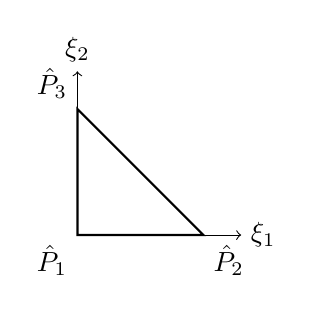
\begin{tikzpicture}[scale=1.6]
  \draw[thick] (0,0) node[anchor=north east]{$\hat P_1$} -- (1,0) node[anchor=north west]{$\hat P_2$} -- (0,1) node[anchor=south east]{$\hat P_3$} -- cycle;
  \draw[->] (0,0) -- (1.3,0) node[anchor=west]{$\xi_1$};
  \draw[->] (0,0) -- (0,1.3) node[anchor=south]{$\xi_2$};
\end{tikzpicture}
\end{center}
It consists of the points with $\xi_1 \geq 0$, $\xi_2 \geq 0$ and $\xi_1 + \xi_2 \leq 1$, and its area is $\frac12$. Its three linear \emph{shape functions}, each equal to $1$ at one vertex and $0$ at the other two, are
\begin{equation}
\label{eqn:shape}
\hat\phi_1(\xi) = 1 - \xi_1 - \xi_2, \qquad \hat\phi_2(\xi) = \xi_1, \qquad \hat\phi_3(\xi) = \xi_2,
\end{equation}
as the nine values at the three vertices below show: $\hat \phi_a(\hat P_b) = \delta_{ab}$ (which is $1$ if $a = b$ and $0$ otherwise). The nine values are
\begin{align*}
\hat\phi_1(0,0) &= 1 - 0 - 0 = 1, & \hat\phi_1(1,0) &= 1 - 1 = 0, & \hat\phi_1(0,1) &= 1 - 1 = 0, \\
\hat\phi_2(0,0) &= 0, & \hat\phi_2(1,0) &= 1, & \hat\phi_2(0,1) &= 0, \\
\hat\phi_3(0,0) &= 0, & \hat\phi_3(1,0) &= 0, & \hat\phi_3(0,1) &= 1 .
\end{align*}
They add up to $1$, as hat functions must: $(1 - \xi_1 - \xi_2) + \xi_1 + \xi_2 = 1$. Their gradients are the vectors of their two partial derivatives~(\ref{eqn:t1_gradient})~[\,$\nabla f = (\partial f/\partial x_1, \partial f/\partial x_2)$\,]. For $\hat\phi_1$, $\partial(1 - \xi_1 - \xi_2)/\partial\xi_1 = -1$ and $\partial(1 - \xi_1 - \xi_2)/\partial\xi_2 = -1$; for $\hat\phi_2 = \xi_1$ the two partial derivatives are $1$ and $0$; for $\hat\phi_3 = \xi_2$ they are $0$ and $1$. So the gradients are constant:
\begin{equation}
\label{eqn:shape_gradients}
\hat \nabla \hat\phi_1 = (-1, -1), \qquad \hat \nabla \hat\phi_2 = (1, 0), \qquad \hat \nabla \hat\phi_3 = (0, 1).
\end{equation}
The hat on $\hat\nabla$ is a reminder that these are derivatives with respect to the reference coordinates $\xi$.

\subsection{The map to a face in space}

The affine map that takes the reference triangle onto a face $f$ with vertices $x_1, x_2, x_3$ (local numbering, in the order of the face) is
\begin{equation}
\label{eqn:affine}
F(\xi) = x_1 + B\, \xi, \qquad B = \big[\, x_2 - x_1 \;\; x_3 - x_1 \,\big] \in \R^{3 \times 2}.
\end{equation}
Written out, $F(\xi) = x_1 + \xi_1 e_1 + \xi_2 e_2$, with the edges $e_1 = x_2 - x_1$ and $e_2 = x_3 - x_1$ of the face, the columns of $B$. It takes $\hat P_1, \hat P_2, \hat P_3$ to $x_1, x_2, x_3$: for instance $F(1, 0) = x_1 + e_1 = x_2$. It takes the edges $\hat e_1, \hat e_2$ of the reference triangle to the edges $e_1$ and $e_2$ of the face (Figure~\ref{fig:reference}), and the midpoint $(\frac12, \frac12)$ of the third reference edge to $x_1 + \frac12 e_1 + \frac12 e_2 = \frac12(x_2 + x_3)$, the midpoint of the third edge of the face. So the numbers $\xi_1, \xi_2$ are coordinates on the face, measured along its two edges: every point of the face is $F(\xi)$ for exactly one $\xi$ of $\hat K$.

\begin{figure}[t]
\centering
\begin{minipage}[c]{0.5\textwidth}\centering\adjustbox{max width=\linewidth}{\begin{tikzpicture}[scale=1.8]
  \draw[->, gray] (0,0) -- (1.35,0) node[right] {$\xi_1$};
  \draw[->, gray] (0,0) -- (0,1.35) node[above] {$\xi_2$};
  \filldraw[draw=black, fill=gray!12, thick] (0,0) -- (1,0) -- (0,1) -- cycle;
  \fill (0,0) circle (0.8pt) node[below left] {$\hat P_1$};
  \fill (1,0) circle (0.8pt) node[below] {$\hat P_2$};
  \fill (0,1) circle (0.8pt) node[left] {$\hat P_3$};
  \draw[-{Stealth[length=2mm]}, very thick, blue!70!black] (0,0) -- (1,0) node[midway, below] {$\hat e_1$};
  \draw[-{Stealth[length=2mm]}, very thick, blue!70!black] (0,0) -- (0,1) node[midway, left] {$\hat e_2$};
  \draw[-{Stealth[length=3mm]}, thick] (1.25,0.6) to[bend left=20] node[above] {$F(\xi) = x_1 + B\xi$} (2.4,0.6);
\end{tikzpicture}
}\end{minipage}\hfill
\begin{minipage}[c]{0.45\textwidth}\centering\adjustbox{max width=\linewidth}{% generated by make_figures.py
\begin{tikzpicture}[]
\filldraw[draw=black, fill=orange!15, thick] (5.7405,-2.1940) -- (10.5901,-1.0635) -- (9.3586,1.9468) -- cycle;
\draw[-{Stealth[length=2.2mm]}, very thick, blue!70!black] (5.7405,-2.1940) -- (10.5901,-1.0635) node[below right] {$e_1 = x_2 - x_1$};
\draw[-{Stealth[length=2.2mm]}, very thick, blue!70!black] (5.7405,-2.1940) -- (9.3586,1.9468) node[left] {$e_2 = x_3 - x_1$};
\fill[fill=black] (5.7405,-2.1940) circle (1.2pt) node[below] {$x_1$};
\fill[fill=black] (10.5901,-1.0635) circle (1.2pt) node[right] {$x_2$};
\fill[fill=black] (9.3586,1.9468) circle (1.2pt) node[above] {$x_3$};
\end{tikzpicture}
}\end{minipage}
\caption{The affine map from the reference triangle to a face in space. The columns of $B$ are the images of the reference edges.}
\label{fig:reference}
\end{figure}

\paragraph{The hats are the shape functions in other coordinates.} The function $\phi_a(F(\xi))$, the hat of vertex $a$ evaluated at the point with coordinates $\xi$, is linear in $\xi$ (a linear function composed with an affine map), and it takes the values $1$ at the vertex $a$ and $0$ at the other two, like $\hat\phi_a$. A linear function is determined by its three vertex values, so
\begin{equation*}
\phi_a(F(\xi)) = \hat\phi_a(\xi) \qquad \text{for every } \xi \in \hat K .
\end{equation*}
In the plane we would write $\phi_a = \hat\phi_a \circ F^{-1}$ and differentiate, inverting the $2\times 2$ matrix $B$. Here $B$ is $3 \times 2$: it maps the plane of $\xi$ onto the plane of the face, which is a plane in space, and has no inverse. We do not need one. What we need is the gradient of $\phi_a$, a vector in the plane of the face, and the identity above, differentiated, determines it.

\paragraph{The chain rule for an affine map.} We want the derivative of the left side, $\phi_a(F(\xi))$, with respect to $\xi_m$, $m \in \{1, 2\}$. A partial derivative is a directional derivative along an axis: increase $\xi_m$ by $s$, keep the other coordinate fixed, and differentiate at $s = 0$,
\begin{equation*}
\frac{\partial}{\partial\xi_m}\, \phi_a(F(\xi)) = \frac{d}{ds}\, \phi_a\big(F(\xi + s\,\varepsilon_m)\big)\Big|_{s=0} .
\end{equation*}
First see where the point goes. Substitute $\xi + s\,\varepsilon_m$ into~(\ref{eqn:affine})~[\,$F(\xi) = x_1 + B\xi$\,]:
\begin{align*}
F(\xi + s\, \varepsilon_m) &= x_1 + B\,(\xi + s\,\varepsilon_m) \\
&= x_1 + B\xi + s\, B\varepsilon_m \quad \text{(distribute $B$)}\\
&= F(\xi) + s\, e_m \quad \text{($x_1 + B\xi = F(\xi)$; $B\varepsilon_m$ is column $m$ of $B$)} .
\end{align*}
Because $F$ is affine, the point moves along a straight line through $F(\xi)$ in the direction of the edge $e_m$, exactly. Substituting this into the derivative:
\begin{align*}
\frac{\partial}{\partial\xi_m}\, \phi_a(F(\xi)) &= \frac{d}{ds}\, \phi_a\big(F(\xi) + s\, e_m\big)\Big|_{s=0} \\
&= e_m(\phi_a) \quad \text{(definition~(\ref{eqn:t1_dirderiv}) of the directional derivative)}\\
&= \nabla\phi_a \cdot e_m \quad \text{(property~(\ref{eqn:t1_gradient}) of the gradient)} ,
\end{align*}
where~(\ref{eqn:t1_dirderiv}) is [\,$X(f) = \frac{d}{ds}f(x + sX)|_{s=0}$\,] and~(\ref{eqn:t1_gradient}) is [\,$X(f) = \nabla f\cdot X$\,], here at the point $x = F(\xi)$ and in the direction $X = e_m$. This is the \emph{chain rule} in the case we need: the derivative of a composition is the gradient of the outer function applied to the derivative $\partial F/\partial\xi_m = e_m$ of the inner one.

\paragraph{Two equations for the gradient.} Write $g = \nabla \phi_a$ for the unknown gradient, a vector of $\R^3$ in the plane of the face. Differentiate both sides of the identity $\phi_a(F(\xi)) = \hat\phi_a(\xi)$ with respect to $\xi_1$, and then with respect to $\xi_2$. On the left the chain rule gives $g\cdot e_1$ and $g\cdot e_2$; on the right we get the two entries of $\hat\nabla\hat\phi_a$, which we write $(\hat\nabla\hat\phi_a)_1$ and $(\hat\nabla\hat\phi_a)_2$:
\begin{equation*}
e_1\cdot g = (\hat\nabla\hat\phi_a)_1, \qquad e_2\cdot g = (\hat\nabla\hat\phi_a)_2 .
\end{equation*}
The rows of $B^T$ are $e_1^T$ and $e_2^T$, so $B^T g$ is the column of the two inner products, and the two equations are one matrix equation:
\begin{equation*}
B^T g = \begin{pmatrix} e_1^T g \\ e_2^T g\end{pmatrix} = \begin{pmatrix} e_1 \cdot g \\ e_2\cdot g\end{pmatrix} = \hat\nabla \hat\phi_a .
\end{equation*}
In words: the slope of the hat along each edge of the face equals the slope of the shape function along the corresponding reference edge.

\paragraph{Solving them.} These are two equations for three unknowns, the components of $g$. The missing condition is that $g$ lies in the plane of the face, which is spanned by the columns of $B$. So $g = B c$ for some $c \in \R^2$, the coordinates of $g$ along the two edges. Substitute $g = Bc$, in parentheses, into $B^Tg = \hat\nabla\hat\phi_a$:
\begin{align*}
B^T (B c) &= \hat\nabla \hat\phi_a \\
(B^T B)\, c &= \hat\nabla \hat\phi_a \quad \text{(associativity: a } 2\times 2 \text{ system for } c\text{)} \\
c &= (B^T B)^{-1} \hat\nabla \hat\phi_a \quad \text{(multiply by the inverse on the left)} \\
g &= B c = B (B^T B)^{-1} \hat\nabla \hat\phi_a \quad \text{(back to } \R^3\text{)}.
\end{align*}

\paragraph{The Gram matrix and its inverse.} The entry $(m, m')$ of $B^TB$ is row $m$ of $B^T$ times column $m'$ of $B$, that is $e_m^T e_{m'} = e_m \cdot e_{m'}$. So $B^T B$ is the \emph{Gram matrix} of the two edges:
\begin{equation*}
B^T B = \begin{pmatrix} e_1\cdot e_1 & e_1\cdot e_2 \\ e_1\cdot e_2 & e_2\cdot e_2\end{pmatrix} .
\end{equation*}
A symmetric $2\times 2$ matrix with entries $p, q, q, r$ has the inverse
\begin{equation*}
\begin{pmatrix} p & q \\ q & r\end{pmatrix}^{-1} = \frac{1}{pr - q^2}\begin{pmatrix} r & -q \\ -q & p\end{pmatrix},
\end{equation*}
because the product of the matrix with the matrix on the right is $pr - q^2$ times the identity,
\begin{equation*}
\begin{pmatrix} p & q \\ q & r\end{pmatrix}\begin{pmatrix} r & -q \\ -q & p\end{pmatrix} = \begin{pmatrix} pr - q^2 & -pq + qp \\ qr - rq & -q^2 + rp\end{pmatrix} = \begin{pmatrix} pr - q^2 & 0 \\ 0 & pr - q^2\end{pmatrix}
\end{equation*}
With $p = e_1\cdot e_1 = |e_1|^2$, $q = e_1\cdot e_2$, $r = |e_2|^2$, the determinant is $|e_1|^2|e_2|^2 - (e_1\cdot e_2)^2$. Write $\theta$ for the angle between the two edges, so that $e_1\cdot e_2 = |e_1||e_2|\cos\theta$ and $|e_1\times e_2| = |e_1||e_2|\sin\theta$. Then
\begin{align*}
|e_1|^2|e_2|^2 - (e_1\cdot e_2)^2 &= |e_1|^2|e_2|^2 - |e_1|^2|e_2|^2\cos^2\theta \\
&= |e_1|^2|e_2|^2\,(1 - \cos^2\theta) \quad \text{(factor out)}\\
&= |e_1|^2|e_2|^2\sin^2\theta = |e_1\times e_2|^2 \quad (\sin^2 + \cos^2 = 1) \\
&= (2A_f)^2 = 4A_f^2 \quad \text{(by~(\ref{eqn:face_normal}), } A_f = \tfrac12|e_1\times e_2|\text{)} .
\end{align*}
This is Lagrange's identity. The determinant is positive for any triangle of positive area, so the inverse exists:
\begin{equation*}
(B^TB)^{-1} = \frac{1}{4A_f^2}\begin{pmatrix} e_2\cdot e_2 & -e_1\cdot e_2 \\ -e_1\cdot e_2 & e_1\cdot e_1\end{pmatrix} .
\end{equation*}

\paragraph{The three gradients written out.} Now substitute this inverse and the three reference gradients~(\ref{eqn:shape_gradients})~[\,$\hat\nabla\hat\phi_1 = (-1,-1),\ \hat\nabla\hat\phi_2 = (1,0),\ \hat\nabla\hat\phi_3 = (0,1)$\,] into $c = (B^TB)^{-1}\hat\nabla\hat\phi_a$ and $g = Bc = c_1 e_1 + c_2 e_2$. For $a = 2$ the inverse applied to $(1, 0)$ is its first column, and for $a = 3$, applied to $(0, 1)$, its second column:
\begin{align*}
c^{(2)} &= \frac{1}{4A_f^2}\begin{pmatrix} e_2\cdot e_2 \\ -e_1\cdot e_2\end{pmatrix}, & \nabla\phi_2 &= \frac{(e_2\cdot e_2)\, e_1 - (e_1\cdot e_2)\, e_2}{4A_f^2} , \\
c^{(3)} &= \frac{1}{4A_f^2}\begin{pmatrix} -e_1\cdot e_2 \\ e_1\cdot e_1\end{pmatrix}, & \nabla\phi_3 &= \frac{(e_1\cdot e_1)\, e_2 - (e_1\cdot e_2)\, e_1}{4A_f^2} .
\end{align*}
For $a = 1$, $(-1, -1) = -(1, 0) - (0, 1)$, and the map $\hat\nabla\hat\phi_a \mapsto g$ is linear, so $\nabla\phi_1 = -\nabla\phi_2 - \nabla\phi_3$. To check $\nabla\phi_2$ against its two equations, take its inner products with the edges:
\begin{align*}
\nabla\phi_2\cdot e_1 &= \frac{(e_2\cdot e_2)(e_1\cdot e_1) - (e_1\cdot e_2)(e_2\cdot e_1)}{4A_f^2} = \frac{4A_f^2}{4A_f^2} = 1 , \\
\nabla\phi_2\cdot e_2 &= \frac{(e_2\cdot e_2)(e_1\cdot e_2) - (e_1\cdot e_2)(e_2\cdot e_2)}{4A_f^2} = 0 ,
\end{align*}
which are $(\hat\nabla\hat\phi_2)_1 = 1$ and $(\hat\nabla\hat\phi_2)_2 = 0$, as required. The answer is a fixed $3\times 2$ matrix per face, $B(B^TB)^{-1}$, applied to the three constant reference gradients.
\begin{prop}
\label{prop:gradient}
On the face, $\nabla \phi_a = B (B^T B)^{-1}\, \hat\nabla \hat\phi_a$, and this vector lies in the plane of the face.
\end{prop}
The matrix $B (B^T B)^{-1}$ is the transpose of the Moore--Penrose pseudo-inverse $B^+ = (B^T B)^{-1} B^T$ of $B$ (transpose it with $(XY)^T = Y^T X^T$ and use that $B^T B$ is symmetric). For a triangle in the plane, where $B$ is a square invertible $2\times 2$ matrix, $(B^T B)^{-1} = B^{-1} B^{-T}$ and so $B (B^T B)^{-1} = B B^{-1} B^{-T} = B^{-T}$, the familiar formula of the planar finite element method. The formula for a triangle in space is the planar formula with the inverse replaced by the pseudo-inverse.

\paragraph{The code.} The gradients are computed at the start of \code{AssembleStiffness\-Element\-Embedded2}, which receives the three vertices of the face in the array \code{v}, in the order of the face (zero-based, \code{v[0]} is $x_1$):
\lstinputlisting[firstline=347, lastline=368, firstnumber=347]{../src/FEM.cpp}
Lines~354--356 fill $B$ row by row: row $0$ holds the $x$ components of the two edges, row $1$ the $y$ components, row $2$ the $z$ components, so that column $0$ is $e_1 = x_2 - x_1$ and column $1$ is $e_2 = x_3 - x_1$, as in~(\ref{eqn:affine})~[\,$B = [\,x_2 - x_1\;\;x_3 - x_1\,]$\,]. Line~358 computes \code{Binv} $= ((B^T B)^{-1} B^T)^T = B (B^T B)^{-1}$, the matrix of Proposition~\ref{prop:gradient}; the name and the comments of lines~362--364, which write $B^{-T}$, come from the planar method, of which this is the extension. Line~360 is the area $A_f = \frac12 |e_1 \times e_2|$, recomputed here rather than read from \code{face\_areas}. Lines~366--368 apply $C = $ \code{Binv} to the three reference gradients~(\ref{eqn:shape_gradients})~[\,$\hat\nabla\hat\phi_1 = (-1,-1),\ \hat\nabla\hat\phi_2 = (1,0),\ \hat\nabla\hat\phi_3 = (0,1)$\,]. Applying a matrix to $(1, 0)$ or $(0, 1)$ picks its first or second column, and applying it to $(-1, -1)$ gives minus the sum of its columns:
\begin{equation}
\label{eqn:gradN}
\nabla \phi_1 = -C_{:,1} - C_{:,2}, \qquad \nabla \phi_2 = C_{:,1}, \qquad \nabla \phi_3 = C_{:,2}, \qquad C = \code{Binv},
\end{equation}
which is \code{gradN[0]}, \code{gradN[1]}, \code{gradN[2]}, written component by component. (The function \code{Gradient}, lines~239--264, computes the same three vectors as the columns of a $3\times 3$ matrix; it is not used by the solver.) The three gradients add up to zero, as they must, since the three hat functions add up to $1$ and the gradient of a constant is zero.

\paragraph{The gradients as a reciprocal frame.} The equations $B^T g = \hat\nabla\hat\phi_a$ have a simple reading for $a = 2, 3$. With $\hat\nabla\hat\phi_2 = (1, 0)$ and $\hat\nabla\hat\phi_3 = (0, 1)$ they say
\begin{equation*}
\nabla\phi_2\cdot e_1 = 1, \qquad \nabla\phi_2\cdot e_2 = 0, \qquad \nabla\phi_3\cdot e_1 = 0, \qquad \nabla\phi_3\cdot e_2 = 1 .
\end{equation*}
So $\nabla\phi_2$ and $\nabla\phi_3$ are the two vectors of the plane of the face that are dual to the edges: each has inner product $1$ with one edge and $0$ with the other. Such a pair is called the \emph{reciprocal frame} of $(e_1, e_2)$, written $e^1, e^2$ (Figure~\ref{fig:gradient}); $e^1$ is orthogonal to $e_2$ and $e^2$ is orthogonal to $e_1$. The reciprocal frame reads off the edge coordinates of a point: a point of the face is $y = x_1 + \xi_1 e_1 + \xi_2 e_2$, and $e^1\cdot(y - x_1) = \xi_1$, $e^2 \cdot (y - x_1) = \xi_2$. Since $\phi_2 = \xi_1$ and $\phi_3 = \xi_2$ on the face, $\phi_2(y) = e^1\cdot(y - x_1)$ and $\phi_3(y) = e^2\cdot(y - x_1)$, linear functions with the gradients $e^1$ and $e^2$, which is the same result seen from another side. Part~\ref{part:ga} builds the gradients in this way.

\paragraph{Face coordinates.} The element matrix will combine the gradients with the transported vectors $R_i^f u_i$, which are stored by their coordinates in the face frame. So the gradients are expressed in the same coordinates:
\begin{equation}
\label{eqn:grad_face}
g_a^f = T_f^T\, \nabla \phi_a \in \R^2 .
\end{equation}
In the code this is line~371, \code{Tf = face\_tangent\_space[face.ID]}, and then \code{grad\_i = Tf.transpose() * gradN[i]} (lines~377--378, shown in Section~\ref{section:element}). Changing to face coordinates does not change inner products of gradients:
\begin{equation*}
g_a^f \cdot g_b^f = (T_f^T \nabla\phi_a)^T (T_f^T\nabla\phi_b) = \nabla\phi_a^T\, (T_f T_f^T)\, \nabla\phi_b = \nabla\phi_a \cdot \nabla \phi_b ,
\end{equation*}
because $T_f T_f^T$ is the projection onto the plane of the face, (\ref{eqn:frame})~[\,$T = [\,t\;\;b\,],\ T^TT = I_2,\ TT^T = I_3 - nn^T$\,], and $\nabla\phi_b$ already lies in that plane. So the projection does not change the stiffness; it only expresses the gradients in the same coordinates as the transported vectors.
\begin{figure}[t]
\centering
\adjustbox{max width=\linewidth}{% the gradient of a hat function, and the reciprocal frame
\begin{tikzpicture}[scale=2.2]
  \coordinate (x1) at (0,0); \coordinate (x2) at (2,0.2); \coordinate (x3) at (0.6,1.3);
  \filldraw[draw=black, fill=orange!12] (x1) -- (x2) -- (x3) -- cycle;
  \draw[-{Stealth[length=2mm]}, very thick, blue!70!black] (x1) -- (x2) node[midway, below] {$e_1$};
  \draw[-{Stealth[length=2mm]}, very thick, blue!70!black] (x1) -- (x3) node[midway, left] {$e_2$};
  % reciprocal frame: e^1 is orthogonal to e_2, e^2 orthogonal to e_1 (computed: B (B^T B)^{-1})
  \pgfmathsetmacro{\aa}{2*2+0.2*0.2} \pgfmathsetmacro{\ab}{2*0.6+0.2*1.3} \pgfmathsetmacro{\bb}{0.6*0.6+1.3*1.3}
  \pgfmathsetmacro{\det}{\aa*\bb-\ab*\ab}
  \pgfmathsetmacro{\rax}{( \bb*2-\ab*0.6)/\det} \pgfmathsetmacro{\ray}{( \bb*0.2-\ab*1.3)/\det}
  \pgfmathsetmacro{\rbx}{(-\ab*2+\aa*0.6)/\det} \pgfmathsetmacro{\rby}{(-\ab*0.2+\aa*1.3)/\det}
  \coordinate (c) at (0.87,0.5);
  \draw[-{Stealth[length=2mm]}, very thick, red!70!black] (c) -- ++(\rax,\ray) node[right] {$e^1 = \nabla\phi_2$};
  \draw[-{Stealth[length=2mm]}, very thick, red!70!black] (c) -- ++(\rbx,\rby) node[left] {$e^2 = \nabla\phi_3$};
  \draw[-{Stealth[length=2mm]}, very thick, red!40!black] (c) -- ++({-\rax-\rbx},{-\ray-\rby}) node[below left] {$\nabla\phi_1$};
  \fill (x1) circle (0.8pt) node[below left] {$x_1$};
  \fill (x2) circle (0.8pt) node[below right] {$x_2$};
  \fill (x3) circle (0.8pt) node[above] {$x_3$};
  % height from x2 to the opposite edge
  \draw[dashed, gray] (x2) -- ($(x1)!(x2)!(x3)$) node[midway, above, sloped, font=\scriptsize] {$h_2 = 1/|\nabla\phi_2|$};
\end{tikzpicture}
}
\caption{The gradients of the hat functions of a face. $\nabla \phi_2$ is orthogonal to the edge opposite to $x_2$, points towards $x_2$, and has length $1/h_2$, the reciprocal of the height; the gradients $\nabla\phi_2 = e^1$ and $\nabla\phi_3 = e^2$ form the \emph{reciprocal frame} of the edges $e_1, e_2$ ($e^k \cdot e_m = \delta_{km}$), and the three gradients add up to zero.}
\label{fig:gradient}
\end{figure}

\begin{example}
\label{ex:triangle}
Take the triangle $x_1 = (0, 0, 0)$, $x_2 = (2, 0, 0)$, $x_3 = (0, 1, 1)$ of Figure~\ref{fig:worked_triangle}. Its edges are $e_1 = x_2 - x_1 = (2, 0, 0)$ and $e_2 = x_3 - x_1 = (0, 1, 1)$. The entries of the Gram matrix are
\begin{equation*}
e_1\cdot e_1 = 4, \qquad e_1\cdot e_2 = 2\cdot 0 + 0\cdot 1 + 0\cdot 1 = 0, \qquad e_2\cdot e_2 = 0 + 1 + 1 = 2 ,
\end{equation*}
and its determinant is $4\cdot 2 - 0^2 = 8$. The cross product is $e_1\times e_2 = (0\cdot 1 - 0\cdot 1,\; 0\cdot 0 - 2\cdot 1,\; 2\cdot 1 - 0\cdot 0) = (0, -2, 2)$, of length $\sqrt 8$, so $A_f = \frac12\sqrt 8 = \sqrt 2$ and $4A_f^2 = 8$, the determinant, as Lagrange's identity says. So
\begin{equation*}
B = \begin{pmatrix} 2 & 0 \\ 0 & 1 \\ 0 & 1 \end{pmatrix}, \quad B^T B = \begin{pmatrix} 4 & 0 \\ 0 & 2 \end{pmatrix}, \quad (B^TB)^{-1} = \frac18\begin{pmatrix} 2 & 0 \\ 0 & 4\end{pmatrix} = \begin{pmatrix} 1/4 & 0 \\ 0 & 1/2\end{pmatrix},
\end{equation*}
and
\begin{equation*}
B (B^T B)^{-1} = \begin{pmatrix} 2\cdot\frac14 & 0 \\ 0 & 1\cdot\frac12 \\ 0 & 1\cdot\frac12 \end{pmatrix} = \begin{pmatrix} 1/2 & 0 \\ 0 & 1/2 \\ 0 & 1/2 \end{pmatrix}.
\end{equation*}
The same comes from the formulas for $\nabla\phi_2$ and $\nabla\phi_3$ written out above, with $e_1\cdot e_2 = 0$: $\nabla\phi_2 = \frac{2\, e_1 - 0\, e_2}{8} = \frac{e_1}{4} = (\frac12, 0, 0)$ and $\nabla\phi_3 = \frac{4\, e_2 - 0\, e_1}{8} = \frac{e_2}{2} = (0, \frac12, \frac12)$. The edges are orthogonal, so the reciprocal frame is just $e_k / |e_k|^2$. By~(\ref{eqn:gradN})~[\,$\nabla\phi_1 = -C_{:,1} - C_{:,2},\ \nabla\phi_2 = C_{:,1},\ \nabla\phi_3 = C_{:,2}$\,],
\begin{equation*}
\nabla\phi_1 = \left(-\tfrac12, -\tfrac12, -\tfrac12\right), \qquad \nabla\phi_2 = \left(\tfrac12, 0, 0\right), \qquad \nabla\phi_3 = \left(0, \tfrac12, \tfrac12\right),
\end{equation*}
which add up to zero. Check $\nabla\phi_2$: along $e_1$, $\phi_2$ goes from $0$ to $1$, and $\nabla\phi_2 \cdot e_1 = \frac12\cdot 2 = 1$; along $e_2$ it stays $0$, and $\nabla\phi_2 \cdot e_2 = 0$. The normal is $n_f = (0, -2, 2)/\sqrt 8 = (0, -1, 1)/\sqrt2$. The face frame of \code{computeFaceTangentSpace} is $t_f = e_1/|e_1| = (1, 0, 0)$ and
\begin{equation*}
b_f = n_f\times t_f = \tfrac{1}{\sqrt2}\big((-1)\cdot 0 - 1\cdot 0,\; 1\cdot 1 - 0\cdot 0,\; 0\cdot 0 - (-1)\cdot 1\big) = \tfrac{1}{\sqrt 2}(0, 1, 1) .
\end{equation*}
The face coordinates~(\ref{eqn:grad_face})~[\,$g_a^f = T_f^T\nabla\phi_a$\,] are the two inner products $(t_f\cdot\nabla\phi_a,\; b_f\cdot\nabla\phi_a)$; for instance $b_f\cdot\nabla\phi_1 = \frac{1}{\sqrt 2}(0 - \frac12 - \frac12) = -\frac{1}{\sqrt 2}$. The three are
\begin{equation*}
g_1^f = \left(-\tfrac12, -\tfrac{1}{\sqrt2}\right), \qquad g_2^f = \left(\tfrac12, 0\right), \qquad g_3^f = \left(0, \tfrac{1}{\sqrt2}\right),
\end{equation*}
with $1/\sqrt 2 \approx 0.7071$. The inner products of the gradients are the same in either form:
\begin{align*}
\nabla\phi_1\cdot\nabla\phi_1 &= \tfrac14 + \tfrac14 + \tfrac14 = \tfrac34, & |g_1^f|^2 &= \tfrac14 + \tfrac12 = \tfrac34, \\
\nabla\phi_1\cdot\nabla\phi_2 &= -\tfrac14 + 0 + 0 = -\tfrac14, & g_1^f\cdot g_2^f &= -\tfrac14 + 0 = -\tfrac14, \\
\nabla\phi_1\cdot\nabla\phi_3 &= 0 - \tfrac14 - \tfrac14 = -\tfrac12, & g_1^f\cdot g_3^f &= 0 - \tfrac12 = -\tfrac12, \\
\nabla\phi_2\cdot\nabla\phi_2 &= \tfrac14, \quad \nabla\phi_3\cdot\nabla\phi_3 = \tfrac12, & \nabla\phi_2\cdot\nabla\phi_3 &= 0 .
\end{align*}
Multiplying by $A_f = \sqrt 2$, the scalar stiffness $A_f\, \nabla\phi_a \cdot \nabla\phi_b$ of the face is
\begin{equation*}
\sqrt 2 \begin{pmatrix} 3/4 & -1/4 & -1/2 \\ -1/4 & 1/4 & 0 \\ -1/2 & 0 & 1/2 \end{pmatrix} = \begin{pmatrix} 1.0607 & -0.3536 & -0.7071 \\ -0.3536 & 0.3536 & 0 \\ -0.7071 & 0 & 0.7071 \end{pmatrix},
\end{equation*}
whose rows add up to zero, since constants have zero gradient: $\frac34 - \frac14 - \frac12 = 0$, $-\frac14 + \frac14 + 0 = 0$, $-\frac12 + 0 + \frac12 = 0$. The entry $(2, 3)$ vanishes because the angle at $x_1$ is a right angle ($e_1\cdot e_2 = 0$), in agreement with the cotangent formula of the next subsection. The entry $(1, 2)$ is $-\frac12 \cot\theta_3$, with the angle $\theta_3$ at $x_3$, between $x_1 - x_3 = (0, -1, -1)$ and $x_2 - x_3 = (2, -1, -1)$:
\begin{equation*}
\cos\theta_3 = \frac{(x_1 - x_3) \cdot (x_2 - x_3)}{|x_1 - x_3|\, |x_2 - x_3|} = \frac{0 + 1 + 1}{\sqrt 2\, \sqrt 6} = \frac{1}{\sqrt 3},
\end{equation*}
$\sin\theta_3 = \sqrt{1 - \frac13} = \frac{\sqrt 2}{\sqrt 3}$, so $\cot\theta_3 = \cos\theta_3/\sin\theta_3 = \frac{1}{\sqrt 2}$ and $-\frac12 \cot\theta_3 = -\frac{1}{2\sqrt 2} = -\frac{\sqrt 2}{4} = -0.3536$, which is $\sqrt2\cdot(-\frac14)$.
\end{example}

\begin{figure}[t]
\centering
\adjustbox{max width=\linewidth}{% generated by make_figures.py
\begin{tikzpicture}[]
\draw[gray, ->] (0.0000,0.0000) -- (5.0007,-1.7734);
\draw[gray, ->] (0.0000,0.0000) -- (2.6226,1.3209);
\draw[gray, ->] (0.0000,0.0000) -- (0.0000,3.4512);
\filldraw[draw=black, fill=orange!15, thick] (0.0000,0.0000) -- (4.1673,-1.4778) -- (1.7484,3.3457) -- cycle;
\fill[fill=black] (0.0000,0.0000) circle (1.2pt) node[below left] {$x_1$};
\fill[fill=black] (4.1673,-1.4778) circle (1.2pt) node[below] {$x_2$};
\fill[fill=black] (1.7484,3.3457) circle (1.2pt) node[above] {$x_3$};
\draw[-{Stealth[length=2.2mm]}, very thick, red!70!black] (1.9719,0.6226) -- (0.0559,-0.6808) node[below] {$\nabla\phi_1$};
\draw[-{Stealth[length=2.2mm]}, very thick, red!70!black] (1.9719,0.6226) -- (3.0137,0.2532) node[right] {$\nabla\phi_2$};
\draw[-{Stealth[length=2.2mm]}, very thick, red!70!black] (1.9719,0.6226) -- (2.8461,2.2955) node[above] {$\nabla\phi_3$};
\draw[-{Stealth[length=2.2mm]}, thick, blue!70!black] (1.9719,0.6226) -- (1.1065,1.4070) node[left] {$n_f$};
\node[gray] at (5.2091,-1.8472) {$x$};
\node[gray] at (2.7974,1.4089) {$y$};
\node[gray] at (0.0000,3.6977) {$z$};
\end{tikzpicture}
}
\caption{The triangle of Example~\ref{ex:triangle}, its normal $n_f = (0, -1, 1)/\sqrt 2$, and the gradients of its three hat functions, drawn from the centroid. All three lie in the plane of the face.}
\label{fig:worked_triangle}
\end{figure}

\subsection{A check: the cotangent formula}

The scalar factor of~(\ref{eqn:element_stiffness})~[\,$\mathrm L^f_{ij} = A_f\,(g_i^f\cdot g_j^f)\,(R_i^f)^TR_j^f$\,] has a classical closed form, which connects the finite element computation with the cotangent Laplacian of geometry processing (\code{CalcCotangentWeights} in \code{Laplacian.cpp}). It also shows that the scalar factor is intrinsic: it depends only on the angles of the triangle. We derive it from the geometric meaning of the gradient (Section~\ref{section:transport}): it is orthogonal to the level lines, and its length is the slope in the steepest direction. Name the three vertices of the face $a$, $b$, $c$, the angle of the triangle at each vertex $\theta_a, \theta_b, \theta_c$, and the length of the edge opposite to each vertex $\ell_a, \ell_b, \ell_c$.

\emph{Step 1: the direction of $\nabla\phi_a$.} Along the edge opposite to $a$, $\phi_a$ is constant (zero at both ends, and linear). So for a direction $X$ along that edge, $X(\phi_a) = 0$, and by~(\ref{eqn:t1_gradient})~[\,$X(f) = \nabla f\cdot X$\,], $\nabla\phi_a\cdot X = 0$: the gradient is orthogonal to the opposite edge. It lies in the plane of the face (Proposition~\ref{prop:gradient}), so it is a multiple of the unit normal $m_a$ of the opposite edge in the plane of the face, which we choose pointing into the triangle:
\begin{equation*}
\nabla\phi_a = \lambda\, m_a \qquad \text{for some number } \lambda .
\end{equation*}

\emph{Step 2: the length of $\nabla\phi_a$.} Walk from the opposite edge to $a$ along $m_a$. The distance is the height $h_a$ of the triangle from $a$, and $\phi_a$ grows linearly from $0$ to $1$ on the way, so its rate of growth along $m_a$ is $1/h_a$. That rate is the directional derivative along the unit vector $m_a$:
\begin{align*}
\frac{1}{h_a} &= m_a(\phi_a) = \nabla\phi_a\cdot m_a \quad \text{(by~(\ref{eqn:t1_gradient}))}\\
&= (\lambda\, m_a)\cdot m_a = \lambda\, |m_a|^2 = \lambda \quad \text{(Step 1, and } |m_a| = 1\text{)} .
\end{align*}
The area is half the base times the height, $A_f = \frac12 \ell_a h_a$, so $\frac{1}{h_a} = \frac{\ell_a}{2A_f}$. Substituting $\lambda = \frac{\ell_a}{2A_f}$ into Step 1:
\begin{equation*}
\nabla \phi_a = \frac{\ell_a}{2 A_f}\, m_a , \qquad \text{and likewise} \qquad \nabla \phi_b = \frac{\ell_b}{2 A_f}\, m_b .
\end{equation*}

\emph{Step 3: the angle between $m_a$ and $m_b$.} The edge opposite to $a$ is $cb$ and the edge opposite to $b$ is $ca$; they meet at $c$, with the angle $\theta_c$. Measure angles in the plane of the face from the direction of $c \to b$, and orient the plane so that $c \to a$ is at the angle $\theta_c$. The inward normal $m_a$ of the edge $cb$ is the direction $c\to b$ turned by $90^\circ$ towards $a$, so it is at the angle $90^\circ$. The inward normal $m_b$ of the edge $ca$ is the direction $c\to a$ turned by $90^\circ$ towards $b$, that is, backwards, so it is at the angle $\theta_c - 90^\circ$. The angle between them is
\begin{equation*}
90^\circ - (\theta_c - 90^\circ) = 180^\circ - \theta_c, \qquad \text{so} \qquad m_a\cdot m_b = \cos(\pi - \theta_c) = -\cos\theta_c .
\end{equation*}

\emph{Step 4: two different vertices.} Substitute Step 2, in parentheses, into the inner product, and then Step 3:
\begin{align*}
A_f\, \nabla \phi_a \cdot \nabla \phi_b &= A_f\, \Big(\frac{\ell_a}{2A_f}\, m_a\Big)\cdot\Big(\frac{\ell_b}{2A_f}\, m_b\Big) \\
&= A_f\, \frac{\ell_a \ell_b}{4 A_f^2}\, m_a\cdot m_b \quad \text{(numbers out of the inner product)}\\
&= \frac{\ell_a \ell_b}{4 A_f}\,(-\cos\theta_c) \quad \text{(cancel one } A_f\text{; Step 3)} .
\end{align*}
The two edges at $c$ have the lengths $\ell_a$ and $\ell_b$, and the area of a triangle is half the product of two sides times the sine of the angle between them: $A_f = \frac12 \ell_a \ell_b \sin\theta_c$, that is $\ell_a\ell_b = 2A_f/\sin\theta_c$. Substituting it, in parentheses:
\begin{align*}
A_f\, \nabla \phi_a \cdot \nabla \phi_b &= -\Big(\frac{2 A_f}{\sin\theta_c}\Big)\,\frac{\cos\theta_c}{4 A_f} \\
&= -\frac{2}{4}\,\frac{\cos\theta_c}{\sin\theta_c} \quad \text{(cancel } A_f\text{)}\\
&= -\frac12 \cot \theta_c .
\end{align*}

\emph{Step 5: the diagonal.} The three hat functions add up to $1$ on the face, so their gradients add up to zero, $\nabla \phi_a = -\nabla \phi_b - \nabla \phi_c$. Substitute it, in parentheses, into one factor of $|\nabla\phi_a|^2 = \nabla\phi_a\cdot\nabla\phi_a$:
\begin{align*}
A_f\, |\nabla\phi_a|^2 &= A_f\, \nabla\phi_a \cdot (-\nabla\phi_b - \nabla\phi_c) \\
&= -A_f\, \nabla\phi_a\cdot\nabla\phi_b - A_f\, \nabla\phi_a\cdot\nabla\phi_c \quad \text{(distribute)}\\
&= -\big(-\tfrac12\cot\theta_c\big) - \big(-\tfrac12\cot\theta_b\big) \quad \text{(Step 4 twice)}\\
&= \tfrac12\cot\theta_b + \tfrac12\cot\theta_c ,
\end{align*}
where Step 4 is used for the pair $a, b$, whose third vertex is $c$, and for the pair $a, c$, whose third vertex is $b$.
\begin{prop}
\label{prop:cotangent}
For two distinct vertices $a, b$ of a face with area $A_f$, $A_f\, \nabla \phi_a \cdot \nabla \phi_b = -\frac12 \cot \theta_c$, where $\theta_c$ is the angle at the third vertex $c$; and $A_f\, |\nabla \phi_a|^2 = \frac12 (\cot \theta_b + \cot \theta_c)$.
\end{prop}
In Example~\ref{ex:triangle}, the entry $(2, 3)$ is $-\frac12\cot\theta_1 = -\frac12\cot 90^\circ = 0$. The entry $(1, 3)$ is $-\frac12\cot\theta_2$, with the angle at $x_2$ between $x_1 - x_2 = (-2, 0, 0)$ and $x_3 - x_2 = (-2, 1, 1)$: $\cos\theta_2 = \frac{4}{2\sqrt 6} = \frac{2}{\sqrt 6}$, $\sin\theta_2 = \sqrt{1 - \frac46} = \frac{1}{\sqrt 3}$, $\cot\theta_2 = \frac{2}{\sqrt 6}\cdot\sqrt 3 = \sqrt 2$, and $-\frac12\cot\theta_2 = -0.7071$, which is $\sqrt 2\cdot(-\frac12)$, as in the matrix. The diagonal entry $(1, 1)$ is $\frac12(\cot\theta_2 + \cot\theta_3) = \frac12(\sqrt 2 + \frac{1}{\sqrt 2}) = \frac{3}{2\sqrt 2} = 1.0607$, which is $\sqrt 2\cdot\frac34$.

\paragraph{Summing over the faces of an edge.} An interior edge $ij$ belongs to two faces. In each of them the coupling of $i$ and $j$ is $-\frac12\cot$ of the angle at the third vertex, the angle opposite to the edge. Call these two angles $\alpha_{ij}$ and $\beta_{ij}$ (Figure~\ref{fig:cotangent}). Adding the two contributions, the off-diagonal scalar stiffness of the edge is $-\frac12 (\cot \alpha_{ij} + \cot \beta_{ij})$, the \emph{cotangent weight} of the edge.
\begin{figure}[t]
\centering
\adjustbox{max width=\linewidth}{% the cotangent weight of an edge: the angles opposite to it in its two faces
\begin{tikzpicture}[scale=2]
  \coordinate (i) at (0,0); \coordinate (j) at (2,0); \coordinate (k) at (1.2,1.1); \coordinate (l) at (0.7,-0.9);
  \filldraw[draw=black, fill=orange!12] (i) -- (j) -- (k) -- cycle;
  \filldraw[draw=black, fill=blue!10] (i) -- (l) -- (j) -- cycle;
  \draw[very thick] (i) -- (j);
  \pic[draw, angle radius=0.35cm, "$\alpha_{ij}$", angle eccentricity=1.7] {angle = i--k--j};
  \pic[draw, angle radius=0.35cm, "$\beta_{ij}$", angle eccentricity=1.7] {angle = j--l--i};
  \fill (i) circle (0.8pt) node[left] {$x_i$};
  \fill (j) circle (0.8pt) node[right] {$x_j$};
  \node[font=\footnotesize, align=center] at (1,-1.35) {$\mathrm L_{ij} = -\frac12 (\cot\alpha_{ij} + \cot\beta_{ij})\, (R_i^f)^T R_j^f$ \\ (scalar part summed over the two faces)};
\end{tikzpicture}
}
\caption{The two angles opposite to an edge $ij$ in its two faces. The scalar part of the stiffness block of the edge is the cotangent weight; the connection Laplacian multiplies it by the transport from $j$ to $i$.}
\label{fig:cotangent}
\end{figure}
The connection Laplacian~(\ref{eqn:element_stiffness}) is therefore the cotangent Laplacian with a $2 \times 2$ transport on every edge, as in the discrete connection Laplacians of geometry processing \cite{Knoppel2013, Sharp2019}; the finite element derivation explains where both factors come from.

%%% ----------------------------------------------------------------------
\section{Stage 7, Completed: The Element Matrices}
\label{section:element}

\paragraph{What we want.} The global matrices~(\ref{eqn:global_blocks}) are integrals over the whole surface, and every integral over the surface is a sum of integrals over the faces. On one face only three hat functions are nonzero, those of its three vertices, so a face contributes only to the blocks that couple its vertices with each other. This suggests the organization of every finite element code: compute, face by face, a small \emph{element matrix} that holds the contribution of the face, and then add the element matrices into the global one. This section computes the element matrices; Section~\ref{section:assembly} adds them up.

\subsection{The element stiffness matrix}

On one face, the hat functions of its three vertices are the only nonzero ones, so the face contributes to the $3 \times 3$ blocks of $\mathrm L$ indexed by its vertices, a $6 \times 6$ \emph{element matrix} in the local numbering $a, b \in \{1, 2, 3\}$:
\begin{equation}
\label{eqn:element_matrix}
\mathrm L^f = \begin{pmatrix} \mathrm L^f_{11} & \mathrm L^f_{12} & \mathrm L^f_{13} \\ \mathrm L^f_{21} & \mathrm L^f_{22} & \mathrm L^f_{23} \\ \mathrm L^f_{31} & \mathrm L^f_{32} & \mathrm L^f_{33} \end{pmatrix}, \qquad \mathrm L^f_{ab} = A_f\, (g_a^f \cdot g_b^f)\, (R_a^f)^T R_b^f \in \R^{2 \times 2}.
\end{equation}
Each block is~(\ref{eqn:element_stiffness}) for one pair of vertices of the face. This is \code{AssembleStiffness\-Element\-Embedded2}. Its first part, which computes $B$, \code{Binv}, $A_f$ (\code{faceArea}) and the three gradients, was shown in Section~\ref{section:gradients}; here is the rest, which fills the blocks:
\lstinputlisting[firstline=369, lastline=393, firstnumber=369]{../src/FEM.cpp}
Line~369 sets the $6 \times 6$ matrix to zero and line~371 fetches the face frame $T_f$. The two loops run over the local vertices, \code{i} for the test function (the block row $a$) and \code{j} for the unknown (the block column $b$), both counted from zero. Line~375 skips the pairs with $a < b$, because the matrix is symmetric and those blocks are written together with their transposes. For each remaining pair:
\begin{itemize}
\item lines~377--378 are the face coordinates~(\ref{eqn:grad_face})~[\,$g_a^f = T_f^T\nabla\phi_a$\,] of the two gradients, $g_a^f$ and $g_b^f$;
\item lines~379--380 are the two transports $R_a^f$ and $R_b^f$ of~(\ref{eqn:connection})~[\,$R_i^f = T_f^TQ_{i\to f}T_i$\,], computed by \code{Rvf}. (They are recomputed for every pair, which repeats work but does not change the result.)
\item On the diagonal, $a = b$, line~383 writes $A_f\, |g_a^f|^2\, I_2$. This is~(\ref{eqn:element_matrix}) with the product $(R_a^f)^T R_a^f$ replaced by $I_2$, which it equals exactly, by Proposition~\ref{prop:connection_rotation}; the code takes the shortcut.
\item Off the diagonal, line~387 writes the block $(a, b)$, $A_f\, (g_a^f\cdot g_b^f)\, (R_a^f)^T R_b^f$, and line~388 the block $(b, a)$, $A_f\, (g_b^f\cdot g_a^f)\, (R_b^f)^T R_a^f$, which is its transpose.
\end{itemize}
The block $(a, b)$ starts at row $2a$ and column $2b$ of the element matrix (\code{block<2,2>(i * 2, j * 2)}), because each vertex has two coordinates, in the same zero-based count as the global index $2i + k$ of Section~\ref{section:geometry}.

To picture the $6\times 6$ matrix, consider first a flat mesh in which all frames agree, so that every $R_a^f = I_2$. Then each block is a number times $I_2$: the scalar element matrix of the face, with every entry $s_{ab} = A_f\, g_a^f\cdot g_b^f$ replaced by the block $s_{ab} I_2$, and the two coordinates do not interact. For the triangle of Example~\ref{ex:triangle} with such frames, the first block row would be $(1.0607\, I_2,\; -0.3536\, I_2,\; -0.7071\, I_2)$. On a curved mesh, or with frames that do not agree, the diagonal blocks stay the same and each off-diagonal block becomes its number times the rotation $(R_a^f)^TR_b^f$, which mixes the two coordinates.

\paragraph{Exactness of the integration.} The integrand of~(\ref{eqn:element_stiffness})~[\,$\mathrm L^f_{ij} = A_f\,(g_i^f\cdot g_j^f)\,(R_i^f)^TR_j^f$\,] is constant on the face, so ``area times integrand'' is the exact integral, with no quadrature error. For higher order elements the gradients would vary and a quadrature rule would be needed; with linear elements it is not.

\subsection{The element mass matrix and its lumping}

The mass matrix needs the integrals $\int_f \Psi_{b,l} \cdot \Psi_{a,k}\, dA$ over a face $f$, for two of its vertices $a, b$. Substitute the basis functions~(\ref{eqn:basis})~[\,$\Psi_{a,k}|_f = \phi_a\,T_fR_a^f\varepsilon_k$\,], in parentheses, into the integrand, and simplify one step per line:
\begin{align*}
\Psi_{b,l} \cdot \Psi_{a,k} &= \big(\phi_b\, T_f R_b^f\varepsilon_l\big)\cdot\big(\phi_a\, T_f R_a^f\varepsilon_k\big) \\
&= \phi_a\phi_b\; (T_f R_a^f\varepsilon_k)\cdot (T_f R_b^f \varepsilon_l) \quad \text{(the hats are numbers; reorder)}\\
&= \phi_a\phi_b\; (T_f R_a^f\varepsilon_k)^T (T_f R_b^f \varepsilon_l) \quad (x\cdot y = x^Ty)\\
&= \phi_a\phi_b\; \varepsilon_k^T (R_a^f)^T (T_f^T T_f) R_b^f \varepsilon_l \quad ((XYZ)^T = Z^TY^TX^T)\\
&= \phi_a\phi_b\; \varepsilon_k^T (R_a^f)^T R_b^f \varepsilon_l \quad (T_f^T T_f = I_2)\\
&= \phi_a\phi_b\, \big( (R_a^f)^T R_b^f \big)_{kl} \quad (\varepsilon_k^TX\varepsilon_l = X_{kl}).
\end{align*}
Only the product $\phi_a\phi_b$ varies over the face; the transports are constant, so they come out of the integral:
\begin{equation*}
\int_f \Psi_{b,l} \cdot \Psi_{a,k}\, dA = \Big( \int_f \phi_a \phi_b\, dA \Big)\, \big( (R_a^f)^T R_b^f \big)_{kl} .
\end{equation*}
Everything reduces to the integrals $\int_f \phi_a\phi_b\, dA$ of products of two hats over the face: nine of them, of which six are different, because $\phi_a\phi_b = \phi_b\phi_a$.

\paragraph{From the face to the reference triangle.} These integrals are easiest on the reference triangle, where the hats are the simple shape functions~(\ref{eqn:shape})~[\,$\hat\phi_1 = 1 - \xi_1 - \xi_2,\ \hat\phi_2 = \xi_1,\ \hat\phi_3 = \xi_2$\,]. To move an integral from the face to the reference triangle we need to know how the map~(\ref{eqn:affine})~[\,$F(\xi) = x_1 + B\xi$\,] changes areas. A small rectangle of the reference plane, with corner $\xi$ and sides $d\xi_1$ and $d\xi_2$ along the axes, is mapped, by the computation of the chain rule above [\,$F(\xi + s\varepsilon_m) = F(\xi) + s\,e_m$\,], to the parallelogram with corner $F(\xi)$ and sides $d\xi_1\, e_1$ and $d\xi_2\, e_2$. The area of a parallelogram is the length of the cross product of its sides:
\begin{align*}
|(d\xi_1\, e_1) \times (d\xi_2\, e_2)| &= |e_1 \times e_2|\, d\xi_1\, d\xi_2 \quad \text{(numbers out of the cross product)}\\
&= 2A_f\, d\xi_1\, d\xi_2 \quad \text{(by~(\ref{eqn:face_normal}), } A_f = \tfrac12|e_1\times e_2|\text{)} .
\end{align*}
So every small piece of the reference triangle has its area multiplied by the same constant $2A_f$ (as a check, the reference triangle has area $\frac12$, and $2A_f \cdot \frac12 = A_f$). Cutting both triangles into corresponding small pieces, and using $\phi_a(F(\xi)) = \hat\phi_a(\xi)$ on each piece,
\begin{equation*}
\int_f \phi_a\phi_b\, dA = 2A_f\int_{\hat K}\hat\phi_a\hat\phi_b\, d\xi .
\end{equation*}

\paragraph{The six integrals over the reference triangle.} An integral over $\hat K$ is computed as two nested integrals of one variable: for each $\xi_1$ between $0$ and $1$, the points of the triangle have $\xi_2$ between $0$ and $1 - \xi_1$, so we integrate first in $\xi_2$ over that range and then in $\xi_1$. Write $L = 1 - \xi_1$ for the length of the inner range; it does not depend on $\xi_2$. Two integrals of one variable will be used several times:
\begin{align*}
\int_0^1 (1 - \xi_1)^3\, d\xi_1 &= \Big[-\frac{(1 - \xi_1)^4}{4}\Big]_0^1 = 0 - \Big(-\frac14\Big) = \frac14, \\
\int_0^1 \xi_1(1 - \xi_1)^2\, d\xi_1 &= \int_0^1 (\xi_1 - 2\xi_1^2 + \xi_1^3)\, d\xi_1 \quad \text{(expand the square)}\\
&= \frac12 - \frac23 + \frac14 = \frac{6 - 8 + 3}{12} = \frac{1}{12} .
\end{align*}
\emph{The square of $\hat\phi_2 = \xi_1$.} The integrand does not depend on $\xi_2$, so the inner integral is the integrand times the length $L$:
\begin{align*}
\int_{\hat K} \xi_1^2\, d\xi &= \int_0^1 \Big(\int_0^{1-\xi_1} \xi_1^2\, d\xi_2\Big) d\xi_1 = \int_0^1 \xi_1^2\,(1 - \xi_1)\, d\xi_1 \\
&= \int_0^1 (\xi_1^2 - \xi_1^3)\, d\xi_1 = \frac13 - \frac14 = \frac{1}{12} .
\end{align*}
\emph{The square of $\hat\phi_3 = \xi_2$.} The inner integral is $\int_0^L \xi_2^2\, d\xi_2 = \frac{L^3}{3}$:
\begin{equation*}
\int_{\hat K} \xi_2^2\, d\xi = \int_0^1 \frac{(1 - \xi_1)^3}{3}\, d\xi_1 = \frac13\cdot\frac14 = \frac{1}{12} .
\end{equation*}
\emph{The square of $\hat\phi_1 = 1 - \xi_1 - \xi_2 = L - \xi_2$.} Substitute $t = L - \xi_2$ in the inner integral; $t$ runs from $L$ down to $0$ as $\xi_2$ runs from $0$ to $L$, so the inner integral is $\int_0^L t^2\, dt = \frac{L^3}{3}$, as for $\hat\phi_3$:
\begin{equation*}
\int_{\hat K} (1 - \xi_1 - \xi_2)^2\, d\xi = \int_0^1 \frac{(1 - \xi_1)^3}{3}\, d\xi_1 = \frac{1}{12} .
\end{equation*}
\emph{The product $\hat\phi_2\hat\phi_3 = \xi_1\xi_2$.} The factor $\xi_1$ comes out of the inner integral, which leaves $\int_0^L \xi_2\, d\xi_2 = \frac{L^2}{2}$:
\begin{equation*}
\int_{\hat K} \xi_1\xi_2\, d\xi = \int_0^1 \xi_1\, \frac{(1-\xi_1)^2}{2}\, d\xi_1 = \frac12\cdot\frac{1}{12} = \frac{1}{24} .
\end{equation*}
\emph{The product $\hat\phi_1\hat\phi_2 = \xi_1(L - \xi_2)$.} The factor $\xi_1$ comes out of the inner integral, which leaves $\int_0^L (L - \xi_2)\, d\xi_2 = L^2 - \frac{L^2}{2} = \frac{L^2}{2}$:
\begin{equation*}
\int_{\hat K} \xi_1(1 - \xi_1 - \xi_2)\, d\xi = \int_0^1 \xi_1\, \frac{(1-\xi_1)^2}{2}\, d\xi_1 = \frac{1}{24} .
\end{equation*}
\emph{The product $\hat\phi_1\hat\phi_3 = (L - \xi_2)\,\xi_2$.} The inner integral is $\int_0^L (L\xi_2 - \xi_2^2)\, d\xi_2 = L\,\frac{L^2}{2} - \frac{L^3}{3} = \frac{L^3}{6}$:
\begin{equation*}
\int_{\hat K} (1 - \xi_1 - \xi_2)\,\xi_2\, d\xi = \int_0^1 \frac{(1 - \xi_1)^3}{6}\, d\xi_1 = \frac16\cdot\frac14 = \frac{1}{24} .
\end{equation*}
So the three squares have the integral $\frac{1}{12}$ and the three products of two different shape functions have the integral $\frac{1}{24}$. Multiplying by $2A_f$,
\begin{equation*}
\int_f\phi_a^2\, dA = 2A_f\cdot\frac{1}{12} = \frac{A_f}{6}, \qquad \int_f\phi_a\phi_b\, dA = 2A_f\cdot\frac{1}{24} = \frac{A_f}{12} \quad (a\ne b),
\end{equation*}
that is, $\int_f \phi_a \phi_b\, dA = \frac{A_f}{12} (1 + \delta_{ab})$. As a $3\times 3$ matrix,
\begin{equation*}
\Big[\int_f \phi_a\phi_b\, dA\Big]_{a,b} = \frac{A_f}{12}\begin{pmatrix} 2 & 1 & 1 \\ 1 & 2 & 1 \\ 1 & 1 & 2\end{pmatrix} .
\end{equation*}
So the \emph{consistent} element mass matrix, the exact Galerkin one, has the blocks
\begin{equation}
\label{eqn:consistent_mass}
\mathrm M^f_{ab} = \frac{A_f}{12} (1 + \delta_{ab})\, (R_a^f)^T R_b^f .
\end{equation}

\paragraph{Lumping.} The consistent mass matrix couples each vertex with its neighbors, like the stiffness matrix. The code uses instead the simpler \emph{lumped} mass matrix, which moves all the mass of each row of the scalar factor to the diagonal. The row sum of row $a$ can be computed in two ways. With the numbers just found, one square and two products:
\begin{equation*}
\sum_b \int_f \phi_a \phi_b\, dA = \frac{A_f}{6} + \frac{A_f}{12} + \frac{A_f}{12} = \frac{2A_f + A_f + A_f}{12} = \frac{A_f}{3} .
\end{equation*}
Or with the partition of unity, without computing any product:
\begin{align*}
\sum_b \int_f \phi_a \phi_b\, dA &= \int_f \phi_a \Big(\sum_b \phi_b\Big)\, dA \quad \text{(sum into the integral; factor out } \phi_a\text{)}\\
&= \int_f \phi_a\, dA \quad \Big(\textstyle\sum_b\phi_b = 1\Big)\\
&= 2A_f\int_{\hat K}\xi_1\, d\xi \quad \text{(to the reference triangle, } a = 2\text{)}\\
&= 2A_f\int_0^1 \xi_1(1 - \xi_1)\, d\xi_1 \quad \text{(inner integral: } \xi_1 \text{ times } L\text{)}\\
&= 2A_f\Big(\frac12 - \frac13\Big) = 2A_f\cdot\frac16 = \frac{A_f}{3} ,
\end{align*}
and the same for $a = 1$ and $a = 3$. The lumped matrix keeps these row sums on the diagonal and puts zeros elsewhere:
\begin{equation*}
\frac{A_f}{12}\begin{pmatrix} 2 & 1 & 1 \\ 1 & 2 & 1 \\ 1 & 1 & 2\end{pmatrix} \quad\longrightarrow\quad \frac{A_f}{3}\begin{pmatrix} 1 & 0 & 0 \\ 0 & 1 & 0 \\ 0 & 0 & 1\end{pmatrix} .
\end{equation*}
In blocks, the lumped element mass matrix is
\begin{equation}
\label{eqn:lumped_mass}
\mathrm M^f_{aa} = \frac{A_f}{3}\, I_2, \qquad \mathrm M^f_{ab} = 0 \quad (a \neq b),
\end{equation}
where the transport has disappeared because $(R_a^f)^T R_a^f = I$. For the triangle of Example~\ref{ex:triangle}, with $A_f = \sqrt 2$, the consistent scalar entries are $A_f/6 = 0.2357$ on the diagonal and $A_f/12 = 0.1179$ off it, and the lumped entry is their row sum, $0.2357 + 2\cdot 0.1179 = A_f/3 = 0.4714$.

Lumping keeps two things exactly. The total mass of each row, by construction; and therefore the total mass of the whole matrix, $\sum_a \frac{A_f}{3} = A_f$ per face, so that the masses of all the vertices add up to the area of the surface, as $\int_\Omega 1\, dA$ should. Why is this allowed? The mass matrix multiplies the vector of unknowns, and for a smooth field the values at the three vertices of a small face are nearly equal (after transport), so the row $\sum_b \mathrm M^f_{ab} u_b$ is nearly the row sum times $u_a$: lumping makes an error of the size of the variation of the field across one face, which is of the order of the discretization error that the method makes anyway. It keeps $\mathrm M$ diagonal and positive, and makes $\mathrm M^{-1}$ trivial, which the code uses in Section~\ref{section:solve}. Assembled, the mass of vertex $i$ is one third of the total area of its incident faces, the same for both coordinates: the area of the surface that the vertex ``owns''. This is \code{AssembleDiagonal\-Mass\-Matrix}:
\lstinputlisting[firstline=475, lastline=493, firstnumber=475]{../src/FEM.cpp}
Line~476 creates an empty $2n\times 2n$ sparse matrix. For every face, lines~480--482 take its three vertices, line~483 reads the area $A_f$ computed by \code{computeFaceNormals}, and line~484 is the lumped mass $A_f/3$ of~(\ref{eqn:lumped_mass}). Lines~485--490 add it to the two diagonal entries $2\,\mathrm{ID} + 0$ and $2\,\mathrm{ID} + 1$ of each of the three vertices: the block $\frac{A_f}{3}I_2$, written as its two nonzero entries. This function does the assembly of the next section directly, without forming an element matrix, because the element matrix is diagonal.

\paragraph{What Stage 7 produced.} For every face, the $6\times 6$ element stiffness matrix~(\ref{eqn:element_matrix})~[\,$\mathrm L^f_{ab} = A_f\,(g_a^f\cdot g_b^f)\,(R_a^f)^TR_b^f$\,] and the lumped element mass~(\ref{eqn:lumped_mass})~[\,$\mathrm M^f_{aa} = \tfrac{A_f}{3}I_2$\,], both computed exactly (the stiffness) or with a controlled simplification (the mass), from the reference triangle, the affine map and the chain rule. The geometry of the face enters through $A_f$ and the gradients; the curvature of the surface through the transports. Stage 8 adds them up.

%%% ----------------------------------------------------------------------
\section{Stage 8. Assembly}
\label{section:assembly}

\paragraph{What we want.} The global matrices of Stage 6 from the element matrices of Stage 7, then the source condition, then the solution, read back as vectors. This section does the first step; Section~\ref{section:solve} the rest.

\paragraph{From local to global indices.} The global matrices are sums over the faces, and each face contributes its element matrix at the rows and columns of its own three vertices. To write this as a formula we need a way to pick, out of the global vector $\mathrm u$ of $2n$ numbers, the six numbers that belong to one face. That is a matrix $P_f$ of size $6 \times 2n$, made of zeros and ones: its row $(a, k)$, the row $2(a-1) + k$, has a single $1$, in the column $(f_a, k)$ of coordinate $k$ of the vertex $f_a$:
\begin{equation*}
(P_f)_{(a,k),\,p} = \begin{cases} 1 & \text{if } p = (f_a, k), \\ 0 & \text{otherwise.}\end{cases}
\end{equation*}
Then $(P_f\mathrm u)_{(a,k)} = \sum_p (P_f)_{(a,k),p}\, \mathrm u_p = u_{f_a,k}$: $P_f\mathrm u$ is the local vector of the face, the coordinates of its three vertices in local order. The global matrices are
\begin{equation}
\label{eqn:assembly}
\mathrm L = \sum_f P_f^T\, \mathrm L^f\, P_f, \qquad \mathrm M = \sum_f P_f^T\, \mathrm M^f\, P_f .
\end{equation}

\paragraph{What $P_f^T\mathrm L^f P_f$ is, entry by entry.} Write out the entry $(p, q)$ of the triple product, with the sums over the local rows $(a, k)$ and the local columns $(b, l)$:
\begin{align*}
\big(P_f^T\mathrm L^f P_f\big)_{p,q} &= \sum_{(a,k)}\sum_{(b,l)} (P_f^T)_{p,(a,k)}\, \mathrm L^f_{(a,k),(b,l)}\, (P_f)_{(b,l),q} \\
&= \sum_{(a,k)}\sum_{(b,l)} (P_f)_{(a,k),p}\, \mathrm L^f_{(a,k),(b,l)}\, (P_f)_{(b,l),q} \quad \text{(transpose)} .
\end{align*}
The first factor is $1$ only for the local row with $(f_a, k) = p$, and the last only for the local column with $(f_b, l) = q$; every other term is zero. So
\begin{equation*}
\big(P_f^T\mathrm L^f P_f\big)_{p,q} = \begin{cases} \mathrm L^f_{(a,k),(b,l)} & \text{if } p = (f_a, k) \text{ and } q = (f_b, l), \\ 0 & \text{if } p \text{ or } q \text{ is not a coordinate of a vertex of } f .\end{cases}
\end{equation*}
The product is a $2n\times 2n$ matrix that is zero except at the rows and columns of the three vertices of $f$, where it holds the entries of $\mathrm L^f$, moved to the global positions.

\paragraph{Why the sum is the global matrix.} The reason is the energy. Split the integral over the mesh into the integrals over the faces. On a face only its three vertices have nonzero hats, so the energy of the face is the quadratic form of $\mathrm L^f$ in the local vector $P_f\mathrm u$, by the same computation as for $\mathrm u^T\mathrm L\,\mathrm u$ in Section~\ref{section:r1_element_integrals}. Then, one step per line:
\begin{align*}
\mathrm u^T\mathrm L\,\mathrm u &= \int_{\Omega_h} |\nabla U|^2\, dA = \sum_f \int_f |\nabla U|^2\, dA \quad \text{(sum over the faces)}\\
&= \sum_f (P_f\mathrm u)^T\, \mathrm L^f\, (P_f\mathrm u) \quad \text{(the energy of each face)}\\
&= \sum_f \mathrm u^T\, P_f^T\mathrm L^f P_f\, \mathrm u \quad ((XY)^T = Y^TX^T)\\
&= \mathrm u^T\Big(\sum_f P_f^T\mathrm L^f P_f\Big)\mathrm u \quad \text{(distributivity)} .
\end{align*}
Two symmetric matrices with the same quadratic form for every $\mathrm u$ are equal, because the entries of a symmetric matrix $\mathrm A$ can be read off its quadratic form $Q(\mathrm u) = \mathrm u^T\mathrm A\,\mathrm u$: with the unit vectors $\epsilon_p$ of $\R^{2n}$, $Q(\epsilon_p) = \mathrm A_{pp}$ and $Q(\epsilon_p + \epsilon_q) = \mathrm A_{pp} + 2\mathrm A_{pq} + \mathrm A_{qq}$, so $\mathrm A_{pq} = \frac12\big(Q(\epsilon_p + \epsilon_q) - Q(\epsilon_p) - Q(\epsilon_q)\big)$. Hence $\mathrm L = \sum_f P_f^T\mathrm L^f P_f$, which is~(\ref{eqn:assembly}); the same computation with $\int|U|^2$ gives the sum for $\mathrm M$.

\paragraph{In code.} Nobody forms $P_f$: multiplying by it only moves entries around. The entry $(k, l)$ of the local block $(a, b)$ of $\mathrm L^f$ is added to the global entry
\begin{equation}
\label{eqn:index_map}
\big( 2\, \mathrm{ID}(f_a) + k,\; 2\, \mathrm{ID}(f_b) + l \big), \quad k, l \in \{0, 1\},
\end{equation}
with the zero-based vertex indices $\mathrm{ID}$ of the mesh. For example, a face whose vertices have the indices $\mathrm{ID} = 0, 3, 5$ (the vertices $1$, $4$, $6$ of Figure~\ref{fig:assembly}, counted from one) sends its block $(2, 3)$, the coupling of its second and third vertices, to the rows $2\cdot 3 + k = 6, 7$ and the columns $2\cdot 5 + l = 10, 11$. The function is \code{AssembleMatrix2}:
\lstinputlisting[firstline=430, lastline=457, firstnumber=430]{../src/FEM.cpp}
Line~431 creates an empty sparse matrix of size $2n\times 2n$ (the class \code{SparseMatrix} of \code{numerics.h} stores each row as a map from column indices to values, and creates an entry, equal to zero, the first time it is accessed). The loop of line~435 visits every face; lines~436--438 take its three vertices in order, and line~440 computes its element matrix $\mathrm L^f$ with \code{AssembleStiffness\-Element\-Embedded2}. The loops of lines~441--442 run over the local block indices $a, b$ (\code{i}, \code{j}), and line~444 takes the block $(a, b)$ and multiplies it by $\Delta t$ (\code{delta\_t}, the argument of the function). The loops of lines~445--446 run over the entries $(k, l)$ (\code{row}, \code{col}) of the block, and line~449 is the index map~(\ref{eqn:index_map}): \code{(*A)(v[i]->ID * 2 + row, v[j]->ID * 2 + col) += wij(row, col)}. So the function returns $\Delta t\, \mathrm L$, not $\mathrm L$; the factor $\Delta t$ is applied while assembling. The commented line~443 is a reminder of the other possible organization, adding $\mathrm M^f + \Delta t\, \mathrm L^f$ face by face; the code assembles the mass separately, with \code{AssembleDiagonal\-Mass\-Matrix} and~(\ref{eqn:lumped_mass})~[\,$\mathrm M^f_{aa} = \tfrac{A_f}3 I_2$\,].

Each interior edge gets contributions from its two faces, and each vertex from all its incident faces. The same result can be read directly from the integrals. Start from the block $\mathrm L_{ij}$ of~(\ref{eqn:global_blocks})~[\,$\mathrm L_{ij} = [\int_\Omega \nabla \Psi_{j,l} : \nabla \Psi_{i,k}\, dA]_{k,l}$\,] and take one step per line:
\begin{align*}
\mathrm L_{ij} &= \Big[ \int_{\Omega_h} \nabla \Psi_{j,l} : \nabla \Psi_{i,k}\, dA \Big]_{k,l} \\
&= \sum_f \Big[ \int_f \nabla \Psi_{j,l} : \nabla \Psi_{i,k}\, dA \Big]_{k,l} \quad \text{(split the mesh into faces)}\\
&= \sum_{f \ni i, j} \Big[ \int_f \nabla \Psi_{j,l} : \nabla \Psi_{i,k}\, dA \Big]_{k,l} \quad \text{(elsewhere a hat vanishes)}\\
&= \sum_{f \ni i, j} A_f\, (g_i^f\cdot g_j^f)\, (R_i^f)^TR_j^f \quad \text{(by~(\ref{eqn:element_stiffness}))}\\
&= \sum_{f\ni i,j} \mathrm L^f_{ab} \quad \text{($a, b$: the local numbers of $i, j$ in $f$)} .
\end{align*}
The third line drops the faces that do not contain both $i$ and $j$: on such a face $\phi_i$ or $\phi_j$ is zero, so $\nabla\Psi_{i,k}$ or $\nabla\Psi_{j,l}$ is zero. This is what the matrices $P_f$ of~(\ref{eqn:assembly}) do: they put the block $\mathrm L^f_{ab}$ at the block position $(i, j)$, and the sum adds the contributions of all the faces. Figure~\ref{fig:assembly} shows one face being added.
\begin{figure}[t]
\centering
\adjustbox{max width=\linewidth}{% assembly: the 6 x 6 element matrix of a face, in 2 x 2 blocks, added into the global matrix
\begin{tikzpicture}[scale=0.32]
  % element matrix
  \foreach \a in {0,1,2} \foreach \b in {0,1,2} {
    \pgfmathsetmacro{\c}{\a==\b ? "red!35" : "orange!30"}
    \filldraw[draw=black, fill=\c] (2*\b, -2*\a) rectangle ++(2,-2);
  }
  \node at (3,1) {$\mathrm L^f$ ($6 \times 6$)};
  \foreach \a/\l in {0/1,1/2,2/3} { \node[font=\scriptsize] at (-0.8, -2*\a-1) {$\l$}; \node[font=\scriptsize] at (2*\a+1, 0.5) {$\l$}; }
  \draw[-{Stealth[length=2mm]}, thick] (7,-3) -- (10,-3) node[midway, above, font=\scriptsize] {$+=$};
  % global matrix, 2n x 2n with n = 7, face vertices 1, 4, 6
  \draw[gray] (11,0) rectangle (25,-14);
  \foreach \k in {1,...,6} { \draw[gray!30] (11+2*\k,0) -- (11+2*\k,-14); \draw[gray!30] (11,-2*\k) -- (25,-2*\k); }
  \foreach \a/\ga in {0/1,1/4,2/6} \foreach \b/\gb in {0/1,1/4,2/6} {
    \pgfmathsetmacro{\c}{\a==\b ? "red!35" : "orange!30"}
    \filldraw[draw=black, fill=\c] (11+2*\gb, -2*\ga) rectangle ++(2,-2);
  }
  \foreach \k in {0,...,6} \node[font=\scriptsize] at (12+2*\k, 0.6) {$\k$};
  \node at (18,1.8) {global $2n \times 2n$, rows $2\,\mathrm{ID} + k$};
\end{tikzpicture}
}
\caption{Assembly. The $6 \times 6$ element matrix of a face, made of $3 \times 3$ blocks of size $2 \times 2$ (diagonal blocks red), is added into the global matrix at the rows and columns of its vertices, here $1$, $4$ and $6$.}
\label{fig:assembly}
\end{figure}

\paragraph{Accumulation.} The operator \code{+=} of line~449 is essential. A global entry that couples two vertices joined by an interior edge is touched by the two faces of that edge, and a diagonal entry by every face around the vertex; each face adds its share, and the sum is the integral over all the faces that the two hats share. For the scalar factor this sum is, by Proposition~\ref{prop:cotangent}, the cotangent weight $-\frac12(\cot\alpha_{ij} + \cot\beta_{ij})$ of the edge. For the connection Laplacian the two faces of an edge contribute the same kind of number times two transports, $(R_i^f)^TR_j^f$ and $(R_i^g)^TR_j^g$, one through each face; on a smooth surface they are nearly equal, since both approximate the transport along the short edge from $j$ to $i$.

\paragraph{Structure.} The assembled $\mathrm L$ has a $2 \times 2$ block for each vertex (the diagonal) and for each edge, in both orders, with $\mathrm L_{ji} = \mathrm L_{ij}^T$. It is symmetric and positive semi-definite, because each term $P_f^T\mathrm L^f P_f$ is. It is singular only if some nonzero $\mathrm u$ has $\mathrm u^T \mathrm L\, \mathrm u = \int|\nabla U|^2 = 0$, that is, if a discrete field is parallel everywhere, which on a curved closed surface is never the case. In any case $\mathrm M + \Delta t\, \mathrm L$ is positive definite, since $\mathrm u^T(\mathrm M + \Delta t\,\mathrm L)\mathrm u = \mathrm u^T\mathrm M\mathrm u + \Delta t\, \mathrm u^T\mathrm L\mathrm u$, the first term is positive for $\mathrm u \ne 0$ (the lumped masses are positive) and the second is not negative. This is the discrete counterpart of the positive definiteness of $I + \Delta t\,\nabla^*\nabla$ in Section~\ref{section:pde}.

\begin{example}[Assembly on the unit square]
\label{ex:s1b_square}
Take the unit square in the plane $z = 0$, with the vertices $x_1 = (0, 0)$, $x_2 = (1, 0)$, $x_3 = (1, 1)$, $x_4 = (0, 1)$ (we drop the third coordinate, which is zero), cut by the diagonal $x_1x_3$ into the two faces $f = (1, 2, 3)$ and $g = (1, 3, 4)$. The mesh is flat, so all the normals are $(0, 0, 1)$, every smallest rotation is $Q = I$, and we choose one common frame for all the vertices and faces, $T_i = T_f = T_g$. Then every transport is $R_a^f = T_f^T\, I\, T_a = T_f^TT_f = I_2$, and every block~(\ref{eqn:element_matrix})~[\,$\mathrm L^f_{ab} = A_f\,(g_a^f\cdot g_b^f)\,(R_a^f)^TR_b^f$\,] is the scalar entry $s_{ab} = A_f\, \nabla\phi_a\cdot\nabla\phi_b$ times $I_2$. So we can assemble the scalar $3\times 3$ element matrices first and put $I_2$ in later.

\emph{Face $f = (1, 2, 3)$.} The edges are $e_1 = x_2 - x_1 = (1, 0)$ and $e_2 = x_3 - x_1 = (1, 1)$, with $e_1\cdot e_1 = 1$, $e_1\cdot e_2 = 1$, $e_2\cdot e_2 = 2$; the determinant of the Gram matrix is $1\cdot 2 - 1^2 = 1 = 4A_f^2$, with $A_f = \frac12$. The formulas for the gradients give
\begin{align*}
\nabla\phi_2 &= \frac{(e_2\cdot e_2)\, e_1 - (e_1\cdot e_2)\, e_2}{1} = 2(1, 0) - (1, 1) = (1, -1), \\
\nabla\phi_3 &= \frac{(e_1\cdot e_1)\, e_2 - (e_1\cdot e_2)\, e_1}{1} = (1, 1) - (1, 0) = (0, 1), \\
\nabla\phi_1 &= -\nabla\phi_2 - \nabla\phi_3 = (-1, 1) - (0, 1) = (-1, 0) .
\end{align*}
Multiplying the inner products by $A_f = \frac12$: $s_{11} = \frac12\cdot 1$, $s_{12} = \frac12\cdot(-1)$, $s_{13} = \frac12\cdot 0$, $s_{22} = \frac12\cdot 2$, $s_{23} = \frac12\cdot(-1)$, $s_{33} = \frac12\cdot 1$. By the cotangent formula (Proposition~\ref{prop:cotangent}) the same numbers come from the angles $45^\circ$, $90^\circ$, $45^\circ$ at $x_1, x_2, x_3$: for instance $s_{13} = -\frac12\cot 90^\circ = 0$ and $s_{22} = \frac12(\cot 45^\circ + \cot 45^\circ) = 1$.

\emph{Face $g = (1, 3, 4)$.} The edges are $e_1 = x_3 - x_1 = (1, 1)$ and $e_2 = x_4 - x_1 = (0, 1)$, with $e_1\cdot e_1 = 2$, $e_1\cdot e_2 = 1$, $e_2\cdot e_2 = 1$, determinant $2 - 1 = 1$, $A_g = \frac12$:
\begin{align*}
\nabla\phi_3 &= 1\cdot(1, 1) - 1\cdot(0, 1) = (1, 0), \qquad \nabla\phi_4 = 2\,(0, 1) - 1\cdot(1, 1) = (-1, 1), \\
\nabla\phi_1 &= -(1, 0) - (-1, 1) = (0, -1) .
\end{align*}
The two scalar element matrices, with their rows and columns labelled by the global vertex numbers, are
\begin{equation*}
S^f = \bordermatrix{ & 1 & 2 & 3 \cr 1 & \frac12 & -\frac12 & 0 \cr 2 & -\frac12 & 1 & -\frac12 \cr 3 & 0 & -\frac12 & \frac12}, \qquad
S^g = \bordermatrix{ & 1 & 3 & 4 \cr 1 & \frac12 & 0 & -\frac12 \cr 3 & 0 & \frac12 & -\frac12 \cr 4 & -\frac12 & -\frac12 & 1} .
\end{equation*}

\emph{The matrices $P_f$ and $P_g$.} In the scalar case each vertex has one coordinate, and $P_f$ is $3\times 4$: its row $a$ has its $1$ in column $f_a$. With $f = (1, 2, 3)$ and $g = (1, 3, 4)$,
\begin{equation*}
P_f = \begin{pmatrix} 1 & 0 & 0 & 0 \\ 0 & 1 & 0 & 0 \\ 0 & 0 & 1 & 0\end{pmatrix}, \qquad P_g = \begin{pmatrix} 1 & 0 & 0 & 0 \\ 0 & 0 & 1 & 0 \\ 0 & 0 & 0 & 1\end{pmatrix} .
\end{equation*}
By the entry-by-entry rule above, $P_g^T S^g P_g$ has at the position $(p, q) = (g_a, g_b)$ the entry $S^g_{ab}$, and zero in the row and the column of vertex $2$, which is not in $g$. For instance, the entry $(3, 4)$: vertex $3$ is the local vertex $a = 2$ of $g$ and vertex $4$ the local vertex $b = 3$, so the entry is $S^g_{23} = -\frac12$. All sixteen entries:
\begin{equation*}
P_f^T S^f P_f = \begin{pmatrix} \frac12 & -\frac12 & 0 & 0 \\ -\frac12 & 1 & -\frac12 & 0 \\ 0 & -\frac12 & \frac12 & 0 \\ 0 & 0 & 0 & 0\end{pmatrix}, \qquad
P_g^T S^g P_g = \begin{pmatrix} \frac12 & 0 & 0 & -\frac12 \\ 0 & 0 & 0 & 0 \\ 0 & 0 & \frac12 & -\frac12 \\ -\frac12 & 0 & -\frac12 & 1\end{pmatrix} .
\end{equation*}
Their sum, entry by entry, is the assembled scalar stiffness matrix:
\begin{equation*}
L = \begin{pmatrix} \frac12 + \frac12 & -\frac12 + 0 & 0 + 0 & 0 - \frac12 \\ -\frac12 + 0 & 1 + 0 & -\frac12 + 0 & 0 + 0 \\ 0 + 0 & -\frac12 + 0 & \frac12 + \frac12 & 0 - \frac12 \\ 0 - \frac12 & 0 + 0 & 0 - \frac12 & 0 + 1\end{pmatrix}
= \begin{pmatrix} 1 & -\frac12 & 0 & -\frac12 \\ -\frac12 & 1 & -\frac12 & 0 \\ 0 & -\frac12 & 1 & -\frac12 \\ -\frac12 & 0 & -\frac12 & 1\end{pmatrix} .
\end{equation*}
The diagonal entries of vertices $1$ and $3$ received a contribution from both faces, and so did the coupling $L_{13} = 0 + 0$ of the diagonal edge that the faces share: this is the accumulation \code{+=}. That coupling is zero because both angles opposite to the diagonal are right angles, $-\frac12(\cot 90^\circ + \cot 90^\circ) = 0$. Every row adds up to zero, because constants have zero gradient.

\emph{The mass.} Each face has the area $\frac12$, so it gives each of its vertices the lumped mass $\frac{A_f}{3} = \frac16$ by~(\ref{eqn:lumped_mass})~[\,$\mathrm M^f_{aa} = \tfrac{A_f}{3}I_2$\,]. Vertices $1$ and $3$ belong to both faces and vertices $2$ and $4$ to one:
\begin{equation*}
m_1 = \tfrac16 + \tfrac16 = \tfrac13, \qquad m_2 = \tfrac16, \qquad m_3 = \tfrac16 + \tfrac16 = \tfrac13, \qquad m_4 = \tfrac16 ,
\end{equation*}
which add up to $1$, the area of the square.

\emph{The vector matrices.} With two coordinates per vertex, $P_f$ is $6\times 8$ and every $1$ of the scalar $P_f$ becomes the block $I_2$. Since every element block is $s_{ab}I_2$, the global block $(i, j)$ is $\mathrm L_{ij} = L_{ij}\, I_2$, and $\mathrm M$ has the diagonal blocks $m_i I_2$. In the zero-based count of the code, the block $(a, b) = (2, 3)$ of $g$, the coupling of the vertices with $\mathrm{ID} = 2$ and $\mathrm{ID} = 3$, goes by~(\ref{eqn:index_map})~[\,$(2\,\mathrm{ID}(f_a) + k,\; 2\,\mathrm{ID}(f_b) + l)$\,] to the rows $2\cdot 2 + k = 4, 5$ and the columns $2\cdot 3 + l = 6, 7$ of the $8\times 8$ matrix. The two coordinates never mix, so each coordinate of the vector problem is the scalar problem with the matrices $L$ and $\operatorname{diag}(m_1, m_2, m_3, m_4)$. Section~\ref{section:solve} continues the example to the solution.
\end{example}

%%% ----------------------------------------------------------------------
\section{Stage 8, Continued: The Linear System and Its Solution}
\label{section:solve}

All the pieces are now computed. This section follows \code{main} to the end: it scales the system by the inverse mass, imposes the source vector, factors and solves, and turns the solution into arrows.

\subsection{The system the code solves}

The discrete backward Euler step is~(\ref{eqn:linear_system})~[\,$(\mathrm M + \Delta t\,\mathrm L)\,\mathrm u = \mathrm M\,\mathrm u^0$\,]. The lumped $\mathrm M$ is diagonal with positive entries, so it has the inverse $\mathrm M^{-1}$, diagonal with the reciprocal entries. Multiply both sides by it on the left, which does not change the solution because $\mathrm M^{-1}$ is invertible (multiplying back by $\mathrm M$ recovers the original equation). One step per line:
\begin{align*}
\mathrm M^{-1}\big((\mathrm M + \Delta t\,\mathrm L)\,\mathrm u\big) &= \mathrm M^{-1}\big(\mathrm M\,\mathrm u^0\big) \\
(\mathrm M^{-1}\mathrm M + \Delta t\,\mathrm M^{-1}\mathrm L)\,\mathrm u &= (\mathrm M^{-1}\mathrm M)\,\mathrm u^0 \quad \text{(distribute; associativity)}\\
(I + \Delta t\,\mathrm M^{-1}\mathrm L)\,\mathrm u &= \mathrm u^0 \quad (\mathrm M^{-1}\mathrm M = I) ,
\end{align*}
which we label
\begin{equation}
\label{eqn:scaled_system}
(I + \Delta t\, \mathrm M^{-1} \mathrm L)\, \mathrm u = \mathrm u^0 .
\end{equation}
Multiplying by a diagonal matrix on the left multiplies each row by the corresponding diagonal entry: $(\mathrm M^{-1}\mathrm L)_{pq} = \sum_r (\mathrm M^{-1})_{pr}\mathrm L_{rq} = \mathrm L_{pq}/\mathrm M_{pp}$, since only $r = p$ survives. So row $2i + k$ of $\Delta t\,\mathrm L$ is divided by the mass of vertex $i$, one third of the area of its one-ring. This has a meaning: $\mathrm L$ came from integrals, which grow with the area of the faces, and dividing by the area that the vertex owns turns the integrated quantity back into a value per unit area, as in the continuous equation $U + \Delta t\,\nabla^*\nabla U = U^0$. The code builds this form in place, with \code{IplusMinvTimesA}:
\lstinputlisting[firstline=495, lastline=511, firstnumber=495]{../src/FEM.cpp}
The argument \code{A} holds $\Delta t\,\mathrm L$, as returned by \code{AssembleMatrix2}, and \code{M} the lumped mass matrix. The loop of line~498 visits every row $i$. Line~501 is the reciprocal of the diagonal mass of that row, $1/\mathrm M_{ii}$ (the name recalls that it is one over a third of the one-ring area). The inner loop (lines~502--509) visits the nonzero entries of the row; line~505 divides each by the mass, and lines~506--508 add $1$ to the diagonal entry, the $I$ of~(\ref{eqn:scaled_system}). Every row has a diagonal entry, since every vertex belongs to at least one face. After the call, \code{A} holds $I + \Delta t\,\mathrm M^{-1}\mathrm L$.

\paragraph{The unit square, continued.} In Example~\ref{ex:s1b_square} take $\Delta t = 1$. The masses are $m_1 = \frac13$, $m_2 = \frac16$, $m_3 = \frac13$, $m_4 = \frac16$, so $\mathrm M^{-1}$ multiplies the rows of vertices $1$ and $3$ by $3$ and the rows of vertices $2$ and $4$ by $6$; then \code{IplusMinvTimesA} adds $1$ on the diagonal. Row by row, for one coordinate:
\begin{align*}
\text{row 1:}\quad & 3\,\big(1, -\tfrac12, 0, -\tfrac12\big) + (1, 0, 0, 0) = \big(4, -\tfrac32, 0, -\tfrac32\big), \\
\text{row 2:}\quad & 6\,\big(-\tfrac12, 1, -\tfrac12, 0\big) + (0, 1, 0, 0) = (-3, 7, -3, 0), \\
\text{row 3:}\quad & 3\,\big(0, -\tfrac12, 1, -\tfrac12\big) + (0, 0, 1, 0) = \big(0, -\tfrac32, 4, -\tfrac32\big), \\
\text{row 4:}\quad & 6\,\big(-\tfrac12, 0, -\tfrac12, 1\big) + (0, 0, 0, 1) = (-3, 0, -3, 7) .
\end{align*}
The matrix $I + \Delta t\,\mathrm M^{-1}\mathrm L$ is no longer symmetric: its entry $(1, 2)$ is $-\frac32$ and its entry $(2, 1)$ is $-3$. In the $8\times 8$ vector matrix each of these numbers is a multiple of $I_2$, as before.

The scaled matrix is no longer symmetric (its rows are scaled by different masses), which is one reason why the code factors it with a general sparse LU. The symmetric form~(\ref{eqn:linear_system})~[\,$(\mathrm M + \Delta t\,\mathrm L)\,\mathrm u = \mathrm M\,\mathrm u^0$\,] could be factored with a Cholesky factorization instead, at half the cost; the two have the same solution.

\subsection{The Dirichlet condition}

\paragraph{The source.} The source vector is prescribed at one vertex $s$: $u_s = \bar u_s$, given as the unit complex number $e^{2 \pi \mathrm i / 3}$, that is, the unit tangent vector at $120^\circ$ from the first frame vector $t_s$, with coordinates $(\cos 120^\circ, \sin 120^\circ) = (-\frac12, \frac{\sqrt3}{2})$. The code chooses the vertex and fills the right-hand side in \code{main}:
\lstinputlisting[firstline=615, lastline=636, firstnumber=615]{../src/FEM.cpp}
Lines~615--616 create the right-hand side, a vector of $2n$ zeros. The loop of line~618 scans the vertices. The first vertex that is either near the center of the model (line~620, at distance less than $0.025$ from the origin, after \code{CenterAndNormalize} has centered the mesh) or above the height $0.83$ (line~628) becomes the source. Line~621 (or~629) forms $\bar u_s = \cos\frac{2\pi}{3} + \mathrm i\sin\frac{2\pi}{3}$, lines~622--623 write its real and imaginary parts, its two coordinates, at the entries $2s$ and $2s + 1$, and lines~624--625 record these two entries (not the vertex) as constrained. The \code{break} of line~626 (or~634) ends the loop, so exactly one vertex is constrained.

\paragraph{Row replacement.} The two coordinates of $s$ are then not unknowns, and their two equations of~(\ref{eqn:scaled_system})~[\,$(I + \Delta t\,\mathrm M^{-1}\mathrm L)\,\mathrm u = \mathrm u^0$\,] are replaced by the prescribed values: in the matrix, the rows $2s$ and $2s + 1$ become rows of the identity, and in the right-hand side, the entries become $\bar u_s$. A row of the identity, a $1$ on the diagonal and zeros elsewhere, multiplied by $\mathrm u$, picks one entry: the equation of row $2s + k$ now reads $u_{s,k} = \bar u_{s,k}$, the prescribed value. The other rows are unchanged, so they still couple $u_s$ to its neighbors: through them, the prescribed vector acts as a source for the rest of the mesh. Every other entry of the right-hand side is zero, $\mathrm u^0 = 0$ away from the source, which is the problem~(\ref{eqn:dirichlet_problem})~[\,$U + \Delta t\,\nabla^*\nabla U = 0 \text{ off } s,\ U(s) = U_s$\,]. The row replacement is done by \code{PreFactor}, which also factors the matrix:
\lstinputlisting[firstline=513, lastline=547, firstnumber=513]{../src/FEM.cpp}
\code{is\_constrained} (lines~513--516) tests whether a row index is in the set of constrained entries. \code{PreFactor} builds a new matrix \code{Lc} in the sparse format of the Eigen library (line~521), row by row (line~524). An unconstrained row is copied entry by entry (lines~528--533). A constrained row gets a single $1$ on its diagonal (line~537), which makes it a row of the identity. Line~541 converts \code{Lc} to the compressed storage that the solver needs, and line~542, \code{solver.compute(Lc)}, computes its sparse LU factorization: a lower and an upper triangular matrix whose product is \code{Lc}, so that solving reduces to two triangular substitutions. Lines~543--546 stop the program if the factorization fails. The factorization is the expensive step. Once it is done, \code{solver.solve} only performs the two substitutions, so a different source vector at the same vertex would cost almost nothing; a different source vertex would change the replaced rows and require a new factorization.
\begin{figure}[t]
\centering
\adjustbox{max width=\linewidth}{% the Dirichlet condition by row replacement
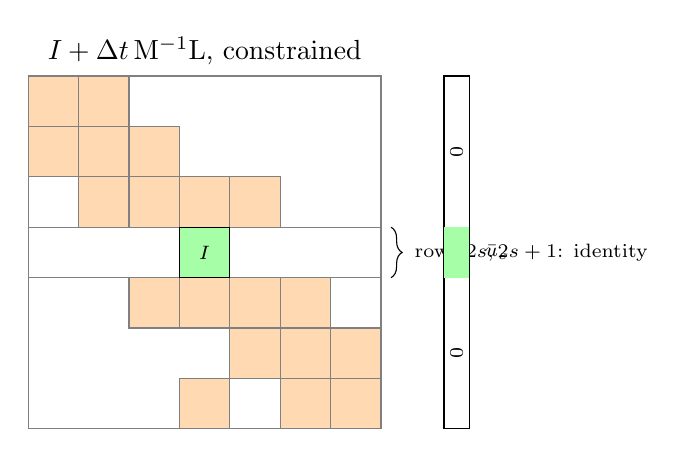
\begin{tikzpicture}[scale=0.32]
  \draw[gray] (0,0) rectangle (14,-14);
  \foreach \i/\j in {0/0,0/2,2/0,2/2,2/4,4/2,4/4,4/8,8/4,8/8,8/10,10/8,10/10,10/12,12/10,12/12,6/6,6/4,4/6,6/8,8/6,6/12,12/6}
    \filldraw[draw=gray, fill=orange!30] (\j,-\i) rectangle ++(2,-2);
  \fill[white] (0,-6) rectangle (14,-8);
  \draw[gray] (0,-6) rectangle (14,-8);
  \filldraw[draw=black, fill=green!35] (6,-6) rectangle ++(2,-2);
  \node[font=\scriptsize] at (7,-7) {$I$};
  \draw[decorate, decoration={brace, amplitude=4pt}] (14.4,-6) -- (14.4,-8) node[midway, right=5pt, font=\scriptsize, align=left] {rows $2s, 2s+1$: identity};
  \draw (16.5,0) rectangle (17.5,-14);
  \fill[green!35] (16.5,-6) rectangle (17.5,-8);
  \node[font=\scriptsize, rotate=90] at (17,-3) {$0$};
  \node[font=\scriptsize, rotate=90] at (17,-11) {$0$};
  \node[font=\scriptsize] at (18.6,-7) {$\bar u_s$};
  \node at (7,1) {$I + \Delta t\, \mathrm M^{-1} \mathrm L$, constrained};
\end{tikzpicture}
}
\caption{The Dirichlet condition by row replacement: the two rows of the source vertex $s$ become rows of the identity, and the right-hand side holds the prescribed vector $\bar u_s$ there and zero elsewhere.}
\label{fig:dirichlet}
\end{figure}

\paragraph{The unit square, finished.} Put the source at vertex $1$ of Example~\ref{ex:s1b_square}, with the prescribed vector $\bar u$ (in the code, $\bar u = (-\frac12, \frac{\sqrt 3}{2})$). Each coordinate is a separate scalar problem with the same matrix, so write $\bar u$ for one coordinate of the source vector and $u_1, \ldots, u_4$ for the same coordinate at the four vertices. \code{PreFactor} replaces the row of vertex $1$ by the row $(1, 0, 0, 0)$ of the identity, and the right-hand side is $\bar u$ in that row and $0$ elsewhere. With the scaled rows computed above, the system is
\begin{align*}
u_1 &= \bar u , \\
-3u_1 + 7u_2 - 3u_3 &= 0 , \\
-\tfrac32 u_2 + 4u_3 - \tfrac32 u_4 &= 0 , \\
-3u_1 - 3u_3 + 7u_4 &= 0 .
\end{align*}
Substitute the first equation, $u_1 = \bar u$, into the second and the fourth, and move the known term to the right:
\begin{equation*}
7u_2 - 3u_3 = 3\bar u, \qquad 7u_4 - 3u_3 = 3\bar u .
\end{equation*}
Subtracting the second of these from the first gives $7u_2 - 7u_4 = 0$, so $u_2 = u_4$, as the symmetry of the square about its diagonal requires. Substitute $u_4 = u_2$ into the third equation and collect:
\begin{align*}
-\tfrac32 u_2 + 4u_3 - \tfrac32 u_2 &= 0 \\
-3u_2 + 4u_3 &= 0 \quad \text{(collect the } u_2 \text{ terms)}\\
u_3 &= \tfrac34\, u_2 .
\end{align*}
Substitute $u_3 = \frac34 u_2$, in parentheses, into $7u_2 - 3u_3 = 3\bar u$:
\begin{align*}
7u_2 - 3\big(\tfrac34 u_2\big) &= 3\bar u \\
\big(\tfrac{28}{4} - \tfrac{9}{4}\big)\, u_2 &= 3\bar u \quad \text{(collect)}\\
\tfrac{19}{4}\, u_2 &= 3\bar u \\
u_2 &= \tfrac{12}{19}\,\bar u .
\end{align*}
Then $u_4 = u_2 = \frac{12}{19}\bar u$ and $u_3 = \frac34\cdot\frac{12}{19}\bar u = \frac{9}{19}\bar u$. As a check, the third equation gives $\frac{1}{19}\big(-\frac32\cdot 12 + 4\cdot 9 - \frac32\cdot 12\big)\bar u = \frac{-18 + 36 - 18}{19}\bar u = 0$. So
\begin{equation*}
u_1 = \bar u, \qquad u_2 = u_4 = \tfrac{12}{19}\,\bar u \approx 0.632\,\bar u, \qquad u_3 = \tfrac{9}{19}\,\bar u \approx 0.474\,\bar u ,
\end{equation*}
for each of the two coordinates, so the vector at every vertex is a positive multiple of the source vector $\bar u$. That is the right answer: on a flat mesh with a common frame, parallel transport does not turn a vector, and the normalization described below would draw the same unit vector at all four vertices. The magnitudes decrease with the distance from the source, the screening of~(\ref{eqn:dirichlet_problem})~[\,$U + \Delta t\,\nabla^*\nabla U = 0 \text{ off } s,\ U(s) = U_s$\,].


\subsection{The calls in \code{main}}

The whole computation of Sections~\ref{section:element}--\ref{section:solve} is a handful of lines of \code{main}:
\lstinputlisting[firstline=638, lastline=645, firstnumber=638]{../src/FEM.cpp}
Line~638 assembles $\Delta t\,\mathrm L$ with $\Delta t = \bar h^2$ (with the option \code{--intrinsic} it calls instead the assembly of Part~\ref{part:intrinsic} written in this part's matrices, Section~\ref{section:int_matrix}); lines~639--640 assemble the lumped $\mathrm M$; line~641 turns \code{A} into $I + \Delta t\,\mathrm M^{-1}\mathrm L$; line~643 replaces the rows of the source and factors; and line~645 solves the system for the right-hand side built above, storing $\mathrm u$ in \code{solutionU}. The program then enters the drawing loop, and the drawing function reads \code{solutionU}.

\subsection{From the solution to vectors}

The solve returns $\mathrm u$, two coordinates per vertex. Its magnitudes decay away from the source; its directions are the transported source vector. So the code keeps only the direction. It reads $u_i$ as the complex number $u_{i,1} + \mathrm i u_{i,2}$, normalizes it, $\hat u_i = u_i / |u_i|$, which needs $u_i \neq 0$ (far from the source $u_i$ is tiny, but not zero), takes its angle $\alpha_i = \arg \hat u_i$, and rotates the first frame vector $t_i$ by $\alpha_i$ about the vertex normal $n_i$. A rotation by the angle $\alpha$ about a unit axis $n$ takes a vector $t$ to $\cos\alpha\, t + \sin\alpha\, n\times t + (1 - \cos\alpha)(n\cdot t)\, n$ (Rodrigues' formula). With $n = n_i$ and $t = t_i$, which is orthogonal to $n_i$:
\begin{align*}
&\cos \alpha_i\, t_i + \sin \alpha_i\, n_i\times t_i + (1 - \cos\alpha_i)(n_i\cdot t_i)\, n_i \\
&= \cos \alpha_i\, t_i + \sin \alpha_i\, n_i\times t_i \quad (n_i\cdot t_i = 0)\\
&= \cos\alpha_i\, t_i + \sin\alpha_i\, b_i \quad (b_i = n_i\times t_i)\\
&= T_i \begin{pmatrix}\cos\alpha_i \\ \sin\alpha_i\end{pmatrix} = T_i\hat u_i \quad (T_i = [\,t_i\;\;b_i\,]) ,
\end{align*}
the tangent vector whose coordinates are $\hat u_i = (\cos\alpha_i, \sin\alpha_i)$. That vector is drawn as an arrow at the vertex, in \code{display}:
\lstinputlisting[firstline=769, lastline=777, firstnumber=769]{../src/FEM.cpp}
Line~771 forms the complex number $u_{i,1} + \mathrm i\, u_{i,2}$ from the entries $2i$ and $2i+1$ of the solution, and line~772 normalizes it to $\hat u_i$. Line~773 recomputes the frame vector $t_i$ exactly as line~185 of \code{computeVertexTangentSpace} did, from the same neighbor. Line~774 builds the rotation about $n_i$ by the angle $\alpha_i$: the complex logarithm of a unit complex number $e^{\mathrm i\alpha}$ is $\mathrm i\alpha$, so \code{log(R\_i).imag()} is $\alpha_i$. Line~775 applies the rotation to $t_i$, giving $T_i\hat u_i$ (or, with \code{--intrinsic}, calls \code{intrinsic::lift} of Part~\ref{part:intrinsic}), and scales it to the length $0.06$ for display; line~776 draws the arrow at the vertex position $x_i$.

\subsection{What the program computes}

Figure~\ref{fig:cactus} shows the result on the cactus that \code{FEM.cpp} loads: one vector prescribed at one vertex has been spread over the whole surface, following its arms and trunk. To see that the directions are right we need a surface where parallel transport is known exactly.

\begin{example}
\label{ex:sphere}
On the unit sphere, the geodesics from a point $s$ are the great circles through it, and transporting a vector along the great circle from $s$ to $x$ is the smallest rotation taking $s$ to $x$, applied to the vector: the rolling of Section~\ref{section:ga_intrinsic}, with the normal turning from $s$ to $x$ in their common plane. The program \code{ga\_fem} solves the problem of this text on a geodesic sphere of $2{,}562$ vertices (an icosahedron subdivided four times, mean edge length $0.076$), with the source at its top vertex, and compares the direction of the result at every vertex with that exact transport (Figure~\ref{fig:sphere}). Out to three quarters of the way to the antipode, the angle between the two is $0.07^\circ$ on average and $0.30^\circ$ at most. Near the antipode the error grows without bound, and it must: every great circle from $s$ reaches the antipode, each with a different transported vector, so there is no shortest path and no correct answer there. The magnitude $|u_i|$ decays by twenty orders of magnitude from the source to the antipode, the screening of~(\ref{eqn:dirichlet_problem})~[\,$U + \Delta t\,\nabla^*\nabla U = 0 \text{ off } s,\ U(s) = U_s$\,] over a distance of order $\sqrt{\Delta t} = \bar h$, and yet the direction, which is all we keep, is accurate wherever it is defined.
\end{example}

\paragraph{What Stage 8 produced.} The global sparse matrices, assembled from the element matrices; the source condition, imposed by replacing the two rows of the source vertex, which is the discrete form of testing only with fields that vanish at $s$ (Stage 4); the solution $\mathrm u$ of the linear system by one sparse LU factorization; and, read back with the vertex frames of Stage 5, a unit tangent vector at every vertex: the source vector transported over the surface.

\begin{figure}[t]
\centering
\adjustbox{max width=\linewidth}{% generated by make_figures.py
\begin{tikzpicture}[]
\filldraw[draw=gray!45, fill=gray!40, line width=0.1pt] (0.2564,-2.5316) -- (0.4139,-2.5100) -- (0.4650,-2.4264) -- cycle;
\filldraw[draw=gray!45, fill=gray!40, line width=0.1pt] (0.4243,-1.8954) -- (0.4778,-1.7312) -- (0.4331,-1.8464) -- cycle;
\filldraw[draw=gray!45, fill=gray!40, line width=0.1pt] (0.4778,-1.7312) -- (0.4705,-1.5366) -- (0.4331,-1.8464) -- cycle;
\filldraw[draw=gray!52, fill=gray!33, line width=0.1pt] (-0.0498,-2.5590) -- (-0.2326,-2.2825) -- (-0.1948,-2.5128) -- cycle;
\filldraw[draw=gray!45, fill=gray!40, line width=0.1pt] (0.4650,-2.4264) -- (0.2460,-2.4590) -- (0.2564,-2.5316) -- cycle;
\filldraw[draw=gray!67, fill=gray!18, line width=0.1pt] (-0.2557,-1.8404) -- (-0.1964,-1.8672) -- (-0.2513,-1.6092) -- cycle;
\filldraw[draw=gray!45, fill=gray!40, line width=0.1pt] (0.4650,-2.4264) -- (0.5010,-2.1123) -- (0.4196,-2.1079) -- cycle;
\filldraw[draw=gray!68, fill=gray!17, line width=0.1pt] (-0.1964,-1.8672) -- (-0.2557,-1.8404) -- (-0.2326,-2.2825) -- cycle;
\filldraw[draw=gray!51, fill=gray!34, line width=0.1pt] (-0.2326,-2.2825) -- (-0.0498,-2.5590) -- (0.0225,-2.5538) -- cycle;
\filldraw[draw=gray!45, fill=gray!40, line width=0.1pt] (0.0225,-2.5538) -- (0.2564,-2.5316) -- (0.1371,-2.5158) -- cycle;
\filldraw[draw=gray!63, fill=gray!22, line width=0.1pt] (-0.2513,-1.6092) -- (-0.1975,-1.5410) -- (-0.2656,-1.4228) -- cycle;
\filldraw[draw=gray!45, fill=gray!40, line width=0.1pt] (0.2564,-2.5316) -- (0.2460,-2.4590) -- (0.1371,-2.5158) -- cycle;
\filldraw[draw=gray!65, fill=gray!20, line width=0.1pt] (-0.2705,-1.2860) -- (-0.2656,-1.4228) -- (-0.2583,-1.2561) -- cycle;
\filldraw[draw=gray!45, fill=gray!40, line width=0.1pt] (0.4196,-2.1079) -- (0.3093,-2.3198) -- (0.4650,-2.4264) -- cycle;
\filldraw[draw=gray!45, fill=gray!40, line width=0.1pt] (0.3093,-2.3198) -- (0.2460,-2.4590) -- (0.4650,-2.4264) -- cycle;
\filldraw[draw=gray!45, fill=gray!40, line width=0.1pt] (0.5087,-1.1630) -- (0.4930,-1.0463) -- (0.4970,-1.0788) -- cycle;
\filldraw[draw=gray!67, fill=gray!18, line width=0.1pt] (-0.2705,-1.2860) -- (-0.2583,-1.2561) -- (-0.2691,-1.2093) -- cycle;
\filldraw[draw=gray!72, fill=gray!13, line width=0.1pt] (-0.2691,-1.2093) -- (-0.2433,-1.1630) -- (-0.2493,-1.1129) -- cycle;
\filldraw[draw=gray!45, fill=gray!40, line width=0.1pt] (0.4970,-1.0788) -- (0.5095,-1.3994) -- (0.5087,-1.1630) -- cycle;
\filldraw[draw=gray!54, fill=gray!31, line width=0.1pt] (-0.1131,-2.2789) -- (-0.2326,-2.2825) -- (0.0225,-2.5538) -- cycle;
\filldraw[draw=gray!45, fill=gray!40, line width=0.1pt] (0.4196,-2.1079) -- (0.5010,-2.1123) -- (0.3938,-1.9714) -- cycle;
\filldraw[draw=gray!63, fill=gray!22, line width=0.1pt] (-0.2493,-1.1129) -- (-0.2433,-1.1630) -- (-0.2646,-0.9518) -- cycle;
\filldraw[draw=gray!45, fill=gray!40, line width=0.1pt] (0.3938,-1.9714) -- (0.5010,-2.1123) -- (0.4331,-1.8464) -- cycle;
\filldraw[draw=gray!67, fill=gray!18, line width=0.1pt] (-0.1964,-1.8672) -- (-0.1975,-1.5410) -- (-0.2513,-1.6092) -- cycle;
\filldraw[draw=gray!64, fill=gray!21, line width=0.1pt] (-0.1131,-2.2789) -- (-0.1964,-1.8672) -- (-0.2326,-2.2825) -- cycle;
\filldraw[draw=gray!45, fill=gray!40, line width=0.1pt] (0.1371,-2.5158) -- (0.0403,-2.4686) -- (0.0225,-2.5538) -- cycle;
\filldraw[draw=gray!63, fill=gray!22, line width=0.1pt] (-0.2583,-1.2561) -- (-0.2656,-1.4228) -- (-0.1975,-1.5410) -- cycle;
\filldraw[draw=gray!54, fill=gray!31, line width=0.1pt] (-0.1131,-2.2789) -- (0.0225,-2.5538) -- (0.0403,-2.4686) -- cycle;
\filldraw[draw=gray!45, fill=gray!40, line width=0.1pt] (0.4985,-1.5856) -- (0.5095,-1.3994) -- (0.3411,-1.5330) -- cycle;
\filldraw[draw=gray!64, fill=gray!21, line width=0.1pt] (-0.2646,-0.9518) -- (-0.2433,-1.1630) -- (-0.2723,-0.8014) -- cycle;
\filldraw[draw=gray!53, fill=gray!32, line width=0.1pt] (0.2460,-2.4590) -- (0.0403,-2.4686) -- (0.1371,-2.5158) -- cycle;
\filldraw[draw=gray!57, fill=gray!28, line width=0.1pt] (-0.1131,-2.2789) -- (0.0403,-2.4686) -- (0.2460,-2.4590) -- cycle;
\filldraw[draw=gray!69, fill=gray!16, line width=0.1pt] (-0.2583,-1.2561) -- (-0.2433,-1.1630) -- (-0.2691,-1.2093) -- cycle;
\filldraw[draw=gray!45, fill=gray!40, line width=0.1pt] (0.4331,-1.8464) -- (0.4985,-1.5856) -- (0.4167,-1.6857) -- cycle;
\filldraw[draw=gray!45, fill=gray!40, line width=0.1pt] (0.4970,-1.0788) -- (0.5067,-0.8861) -- (0.5088,-0.6858) -- cycle;
\filldraw[draw=gray!45, fill=gray!40, line width=0.1pt] (0.3093,-2.3198) -- (0.2684,-2.2885) -- (0.2460,-2.4590) -- cycle;
\filldraw[draw=gray!45, fill=gray!40, line width=0.1pt] (0.3093,-2.3198) -- (0.4196,-2.1079) -- (0.2464,-2.1794) -- cycle;
\filldraw[draw=gray!45, fill=gray!40, line width=0.1pt] (0.4970,-1.0788) -- (0.3411,-1.5330) -- (0.5095,-1.3994) -- cycle;
\filldraw[draw=gray!49, fill=gray!36, line width=0.1pt] (0.2460,-2.4590) -- (0.1194,-2.2162) -- (-0.1131,-2.2789) -- cycle;
\filldraw[draw=gray!45, fill=gray!40, line width=0.1pt] (0.3746,-1.8106) -- (0.3938,-1.9714) -- (0.4331,-1.8464) -- cycle;
\filldraw[draw=gray!45, fill=gray!40, line width=0.1pt] (0.2002,-2.0272) -- (0.4196,-2.1079) -- (0.3938,-1.9714) -- cycle;
\filldraw[draw=gray!46, fill=gray!39, line width=0.1pt] (0.2460,-2.4590) -- (0.2684,-2.2885) -- (0.1194,-2.2162) -- cycle;
\filldraw[draw=gray!45, fill=gray!40, line width=0.1pt] (0.2684,-2.2885) -- (0.3093,-2.3198) -- (0.2464,-2.1794) -- cycle;
\filldraw[draw=gray!62, fill=gray!23, line width=0.1pt] (-0.1964,-1.8672) -- (-0.1131,-2.2789) -- (0.0006,-2.0348) -- cycle;
\filldraw[draw=gray!45, fill=gray!40, line width=0.1pt] (0.4167,-1.6857) -- (0.3746,-1.8106) -- (0.4331,-1.8464) -- cycle;
\filldraw[draw=gray!45, fill=gray!40, line width=0.1pt] (0.4167,-1.6857) -- (0.4985,-1.5856) -- (0.3411,-1.5330) -- cycle;
\filldraw[draw=gray!45, fill=gray!40, line width=0.1pt] (0.4196,-2.1079) -- (0.2002,-2.0272) -- (0.2464,-2.1794) -- cycle;
\filldraw[draw=gray!66, fill=gray!19, line width=0.1pt] (-0.2539,-0.8382) -- (-0.2748,-0.4975) -- (-0.2723,-0.8014) -- cycle;
\filldraw[draw=gray!66, fill=gray!19, line width=0.1pt] (-0.2723,-0.8014) -- (-0.2433,-1.1630) -- (-0.2539,-0.8382) -- cycle;
\filldraw[draw=gray!54, fill=gray!31, line width=0.1pt] (0.0006,-2.0348) -- (-0.1131,-2.2789) -- (0.1194,-2.2162) -- cycle;
\filldraw[draw=gray!45, fill=gray!40, line width=0.1pt] (0.2464,-2.1794) -- (0.1194,-2.2162) -- (0.2684,-2.2885) -- cycle;
\filldraw[draw=gray!45, fill=gray!40, line width=0.1pt] (0.3938,-1.9714) -- (0.3746,-1.8106) -- (0.2002,-2.0272) -- cycle;
\filldraw[draw=gray!45, fill=gray!40, line width=0.1pt] (0.5088,-0.6858) -- (0.5079,-0.5854) -- (0.4872,-0.4723) -- cycle;
\filldraw[draw=gray!52, fill=gray!33, line width=0.1pt] (0.0006,-2.0348) -- (0.1194,-2.2162) -- (0.2464,-2.1794) -- cycle;
\filldraw[draw=gray!52, fill=gray!33, line width=0.1pt] (-0.8161,0.5980) -- (-0.8174,0.5915) -- (-0.6164,0.4472) -- cycle;
\filldraw[draw=gray!66, fill=gray!19, line width=0.1pt] (0.1281,-1.9197) -- (-0.1964,-1.8672) -- (0.0006,-2.0348) -- cycle;
\filldraw[draw=gray!45, fill=gray!40, line width=0.1pt] (0.3411,-1.5330) -- (0.3746,-1.8106) -- (0.4167,-1.6857) -- cycle;
\filldraw[draw=gray!50, fill=gray!35, line width=0.1pt] (0.2464,-2.1794) -- (0.2002,-2.0272) -- (0.0006,-2.0348) -- cycle;
\filldraw[draw=gray!60, fill=gray!25, line width=0.1pt] (0.1025,-1.6464) -- (-0.1975,-1.5410) -- (-0.1964,-1.8672) -- cycle;
\filldraw[draw=gray!47, fill=gray!38, line width=0.1pt] (-1.2450,0.5501) -- (-1.3538,0.6963) -- (-1.3035,0.6250) -- cycle;
\filldraw[draw=gray!45, fill=gray!40, line width=0.1pt] (0.3746,-1.8106) -- (0.2445,-1.8021) -- (0.2002,-2.0272) -- cycle;
\filldraw[draw=gray!68, fill=gray!17, line width=0.1pt] (-0.2583,-1.2561) -- (-0.1975,-1.5410) -- (-0.0692,-1.3132) -- cycle;
\filldraw[draw=gray!61, fill=gray!24, line width=0.1pt] (-0.2583,-1.2561) -- (-0.0692,-1.3132) -- (-0.2433,-1.1630) -- cycle;
\filldraw[draw=gray!76, fill=gray!9, line width=0.1pt] (-0.2539,0.5580) -- (-0.3589,0.4044) -- (-0.3224,0.4550) -- cycle;
\filldraw[draw=gray!59, fill=gray!26, line width=0.1pt] (0.1281,-1.9197) -- (0.1025,-1.6464) -- (-0.1964,-1.8672) -- cycle;
\filldraw[draw=gray!50, fill=gray!35, line width=0.1pt] (0.2002,-2.0272) -- (0.1281,-1.9197) -- (0.0006,-2.0348) -- cycle;
\filldraw[draw=gray!45, fill=gray!40, line width=0.1pt] (0.3411,-1.5330) -- (0.4970,-1.0788) -- (0.3864,-1.2012) -- cycle;
\filldraw[draw=gray!48, fill=gray!37, line width=0.1pt] (-0.8161,0.5980) -- (-0.8966,0.6727) -- (-0.8174,0.5915) -- cycle;
\filldraw[draw=gray!45, fill=gray!40, line width=0.1pt] (0.2445,-1.8021) -- (0.3746,-1.8106) -- (0.3411,-1.5330) -- cycle;
\filldraw[draw=gray!52, fill=gray!33, line width=0.1pt] (-0.6962,0.4995) -- (-0.6164,0.4472) -- (-0.8174,0.5915) -- cycle;
\filldraw[draw=gray!45, fill=gray!40, line width=0.1pt] (-0.8997,0.2548) -- (-0.9221,0.2381) -- (-0.7445,0.1435) -- cycle;
\filldraw[draw=gray!45, fill=gray!40, line width=0.1pt] (0.5088,-0.6858) -- (0.3093,-0.8245) -- (0.4970,-1.0788) -- cycle;
\filldraw[draw=gray!49, fill=gray!36, line width=0.1pt] (0.1281,-1.9197) -- (0.2002,-2.0272) -- (0.2445,-1.8021) -- cycle;
\filldraw[draw=gray!68, fill=gray!17, line width=0.1pt] (-0.2212,-0.6519) -- (-0.2748,-0.4975) -- (-0.2539,-0.8382) -- cycle;
\filldraw[draw=gray!67, fill=gray!18, line width=0.1pt] (-0.1932,-0.9035) -- (-0.2539,-0.8382) -- (-0.2433,-1.1630) -- cycle;
\filldraw[draw=gray!45, fill=gray!40, line width=0.1pt] (-0.8997,0.2548) -- (-0.7445,0.1435) -- (-0.6106,0.0780) -- cycle;
\filldraw[draw=gray!50, fill=gray!35, line width=0.1pt] (-1.2885,0.6367) -- (-1.2450,0.5501) -- (-1.1971,0.4823) -- cycle;
\filldraw[draw=gray!69, fill=gray!16, line width=0.1pt] (-0.5628,0.4479) -- (-0.4750,0.4169) -- (-0.4109,0.4213) -- cycle;
\filldraw[draw=gray!45, fill=gray!40, line width=0.1pt] (-0.3742,0.0330) -- (-0.4852,0.0173) -- (-0.3926,-0.0165) -- cycle;
\filldraw[draw=gray!46, fill=gray!39, line width=0.1pt] (-1.2450,0.5501) -- (-1.2885,0.6367) -- (-1.3538,0.6963) -- cycle;
\filldraw[draw=gray!50, fill=gray!35, line width=0.1pt] (-0.9395,0.7174) -- (-0.9025,0.6538) -- (-0.8966,0.6727) -- cycle;
\filldraw[draw=gray!45, fill=gray!40, line width=0.1pt] (-1.0639,0.9325) -- (-1.0209,0.7887) -- (-0.9395,0.7174) -- cycle;
\filldraw[draw=gray!62, fill=gray!23, line width=0.1pt] (-0.6453,0.4708) -- (-0.4750,0.4169) -- (-0.5628,0.4479) -- cycle;
\draw[-{Stealth[length=2.2mm]}, -{Stealth[length=1.2mm]}, red!75!black, line width=0.45pt] (0.0006,-2.0348) -- (0.1400,-1.9990);
\filldraw[draw=gray!49, fill=gray!36, line width=0.1pt] (0.1281,-1.9197) -- (0.2445,-1.8021) -- (0.1025,-1.6464) -- cycle;
\filldraw[draw=gray!45, fill=gray!40, line width=0.1pt] (-0.9221,0.2381) -- (-0.9825,0.3361) -- (-1.1048,0.3912) -- cycle;
\filldraw[draw=gray!49, fill=gray!36, line width=0.1pt] (0.2445,-1.8021) -- (0.3411,-1.5330) -- (0.1025,-1.6464) -- cycle;
\draw[-{Stealth[length=2.2mm]}, -{Stealth[length=1.2mm]}, red!75!black, line width=0.45pt] (-1.4823,1.1170) -- (-1.3981,1.0359);
\filldraw[draw=gray!53, fill=gray!32, line width=0.1pt] (-0.9025,0.6538) -- (-0.8174,0.5915) -- (-0.8966,0.6727) -- cycle;
\draw[-{Stealth[length=2.2mm]}, -{Stealth[length=1.2mm]}, red!75!black, line width=0.45pt] (0.5011,0.2379) -- (0.5027,0.3170);
\filldraw[draw=gray!59, fill=gray!26, line width=0.1pt] (-0.1975,-1.5410) -- (0.1025,-1.6464) -- (0.0754,-1.4858) -- cycle;
\draw[-{Stealth[length=2.2mm]}, -{Stealth[length=1.2mm]}, red!75!black, line width=0.45pt] (0.2002,-2.0272) -- (0.3354,-1.9703);
\draw[-{Stealth[length=2.2mm]}, -{Stealth[length=1.2mm]}, red!75!black, line width=0.45pt] (-0.9221,0.2381) -- (-0.8095,0.1562);
\draw[-{Stealth[length=2.2mm]}, -{Stealth[length=1.2mm]}, red!75!black, line width=0.45pt] (-1.4023,1.7357) -- (-1.2946,1.6395);
\draw[-{Stealth[length=2.2mm]}, -{Stealth[length=1.2mm]}, red!75!black, line width=0.45pt] (-1.2192,1.4463) -- (-1.1536,1.3332);
\filldraw[draw=gray!45, fill=gray!40, line width=0.1pt] (-1.1834,1.3169) -- (-1.1465,1.1283) -- (-1.1047,1.0188) -- cycle;
\filldraw[draw=gray!45, fill=gray!40, line width=0.1pt] (0.3864,-1.2012) -- (0.4970,-1.0788) -- (0.3093,-0.8245) -- cycle;
\draw[-{Stealth[length=2.2mm]}, -{Stealth[length=1.2mm]}, red!75!black, line width=0.45pt] (-1.4768,1.5352) -- (-1.3999,1.4507);
\draw[-{Stealth[length=2.2mm]}, -{Stealth[length=1.2mm]}, red!75!black, line width=0.45pt] (-0.0183,1.4833) -- (-0.0514,1.6270);
\filldraw[draw=gray!56, fill=gray!29, line width=0.1pt] (0.0754,-1.4858) -- (-0.0692,-1.3132) -- (-0.1975,-1.5410) -- cycle;
\draw[-{Stealth[length=2.2mm]}, -{Stealth[length=1.2mm]}, red!75!black, line width=0.45pt] (-1.2759,1.7136) -- (-1.1909,1.5954);
\draw[-{Stealth[length=2.2mm]}, -{Stealth[length=1.2mm]}, red!75!black, line width=0.45pt] (-0.2539,-0.8382) -- (-0.2165,-0.8215);
\draw[-{Stealth[length=2.2mm]}, -{Stealth[length=1.2mm]}, red!75!black, line width=0.45pt] (-1.0639,0.9325) -- (-0.9970,0.8323);
\filldraw[draw=gray!45, fill=gray!40, line width=0.1pt] (0.4872,-0.4723) -- (0.3093,-0.8245) -- (0.5088,-0.6858) -- cycle;
\filldraw[draw=gray!58, fill=gray!27, line width=0.1pt] (-0.2468,-0.3256) -- (-0.3742,0.0330) -- (-0.3926,-0.0165) -- cycle;
\filldraw[draw=gray!45, fill=gray!40, line width=0.1pt] (-0.9221,0.2381) -- (-0.8997,0.2548) -- (-0.9825,0.3361) -- cycle;
\draw[-{Stealth[length=2.2mm]}, -{Stealth[length=1.2mm]}, red!75!black, line width=0.45pt] (-0.9395,0.7174) -- (-0.8874,0.6156);
\filldraw[draw=gray!45, fill=gray!40, line width=0.1pt] (0.4768,0.0765) -- (0.5011,0.2379) -- (0.3725,0.0273) -- cycle;
\filldraw[draw=gray!51, fill=gray!34, line width=0.1pt] (-1.1796,0.5814) -- (-1.1971,0.4823) -- (-1.1048,0.3912) -- cycle;
\draw[-{Stealth[length=2.2mm]}, -{Stealth[length=1.2mm]}, red!75!black, line width=0.45pt] (-0.2539,0.5580) -- (-0.2894,0.6365);
\filldraw[draw=gray!51, fill=gray!34, line width=0.1pt] (-0.9899,0.7234) -- (-0.9025,0.6538) -- (-0.9395,0.7174) -- cycle;
\draw[-{Stealth[length=2.2mm]}, -{Stealth[length=1.2mm]}, red!75!black, line width=0.45pt] (0.4505,1.0219) -- (0.3403,0.9522);
\draw[-{Stealth[length=2.2mm]}, -{Stealth[length=1.2mm]}, red!75!black, line width=0.45pt] (-1.1834,1.3169) -- (-1.1124,1.2048);
\draw[-{Stealth[length=2.2mm]}, -{Stealth[length=1.2mm]}, red!75!black, line width=0.45pt] (-1.1971,0.4823) -- (-1.1206,0.3769);
\filldraw[draw=gray!79, fill=gray!6, line width=0.1pt] (-0.3442,0.3913) -- (-0.3224,0.4550) -- (-0.4109,0.4213) -- cycle;
\filldraw[draw=gray!66, fill=gray!19, line width=0.1pt] (-0.2212,-0.6519) -- (-0.2539,-0.8382) -- (-0.1932,-0.9035) -- cycle;
\draw[-{Stealth[length=2.2mm]}, -{Stealth[length=1.2mm]}, red!75!black, line width=0.45pt] (-0.8966,0.6727) -- (-0.8149,0.5952);
\filldraw[draw=gray!64, fill=gray!21, line width=0.1pt] (-0.6453,0.4708) -- (-0.5669,0.4090) -- (-0.4750,0.4169) -- cycle;
\draw[-{Stealth[length=2.2mm]}, -{Stealth[length=1.2mm]}, red!75!black, line width=0.45pt] (0.3408,1.4187) -- (0.2225,1.3444);
\draw[-{Stealth[length=2.2mm]}, -{Stealth[length=1.2mm]}, red!75!black, line width=0.45pt] (-0.5628,0.4479) -- (-0.4731,0.4453);
\filldraw[draw=gray!47, fill=gray!38, line width=0.1pt] (0.1025,-1.6464) -- (0.3411,-1.5330) -- (0.0754,-1.4858) -- cycle;
\filldraw[draw=gray!45, fill=gray!40, line width=0.1pt] (0.2309,-1.3258) -- (0.3411,-1.5330) -- (0.3864,-1.2012) -- cycle;
\filldraw[draw=gray!69, fill=gray!16, line width=0.1pt] (-0.2748,-0.4975) -- (-0.2212,-0.6519) -- (-0.1954,-0.4844) -- cycle;
\filldraw[draw=gray!67, fill=gray!18, line width=0.1pt] (-0.4464,0.3245) -- (-0.4109,0.4213) -- (-0.4750,0.4169) -- cycle;
\filldraw[draw=gray!61, fill=gray!24, line width=0.1pt] (-0.1932,-0.9035) -- (-0.2433,-1.1630) -- (-0.0959,-0.9391) -- cycle;
\filldraw[draw=gray!45, fill=gray!40, line width=0.1pt] (-0.9899,0.7234) -- (-0.9395,0.7174) -- (-1.0209,0.7887) -- cycle;
\draw[-{Stealth[length=2.2mm]}, -{Stealth[length=1.2mm]}, red!75!black, line width=0.45pt] (-0.4109,0.4213) -- (-0.3441,0.4231);
\filldraw[draw=gray!45, fill=gray!40, line width=0.1pt] (-0.6106,0.0780) -- (-0.4852,0.0173) -- (-0.4163,0.1425) -- cycle;
\draw[-{Stealth[length=2.2mm]}, -{Stealth[length=1.2mm]}, red!75!black, line width=0.45pt] (0.1281,-1.9197) -- (0.2693,-1.8800);
\filldraw[draw=gray!63, fill=gray!22, line width=0.1pt] (-0.1954,-0.4844) -- (-0.2468,-0.3256) -- (-0.2748,-0.4975) -- cycle;
\filldraw[draw=gray!53, fill=gray!32, line width=0.1pt] (-0.8473,0.5761) -- (-0.8174,0.5915) -- (-0.9025,0.6538) -- cycle;
\filldraw[draw=gray!45, fill=gray!40, line width=0.1pt] (-1.0639,0.9325) -- (-1.1047,1.0188) -- (-1.1714,0.9437) -- cycle;
\filldraw[draw=gray!59, fill=gray!26, line width=0.1pt] (-0.8174,0.5915) -- (-0.7365,0.4464) -- (-0.6962,0.4995) -- cycle;
\draw[-{Stealth[length=2.2mm]}, -{Stealth[length=1.2mm]}, red!75!black, line width=0.45pt] (-0.4852,0.0173) -- (-0.3741,0.0057);
\filldraw[draw=gray!62, fill=gray!23, line width=0.1pt] (-0.6453,0.4708) -- (-0.6962,0.4995) -- (-0.7365,0.4464) -- cycle;
\draw[-{Stealth[length=2.2mm]}, -{Stealth[length=1.2mm]}, red!75!black, line width=0.45pt] (0.2445,-1.8021) -- (0.3808,-1.7469);
\filldraw[draw=gray!75, fill=gray!10, line width=0.1pt] (-0.3224,0.4550) -- (-0.3442,0.3913) -- (-0.2799,0.5353) -- cycle;
\filldraw[draw=gray!46, fill=gray!39, line width=0.1pt] (-1.0499,0.4076) -- (-1.1048,0.3912) -- (-0.9825,0.3361) -- cycle;
\filldraw[draw=gray!45, fill=gray!40, line width=0.1pt] (0.0754,-1.4858) -- (0.3411,-1.5330) -- (0.2309,-1.3258) -- cycle;
\draw[-{Stealth[length=2.2mm]}, -{Stealth[length=1.2mm]}, red!75!black, line width=0.45pt] (-0.6106,0.0780) -- (-0.4695,0.0377);
\filldraw[draw=gray!45, fill=gray!40, line width=0.1pt] (-1.1834,1.3169) -- (-1.1800,1.4431) -- (-1.1949,1.3429) -- cycle;
\draw[-{Stealth[length=2.2mm]}, -{Stealth[length=1.2mm]}, red!75!black, line width=0.45pt] (0.3411,-1.5330) -- (0.4461,-1.4668);
\filldraw[draw=gray!45, fill=gray!40, line width=0.1pt] (0.5075,-0.0434) -- (0.4768,0.0765) -- (0.3725,0.0273) -- cycle;
\filldraw[draw=gray!68, fill=gray!17, line width=0.1pt] (0.0505,-1.0020) -- (-0.2433,-1.1630) -- (-0.0692,-1.3132) -- cycle;
\filldraw[draw=gray!46, fill=gray!39, line width=0.1pt] (-1.2885,0.6367) -- (-1.1971,0.4823) -- (-1.1796,0.5814) -- cycle;
\draw[-{Stealth[length=2.2mm]}, -{Stealth[length=1.2mm]}, red!75!black, line width=0.45pt] (-1.1048,0.3912) -- (-1.0159,0.2842);
\draw[-{Stealth[length=2.2mm]}, -{Stealth[length=1.2mm]}, red!75!black, line width=0.45pt] (-1.2135,1.6264) -- (-1.1520,1.5042);
\draw[-{Stealth[length=2.2mm]}, -{Stealth[length=1.2mm]}, red!75!black, line width=0.45pt] (-1.4299,1.8898) -- (-1.3284,1.7846);
\draw[-{Stealth[length=2.2mm]}, -{Stealth[length=1.2mm]}, red!75!black, line width=0.45pt] (-1.3538,0.6963) -- (-1.3146,0.5839);
\draw[-{Stealth[length=2.2mm]}, -{Stealth[length=1.2mm]}, red!75!black, line width=0.45pt] (-0.2478,0.6634) -- (-0.2884,0.7422);
\filldraw[draw=gray!45, fill=gray!40, line width=0.1pt] (-0.6106,0.0780) -- (-0.7304,0.2570) -- (-0.8997,0.2548) -- cycle;
\draw[-{Stealth[length=2.2mm]}, -{Stealth[length=1.2mm]}, red!75!black, line width=0.45pt] (-0.1456,1.3141) -- (-0.2037,1.4378);
\draw[-{Stealth[length=2.2mm]}, -{Stealth[length=1.2mm]}, red!75!black, line width=0.45pt] (-0.3224,0.4550) -- (-0.2769,0.4946);
\filldraw[draw=gray!45, fill=gray!40, line width=0.1pt] (-1.1465,1.1283) -- (-1.1429,1.0678) -- (-1.1047,1.0188) -- cycle;
\filldraw[draw=gray!58, fill=gray!27, line width=0.1pt] (-1.3447,0.9248) -- (-1.4607,0.9313) -- (-1.3538,0.6963) -- cycle;
\filldraw[draw=gray!52, fill=gray!33, line width=0.1pt] (-0.7365,0.4464) -- (-0.8174,0.5915) -- (-0.8473,0.5761) -- cycle;
\filldraw[draw=gray!64, fill=gray!21, line width=0.1pt] (-0.5669,0.4090) -- (-0.6453,0.4708) -- (-0.7365,0.4464) -- cycle;
\draw[-{Stealth[length=2.2mm]}, -{Stealth[length=1.2mm]}, red!75!black, line width=0.45pt] (-1.1047,1.0188) -- (-1.0704,0.8989);
\filldraw[draw=gray!45, fill=gray!40, line width=0.1pt] (-1.1834,1.3169) -- (-1.1949,1.3429) -- (-1.1640,1.2554) -- cycle;
\filldraw[draw=gray!46, fill=gray!39, line width=0.1pt] (-1.0209,0.7887) -- (-1.0639,0.9325) -- (-1.1714,0.9437) -- cycle;
\filldraw[draw=gray!65, fill=gray!20, line width=0.1pt] (-0.4464,0.3245) -- (-0.4750,0.4169) -- (-0.5669,0.4090) -- cycle;
\draw[-{Stealth[length=2.2mm]}, -{Stealth[length=1.2mm]}, red!75!black, line width=0.45pt] (-0.4750,0.4169) -- (-0.3942,0.3347);
\filldraw[draw=gray!50, fill=gray!35, line width=0.1pt] (-1.1048,0.3912) -- (-1.0499,0.4076) -- (-1.1796,0.5814) -- cycle;
\draw[-{Stealth[length=2.2mm]}, -{Stealth[length=1.2mm]}, red!75!black, line width=0.45pt] (-0.8174,0.5915) -- (-0.7330,0.4973);
\filldraw[draw=gray!79, fill=gray!6, line width=0.1pt] (-0.4464,0.3245) -- (-0.3442,0.3913) -- (-0.4109,0.4213) -- cycle;
\filldraw[draw=gray!52, fill=gray!33, line width=0.1pt] (0.0505,-1.0020) -- (-0.0959,-0.9391) -- (-0.2433,-1.1630) -- cycle;
\draw[-{Stealth[length=2.2mm]}, -{Stealth[length=1.2mm]}, red!75!black, line width=0.45pt] (-1.4607,0.9313) -- (-1.4407,0.8225);
\draw[-{Stealth[length=2.2mm]}, -{Stealth[length=1.2mm]}, red!75!black, line width=0.45pt] (0.0737,1.8720) -- (0.1333,2.0081);
\draw[-{Stealth[length=2.2mm]}, -{Stealth[length=1.2mm]}, red!75!black, line width=0.45pt] (-1.2339,1.8271) -- (-1.1466,1.7055);
\filldraw[draw=gray!58, fill=gray!27, line width=0.1pt] (-0.0692,-1.3132) -- (0.0754,-1.4858) -- (0.2309,-1.3258) -- cycle;
\filldraw[draw=gray!54, fill=gray!31, line width=0.1pt] (-0.3742,0.0330) -- (-0.4163,0.1425) -- (-0.4852,0.0173) -- cycle;
\draw[-{Stealth[length=2.2mm]}, -{Stealth[length=1.2mm]}, red!75!black, line width=0.45pt] (-0.6962,0.4995) -- (-0.6205,0.4139);
\draw[-{Stealth[length=2.2mm]}, -{Stealth[length=1.2mm]}, red!75!black, line width=0.45pt] (0.3864,-1.2012) -- (0.4877,-1.1348);
\draw[-{Stealth[length=2.2mm]}, -{Stealth[length=1.2mm]}, red!75!black, line width=0.45pt] (-1.5004,1.7352) -- (-1.4524,1.6446);
\filldraw[draw=gray!45, fill=gray!40, line width=0.1pt] (-1.2135,1.6264) -- (-1.2244,1.4781) -- (-1.1800,1.4431) -- cycle;
\filldraw[draw=gray!52, fill=gray!33, line width=0.1pt] (-0.8007,0.4332) -- (-0.9825,0.3361) -- (-0.8997,0.2548) -- cycle;
\filldraw[draw=gray!60, fill=gray!25, line width=0.1pt] (-1.3538,0.6963) -- (-1.2885,0.6367) -- (-1.3447,0.9248) -- cycle;
\filldraw[draw=gray!65, fill=gray!20, line width=0.1pt] (-0.8473,0.5761) -- (-0.9025,0.6538) -- (-1.0836,0.5225) -- cycle;
\filldraw[draw=gray!49, fill=gray!36, line width=0.1pt] (-0.9899,0.7234) -- (-1.0836,0.5225) -- (-0.9025,0.6538) -- cycle;
\draw[-{Stealth[length=2.2mm]}, -{Stealth[length=1.2mm]}, red!75!black, line width=0.45pt] (-0.6453,0.4708) -- (-0.5531,0.4030);
\filldraw[draw=gray!45, fill=gray!40, line width=0.1pt] (-0.7304,0.2570) -- (-0.6106,0.0780) -- (-0.6294,0.2316) -- cycle;
\draw[-{Stealth[length=2.2mm]}, -{Stealth[length=1.2mm]}, red!75!black, line width=0.45pt] (0.4872,-0.4723) -- (0.5460,-0.4011);
\draw[-{Stealth[length=2.2mm]}, -{Stealth[length=1.2mm]}, red!75!black, line width=0.45pt] (0.5075,-0.0434) -- (0.5255,0.0265);
\filldraw[draw=gray!79, fill=gray!6, line width=0.1pt] (-0.2799,0.5353) -- (-0.3442,0.3913) -- (-0.3067,0.4394) -- cycle;
\draw[-{Stealth[length=2.2mm]}, -{Stealth[length=1.2mm]}, red!75!black, line width=0.45pt] (0.5361,0.6754) -- (0.4268,0.6608);
\draw[-{Stealth[length=2.2mm]}, -{Stealth[length=1.2mm]}, red!75!black, line width=0.45pt] (-1.2794,2.0367) -- (-1.1788,1.9228);
\filldraw[draw=gray!45, fill=gray!40, line width=0.1pt] (-0.4163,0.1425) -- (-0.6294,0.2316) -- (-0.6106,0.0780) -- cycle;
\filldraw[draw=gray!45, fill=gray!40, line width=0.1pt] (-1.1429,1.0678) -- (-1.1714,0.9437) -- (-1.1047,1.0188) -- cycle;
\filldraw[draw=gray!45, fill=gray!40, line width=0.1pt] (0.2309,-1.3258) -- (0.3864,-1.2012) -- (0.3093,-0.8245) -- cycle;
\draw[-{Stealth[length=2.2mm]}, -{Stealth[length=1.2mm]}, red!75!black, line width=0.45pt] (-0.2513,0.7642) -- (-0.2915,0.8455);
\filldraw[draw=gray!50, fill=gray!35, line width=0.1pt] (-0.9825,0.3361) -- (-0.8007,0.4332) -- (-1.0499,0.4076) -- cycle;
\draw[-{Stealth[length=2.2mm]}, -{Stealth[length=1.2mm]}, red!75!black, line width=0.45pt] (-0.2799,0.5353) -- (-0.2710,0.5950);
\draw[-{Stealth[length=2.2mm]}, -{Stealth[length=1.2mm]}, red!75!black, line width=0.45pt] (-1.2469,1.9676) -- (-1.1700,1.8433);
\filldraw[draw=gray!52, fill=gray!33, line width=0.1pt] (-1.0209,0.7887) -- (-1.0822,0.7115) -- (-0.9899,0.7234) -- cycle;
\draw[-{Stealth[length=2.2mm]}, -{Stealth[length=1.2mm]}, red!75!black, line width=0.45pt] (-1.1800,1.4431) -- (-1.1658,1.3158);
\filldraw[draw=gray!62, fill=gray!23, line width=0.1pt] (-0.7365,0.4464) -- (-0.5418,0.3143) -- (-0.5669,0.4090) -- cycle;
\filldraw[draw=gray!61, fill=gray!24, line width=0.1pt] (-0.7365,0.4464) -- (-0.8473,0.5761) -- (-0.8007,0.4332) -- cycle;
\draw[-{Stealth[length=2.2mm]}, -{Stealth[length=1.2mm]}, red!75!black, line width=0.45pt] (0.1025,-1.6464) -- (0.2438,-1.6065);
\draw[-{Stealth[length=2.2mm]}, -{Stealth[length=1.2mm]}, red!75!black, line width=0.45pt] (-1.4227,2.1137) -- (-1.3300,2.0109);
\draw[-{Stealth[length=2.2mm]}, -{Stealth[length=1.2mm]}, red!75!black, line width=0.45pt] (-0.9025,0.6538) -- (-0.8505,0.5205);
\draw[-{Stealth[length=2.2mm]}, -{Stealth[length=1.2mm]}, red!75!black, line width=0.45pt] (-0.2182,1.1046) -- (-0.2652,1.2087);
\filldraw[draw=gray!62, fill=gray!23, line width=0.1pt] (-0.8997,0.2548) -- (-0.7304,0.2570) -- (-0.8007,0.4332) -- cycle;
\filldraw[draw=gray!50, fill=gray!35, line width=0.1pt] (0.2309,-1.3258) -- (0.1124,-1.1109) -- (-0.0692,-1.3132) -- cycle;
\draw[-{Stealth[length=2.2mm]}, -{Stealth[length=1.2mm]}, red!75!black, line width=0.45pt] (-0.2055,1.2107) -- (-0.2484,1.3214);
\filldraw[draw=gray!63, fill=gray!22, line width=0.1pt] (-1.4607,0.9313) -- (-1.3870,1.2680) -- (-1.5283,1.2834) -- cycle;
\filldraw[draw=gray!69, fill=gray!16, line width=0.1pt] (-0.5418,0.3143) -- (-0.4464,0.3245) -- (-0.5669,0.4090) -- cycle;
\draw[-{Stealth[length=2.2mm]}, -{Stealth[length=1.2mm]}, red!75!black, line width=0.45pt] (-0.2477,0.8769) -- (-0.2981,0.9643);
\filldraw[draw=gray!62, fill=gray!23, line width=0.1pt] (-0.8473,0.5761) -- (-1.0836,0.5225) -- (-0.8007,0.4332) -- cycle;
\filldraw[draw=gray!66, fill=gray!19, line width=0.1pt] (-1.1796,0.5814) -- (-1.0822,0.7115) -- (-1.2885,0.6367) -- cycle;
\filldraw[draw=gray!45, fill=gray!40, line width=0.1pt] (0.5011,0.2379) -- (0.5085,0.3447) -- (0.3725,0.0273) -- cycle;
\filldraw[draw=gray!52, fill=gray!33, line width=0.1pt] (-1.1796,0.5814) -- (-1.0499,0.4076) -- (-1.0836,0.5225) -- cycle;
\filldraw[draw=gray!49, fill=gray!36, line width=0.1pt] (-1.0499,0.4076) -- (-0.8007,0.4332) -- (-1.0836,0.5225) -- cycle;
\filldraw[draw=gray!45, fill=gray!40, line width=0.1pt] (-1.2287,1.1706) -- (-1.1465,1.1283) -- (-1.1640,1.2554) -- cycle;
\filldraw[draw=gray!45, fill=gray!40, line width=0.1pt] (0.3725,0.0273) -- (0.4872,-0.4723) -- (0.5075,-0.0434) -- cycle;
\filldraw[draw=gray!45, fill=gray!40, line width=0.1pt] (-0.9899,0.7234) -- (-1.0822,0.7115) -- (-1.0836,0.5225) -- cycle;
\draw[-{Stealth[length=2.2mm]}, -{Stealth[length=1.2mm]}, red!75!black, line width=0.45pt] (-1.4897,1.9584) -- (-1.4205,1.8654);
\draw[-{Stealth[length=2.2mm]}, -{Stealth[length=1.2mm]}, red!75!black, line width=0.45pt] (0.6595,0.9026) -- (0.5729,0.7867);
\draw[-{Stealth[length=2.2mm]}, -{Stealth[length=1.2mm]}, red!75!black, line width=0.45pt] (-0.8997,0.2548) -- (-0.7779,0.1652);
\filldraw[draw=gray!55, fill=gray!30, line width=0.1pt] (-0.7365,0.4464) -- (-0.8007,0.4332) -- (-0.7304,0.2570) -- cycle;
\draw[-{Stealth[length=2.2mm]}, -{Stealth[length=1.2mm]}, red!75!black, line width=0.45pt] (-0.1932,-0.9035) -- (-0.0935,-0.8836);
\draw[-{Stealth[length=2.2mm]}, -{Stealth[length=1.2mm]}, red!75!black, line width=0.45pt] (-1.5283,1.2834) -- (-1.5178,1.1885);
\filldraw[draw=gray!61, fill=gray!24, line width=0.1pt] (-0.6294,0.2316) -- (-0.5418,0.3143) -- (-0.7365,0.4464) -- cycle;
\filldraw[draw=gray!60, fill=gray!25, line width=0.1pt] (-0.7365,0.4464) -- (-0.7304,0.2570) -- (-0.6294,0.2316) -- cycle;
\draw[-{Stealth[length=2.2mm]}, -{Stealth[length=1.2mm]}, red!75!black, line width=0.45pt] (-0.1653,1.5207) -- (-0.2033,1.6457);
\filldraw[draw=gray!45, fill=gray!40, line width=0.1pt] (-1.1714,0.9437) -- (-1.0822,0.7115) -- (-1.0209,0.7887) -- cycle;
\filldraw[draw=gray!45, fill=gray!40, line width=0.1pt] (-1.1465,1.1283) -- (-1.2287,1.1706) -- (-1.1429,1.0678) -- cycle;
\draw[-{Stealth[length=2.2mm]}, -{Stealth[length=1.2mm]}, red!75!black, line width=0.45pt] (-1.2239,2.0120) -- (-1.1496,1.8865);
\filldraw[draw=gray!65, fill=gray!20, line width=0.1pt] (-0.1932,-0.9035) -- (-0.0695,-0.4623) -- (-0.2212,-0.6519) -- cycle;
\draw[-{Stealth[length=2.2mm]}, -{Stealth[length=1.2mm]}, red!75!black, line width=0.45pt] (-0.5669,0.4090) -- (-0.4621,0.3158);
\draw[-{Stealth[length=2.2mm]}, -{Stealth[length=1.2mm]}, red!75!black, line width=0.45pt] (-0.0692,-1.3132) -- (0.0600,-1.2846);
\filldraw[draw=gray!51, fill=gray!34, line width=0.1pt] (-1.3447,0.9248) -- (-1.2885,0.6367) -- (-1.0822,0.7115) -- cycle;
\filldraw[draw=gray!59, fill=gray!26, line width=0.1pt] (-1.0822,0.7115) -- (-1.1796,0.5814) -- (-1.0836,0.5225) -- cycle;
\draw[-{Stealth[length=2.2mm]}, -{Stealth[length=1.2mm]}, red!75!black, line width=0.45pt] (-1.0209,0.7887) -- (-0.9852,0.6525);
\draw[-{Stealth[length=2.2mm]}, -{Stealth[length=1.2mm]}, red!75!black, line width=0.45pt] (-0.9825,0.3361) -- (-0.8787,0.2292);
\filldraw[draw=gray!54, fill=gray!31, line width=0.1pt] (0.0505,-1.0020) -- (-0.0692,-1.3132) -- (0.1124,-1.1109) -- cycle;
\draw[-{Stealth[length=2.2mm]}, -{Stealth[length=1.2mm]}, red!75!black, line width=0.45pt] (-1.2728,2.2024) -- (-1.1644,2.0968);
\filldraw[draw=gray!59, fill=gray!26, line width=0.1pt] (-0.4163,0.1425) -- (-0.4464,0.3245) -- (-0.5418,0.3143) -- cycle;
\draw[-{Stealth[length=2.2mm]}, -{Stealth[length=1.2mm]}, red!75!black, line width=0.45pt] (0.0754,-1.4858) -- (0.2191,-1.4454);
\filldraw[draw=gray!65, fill=gray!20, line width=0.1pt] (-1.5283,1.2834) -- (-1.5040,1.5009) -- (-1.5348,1.4793) -- cycle;
\draw[-{Stealth[length=2.2mm]}, -{Stealth[length=1.2mm]}, red!75!black, line width=0.45pt] (-0.2212,-0.6519) -- (-0.1439,-0.6365);
\filldraw[draw=gray!45, fill=gray!40, line width=0.1pt] (-1.1800,1.4431) -- (-1.2244,1.4781) -- (-1.1949,1.3429) -- cycle;
\filldraw[draw=gray!59, fill=gray!26, line width=0.1pt] (-0.6294,0.2316) -- (-0.4163,0.1425) -- (-0.5418,0.3143) -- cycle;
\draw[-{Stealth[length=2.2mm]}, -{Stealth[length=1.2mm]}, red!75!black, line width=0.45pt] (-1.2885,0.6367) -- (-1.2540,0.5013);
\draw[-{Stealth[length=2.2mm]}, -{Stealth[length=1.2mm]}, red!75!black, line width=0.45pt] (-0.8473,0.5761) -- (-0.7768,0.4499);
\draw[-{Stealth[length=2.2mm]}, -{Stealth[length=1.2mm]}, red!75!black, line width=0.45pt] (-1.1640,1.2554) -- (-1.1656,1.1189);
\draw[-{Stealth[length=2.2mm]}, -{Stealth[length=1.2mm]}, red!75!black, line width=0.45pt] (-1.2037,1.9493) -- (-1.1727,1.8179);
\filldraw[draw=gray!48, fill=gray!37, line width=0.1pt] (0.2309,-1.3258) -- (0.3093,-0.8245) -- (0.1124,-1.1109) -- cycle;
\draw[-{Stealth[length=2.2mm]}, -{Stealth[length=1.2mm]}, red!75!black, line width=0.45pt] (-0.9899,0.7234) -- (-0.9686,0.5750);
\draw[-{Stealth[length=2.2mm]}, -{Stealth[length=1.2mm]}, red!75!black, line width=0.45pt] (-1.1465,1.1283) -- (-1.1368,0.9938);
\filldraw[draw=gray!45, fill=gray!40, line width=0.1pt] (-1.1949,1.3429) -- (-1.2287,1.1706) -- (-1.1640,1.2554) -- cycle;
\filldraw[draw=gray!61, fill=gray!24, line width=0.1pt] (-0.2358,0.0622) -- (-0.3742,0.0330) -- (-0.2468,-0.3256) -- cycle;
\filldraw[draw=gray!68, fill=gray!17, line width=0.1pt] (-1.5189,1.5649) -- (-1.5367,1.5848) -- (-1.5348,1.4793) -- cycle;
\filldraw[draw=gray!72, fill=gray!13, line width=0.1pt] (-0.2779,0.6115) -- (-0.3067,0.4394) -- (-0.2721,0.5235) -- cycle;
\filldraw[draw=gray!63, fill=gray!22, line width=0.1pt] (-1.3870,1.2680) -- (-1.4607,0.9313) -- (-1.3447,0.9248) -- cycle;
\draw[-{Stealth[length=2.2mm]}, -{Stealth[length=1.2mm]}, red!75!black, line width=0.45pt] (-0.2168,1.3307) -- (-0.2523,1.4441);
\filldraw[draw=gray!64, fill=gray!21, line width=0.1pt] (-0.1932,-0.9035) -- (-0.0959,-0.9391) -- (-0.0695,-0.4623) -- cycle;
\draw[-{Stealth[length=2.2mm]}, -{Stealth[length=1.2mm]}, red!75!black, line width=0.45pt] (-0.0945,1.9134) -- (-0.0941,2.0634);
\filldraw[draw=gray!45, fill=gray!40, line width=0.1pt] (0.4872,-0.4723) -- (0.2622,-0.5238) -- (0.3093,-0.8245) -- cycle;
\draw[-{Stealth[length=2.2mm]}, -{Stealth[length=1.2mm]}, red!75!black, line width=0.45pt] (-1.0499,0.4076) -- (-0.9615,0.2889);
\draw[-{Stealth[length=2.2mm]}, -{Stealth[length=1.2mm]}, red!75!black, line width=0.45pt] (-0.2468,-0.3256) -- (-0.2011,-0.3215);
\draw[-{Stealth[length=2.2mm]}, -{Stealth[length=1.2mm]}, red!75!black, line width=0.45pt] (0.0011,2.1294) -- (0.1065,2.2348);
\draw[-{Stealth[length=2.2mm]}, -{Stealth[length=1.2mm]}, red!75!black, line width=0.45pt] (0.5085,0.3447) -- (0.5452,0.4272);
\draw[-{Stealth[length=2.2mm]}, -{Stealth[length=1.2mm]}, red!75!black, line width=0.45pt] (0.2309,-1.3258) -- (0.3715,-1.2732);
\filldraw[draw=gray!45, fill=gray!40, line width=0.1pt] (-1.1714,0.9437) -- (-1.1429,1.0678) -- (-1.2287,1.1706) -- cycle;
\filldraw[draw=gray!61, fill=gray!24, line width=0.1pt] (-0.2212,-0.6519) -- (-0.0695,-0.4623) -- (-0.1954,-0.4844) -- cycle;
\draw[-{Stealth[length=2.2mm]}, -{Stealth[length=1.2mm]}, red!75!black, line width=0.45pt] (-1.5367,1.5848) -- (-1.5108,1.4883);
\filldraw[draw=gray!78, fill=gray!7, line width=0.1pt] (-0.3442,0.3913) -- (-0.2507,0.3937) -- (-0.3067,0.4394) -- cycle;
\filldraw[draw=gray!54, fill=gray!31, line width=0.1pt] (-0.3742,0.0330) -- (-0.2358,0.0622) -- (-0.4163,0.1425) -- cycle;
\filldraw[draw=gray!63, fill=gray!22, line width=0.1pt] (-1.5367,1.5848) -- (-1.5189,1.5649) -- (-1.5429,1.6741) -- cycle;
\filldraw[draw=gray!53, fill=gray!32, line width=0.1pt] (-1.0822,0.7115) -- (-1.1714,0.9437) -- (-1.3447,0.9248) -- cycle;
\filldraw[draw=gray!79, fill=gray!6, line width=0.1pt] (-0.2507,0.3937) -- (-0.3442,0.3913) -- (-0.4464,0.3245) -- cycle;
\draw[-{Stealth[length=2.2mm]}, -{Stealth[length=1.2mm]}, red!75!black, line width=0.45pt] (-1.1429,1.0678) -- (-1.1536,0.9253);
\draw[-{Stealth[length=2.2mm]}, -{Stealth[length=1.2mm]}, red!75!black, line width=0.45pt] (-0.7365,0.4464) -- (-0.6495,0.3271);
\draw[-{Stealth[length=2.2mm]}, -{Stealth[length=1.2mm]}, red!75!black, line width=0.45pt] (0.8001,0.8435) -- (0.7425,0.7049);
\draw[-{Stealth[length=2.2mm]}, -{Stealth[length=1.2mm]}, red!75!black, line width=0.45pt] (-0.3742,0.0330) -- (-0.2866,0.0249);
\filldraw[draw=gray!61, fill=gray!24, line width=0.1pt] (-0.0959,-0.9391) -- (0.0505,-1.0020) -- (0.1112,-0.8966) -- cycle;
\filldraw[draw=gray!66, fill=gray!19, line width=0.1pt] (-0.4163,0.1425) -- (-0.2507,0.3937) -- (-0.4464,0.3245) -- cycle;
\filldraw[draw=gray!45, fill=gray!40, line width=0.1pt] (-1.1777,1.7694) -- (-1.1991,1.7982) -- (-1.1791,1.6641) -- cycle;
\filldraw[draw=gray!47, fill=gray!38, line width=0.1pt] (0.3093,-0.8245) -- (0.1112,-0.8966) -- (0.1124,-1.1109) -- cycle;
\filldraw[draw=gray!53, fill=gray!32, line width=0.1pt] (0.0505,-1.0020) -- (0.1124,-1.1109) -- (0.1112,-0.8966) -- cycle;
\draw[-{Stealth[length=2.2mm]}, -{Stealth[length=1.2mm]}, red!75!black, line width=0.45pt] (-1.5036,2.1449) -- (-1.4298,2.0440);
\draw[-{Stealth[length=2.2mm]}, -{Stealth[length=1.2mm]}, red!75!black, line width=0.45pt] (-0.3442,0.3913) -- (-0.2473,0.4163);
\draw[-{Stealth[length=2.2mm]}, -{Stealth[length=1.2mm]}, red!75!black, line width=0.45pt] (-0.3067,0.4394) -- (-0.2579,0.4862);
\filldraw[draw=gray!53, fill=gray!32, line width=0.1pt] (-1.1714,0.9437) -- (-1.2287,1.1706) -- (-1.3447,0.9248) -- cycle;
\draw[-{Stealth[length=2.2mm]}, -{Stealth[length=1.2mm]}, red!75!black, line width=0.45pt] (-1.1884,2.0005) -- (-1.1787,1.8673);
\draw[-{Stealth[length=2.2mm]}, -{Stealth[length=1.2mm]}, red!75!black, line width=0.45pt] (-1.1796,0.5814) -- (-1.1252,0.4446);
\draw[-{Stealth[length=2.2mm]}, -{Stealth[length=1.2mm]}, red!75!black, line width=0.45pt] (-1.4718,2.2668) -- (-1.4021,2.1652);
\draw[-{Stealth[length=2.2mm]}, -{Stealth[length=1.2mm]}, red!75!black, line width=0.45pt] (-0.8007,0.4332) -- (-0.7106,0.3108);
\filldraw[draw=gray!60, fill=gray!25, line width=0.1pt] (-1.5283,1.2834) -- (-1.4437,1.4336) -- (-1.5040,1.5009) -- cycle;
\draw[-{Stealth[length=2.2mm]}, -{Stealth[length=1.2mm]}, red!75!black, line width=0.45pt] (-0.2779,0.6115) -- (-0.2722,0.6709);
\draw[-{Stealth[length=2.2mm]}, -{Stealth[length=1.2mm]}, red!75!black, line width=0.45pt] (-1.5348,1.4793) -- (-1.5217,1.3800);
\filldraw[draw=gray!64, fill=gray!21, line width=0.1pt] (-1.5189,1.5649) -- (-1.5348,1.4793) -- (-1.5040,1.5009) -- cycle;
\draw[-{Stealth[length=2.2mm]}, -{Stealth[length=1.2mm]}, red!75!black, line width=0.45pt] (-1.3988,2.3359) -- (-1.3072,2.2607);
\filldraw[draw=gray!69, fill=gray!16, line width=0.1pt] (-0.3067,0.4394) -- (-0.2507,0.3937) -- (-0.2721,0.5235) -- cycle;
\draw[-{Stealth[length=2.2mm]}, -{Stealth[length=1.2mm]}, red!75!black, line width=0.45pt] (-0.4464,0.3245) -- (-0.3104,0.3007);
\filldraw[draw=gray!45, fill=gray!40, line width=0.1pt] (-1.1896,2.1752) -- (-1.1993,2.0251) -- (-1.1884,2.0005) -- cycle;
\draw[-{Stealth[length=2.2mm]}, -{Stealth[length=1.2mm]}, red!75!black, line width=0.45pt] (-0.5418,0.3143) -- (-0.4033,0.2527);
\filldraw[draw=gray!60, fill=gray!25, line width=0.1pt] (-1.3870,1.2680) -- (-1.4437,1.4336) -- (-1.5283,1.2834) -- cycle;
\draw[-{Stealth[length=2.2mm]}, -{Stealth[length=1.2mm]}, red!75!black, line width=0.45pt] (0.4517,1.6622) -- (0.3988,1.5412);
\filldraw[draw=gray!45, fill=gray!40, line width=0.1pt] (-1.2751,1.3098) -- (-1.2287,1.1706) -- (-1.1949,1.3429) -- cycle;
\draw[-{Stealth[length=2.2mm]}, -{Stealth[length=1.2mm]}, red!75!black, line width=0.45pt] (-0.7304,0.2570) -- (-0.5929,0.1924);
\filldraw[draw=gray!68, fill=gray!17, line width=0.1pt] (-0.0376,-0.0861) -- (-0.2468,-0.3256) -- (-0.1954,-0.4844) -- cycle;
\draw[-{Stealth[length=2.2mm]}, -{Stealth[length=1.2mm]}, red!75!black, line width=0.45pt] (0.5194,0.4984) -- (0.5585,0.5895);
\draw[-{Stealth[length=2.2mm]}, -{Stealth[length=1.2mm]}, red!75!black, line width=0.45pt] (-0.0959,-0.9391) -- (0.0333,-0.9096);
\filldraw[draw=gray!57, fill=gray!28, line width=0.1pt] (-0.0695,-0.4623) -- (-0.0959,-0.9391) -- (0.1112,-0.8966) -- cycle;
\draw[-{Stealth[length=2.2mm]}, -{Stealth[length=1.2mm]}, red!75!black, line width=0.45pt] (-1.0836,0.5225) -- (-1.0165,0.3861);
\draw[-{Stealth[length=2.2mm]}, -{Stealth[length=1.2mm]}, red!75!black, line width=0.45pt] (-0.6294,0.2316) -- (-0.4863,0.1811);
\draw[-{Stealth[length=2.2mm]}, -{Stealth[length=1.2mm]}, red!75!black, line width=0.45pt] (-0.2684,0.9380) -- (-0.2999,1.0215);
\draw[-{Stealth[length=2.2mm]}, -{Stealth[length=1.2mm]}, red!75!black, line width=0.45pt] (-1.1791,1.6641) -- (-1.2127,1.5299);
\filldraw[draw=gray!67, fill=gray!18, line width=0.1pt] (-0.2560,0.7733) -- (-0.2743,0.8863) -- (-0.2779,0.6115) -- cycle;
\filldraw[draw=gray!45, fill=gray!40, line width=0.1pt] (-1.1949,1.3429) -- (-1.2244,1.4781) -- (-1.2751,1.3098) -- cycle;
\filldraw[draw=gray!45, fill=gray!40, line width=0.1pt] (0.4872,-0.4723) -- (0.2327,-0.2574) -- (0.2622,-0.5238) -- cycle;
\draw[-{Stealth[length=2.2mm]}, -{Stealth[length=1.2mm]}, red!75!black, line width=0.45pt] (-1.2778,2.3067) -- (-1.1635,2.2067);
\draw[-{Stealth[length=2.2mm]}, -{Stealth[length=1.2mm]}, red!75!black, line width=0.45pt] (-1.0822,0.7115) -- (-1.0699,0.5610);
\draw[-{Stealth[length=2.2mm]}, -{Stealth[length=1.2mm]}, red!75!black, line width=0.45pt] (-0.2641,1.0553) -- (-0.2878,1.1387);
\filldraw[draw=gray!45, fill=gray!40, line width=0.1pt] (-1.1869,1.8612) -- (-1.1991,1.7982) -- (-1.1777,1.7694) -- cycle;
\filldraw[draw=gray!71, fill=gray!14, line width=0.1pt] (-0.2684,0.9380) -- (-0.2743,0.8863) -- (-0.2635,0.8775) -- cycle;
\draw[-{Stealth[length=2.2mm]}, -{Stealth[length=1.2mm]}, red!75!black, line width=0.45pt] (0.8911,0.8976) -- (0.9027,0.7463);
\filldraw[draw=gray!70, fill=gray!15, line width=0.1pt] (-0.2779,0.6115) -- (-0.2721,0.5235) -- (-0.2453,0.5957) -- cycle;
\draw[-{Stealth[length=2.2mm]}, -{Stealth[length=1.2mm]}, red!75!black, line width=0.45pt] (-1.1777,1.7694) -- (-1.1603,1.6345);
\filldraw[draw=gray!52, fill=gray!33, line width=0.1pt] (0.3093,-0.8245) -- (-0.0695,-0.4623) -- (0.1112,-0.8966) -- cycle;
\draw[-{Stealth[length=2.2mm]}, -{Stealth[length=1.2mm]}, red!75!black, line width=0.45pt] (-0.4163,0.1425) -- (-0.2818,0.1424);
\draw[-{Stealth[length=2.2mm]}, -{Stealth[length=1.2mm]}, red!75!black, line width=0.45pt] (-0.1954,-0.4844) -- (-0.1061,-0.4742);
\filldraw[draw=gray!48, fill=gray!37, line width=0.1pt] (-1.2287,1.1706) -- (-1.3870,1.2680) -- (-1.3447,0.9248) -- cycle;
\filldraw[draw=gray!45, fill=gray!40, line width=0.1pt] (-1.1993,2.0251) -- (-1.1869,1.8612) -- (-1.1884,2.0005) -- cycle;
\filldraw[draw=gray!45, fill=gray!40, line width=0.1pt] (0.5709,0.6220) -- (0.4669,0.5678) -- (0.5194,0.4984) -- cycle;
\filldraw[draw=gray!45, fill=gray!40, line width=0.1pt] (0.5194,0.4984) -- (0.3408,0.4121) -- (0.5085,0.3447) -- cycle;
\draw[-{Stealth[length=2.2mm]}, -{Stealth[length=1.2mm]}, red!75!black, line width=0.45pt] (-1.1949,1.3429) -- (-1.2136,1.2026);
\filldraw[draw=gray!45, fill=gray!40, line width=0.1pt] (0.3725,0.0273) -- (0.2327,-0.2574) -- (0.4872,-0.4723) -- cycle;
\draw[-{Stealth[length=2.2mm]}, -{Stealth[length=1.2mm]}, red!75!black, line width=0.45pt] (0.1124,-1.1109) -- (0.2570,-1.0642);
\draw[-{Stealth[length=2.2mm]}, -{Stealth[length=1.2mm]}, red!75!black, line width=0.45pt] (-1.5193,2.1790) -- (-1.5061,2.0835);
\draw[-{Stealth[length=2.2mm]}, -{Stealth[length=1.2mm]}, red!75!black, line width=0.45pt] (0.3286,2.2304) -- (0.4523,2.1421);
\draw[-{Stealth[length=2.2mm]}, -{Stealth[length=1.2mm]}, red!75!black, line width=0.45pt] (0.4059,2.0392) -- (0.4324,1.8897);
\filldraw[draw=gray!61, fill=gray!24, line width=0.1pt] (-0.2358,0.0622) -- (-0.2468,-0.3256) -- (-0.0376,-0.0861) -- cycle;
\draw[-{Stealth[length=2.2mm]}, -{Stealth[length=1.2mm]}, red!75!black, line width=0.45pt] (0.5007,1.2752) -- (0.4179,1.2097);
\draw[-{Stealth[length=2.2mm]}, -{Stealth[length=1.2mm]}, red!75!black, line width=0.45pt] (-1.1896,2.1752) -- (-1.1362,2.0482);
\draw[-{Stealth[length=2.2mm]}, -{Stealth[length=1.2mm]}, red!75!black, line width=0.45pt] (0.5709,0.6220) -- (0.6488,0.7105);
\filldraw[draw=gray!51, fill=gray!34, line width=0.1pt] (0.2622,-0.5238) -- (-0.0695,-0.4623) -- (0.3093,-0.8245) -- cycle;
\filldraw[draw=gray!48, fill=gray!37, line width=0.1pt] (-1.2751,1.3098) -- (-1.3870,1.2680) -- (-1.2287,1.1706) -- cycle;
\filldraw[draw=gray!69, fill=gray!16, line width=0.1pt] (-1.5189,1.5649) -- (-1.4633,1.6224) -- (-1.5429,1.6741) -- cycle;
\filldraw[draw=gray!45, fill=gray!40, line width=0.1pt] (-1.2244,1.4781) -- (-1.1791,1.6641) -- (-1.3814,1.6928) -- cycle;
\draw[-{Stealth[length=2.2mm]}, -{Stealth[length=1.2mm]}, red!75!black, line width=0.45pt] (0.5213,1.1481) -- (0.5113,1.0966);
\draw[-{Stealth[length=2.2mm]}, -{Stealth[length=1.2mm]}, red!75!black, line width=0.45pt] (-1.1714,0.9437) -- (-1.1716,0.7936);
\draw[-{Stealth[length=2.2mm]}, -{Stealth[length=1.2mm]}, red!75!black, line width=0.45pt] (0.3093,-0.8245) -- (0.4295,-0.7636);
\draw[-{Stealth[length=2.2mm]}, -{Stealth[length=1.2mm]}, red!75!black, line width=0.45pt] (0.7928,1.0422) -- (0.8174,0.9133);
\filldraw[draw=gray!59, fill=gray!26, line width=0.1pt] (-0.2358,0.0622) -- (-0.1716,0.2145) -- (-0.4163,0.1425) -- cycle;
\filldraw[draw=gray!63, fill=gray!22, line width=0.1pt] (-1.5429,1.6741) -- (-1.4633,1.6224) -- (-1.5422,1.7837) -- cycle;
\draw[-{Stealth[length=2.2mm]}, -{Stealth[length=1.2mm]}, red!75!black, line width=0.45pt] (-0.2743,0.8863) -- (-0.2778,0.9599);
\draw[-{Stealth[length=2.2mm]}, -{Stealth[length=1.2mm]}, red!75!black, line width=0.45pt] (0.0505,-1.0020) -- (0.1788,-0.9713);
\filldraw[draw=gray!45, fill=gray!40, line width=0.1pt] (-1.1791,1.6641) -- (-1.1991,1.7982) -- (-1.3814,1.6928) -- cycle;
\draw[-{Stealth[length=2.2mm]}, -{Stealth[length=1.2mm]}, red!75!black, line width=0.45pt] (0.4901,1.4936) -- (0.4319,1.4091);
\draw[-{Stealth[length=2.2mm]}, -{Stealth[length=1.2mm]}, red!75!black, line width=0.45pt] (-1.5429,1.6741) -- (-1.5540,1.5731);
\draw[-{Stealth[length=2.2mm]}, -{Stealth[length=1.2mm]}, red!75!black, line width=0.45pt] (0.5972,1.0705) -- (0.5918,1.0112);
\filldraw[draw=gray!69, fill=gray!16, line width=0.1pt] (-0.2507,0.3937) -- (-0.4163,0.1425) -- (-0.1716,0.2145) -- cycle;
\filldraw[draw=gray!52, fill=gray!33, line width=0.1pt] (-1.2751,1.3098) -- (-1.2244,1.4781) -- (-1.4437,1.4336) -- cycle;
\filldraw[draw=gray!45, fill=gray!40, line width=0.1pt] (0.5007,1.2752) -- (0.4970,1.2470) -- (0.5213,1.1481) -- cycle;
\filldraw[draw=gray!66, fill=gray!19, line width=0.1pt] (-0.2453,0.5957) -- (-0.2560,0.7733) -- (-0.2779,0.6115) -- cycle;
\draw[-{Stealth[length=2.2mm]}, -{Stealth[length=1.2mm]}, red!75!black, line width=0.45pt] (-1.3447,0.9248) -- (-1.3587,0.7821);
\filldraw[draw=gray!45, fill=gray!40, line width=0.1pt] (0.3725,0.0273) -- (0.5085,0.3447) -- (0.3898,0.2890) -- cycle;
\draw[-{Stealth[length=2.2mm]}, -{Stealth[length=1.2mm]}, red!75!black, line width=0.45pt] (0.9871,0.9614) -- (1.0095,0.8216);
\filldraw[draw=gray!67, fill=gray!18, line width=0.1pt] (-1.5040,1.5009) -- (-1.4633,1.6224) -- (-1.5189,1.5649) -- cycle;
\filldraw[draw=gray!65, fill=gray!20, line width=0.1pt] (-0.2735,1.2235) -- (-0.2684,0.9380) -- (-0.2635,0.8775) -- cycle;
\draw[-{Stealth[length=2.2mm]}, -{Stealth[length=1.2mm]}, red!75!black, line width=0.45pt] (-0.2402,1.5829) -- (-0.2719,1.6982);
\draw[-{Stealth[length=2.2mm]}, -{Stealth[length=1.2mm]}, red!75!black, line width=0.45pt] (1.0841,1.0351) -- (1.1632,0.9127);
\filldraw[draw=gray!64, fill=gray!21, line width=0.1pt] (-0.0695,-0.4623) -- (-0.0376,-0.0861) -- (-0.1954,-0.4844) -- cycle;
\filldraw[draw=gray!52, fill=gray!33, line width=0.1pt] (-1.2751,1.3098) -- (-1.4437,1.4336) -- (-1.3870,1.2680) -- cycle;
\filldraw[draw=gray!68, fill=gray!17, line width=0.1pt] (-1.5422,1.7837) -- (-1.5284,1.9048) -- (-1.5453,1.9574) -- cycle;
\filldraw[draw=gray!45, fill=gray!40, line width=0.1pt] (-1.2738,2.3404) -- (-1.2947,2.3167) -- (-1.1896,2.1752) -- cycle;
\filldraw[draw=gray!45, fill=gray!40, line width=0.1pt] (-1.2947,2.3167) -- (-1.1845,2.1578) -- (-1.1896,2.1752) -- cycle;
\draw[-{Stealth[length=2.2mm]}, -{Stealth[length=1.2mm]}, red!75!black, line width=0.45pt] (-1.2287,1.1706) -- (-1.2634,1.0230);
\filldraw[draw=gray!45, fill=gray!40, line width=0.1pt] (-1.2343,1.8915) -- (-1.1991,1.7982) -- (-1.1869,1.8612) -- cycle;
\filldraw[draw=gray!65, fill=gray!20, line width=0.1pt] (-0.2635,0.8775) -- (-0.2743,0.8863) -- (-0.2560,0.7733) -- cycle;
\filldraw[draw=gray!49, fill=gray!36, line width=0.1pt] (-1.4437,1.4336) -- (-1.2244,1.4781) -- (-1.4633,1.6224) -- cycle;
\filldraw[draw=gray!70, fill=gray!15, line width=0.1pt] (-1.5421,2.0601) -- (-1.5003,2.2839) -- (-1.5045,2.2906) -- cycle;
\draw[-{Stealth[length=2.2mm]}, -{Stealth[length=1.2mm]}, red!75!black, line width=0.45pt] (-0.2721,0.5235) -- (-0.2124,0.5702);
\filldraw[draw=gray!64, fill=gray!21, line width=0.1pt] (-1.5040,1.5009) -- (-1.4437,1.4336) -- (-1.4633,1.6224) -- cycle;
\filldraw[draw=gray!70, fill=gray!15, line width=0.1pt] (-1.5453,1.9574) -- (-1.5028,2.0102) -- (-1.5421,2.0601) -- cycle;
\draw[-{Stealth[length=2.2mm]}, -{Stealth[length=1.2mm]}, red!75!black, line width=0.45pt] (0.1112,-0.8966) -- (0.2565,-0.8529);
\filldraw[draw=gray!78, fill=gray!7, line width=0.1pt] (-1.5045,2.2906) -- (-1.5003,2.2839) -- (-1.3780,2.3866) -- cycle;
\draw[-{Stealth[length=2.2mm]}, -{Stealth[length=1.2mm]}, red!75!black, line width=0.45pt] (1.0670,1.1539) -- (1.1736,1.0641);
\draw[-{Stealth[length=2.2mm]}, -{Stealth[length=1.2mm]}, red!75!black, line width=0.45pt] (-0.1585,2.1802) -- (-0.1156,2.3213);
\filldraw[draw=gray!63, fill=gray!22, line width=0.1pt] (-1.3780,2.3866) -- (-1.2947,2.3167) -- (-1.2738,2.3404) -- cycle;
\filldraw[draw=gray!45, fill=gray!40, line width=0.1pt] (0.0773,-0.4187) -- (-0.0695,-0.4623) -- (0.2622,-0.5238) -- cycle;
\filldraw[draw=gray!55, fill=gray!30, line width=0.1pt] (0.5215,1.1279) -- (0.5804,1.0986) -- (0.5213,1.1481) -- cycle;
\draw[-{Stealth[length=2.2mm]}, -{Stealth[length=1.2mm]}, red!75!black, line width=0.45pt] (-1.5421,2.0601) -- (-1.5386,1.9608);
\draw[-{Stealth[length=2.2mm]}, -{Stealth[length=1.2mm]}, red!75!black, line width=0.45pt] (-1.5189,1.5649) -- (-1.5482,1.4540);
\filldraw[draw=gray!45, fill=gray!40, line width=0.1pt] (-1.1869,1.8612) -- (-1.1993,2.0251) -- (-1.2343,1.8915) -- cycle;
\draw[-{Stealth[length=2.2mm]}, -{Stealth[length=1.2mm]}, red!75!black, line width=0.45pt] (-1.2244,1.4781) -- (-1.2727,1.3382);
\filldraw[draw=gray!45, fill=gray!40, line width=0.1pt] (0.3408,0.4121) -- (0.3898,0.2890) -- (0.5085,0.3447) -- cycle;
\filldraw[draw=gray!63, fill=gray!22, line width=0.1pt] (-1.4804,1.7389) -- (-1.5422,1.7837) -- (-1.4633,1.6224) -- cycle;
\draw[-{Stealth[length=2.2mm]}, -{Stealth[length=1.2mm]}, red!75!black, line width=0.45pt] (-1.3780,2.3866) -- (-1.2720,2.4245);
\filldraw[draw=gray!45, fill=gray!40, line width=0.1pt] (-1.2244,1.4781) -- (-1.3814,1.6928) -- (-1.4633,1.6224) -- cycle;
\filldraw[draw=gray!64, fill=gray!21, line width=0.1pt] (-1.5284,1.9048) -- (-1.5422,1.7837) -- (-1.4804,1.7389) -- cycle;
\draw[-{Stealth[length=2.2mm]}, -{Stealth[length=1.2mm]}, red!75!black, line width=0.45pt] (-1.5453,1.9574) -- (-1.5354,1.8557);
\filldraw[draw=gray!70, fill=gray!15, line width=0.1pt] (-0.1443,0.4840) -- (-0.2721,0.5235) -- (-0.2507,0.3937) -- cycle;
\draw[-{Stealth[length=2.2mm]}, -{Stealth[length=1.2mm]}, red!75!black, line width=0.45pt] (0.9071,0.7909) -- (0.9802,0.7560);
\draw[-{Stealth[length=2.2mm]}, -{Stealth[length=1.2mm]}, red!75!black, line width=0.45pt] (-1.1869,1.8612) -- (-1.1965,1.7246);
\draw[-{Stealth[length=2.2mm]}, -{Stealth[length=1.2mm]}, red!75!black, line width=0.45pt] (-1.5040,1.5009) -- (-1.5341,1.3862);
\draw[-{Stealth[length=2.2mm]}, -{Stealth[length=1.2mm]}, red!75!black, line width=0.45pt] (-1.5045,2.2906) -- (-1.5391,2.2012);
\filldraw[draw=gray!71, fill=gray!14, line width=0.1pt] (-1.5028,2.0102) -- (-1.5453,1.9574) -- (-1.5284,1.9048) -- cycle;
\draw[-{Stealth[length=2.2mm]}, -{Stealth[length=1.2mm]}, red!75!black, line width=0.45pt] (-0.2358,0.0622) -- (-0.1223,0.0887);
\draw[-{Stealth[length=2.2mm]}, -{Stealth[length=1.2mm]}, red!75!black, line width=0.45pt] (-1.2751,1.3098) -- (-1.3231,1.1659);
\draw[-{Stealth[length=2.2mm]}, -{Stealth[length=1.2mm]}, red!75!black, line width=0.45pt] (-1.5422,1.7837) -- (-1.5490,1.6823);
\filldraw[draw=gray!45, fill=gray!40, line width=0.1pt] (0.4669,0.5678) -- (0.3408,0.4121) -- (0.5194,0.4984) -- cycle;
\draw[-{Stealth[length=2.2mm]}, -{Stealth[length=1.2mm]}, red!75!black, line width=0.45pt] (1.2163,1.2304) -- (1.3442,1.1487);
\draw[-{Stealth[length=2.2mm]}, -{Stealth[length=1.2mm]}, red!75!black, line width=0.45pt] (1.2238,1.1082) -- (1.3352,1.0221);
\filldraw[draw=gray!45, fill=gray!40, line width=0.1pt] (0.4970,1.2470) -- (0.5007,1.2752) -- (0.5087,1.3484) -- cycle;
\filldraw[draw=gray!49, fill=gray!36, line width=0.1pt] (0.2622,-0.5238) -- (0.2327,-0.2574) -- (0.0773,-0.4187) -- cycle;
\filldraw[draw=gray!61, fill=gray!24, line width=0.1pt] (-0.2721,0.5235) -- (-0.1443,0.4840) -- (-0.2453,0.5957) -- cycle;
\filldraw[draw=gray!57, fill=gray!28, line width=0.1pt] (-0.0695,-0.4623) -- (0.0773,-0.4187) -- (-0.0376,-0.0861) -- cycle;
\filldraw[draw=gray!62, fill=gray!23, line width=0.1pt] (-0.0376,-0.0861) -- (-0.1716,0.2145) -- (-0.2358,0.0622) -- cycle;
\filldraw[draw=gray!75, fill=gray!10, line width=0.1pt] (-1.2947,2.3167) -- (-1.3780,2.3866) -- (-1.5003,2.2839) -- cycle;
\filldraw[draw=gray!69, fill=gray!16, line width=0.1pt] (-1.5028,2.0102) -- (-1.5003,2.2839) -- (-1.5421,2.0601) -- cycle;
\draw[-{Stealth[length=2.2mm]}, -{Stealth[length=1.2mm]}, red!75!black, line width=0.45pt] (1.1656,1.2737) -- (1.2918,1.2136);
\draw[-{Stealth[length=2.2mm]}, -{Stealth[length=1.2mm]}, red!75!black, line width=0.45pt] (1.0543,0.8812) -- (1.1230,0.8110);
\draw[-{Stealth[length=2.2mm]}, -{Stealth[length=1.2mm]}, red!75!black, line width=0.45pt] (-1.1991,1.7982) -- (-1.2833,1.6740);
\draw[-{Stealth[length=2.2mm]}, -{Stealth[length=1.2mm]}, red!75!black, line width=0.45pt] (-1.2738,2.3404) -- (-1.1720,2.2508);
\filldraw[draw=gray!45, fill=gray!40, line width=0.1pt] (-1.2343,1.8915) -- (-1.3454,1.8635) -- (-1.1991,1.7982) -- cycle;
\draw[-{Stealth[length=2.2mm]}, -{Stealth[length=1.2mm]}, red!75!black, line width=0.45pt] (1.2730,1.2508) -- (1.3769,1.1819);
\draw[-{Stealth[length=2.2mm]}, -{Stealth[length=1.2mm]}, red!75!black, line width=0.45pt] (-0.2507,0.3937) -- (-0.1444,0.4280);
\filldraw[draw=gray!45, fill=gray!40, line width=0.1pt] (0.5213,1.1481) -- (0.4970,1.2470) -- (0.5215,1.1279) -- cycle;
\draw[-{Stealth[length=2.2mm]}, -{Stealth[length=1.2mm]}, red!75!black, line width=0.45pt] (-1.3870,1.2680) -- (-1.4248,1.1360);
\filldraw[draw=gray!45, fill=gray!40, line width=0.1pt] (-1.3814,1.6928) -- (-1.1991,1.7982) -- (-1.3454,1.8635) -- cycle;
\draw[-{Stealth[length=2.2mm]}, -{Stealth[length=1.2mm]}, red!75!black, line width=0.45pt] (1.2393,1.3470) -- (1.3793,1.2991);
\draw[-{Stealth[length=2.2mm]}, -{Stealth[length=1.2mm]}, red!75!black, line width=0.45pt] (-0.0695,-0.4623) -- (0.0701,-0.4307);
\filldraw[draw=gray!56, fill=gray!29, line width=0.1pt] (-1.3814,1.6928) -- (-1.4804,1.7389) -- (-1.4633,1.6224) -- cycle;
\filldraw[draw=gray!68, fill=gray!17, line width=0.1pt] (0.6575,1.0612) -- (0.6461,1.0952) -- (0.5804,1.0986) -- cycle;
\filldraw[draw=gray!76, fill=gray!9, line width=0.1pt] (0.6461,1.0952) -- (0.6575,1.0612) -- (0.8488,1.1450) -- cycle;
\filldraw[draw=gray!45, fill=gray!40, line width=0.1pt] (-1.1845,2.1578) -- (-1.3043,2.0957) -- (-1.1993,2.0251) -- cycle;
\filldraw[draw=gray!45, fill=gray!40, line width=0.1pt] (0.5069,1.5618) -- (0.4950,1.5048) -- (0.5090,1.4495) -- cycle;
\draw[-{Stealth[length=2.2mm]}, -{Stealth[length=1.2mm]}, red!75!black, line width=0.45pt] (0.2622,-0.5238) -- (0.3957,-0.4666);
\draw[-{Stealth[length=2.2mm]}, -{Stealth[length=1.2mm]}, red!75!black, line width=0.45pt] (0.6461,1.0952) -- (0.6930,1.0716);
\draw[-{Stealth[length=2.2mm]}, -{Stealth[length=1.2mm]}, red!75!black, line width=0.45pt] (0.7647,0.7200) -- (0.8990,0.7910);
\filldraw[draw=gray!49, fill=gray!36, line width=0.1pt] (-1.2343,1.8915) -- (-1.1993,2.0251) -- (-1.3454,1.8635) -- cycle;
\filldraw[draw=gray!56, fill=gray!29, line width=0.1pt] (-0.0376,-0.0861) -- (0.2327,-0.2574) -- (0.3725,0.0273) -- cycle;
\draw[-{Stealth[length=2.2mm]}, -{Stealth[length=1.2mm]}, red!75!black, line width=0.45pt] (0.5069,1.5618) -- (0.4947,1.4877);
\filldraw[draw=gray!54, fill=gray!31, line width=0.1pt] (-0.0376,-0.0861) -- (0.0773,-0.4187) -- (0.2327,-0.2574) -- cycle;
\draw[-{Stealth[length=2.2mm]}, -{Stealth[length=1.2mm]}, red!75!black, line width=0.45pt] (0.5090,1.4495) -- (0.5047,1.3889);
\filldraw[draw=gray!67, fill=gray!18, line width=0.1pt] (-0.1443,0.4840) -- (-0.2507,0.3937) -- (-0.1716,0.2145) -- cycle;
\filldraw[draw=gray!64, fill=gray!21, line width=0.1pt] (-1.5284,1.9048) -- (-1.4804,1.7389) -- (-1.3454,1.8635) -- cycle;
\draw[-{Stealth[length=2.2mm]}, -{Stealth[length=1.2mm]}, red!75!black, line width=0.45pt] (-1.1845,2.1578) -- (-1.1944,2.0228);
\draw[-{Stealth[length=2.2mm]}, -{Stealth[length=1.2mm]}, red!75!black, line width=0.45pt] (-1.4437,1.4336) -- (-1.5003,1.2993);
\draw[-{Stealth[length=2.2mm]}, -{Stealth[length=1.2mm]}, red!75!black, line width=0.45pt] (1.2620,1.0741) -- (1.3322,1.0374);
\filldraw[draw=gray!45, fill=gray!40, line width=0.1pt] (-1.3043,2.0957) -- (-1.1845,2.1578) -- (-1.2947,2.3167) -- cycle;
\filldraw[draw=gray!58, fill=gray!27, line width=0.1pt] (-1.4804,1.7389) -- (-1.3814,1.6928) -- (-1.3454,1.8635) -- cycle;
\filldraw[draw=gray!67, fill=gray!18, line width=0.1pt] (-0.2560,0.7733) -- (-0.2453,0.5957) -- (-0.1985,0.7766) -- cycle;
\filldraw[draw=gray!69, fill=gray!16, line width=0.1pt] (-0.2635,0.8775) -- (-0.1985,0.7766) -- (-0.2735,1.2235) -- cycle;
\filldraw[draw=gray!45, fill=gray!40, line width=0.1pt] (0.5069,1.5618) -- (0.5101,1.7120) -- (0.5067,1.6569) -- cycle;
\filldraw[draw=gray!54, fill=gray!31, line width=0.1pt] (-1.5284,1.9048) -- (-1.3454,1.8635) -- (-1.5028,2.0102) -- cycle;
\filldraw[draw=gray!68, fill=gray!17, line width=0.1pt] (-0.2635,0.8775) -- (-0.2560,0.7733) -- (-0.1985,0.7766) -- cycle;
\filldraw[draw=gray!45, fill=gray!40, line width=0.1pt] (0.4950,1.5048) -- (0.5087,1.3484) -- (0.5090,1.4495) -- cycle;
\filldraw[draw=gray!45, fill=gray!40, line width=0.1pt] (0.3220,0.2357) -- (0.3725,0.0273) -- (0.3898,0.2890) -- cycle;
\draw[-{Stealth[length=2.2mm]}, -{Stealth[length=1.2mm]}, red!75!black, line width=0.45pt] (0.5804,1.0986) -- (0.6198,1.0821);
\draw[-{Stealth[length=2.2mm]}, -{Stealth[length=1.2mm]}, red!75!black, line width=0.45pt] (0.8488,1.1450) -- (0.9203,1.1205);
\draw[-{Stealth[length=2.2mm]}, -{Stealth[length=1.2mm]}, red!75!black, line width=0.45pt] (1.3513,1.3428) -- (1.4885,1.2985);
\filldraw[draw=gray!45, fill=gray!40, line width=0.1pt] (0.7647,0.7200) -- (0.6744,0.7852) -- (0.4669,0.5678) -- cycle;
\filldraw[draw=gray!45, fill=gray!40, line width=0.1pt] (0.7647,0.7200) -- (0.9145,0.7745) -- (0.8467,0.8281) -- cycle;
\draw[-{Stealth[length=2.2mm]}, -{Stealth[length=1.2mm]}, red!75!black, line width=0.45pt] (-1.1993,2.0251) -- (-1.2396,1.8906);
\filldraw[draw=gray!45, fill=gray!40, line width=0.1pt] (-1.3043,2.0957) -- (-1.3454,1.8635) -- (-1.1993,2.0251) -- cycle;
\filldraw[draw=gray!45, fill=gray!40, line width=0.1pt] (-0.0376,-0.0861) -- (0.3725,0.0273) -- (0.1460,0.1198) -- cycle;
\draw[-{Stealth[length=2.2mm]}, -{Stealth[length=1.2mm]}, red!75!black, line width=0.45pt] (-0.2453,0.5957) -- (-0.1897,0.6389);
\draw[-{Stealth[length=2.2mm]}, -{Stealth[length=1.2mm]}, red!75!black, line width=0.45pt] (-1.4633,1.6224) -- (-1.5335,1.5013);
\draw[-{Stealth[length=2.2mm]}, -{Stealth[length=1.2mm]}, red!75!black, line width=0.45pt] (1.1905,0.9720) -- (1.2717,0.9487);
\draw[-{Stealth[length=2.2mm]}, -{Stealth[length=1.2mm]}, red!75!black, line width=0.45pt] (1.3342,1.4601) -- (1.4719,1.4310);
\draw[-{Stealth[length=2.2mm]}, -{Stealth[length=1.2mm]}, red!75!black, line width=0.45pt] (1.1430,0.9271) -- (1.2183,0.9174);
\filldraw[draw=gray!76, fill=gray!9, line width=0.1pt] (0.8488,1.1450) -- (0.6575,1.0612) -- (0.8136,1.1294) -- cycle;
\draw[-{Stealth[length=2.2mm]}, -{Stealth[length=1.2mm]}, red!75!black, line width=0.45pt] (0.3725,0.0273) -- (0.4697,0.0970);
\draw[-{Stealth[length=2.2mm]}, -{Stealth[length=1.2mm]}, red!75!black, line width=0.45pt] (-0.2735,1.2235) -- (-0.2556,1.2934);
\draw[-{Stealth[length=2.2mm]}, -{Stealth[length=1.2mm]}, red!75!black, line width=0.45pt] (-1.5284,1.9048) -- (-1.5969,1.7950);
\filldraw[draw=gray!64, fill=gray!21, line width=0.1pt] (-1.5003,2.2839) -- (-1.3043,2.0957) -- (-1.2947,2.3167) -- cycle;
\draw[-{Stealth[length=2.2mm]}, -{Stealth[length=1.2mm]}, red!75!black, line width=0.45pt] (-0.2635,0.8775) -- (-0.2323,0.9391);
\draw[-{Stealth[length=2.2mm]}, -{Stealth[length=1.2mm]}, red!75!black, line width=0.45pt] (1.3752,1.2994) -- (1.4606,1.2706);
\filldraw[draw=gray!45, fill=gray!40, line width=0.1pt] (0.4997,1.7639) -- (0.5045,1.8498) -- (0.4945,2.0248) -- cycle;
\filldraw[draw=gray!45, fill=gray!40, line width=0.1pt] (0.4950,1.5048) -- (0.5069,1.5618) -- (0.5067,1.6569) -- cycle;
\draw[-{Stealth[length=2.2mm]}, -{Stealth[length=1.2mm]}, red!75!black, line width=0.45pt] (0.0773,-0.4187) -- (0.2222,-0.3776);
\filldraw[draw=gray!63, fill=gray!22, line width=0.1pt] (-1.3043,2.0957) -- (-1.5003,2.2839) -- (-1.5028,2.0102) -- cycle;
\draw[-{Stealth[length=2.2mm]}, -{Stealth[length=1.2mm]}, red!75!black, line width=0.45pt] (-0.2560,0.7733) -- (-0.2243,0.8256);
\draw[-{Stealth[length=2.2mm]}, -{Stealth[length=1.2mm]}, red!75!black, line width=0.45pt] (0.9787,1.2232) -- (1.0800,1.1943);
\filldraw[draw=gray!45, fill=gray!40, line width=0.1pt] (0.1460,0.1198) -- (0.3725,0.0273) -- (0.3220,0.2357) -- cycle;
\draw[-{Stealth[length=2.2mm]}, -{Stealth[length=1.2mm]}, red!75!black, line width=0.45pt] (1.3954,1.3524) -- (1.4645,1.3224);
\filldraw[draw=gray!65, fill=gray!20, line width=0.1pt] (-0.1443,0.4840) -- (-0.1985,0.7766) -- (-0.2453,0.5957) -- cycle;
\draw[-{Stealth[length=2.2mm]}, -{Stealth[length=1.2mm]}, red!75!black, line width=0.45pt] (0.4945,2.0248) -- (0.4881,1.9058);
\filldraw[draw=gray!57, fill=gray!28, line width=0.1pt] (-1.3043,2.0957) -- (-1.5028,2.0102) -- (-1.3454,1.8635) -- cycle;
\draw[-{Stealth[length=2.2mm]}, -{Stealth[length=1.2mm]}, red!75!black, line width=0.45pt] (0.5045,1.8498) -- (0.4826,1.7390);
\filldraw[draw=gray!62, fill=gray!23, line width=0.1pt] (-0.0376,-0.0861) -- (0.0523,0.2860) -- (-0.1716,0.2145) -- cycle;
\draw[-{Stealth[length=2.2mm]}, -{Stealth[length=1.2mm]}, red!75!black, line width=0.45pt] (-1.2343,1.8915) -- (-1.3032,1.7604);
\draw[-{Stealth[length=2.2mm]}, -{Stealth[length=1.2mm]}, red!75!black, line width=0.45pt] (1.0895,1.3367) -- (1.2007,1.3351);
\filldraw[draw=gray!45, fill=gray!40, line width=0.1pt] (0.5101,1.7120) -- (0.5045,1.8498) -- (0.4997,1.7639) -- cycle;
\draw[-{Stealth[length=2.2mm]}, -{Stealth[length=1.2mm]}, red!75!black, line width=0.45pt] (-1.4804,1.7389) -- (-1.5532,1.6192);
\filldraw[draw=gray!45, fill=gray!40, line width=0.1pt] (0.3408,0.4121) -- (0.3220,0.2357) -- (0.3898,0.2890) -- cycle;
\filldraw[draw=gray!45, fill=gray!40, line width=0.1pt] (0.9838,0.8726) -- (0.9145,0.7745) -- (1.0719,0.8624) -- cycle;
\draw[-{Stealth[length=2.2mm]}, -{Stealth[length=1.2mm]}, red!75!black, line width=0.45pt] (0.0131,2.5041) -- (0.1487,2.5606);
\filldraw[draw=gray!45, fill=gray!40, line width=0.1pt] (0.4970,1.2470) -- (0.5087,1.3484) -- (0.4950,1.5048) -- cycle;
\draw[-{Stealth[length=2.2mm]}, -{Stealth[length=1.2mm]}, red!75!black, line width=0.45pt] (1.2320,1.5169) -- (1.3713,1.5273);
\filldraw[draw=gray!45, fill=gray!40, line width=0.1pt] (0.8467,0.8281) -- (0.6744,0.7852) -- (0.7647,0.7200) -- cycle;
\draw[-{Stealth[length=2.2mm]}, -{Stealth[length=1.2mm]}, red!75!black, line width=0.45pt] (0.2327,-0.2574) -- (0.3650,-0.2015);
\draw[-{Stealth[length=2.2mm]}, -{Stealth[length=1.2mm]}, red!75!black, line width=0.45pt] (-0.1716,0.2145) -- (-0.0509,0.2519);
\draw[-{Stealth[length=2.2mm]}, -{Stealth[length=1.2mm]}, red!75!black, line width=0.45pt] (1.3417,1.1870) -- (1.4063,1.1859);
\filldraw[draw=gray!45, fill=gray!40, line width=0.1pt] (0.4970,1.2470) -- (0.5274,1.0762) -- (0.5215,1.1279) -- cycle;
\filldraw[draw=gray!45, fill=gray!40, line width=0.1pt] (1.2962,1.0733) -- (1.3417,1.1870) -- (1.3082,1.1101) -- cycle;
\draw[-{Stealth[length=2.2mm]}, -{Stealth[length=1.2mm]}, red!75!black, line width=0.45pt] (0.9145,0.7745) -- (1.0345,0.8307);
\draw[-{Stealth[length=2.2mm]}, -{Stealth[length=1.2mm]}, red!75!black, line width=0.45pt] (0.5087,1.3484) -- (0.5146,1.3097);
\filldraw[draw=gray!75, fill=gray!10, line width=0.1pt] (-0.1585,2.1802) -- (-0.2728,1.9087) -- (-0.2439,1.9543) -- cycle;
\filldraw[draw=gray!68, fill=gray!17, line width=0.1pt] (0.5274,1.0762) -- (0.6575,1.0612) -- (0.5215,1.1279) -- cycle;
\filldraw[draw=gray!66, fill=gray!19, line width=0.1pt] (-0.2735,1.2235) -- (-0.1985,0.7766) -- (-0.2185,1.1501) -- cycle;
\draw[-{Stealth[length=2.2mm]}, -{Stealth[length=1.2mm]}, red!75!black, line width=0.45pt] (-1.3814,1.6928) -- (-1.4509,1.5577);
\draw[-{Stealth[length=2.2mm]}, -{Stealth[length=1.2mm]}, red!75!black, line width=0.45pt] (0.4669,0.5678) -- (0.5911,0.6239);
\draw[-{Stealth[length=2.2mm]}, -{Stealth[length=1.2mm]}, red!75!black, line width=0.45pt] (0.3898,0.2890) -- (0.4645,0.3594);
\draw[-{Stealth[length=2.2mm]}, -{Stealth[length=1.2mm]}, red!75!black, line width=0.45pt] (-1.5003,2.2839) -- (-1.6128,2.1899);
\draw[-{Stealth[length=2.2mm]}, -{Stealth[length=1.2mm]}, red!75!black, line width=0.45pt] (0.4885,2.1409) -- (0.4933,2.0136);
\filldraw[draw=gray!53, fill=gray!32, line width=0.1pt] (-0.0376,-0.0861) -- (0.1460,0.1198) -- (0.0523,0.2860) -- cycle;
\draw[-{Stealth[length=2.2mm]}, -{Stealth[length=1.2mm]}, red!75!black, line width=0.45pt] (1.1727,1.4841) -- (1.2979,1.5081);
\filldraw[draw=gray!45, fill=gray!40, line width=0.1pt] (1.2119,0.9766) -- (0.9838,0.8726) -- (1.0719,0.8624) -- cycle;
\filldraw[draw=gray!45, fill=gray!40, line width=0.1pt] (0.5101,1.7120) -- (0.4997,1.7639) -- (0.5067,1.6569) -- cycle;
\draw[-{Stealth[length=2.2mm]}, -{Stealth[length=1.2mm]}, red!75!black, line width=0.45pt] (-1.2947,2.3167) -- (-1.3145,2.2001);
\draw[-{Stealth[length=2.2mm]}, -{Stealth[length=1.2mm]}, red!75!black, line width=0.45pt] (-0.0376,-0.0861) -- (0.1004,-0.0531);
\filldraw[draw=gray!58, fill=gray!27, line width=0.1pt] (-0.1443,0.4840) -- (-0.1716,0.2145) -- (0.0543,0.5002) -- cycle;
\filldraw[draw=gray!79, fill=gray!6, line width=0.1pt] (0.9759,1.2368) -- (0.8136,1.1294) -- (0.8873,1.1267) -- cycle;
\draw[-{Stealth[length=2.2mm]}, -{Stealth[length=1.2mm]}, red!75!black, line width=0.45pt] (0.5101,1.7120) -- (0.4951,1.6275);
\filldraw[draw=gray!45, fill=gray!40, line width=0.1pt] (0.9145,0.7745) -- (0.9838,0.8726) -- (0.8467,0.8281) -- cycle;
\draw[-{Stealth[length=2.2mm]}, -{Stealth[length=1.2mm]}, red!75!black, line width=0.45pt] (1.4544,1.5397) -- (1.5702,1.5239);
\filldraw[draw=gray!45, fill=gray!40, line width=0.1pt] (0.5274,1.0762) -- (0.4970,1.2470) -- (0.4728,1.2423) -- cycle;
\filldraw[draw=gray!45, fill=gray!40, line width=0.1pt] (0.4669,0.5678) -- (0.3685,0.7186) -- (0.3408,0.4121) -- cycle;
\filldraw[draw=gray!45, fill=gray!40, line width=0.1pt] (0.4960,0.8116) -- (0.4669,0.5678) -- (0.6744,0.7852) -- cycle;
\filldraw[draw=gray!77, fill=gray!8, line width=0.1pt] (0.9938,1.2502) -- (1.0684,1.3539) -- (0.9759,1.2368) -- cycle;
\draw[-{Stealth[length=2.2mm]}, -{Stealth[length=1.2mm]}, red!75!black, line width=0.45pt] (1.2566,1.6133) -- (1.3879,1.6400);
\draw[-{Stealth[length=2.2mm]}, -{Stealth[length=1.2mm]}, red!75!black, line width=0.45pt] (1.0719,0.8624) -- (1.1546,0.9315);
\draw[-{Stealth[length=2.2mm]}, -{Stealth[length=1.2mm]}, red!75!black, line width=0.45pt] (-1.5028,2.0102) -- (-1.5848,1.8985);
\filldraw[draw=gray!45, fill=gray!40, line width=0.1pt] (0.3408,0.4121) -- (0.2422,0.3927) -- (0.3220,0.2357) -- cycle;
\filldraw[draw=gray!67, fill=gray!18, line width=0.1pt] (0.5274,0.9793) -- (0.6575,1.0612) -- (0.5274,1.0762) -- cycle;
\filldraw[draw=gray!45, fill=gray!40, line width=0.1pt] (0.2422,0.3927) -- (0.1460,0.1198) -- (0.3220,0.2357) -- cycle;
\filldraw[draw=gray!78, fill=gray!7, line width=0.1pt] (0.9938,1.2502) -- (0.9759,1.2368) -- (0.8873,1.1267) -- cycle;
\filldraw[draw=gray!60, fill=gray!25, line width=0.1pt] (-0.1716,0.2145) -- (0.0523,0.2860) -- (0.0543,0.5002) -- cycle;
\draw[-{Stealth[length=2.2mm]}, -{Stealth[length=1.2mm]}, red!75!black, line width=0.45pt] (-1.3454,1.8635) -- (-1.4305,1.7384);
\filldraw[draw=gray!68, fill=gray!17, line width=0.1pt] (0.8346,0.9401) -- (0.8136,1.1294) -- (0.6575,1.0612) -- cycle;
\draw[-{Stealth[length=2.2mm]}, -{Stealth[length=1.2mm]}, red!75!black, line width=0.45pt] (1.2962,1.0733) -- (1.3338,1.1125);
\filldraw[draw=gray!45, fill=gray!40, line width=0.1pt] (0.4945,2.0248) -- (0.4881,2.1585) -- (0.4997,1.7639) -- cycle;
\draw[-{Stealth[length=2.2mm]}, -{Stealth[length=1.2mm]}, red!75!black, line width=0.45pt] (0.5215,1.1279) -- (0.5612,1.1151);
\draw[-{Stealth[length=2.2mm]}, -{Stealth[length=1.2mm]}, red!75!black, line width=0.45pt] (0.9759,1.2368) -- (1.0493,1.2991);
\filldraw[draw=gray!45, fill=gray!40, line width=0.1pt] (0.4960,0.8116) -- (0.3685,0.7186) -- (0.4669,0.5678) -- cycle;
\filldraw[draw=gray!54, fill=gray!31, line width=0.1pt] (0.6744,0.7852) -- (0.6575,1.0612) -- (0.5274,0.9793) -- cycle;
\filldraw[draw=gray!62, fill=gray!23, line width=0.1pt] (-0.1443,0.4840) -- (0.0543,0.5002) -- (-0.1985,0.7766) -- cycle;
\draw[-{Stealth[length=2.2mm]}, -{Stealth[length=1.2mm]}, red!75!black, line width=0.45pt] (1.1292,1.4466) -- (1.2067,1.5096);
\filldraw[draw=gray!69, fill=gray!16, line width=0.1pt] (0.6575,1.0612) -- (0.6744,0.7852) -- (0.7232,0.9336) -- cycle;
\filldraw[draw=gray!45, fill=gray!40, line width=0.1pt] (1.2962,1.0733) -- (1.1809,1.0761) -- (1.2119,0.9766) -- cycle;
\draw[-{Stealth[length=2.2mm]}, -{Stealth[length=1.2mm]}, red!75!black, line width=0.45pt] (-0.2728,1.9087) -- (-0.2855,2.0123);
\filldraw[draw=gray!45, fill=gray!40, line width=0.1pt] (0.4970,1.2470) -- (0.4950,1.5048) -- (0.4383,1.3550) -- cycle;
\filldraw[draw=gray!52, fill=gray!33, line width=0.1pt] (0.1460,0.1198) -- (0.2422,0.3927) -- (0.0523,0.2860) -- cycle;
\draw[-{Stealth[length=2.2mm]}, -{Stealth[length=1.2mm]}, red!75!black, line width=0.45pt] (1.3178,1.7674) -- (1.4686,1.7850);
\filldraw[draw=gray!74, fill=gray!11, line width=0.1pt] (0.8346,0.9401) -- (0.8873,1.1267) -- (0.8136,1.1294) -- cycle;
\draw[-{Stealth[length=2.2mm]}, -{Stealth[length=1.2mm]}, red!75!black, line width=0.45pt] (0.3220,0.2357) -- (0.4529,0.2923);
\filldraw[draw=gray!45, fill=gray!40, line width=0.1pt] (0.4728,1.2423) -- (0.4970,1.2470) -- (0.4383,1.3550) -- cycle;
\draw[-{Stealth[length=2.2mm]}, -{Stealth[length=1.2mm]}, red!75!black, line width=0.45pt] (0.8136,1.1294) -- (0.8981,1.2372);
\draw[-{Stealth[length=2.2mm]}, -{Stealth[length=1.2mm]}, red!75!black, line width=0.45pt] (0.4970,1.2470) -- (0.5268,1.2311);
\filldraw[draw=gray!54, fill=gray!31, line width=0.1pt] (0.6744,0.7852) -- (0.5274,0.9793) -- (0.4960,0.8116) -- cycle;
\filldraw[draw=gray!45, fill=gray!40, line width=0.1pt] (1.1236,0.9779) -- (0.9838,0.8726) -- (1.2119,0.9766) -- cycle;
\filldraw[draw=gray!68, fill=gray!17, line width=0.1pt] (0.8346,0.9401) -- (0.6575,1.0612) -- (0.7232,0.9336) -- cycle;
\filldraw[draw=gray!45, fill=gray!40, line width=0.1pt] (0.3695,1.0236) -- (0.5274,1.0762) -- (0.4728,1.2423) -- cycle;
\filldraw[draw=gray!52, fill=gray!33, line width=0.1pt] (0.8467,0.8281) -- (0.8346,0.9401) -- (0.6744,0.7852) -- cycle;
\filldraw[draw=gray!56, fill=gray!29, line width=0.1pt] (-0.2598,1.3746) -- (-0.2735,1.2235) -- (-0.0271,1.3546) -- cycle;
\draw[-{Stealth[length=2.2mm]}, -{Stealth[length=1.2mm]}, red!75!black, line width=0.45pt] (-1.3043,2.0957) -- (-1.3852,1.9686);
\filldraw[draw=gray!55, fill=gray!30, line width=0.1pt] (0.5274,0.9793) -- (0.5274,1.0762) -- (0.3695,1.0236) -- cycle;
\filldraw[draw=gray!45, fill=gray!40, line width=0.1pt] (1.1809,1.0761) -- (1.2962,1.0733) -- (1.3082,1.1101) -- cycle;
\filldraw[draw=gray!67, fill=gray!18, line width=0.1pt] (-0.2439,1.9543) -- (-0.2728,1.9087) -- (-0.2598,1.3746) -- cycle;
\filldraw[draw=gray!50, fill=gray!35, line width=0.1pt] (0.8467,0.8281) -- (0.9838,0.8726) -- (0.8346,0.9401) -- cycle;
\draw[-{Stealth[length=2.2mm]}, -{Stealth[length=1.2mm]}, red!75!black, line width=0.45pt] (0.5274,1.0762) -- (0.6463,1.1041);
\draw[-{Stealth[length=2.2mm]}, -{Stealth[length=1.2mm]}, red!75!black, line width=0.45pt] (0.5067,1.6569) -- (0.5488,1.5909);
\filldraw[draw=gray!50, fill=gray!35, line width=0.1pt] (0.8346,0.9401) -- (0.7232,0.9336) -- (0.6744,0.7852) -- cycle;
\draw[-{Stealth[length=2.2mm]}, -{Stealth[length=1.2mm]}, red!75!black, line width=0.45pt] (-0.1443,0.4840) -- (-0.0361,0.5211);
\filldraw[draw=gray!45, fill=gray!40, line width=0.1pt] (0.3408,0.4121) -- (0.2423,0.7187) -- (0.2422,0.3927) -- cycle;
\draw[-{Stealth[length=2.2mm]}, -{Stealth[length=1.2mm]}, red!75!black, line width=0.45pt] (0.6575,1.0612) -- (0.7726,1.1430);
\filldraw[draw=gray!50, fill=gray!35, line width=0.1pt] (0.2422,0.3927) -- (0.0543,0.5002) -- (0.0523,0.2860) -- cycle;
\draw[-{Stealth[length=2.2mm]}, -{Stealth[length=1.2mm]}, red!75!black, line width=0.45pt] (0.3408,0.4121) -- (0.4469,0.4767);
\draw[-{Stealth[length=2.2mm]}, -{Stealth[length=1.2mm]}, red!75!black, line width=0.45pt] (1.2119,0.9766) -- (1.2516,1.0651);
\filldraw[draw=gray!76, fill=gray!9, line width=0.1pt] (-0.2185,1.1501) -- (-0.0271,1.3546) -- (-0.2735,1.2235) -- cycle;
\draw[-{Stealth[length=2.2mm]}, -{Stealth[length=1.2mm]}, red!75!black, line width=0.45pt] (-0.1985,0.7766) -- (-0.0932,0.8143);
\filldraw[draw=gray!78, fill=gray!7, line width=0.1pt] (1.0862,1.3057) -- (1.0684,1.3539) -- (0.9938,1.2502) -- cycle;
\filldraw[draw=gray!45, fill=gray!40, line width=0.1pt] (0.9838,0.8726) -- (0.9935,0.9636) -- (0.8346,0.9401) -- cycle;
\filldraw[draw=gray!45, fill=gray!40, line width=0.1pt] (0.3408,0.4121) -- (0.3685,0.7186) -- (0.2423,0.7187) -- cycle;
\draw[-{Stealth[length=2.2mm]}, -{Stealth[length=1.2mm]}, red!75!black, line width=0.45pt] (-0.2598,1.3746) -- (-0.2125,1.4322);
\filldraw[draw=gray!79, fill=gray!6, line width=0.1pt] (1.0426,1.2149) -- (0.9938,1.2502) -- (0.8873,1.1267) -- cycle;
\draw[-{Stealth[length=2.2mm]}, -{Stealth[length=1.2mm]}, red!75!black, line width=0.45pt] (1.5075,1.6220) -- (1.5895,1.6228);
\filldraw[draw=gray!75, fill=gray!10, line width=0.1pt] (1.1595,1.5909) -- (1.0684,1.3539) -- (1.1184,1.4366) -- cycle;
\draw[-{Stealth[length=2.2mm]}, -{Stealth[length=1.2mm]}, red!75!black, line width=0.45pt] (0.1460,0.1198) -- (0.2901,0.1669);
\filldraw[draw=gray!45, fill=gray!40, line width=0.1pt] (0.4217,2.3913) -- (0.4881,2.1585) -- (0.4369,2.3674) -- cycle;
\filldraw[draw=gray!47, fill=gray!38, line width=0.1pt] (0.4960,0.8116) -- (0.5274,0.9793) -- (0.3695,1.0236) -- cycle;
\filldraw[draw=gray!71, fill=gray!14, line width=0.1pt] (0.2815,2.5161) -- (0.0131,2.5041) -- (-0.0882,2.4953) -- cycle;
\draw[-{Stealth[length=2.2mm]}, -{Stealth[length=1.2mm]}, red!75!black, line width=0.45pt] (0.4369,2.3674) -- (0.4892,2.2319);
\filldraw[draw=gray!61, fill=gray!24, line width=0.1pt] (0.0442,0.7080) -- (-0.1985,0.7766) -- (0.0543,0.5002) -- cycle;
\filldraw[draw=gray!45, fill=gray!40, line width=0.1pt] (1.1236,0.9779) -- (0.9935,0.9636) -- (0.9838,0.8726) -- cycle;
\filldraw[draw=gray!62, fill=gray!23, line width=0.1pt] (0.8873,1.1267) -- (0.8346,0.9401) -- (0.9935,0.9636) -- cycle;
\filldraw[draw=gray!45, fill=gray!40, line width=0.1pt] (1.1236,0.9779) -- (1.2119,0.9766) -- (1.1809,1.0761) -- cycle;
\draw[-{Stealth[length=2.2mm]}, -{Stealth[length=1.2mm]}, red!75!black, line width=0.45pt] (0.4950,1.5048) -- (0.5470,1.4705);
\filldraw[draw=gray!65, fill=gray!20, line width=0.1pt] (-0.0798,1.1484) -- (-0.2185,1.1501) -- (-0.1985,0.7766) -- cycle;
\draw[-{Stealth[length=2.2mm]}, -{Stealth[length=1.2mm]}, red!75!black, line width=0.45pt] (0.9938,1.2502) -- (1.0378,1.3646);
\draw[-{Stealth[length=2.2mm]}, -{Stealth[length=1.2mm]}, red!75!black, line width=0.45pt] (0.3376,2.4939) -- (0.4686,2.4194);
\filldraw[draw=gray!45, fill=gray!40, line width=0.1pt] (0.3695,1.0236) -- (0.4728,1.2423) -- (0.4383,1.3550) -- cycle;
\filldraw[draw=gray!71, fill=gray!14, line width=0.1pt] (-0.1629,2.1083) -- (-0.0882,2.4953) -- (-0.1585,2.1802) -- cycle;
\filldraw[draw=gray!48, fill=gray!37, line width=0.1pt] (0.4960,0.8116) -- (0.3695,1.0236) -- (0.3685,0.7186) -- cycle;
\draw[-{Stealth[length=2.2mm]}, -{Stealth[length=1.2mm]}, red!75!black, line width=0.45pt] (1.2417,1.8005) -- (1.3685,1.8645);
\filldraw[draw=gray!45, fill=gray!40, line width=0.1pt] (0.5067,1.6569) -- (0.3577,1.6192) -- (0.4950,1.5048) -- cycle;
\filldraw[draw=gray!50, fill=gray!35, line width=0.1pt] (0.2423,0.7187) -- (0.0543,0.5002) -- (0.2422,0.3927) -- cycle;
\draw[-{Stealth[length=2.2mm]}, -{Stealth[length=1.2mm]}, red!75!black, line width=0.45pt] (0.6744,0.7852) -- (0.8184,0.8339);
\draw[-{Stealth[length=2.2mm]}, -{Stealth[length=1.2mm]}, red!75!black, line width=0.45pt] (1.0684,1.3539) -- (1.1202,1.4530);
\draw[-{Stealth[length=2.2mm]}, -{Stealth[length=1.2mm]}, red!75!black, line width=0.45pt] (1.4226,1.2717) -- (1.4255,1.3313);
\filldraw[draw=gray!62, fill=gray!23, line width=0.1pt] (0.8873,1.1267) -- (0.9935,0.9636) -- (1.0686,1.0610) -- cycle;
\filldraw[draw=gray!75, fill=gray!10, line width=0.1pt] (1.0684,1.3539) -- (1.0997,1.3742) -- (1.1184,1.4366) -- cycle;
\filldraw[draw=gray!45, fill=gray!40, line width=0.1pt] (1.3170,1.2762) -- (1.3082,1.1101) -- (1.4226,1.2717) -- cycle;
\filldraw[draw=gray!75, fill=gray!10, line width=0.1pt] (-0.1629,2.1083) -- (-0.1585,2.1802) -- (-0.2439,1.9543) -- cycle;
\draw[-{Stealth[length=2.2mm]}, -{Stealth[length=1.2mm]}, red!75!black, line width=0.45pt] (0.4728,1.2423) -- (0.5746,1.2413);
\filldraw[draw=gray!75, fill=gray!10, line width=0.1pt] (0.9938,1.2502) -- (1.0426,1.2149) -- (1.0862,1.3057) -- cycle;
\filldraw[draw=gray!45, fill=gray!40, line width=0.1pt] (0.4997,1.7639) -- (0.3577,1.6192) -- (0.5067,1.6569) -- cycle;
\draw[-{Stealth[length=2.2mm]}, -{Stealth[length=1.2mm]}, red!75!black, line width=0.45pt] (0.0523,0.2860) -- (0.1940,0.3213);
\draw[-{Stealth[length=2.2mm]}, -{Stealth[length=1.2mm]}, red!75!black, line width=0.45pt] (1.5251,1.7322) -- (1.6523,1.7575);
\draw[-{Stealth[length=2.2mm]}, -{Stealth[length=1.2mm]}, red!75!black, line width=0.45pt] (0.9838,0.8726) -- (1.0836,0.9702);
\filldraw[draw=gray!45, fill=gray!40, line width=0.1pt] (1.1236,0.9779) -- (1.0686,1.0610) -- (0.9935,0.9636) -- cycle;
\filldraw[draw=gray!62, fill=gray!23, line width=0.1pt] (0.0442,0.7080) -- (0.0522,0.9206) -- (-0.1985,0.7766) -- cycle;
\filldraw[draw=gray!73, fill=gray!12, line width=0.1pt] (1.0862,1.3057) -- (1.0997,1.3742) -- (1.0684,1.3539) -- cycle;
\draw[-{Stealth[length=2.2mm]}, -{Stealth[length=1.2mm]}, red!75!black, line width=0.45pt] (1.4178,2.1506) -- (1.5318,2.1710);
\filldraw[draw=gray!63, fill=gray!22, line width=0.1pt] (1.0686,1.0610) -- (1.0426,1.2149) -- (0.8873,1.1267) -- cycle;
\draw[-{Stealth[length=2.2mm]}, -{Stealth[length=1.2mm]}, red!75!black, line width=0.45pt] (0.5274,0.9793) -- (0.6642,1.0245);
\draw[-{Stealth[length=2.2mm]}, -{Stealth[length=1.2mm]}, red!75!black, line width=0.45pt] (0.8467,0.8281) -- (0.9763,0.8941);
\filldraw[draw=gray!54, fill=gray!31, line width=0.1pt] (0.3376,2.4939) -- (0.2815,2.5161) -- (0.3613,2.4644) -- cycle;
\filldraw[draw=gray!45, fill=gray!40, line width=0.1pt] (1.5060,2.0204) -- (1.5171,1.7125) -- (1.5251,1.7322) -- cycle;
\draw[-{Stealth[length=2.2mm]}, -{Stealth[length=1.2mm]}, red!75!black, line width=0.45pt] (1.5060,2.0204) -- (1.5758,2.0518);
\draw[-{Stealth[length=2.2mm]}, -{Stealth[length=1.2mm]}, red!75!black, line width=0.45pt] (0.2422,0.3927) -- (0.3855,0.4389);
\filldraw[draw=gray!51, fill=gray!34, line width=0.1pt] (0.2423,0.7187) -- (0.0442,0.7080) -- (0.0543,0.5002) -- cycle;
\draw[-{Stealth[length=2.2mm]}, -{Stealth[length=1.2mm]}, red!75!black, line width=0.45pt] (-0.2185,1.1501) -- (-0.1368,1.1925);
\draw[-{Stealth[length=2.2mm]}, -{Stealth[length=1.2mm]}, red!75!black, line width=0.45pt] (0.4960,0.8116) -- (0.6392,0.8515);
\draw[-{Stealth[length=2.2mm]}, -{Stealth[length=1.2mm]}, red!75!black, line width=0.45pt] (0.4997,1.7639) -- (0.5419,1.6971);
\filldraw[draw=gray!46, fill=gray!39, line width=0.1pt] (0.2423,0.7187) -- (0.3685,0.7186) -- (0.2036,0.8334) -- cycle;
\filldraw[draw=gray!45, fill=gray!40, line width=0.1pt] (1.0686,1.0610) -- (1.1236,0.9779) -- (1.1809,1.0761) -- cycle;
\draw[-{Stealth[length=2.2mm]}, -{Stealth[length=1.2mm]}, red!75!black, line width=0.45pt] (1.1595,1.5909) -- (1.2102,1.6851);
\filldraw[draw=gray!45, fill=gray!40, line width=0.1pt] (0.4383,1.3550) -- (0.4950,1.5048) -- (0.3577,1.6192) -- cycle;
\filldraw[draw=gray!45, fill=gray!40, line width=0.1pt] (0.3695,1.0236) -- (0.2728,0.9891) -- (0.3685,0.7186) -- cycle;
\draw[-{Stealth[length=2.2mm]}, -{Stealth[length=1.2mm]}, red!75!black, line width=0.45pt] (1.3082,1.1101) -- (1.3324,1.2066);
\draw[-{Stealth[length=2.2mm]}, -{Stealth[length=1.2mm]}, red!75!black, line width=0.45pt] (0.8873,1.1267) -- (0.9429,1.2671);
\filldraw[draw=gray!59, fill=gray!26, line width=0.1pt] (0.0122,1.0843) -- (-0.1985,0.7766) -- (0.0522,0.9206) -- cycle;
\filldraw[draw=gray!57, fill=gray!28, line width=0.1pt] (0.0122,1.0843) -- (-0.0798,1.1484) -- (-0.1985,0.7766) -- cycle;
\draw[-{Stealth[length=2.2mm]}, -{Stealth[length=1.2mm]}, red!75!black, line width=0.45pt] (0.7232,0.9336) -- (0.8309,1.0370);
\filldraw[draw=gray!59, fill=gray!26, line width=0.1pt] (1.0426,1.2149) -- (1.0686,1.0610) -- (1.1809,1.0761) -- cycle;
\filldraw[draw=gray!45, fill=gray!40, line width=0.1pt] (0.3577,1.6192) -- (0.4997,1.7639) -- (0.4881,2.1585) -- cycle;
\filldraw[draw=gray!45, fill=gray!40, line width=0.1pt] (1.3082,1.1101) -- (1.3170,1.2762) -- (1.1809,1.0761) -- cycle;
\draw[-{Stealth[length=2.2mm]}, -{Stealth[length=1.2mm]}, red!75!black, line width=0.45pt] (0.8346,0.9401) -- (0.9388,1.0505);
\filldraw[draw=gray!76, fill=gray!9, line width=0.1pt] (1.1184,1.4366) -- (1.1800,1.5183) -- (1.1595,1.5909) -- cycle;
\draw[-{Stealth[length=2.2mm]}, -{Stealth[length=1.2mm]}, red!75!black, line width=0.45pt] (1.2950,2.1317) -- (1.4250,2.2079);
\filldraw[draw=gray!46, fill=gray!39, line width=0.1pt] (0.2036,0.8334) -- (0.3685,0.7186) -- (0.2728,0.9891) -- cycle;
\filldraw[draw=gray!48, fill=gray!37, line width=0.1pt] (0.1045,0.8120) -- (0.0442,0.7080) -- (0.2423,0.7187) -- cycle;
\draw[-{Stealth[length=2.2mm]}, -{Stealth[length=1.2mm]}, red!75!black, line width=0.45pt] (0.3685,0.7186) -- (0.5031,0.7637);
\filldraw[draw=gray!49, fill=gray!36, line width=0.1pt] (0.2036,0.8334) -- (0.1045,0.8120) -- (0.2423,0.7187) -- cycle;
\filldraw[draw=gray!45, fill=gray!40, line width=0.1pt] (0.2531,1.1992) -- (0.3695,1.0236) -- (0.4383,1.3550) -- cycle;
\draw[-{Stealth[length=2.2mm]}, -{Stealth[length=1.2mm]}, red!75!black, line width=0.45pt] (0.0543,0.5002) -- (0.1957,0.5340);
\filldraw[draw=gray!45, fill=gray!40, line width=0.1pt] (1.4226,1.2717) -- (1.4872,1.4559) -- (1.3741,1.4379) -- cycle;
\filldraw[draw=gray!45, fill=gray!40, line width=0.1pt] (1.5251,1.7322) -- (1.5171,1.7125) -- (1.5211,1.6323) -- cycle;
\filldraw[draw=gray!57, fill=gray!28, line width=0.1pt] (1.1809,1.0761) -- (1.1819,1.2328) -- (1.0426,1.2149) -- cycle;
\filldraw[draw=gray!69, fill=gray!16, line width=0.1pt] (1.0862,1.3057) -- (1.0426,1.2149) -- (1.1273,1.2678) -- cycle;
\draw[-{Stealth[length=2.2mm]}, -{Stealth[length=1.2mm]}, red!75!black, line width=0.45pt] (0.9935,0.9636) -- (1.0766,1.0854);
\draw[-{Stealth[length=2.2mm]}, -{Stealth[length=1.2mm]}, red!75!black, line width=0.45pt] (1.1236,0.9779) -- (1.1891,1.0951);
\filldraw[draw=gray!75, fill=gray!10, line width=0.1pt] (1.0862,1.3057) -- (1.1223,1.3370) -- (1.0997,1.3742) -- cycle;
\draw[-{Stealth[length=2.2mm]}, -{Stealth[length=1.2mm]}, red!75!black, line width=0.45pt] (0.4881,2.1585) -- (0.5671,2.0803);
\filldraw[draw=gray!53, fill=gray!32, line width=0.1pt] (0.0522,0.9206) -- (0.0442,0.7080) -- (0.1045,0.8120) -- cycle;
\filldraw[draw=gray!64, fill=gray!21, line width=0.1pt] (-0.2439,1.9543) -- (-0.2598,1.3746) -- (-0.0551,1.6244) -- cycle;
\filldraw[draw=gray!76, fill=gray!9, line width=0.1pt] (1.0997,1.3742) -- (1.1940,1.4708) -- (1.1184,1.4366) -- cycle;
\filldraw[draw=gray!66, fill=gray!19, line width=0.1pt] (-0.2185,1.1501) -- (-0.0798,1.1484) -- (-0.0271,1.3546) -- cycle;
\draw[-{Stealth[length=2.2mm]}, -{Stealth[length=1.2mm]}, red!75!black, line width=0.45pt] (0.4383,1.3550) -- (0.5419,1.3554);
\filldraw[draw=gray!52, fill=gray!33, line width=0.1pt] (0.0522,0.9206) -- (0.1045,0.8120) -- (0.2036,0.8334) -- cycle;
\filldraw[draw=gray!45, fill=gray!40, line width=0.1pt] (1.4226,1.2717) -- (1.3741,1.4379) -- (1.3170,1.2762) -- cycle;
\filldraw[draw=gray!54, fill=gray!31, line width=0.1pt] (1.1273,1.2678) -- (1.0426,1.2149) -- (1.1819,1.2328) -- cycle;
\filldraw[draw=gray!52, fill=gray!33, line width=0.1pt] (0.2036,0.8334) -- (0.2728,0.9891) -- (0.0522,0.9206) -- cycle;
\filldraw[draw=gray!45, fill=gray!40, line width=0.1pt] (0.2728,0.9891) -- (0.3695,1.0236) -- (0.2531,1.1992) -- cycle;
\draw[-{Stealth[length=2.2mm]}, -{Stealth[length=1.2mm]}, red!75!black, line width=0.45pt] (0.4217,2.3913) -- (0.4939,2.2821);
\filldraw[draw=gray!67, fill=gray!18, line width=0.1pt] (1.0862,1.3057) -- (1.1273,1.2678) -- (1.1223,1.3370) -- cycle;
\filldraw[draw=gray!48, fill=gray!37, line width=0.1pt] (1.1819,1.2328) -- (1.1809,1.0761) -- (1.3170,1.2762) -- cycle;
\draw[-{Stealth[length=2.2mm]}, -{Stealth[length=1.2mm]}, red!75!black, line width=0.45pt] (0.3695,1.0236) -- (0.4967,1.0547);
\filldraw[draw=gray!71, fill=gray!14, line width=0.1pt] (1.2060,1.6484) -- (1.1595,1.5909) -- (1.1800,1.5183) -- cycle;
\filldraw[draw=gray!67, fill=gray!18, line width=0.1pt] (1.1595,1.5909) -- (1.2060,1.6484) -- (1.1834,1.8994) -- cycle;
\filldraw[draw=gray!45, fill=gray!40, line width=0.1pt] (0.4881,2.1585) -- (0.4217,2.3913) -- (0.2952,2.3624) -- cycle;
\draw[-{Stealth[length=2.2mm]}, -{Stealth[length=1.2mm]}, red!75!black, line width=0.45pt] (1.1184,1.4366) -- (1.1340,1.5659);
\filldraw[draw=gray!74, fill=gray!11, line width=0.1pt] (1.0997,1.3742) -- (1.1223,1.3370) -- (1.1940,1.4708) -- cycle;
\draw[-{Stealth[length=2.2mm]}, -{Stealth[length=1.2mm]}, red!75!black, line width=0.45pt] (0.2423,0.7187) -- (0.3882,0.7567);
\filldraw[draw=gray!64, fill=gray!21, line width=0.1pt] (-0.0271,1.3546) -- (-0.0551,1.6244) -- (-0.2598,1.3746) -- cycle;
\draw[-{Stealth[length=2.2mm]}, -{Stealth[length=1.2mm]}, red!75!black, line width=0.45pt] (1.0426,1.2149) -- (1.0611,1.3658);
\filldraw[draw=gray!45, fill=gray!40, line width=0.1pt] (1.4872,1.4559) -- (1.5211,1.6323) -- (1.4994,1.6275) -- cycle;
\filldraw[draw=gray!48, fill=gray!37, line width=0.1pt] (0.2728,0.9891) -- (0.2531,1.1992) -- (0.0522,0.9206) -- cycle;
\filldraw[draw=gray!45, fill=gray!40, line width=0.1pt] (0.2531,1.1992) -- (0.4383,1.3550) -- (0.3577,1.6192) -- cycle;
\filldraw[draw=gray!67, fill=gray!18, line width=0.1pt] (1.1940,1.4708) -- (1.1800,1.5183) -- (1.1184,1.4366) -- cycle;
\draw[-{Stealth[length=2.2mm]}, -{Stealth[length=1.2mm]}, red!75!black, line width=0.45pt] (1.0686,1.0610) -- (1.1217,1.2000);
\draw[-{Stealth[length=2.2mm]}, -{Stealth[length=1.2mm]}, red!75!black, line width=0.45pt] (0.0442,0.7080) -- (0.1836,0.7393);
\filldraw[draw=gray!61, fill=gray!24, line width=0.1pt] (1.1223,1.3370) -- (1.1273,1.2678) -- (1.2660,1.3074) -- cycle;
\filldraw[draw=gray!45, fill=gray!40, line width=0.1pt] (0.3613,2.4644) -- (0.2952,2.3624) -- (0.4217,2.3913) -- cycle;
\filldraw[draw=gray!58, fill=gray!27, line width=0.1pt] (1.1273,1.2678) -- (1.1819,1.2328) -- (1.2660,1.3074) -- cycle;
\draw[-{Stealth[length=2.2mm]}, -{Stealth[length=1.2mm]}, red!75!black, line width=0.45pt] (1.0997,1.3742) -- (1.1151,1.5123);
\draw[-{Stealth[length=2.2mm]}, -{Stealth[length=1.2mm]}, red!75!black, line width=0.45pt] (1.1809,1.0761) -- (1.2196,1.2079);
\draw[-{Stealth[length=2.2mm]}, -{Stealth[length=1.2mm]}, red!75!black, line width=0.45pt] (0.3613,2.4644) -- (0.4657,2.3691);
\filldraw[draw=gray!53, fill=gray!32, line width=0.1pt] (0.0122,1.0843) -- (0.0522,0.9206) -- (0.2531,1.1992) -- cycle;
\filldraw[draw=gray!45, fill=gray!40, line width=0.1pt] (1.3170,1.2762) -- (1.2660,1.3074) -- (1.1819,1.2328) -- cycle;
\draw[-{Stealth[length=2.2mm]}, -{Stealth[length=1.2mm]}, red!75!black, line width=0.45pt] (-0.0882,2.4953) -- (0.0061,2.6016);
\draw[-{Stealth[length=2.2mm]}, -{Stealth[length=1.2mm]}, red!75!black, line width=0.45pt] (1.1971,1.9961) -- (1.2522,2.0992);
\draw[-{Stealth[length=2.2mm]}, -{Stealth[length=1.2mm]}, red!75!black, line width=0.45pt] (1.0862,1.3057) -- (1.1165,1.4488);
\filldraw[draw=gray!57, fill=gray!28, line width=0.1pt] (1.2660,1.3074) -- (1.1940,1.4708) -- (1.1223,1.3370) -- cycle;
\filldraw[draw=gray!59, fill=gray!26, line width=0.1pt] (0.0122,1.0843) -- (-0.0271,1.3546) -- (-0.0798,1.1484) -- cycle;
\filldraw[draw=gray!45, fill=gray!40, line width=0.1pt] (1.4994,1.6275) -- (1.5211,1.6323) -- (1.5171,1.7125) -- cycle;
\draw[-{Stealth[length=2.2mm]}, -{Stealth[length=1.2mm]}, red!75!black, line width=0.45pt] (0.2036,0.8334) -- (0.3500,0.8685);
\filldraw[draw=gray!54, fill=gray!31, line width=0.1pt] (0.2815,2.5161) -- (0.2952,2.3624) -- (0.3613,2.4644) -- cycle;
\filldraw[draw=gray!73, fill=gray!12, line width=0.1pt] (0.0793,2.4588) -- (0.2815,2.5161) -- (-0.0882,2.4953) -- cycle;
\draw[-{Stealth[length=2.2mm]}, -{Stealth[length=1.2mm]}, red!75!black, line width=0.45pt] (1.4872,1.4559) -- (1.5107,1.5139);
\filldraw[draw=gray!45, fill=gray!40, line width=0.1pt] (1.4994,1.6275) -- (1.3741,1.4379) -- (1.4872,1.4559) -- cycle;
\draw[-{Stealth[length=2.2mm]}, -{Stealth[length=1.2mm]}, red!75!black, line width=0.45pt] (1.2663,2.2370) -- (1.4087,2.2787);
\draw[-{Stealth[length=2.2mm]}, -{Stealth[length=1.2mm]}, red!75!black, line width=0.45pt] (0.1045,0.8120) -- (0.2515,0.8507);
\filldraw[draw=gray!53, fill=gray!32, line width=0.1pt] (-0.0271,1.3546) -- (0.0122,1.0843) -- (0.2531,1.1992) -- cycle;
\filldraw[draw=gray!45, fill=gray!40, line width=0.1pt] (1.3741,1.4379) -- (1.2660,1.3074) -- (1.3170,1.2762) -- cycle;
\draw[-{Stealth[length=2.2mm]}, -{Stealth[length=1.2mm]}, red!75!black, line width=0.45pt] (0.2728,0.9891) -- (0.4174,1.0188);
\filldraw[draw=gray!70, fill=gray!15, line width=0.1pt] (1.1971,1.9961) -- (1.1834,1.8994) -- (1.2300,2.1818) -- cycle;
\draw[-{Stealth[length=2.2mm]}, -{Stealth[length=1.2mm]}, red!75!black, line width=0.45pt] (0.2815,2.5161) -- (0.4321,2.5026);
\filldraw[draw=gray!45, fill=gray!40, line width=0.1pt] (0.2251,1.7750) -- (0.3577,1.6192) -- (0.4881,2.1585) -- cycle;
\draw[-{Stealth[length=2.2mm]}, -{Stealth[length=1.2mm]}, red!75!black, line width=0.45pt] (1.5211,1.6323) -- (1.5240,1.6880);
\filldraw[draw=gray!69, fill=gray!16, line width=0.1pt] (1.2276,1.5195) -- (1.1800,1.5183) -- (1.1940,1.4708) -- cycle;
\filldraw[draw=gray!56, fill=gray!29, line width=0.1pt] (1.1940,1.4708) -- (1.2660,1.3074) -- (1.3741,1.4379) -- cycle;
\draw[-{Stealth[length=2.2mm]}, -{Stealth[length=1.2mm]}, red!75!black, line width=0.45pt] (0.0522,0.9206) -- (0.1960,0.9567);
\draw[-{Stealth[length=2.2mm]}, -{Stealth[length=1.2mm]}, red!75!black, line width=0.45pt] (-0.2439,1.9543) -- (-0.1672,2.0270);
\draw[-{Stealth[length=2.2mm]}, -{Stealth[length=1.2mm]}, red!75!black, line width=0.45pt] (1.1223,1.3370) -- (1.1058,1.4881);
\draw[-{Stealth[length=2.2mm]}, -{Stealth[length=1.2mm]}, red!75!black, line width=0.45pt] (1.1273,1.2678) -- (1.1258,1.4190);
\draw[-{Stealth[length=2.2mm]}, -{Stealth[length=1.2mm]}, red!75!black, line width=0.45pt] (-0.0798,1.1484) -- (0.0392,1.1780);
\filldraw[draw=gray!65, fill=gray!20, line width=0.1pt] (1.2276,1.5195) -- (1.2060,1.6484) -- (1.1800,1.5183) -- cycle;
\draw[-{Stealth[length=2.2mm]}, -{Stealth[length=1.2mm]}, red!75!black, line width=0.45pt] (1.1819,1.2328) -- (1.1826,1.3776);
\filldraw[draw=gray!53, fill=gray!32, line width=0.1pt] (1.1940,1.4708) -- (1.3741,1.4379) -- (1.2276,1.5195) -- cycle;
\filldraw[draw=gray!59, fill=gray!26, line width=0.1pt] (1.4994,1.6275) -- (1.2276,1.5195) -- (1.3741,1.4379) -- cycle;
\filldraw[draw=gray!45, fill=gray!40, line width=0.1pt] (0.1915,1.4967) -- (0.2531,1.1992) -- (0.3577,1.6192) -- cycle;
\filldraw[draw=gray!51, fill=gray!34, line width=0.1pt] (-0.0271,1.3546) -- (0.2531,1.1992) -- (0.1915,1.4967) -- cycle;
\filldraw[draw=gray!76, fill=gray!9, line width=0.1pt] (-0.0882,2.4953) -- (-0.1629,2.1083) -- (-0.0370,2.4276) -- cycle;
\draw[-{Stealth[length=2.2mm]}, -{Stealth[length=1.2mm]}, red!75!black, line width=0.45pt] (1.3170,1.2762) -- (1.3049,1.3969);
\filldraw[draw=gray!69, fill=gray!16, line width=0.1pt] (1.1834,1.8994) -- (1.2060,1.6484) -- (1.2469,1.7765) -- cycle;
\draw[-{Stealth[length=2.2mm]}, -{Stealth[length=1.2mm]}, red!75!black, line width=0.45pt] (0.0122,1.0843) -- (0.1545,1.1193);
\filldraw[draw=gray!77, fill=gray!8, line width=0.1pt] (-0.0882,2.4953) -- (-0.0370,2.4276) -- (0.0793,2.4588) -- cycle;
\filldraw[draw=gray!45, fill=gray!40, line width=0.1pt] (1.4204,1.7450) -- (1.4994,1.6275) -- (1.5171,1.7125) -- cycle;
\filldraw[draw=gray!79, fill=gray!6, line width=0.1pt] (1.2663,2.2370) -- (1.2300,2.1818) -- (1.3037,2.2332) -- cycle;
\filldraw[draw=gray!45, fill=gray!40, line width=0.1pt] (1.3309,1.6978) -- (1.2276,1.5195) -- (1.4994,1.6275) -- cycle;
\draw[-{Stealth[length=2.2mm]}, -{Stealth[length=1.2mm]}, red!75!black, line width=0.45pt] (1.2660,1.3074) -- (1.2479,1.4553);
\filldraw[draw=gray!45, fill=gray!40, line width=0.1pt] (1.5347,1.9200) -- (1.4204,1.7450) -- (1.5171,1.7125) -- cycle;
\filldraw[draw=gray!45, fill=gray!40, line width=0.1pt] (0.1686,1.9605) -- (0.2251,1.7750) -- (0.4881,2.1585) -- cycle;
\draw[-{Stealth[length=2.2mm]}, -{Stealth[length=1.2mm]}, red!75!black, line width=0.45pt] (1.1800,1.5183) -- (1.1799,1.6581);
\draw[-{Stealth[length=2.2mm]}, -{Stealth[length=1.2mm]}, red!75!black, line width=0.45pt] (1.1834,1.8994) -- (1.1616,2.0221);
\draw[-{Stealth[length=2.2mm]}, -{Stealth[length=1.2mm]}, red!75!black, line width=0.45pt] (0.2531,1.1992) -- (0.3973,1.2267);
\filldraw[draw=gray!63, fill=gray!22, line width=0.1pt] (0.2815,2.5161) -- (0.0793,2.4588) -- (0.2952,2.3624) -- cycle;
\filldraw[draw=gray!45, fill=gray!40, line width=0.1pt] (0.4881,2.1585) -- (0.2952,2.3624) -- (0.1217,2.2076) -- cycle;
\filldraw[draw=gray!65, fill=gray!20, line width=0.1pt] (1.3309,1.6978) -- (1.2060,1.6484) -- (1.2276,1.5195) -- cycle;
\filldraw[draw=gray!58, fill=gray!27, line width=0.1pt] (-0.0551,1.6244) -- (-0.0271,1.3546) -- (0.0390,1.5596) -- cycle;
\filldraw[draw=gray!50, fill=gray!35, line width=0.1pt] (0.0390,1.5596) -- (-0.0271,1.3546) -- (0.1915,1.4967) -- cycle;
\filldraw[draw=gray!67, fill=gray!18, line width=0.1pt] (-0.2439,1.9543) -- (-0.0551,1.6244) -- (0.1686,1.9605) -- cycle;
\filldraw[draw=gray!45, fill=gray!40, line width=0.1pt] (1.5011,2.1848) -- (1.4893,2.1251) -- (1.5347,1.9200) -- cycle;
\draw[-{Stealth[length=2.2mm]}, -{Stealth[length=1.2mm]}, red!75!black, line width=0.45pt] (1.1940,1.4708) -- (1.1520,1.6168);
\filldraw[draw=gray!51, fill=gray!34, line width=0.1pt] (0.1686,1.9605) -- (-0.1629,2.1083) -- (-0.2439,1.9543) -- cycle;
\draw[-{Stealth[length=2.2mm]}, -{Stealth[length=1.2mm]}, red!75!black, line width=0.45pt] (1.4994,1.6275) -- (1.4206,1.7302);
\filldraw[draw=gray!45, fill=gray!40, line width=0.1pt] (0.1915,1.4967) -- (0.3577,1.6192) -- (0.2251,1.7750) -- cycle;
\draw[-{Stealth[length=2.2mm]}, -{Stealth[length=1.2mm]}, red!75!black, line width=0.45pt] (1.5171,1.7125) -- (1.4960,1.7804);
\filldraw[draw=gray!45, fill=gray!40, line width=0.1pt] (0.1686,1.9605) -- (0.4881,2.1585) -- (0.1217,2.2076) -- cycle;
\filldraw[draw=gray!59, fill=gray!26, line width=0.1pt] (1.2060,1.6484) -- (1.3309,1.6978) -- (1.2469,1.7765) -- cycle;
\filldraw[draw=gray!45, fill=gray!40, line width=0.1pt] (1.4994,1.6275) -- (1.4204,1.7450) -- (1.3309,1.6978) -- cycle;
\draw[-{Stealth[length=2.2mm]}, -{Stealth[length=1.2mm]}, red!75!black, line width=0.45pt] (0.3577,1.6192) -- (0.4665,1.6366);
\filldraw[draw=gray!71, fill=gray!14, line width=0.1pt] (1.3216,1.9084) -- (1.1834,1.8994) -- (1.2469,1.7765) -- cycle;
\draw[-{Stealth[length=2.2mm]}, -{Stealth[length=1.2mm]}, red!75!black, line width=0.45pt] (-0.0271,1.3546) -- (0.1021,1.3852);
\filldraw[draw=gray!59, fill=gray!26, line width=0.1pt] (0.0390,1.5596) -- (0.0734,1.6095) -- (-0.0551,1.6244) -- cycle;
\filldraw[draw=gray!50, fill=gray!35, line width=0.1pt] (0.1915,1.4967) -- (0.0734,1.6095) -- (0.0390,1.5596) -- cycle;
\filldraw[draw=gray!45, fill=gray!40, line width=0.1pt] (1.4204,1.7450) -- (1.5347,1.9200) -- (1.4684,1.9010) -- cycle;
\draw[-{Stealth[length=2.2mm]}, -{Stealth[length=1.2mm]}, red!75!black, line width=0.45pt] (1.5347,1.9200) -- (1.5050,1.9881);
\draw[-{Stealth[length=2.2mm]}, -{Stealth[length=1.2mm]}, red!75!black, line width=0.45pt] (1.2060,1.6484) -- (1.1658,1.7829);
\filldraw[draw=gray!66, fill=gray!19, line width=0.1pt] (1.1834,1.8994) -- (1.3339,2.1265) -- (1.2300,2.1818) -- cycle;
\draw[-{Stealth[length=2.2mm]}, -{Stealth[length=1.2mm]}, red!75!black, line width=0.45pt] (1.2276,1.5195) -- (1.1656,1.6554);
\draw[-{Stealth[length=2.2mm]}, -{Stealth[length=1.2mm]}, red!75!black, line width=0.45pt] (1.3741,1.4379) -- (1.3349,1.5677);
\filldraw[draw=gray!60, fill=gray!25, line width=0.1pt] (1.3037,2.2332) -- (1.4893,2.1251) -- (1.5011,2.1848) -- cycle;
\filldraw[draw=gray!51, fill=gray!34, line width=0.1pt] (0.1915,1.4967) -- (0.2251,1.7750) -- (0.0734,1.6095) -- cycle;
\filldraw[draw=gray!45, fill=gray!40, line width=0.1pt] (1.4514,2.0223) -- (1.4684,1.9010) -- (1.5347,1.9200) -- cycle;
\filldraw[draw=gray!45, fill=gray!40, line width=0.1pt] (1.4514,2.0223) -- (1.5347,1.9200) -- (1.4893,2.1251) -- cycle;
\draw[-{Stealth[length=2.2mm]}, -{Stealth[length=1.2mm]}, red!75!black, line width=0.45pt] (1.5011,2.1848) -- (1.4617,2.2425);
\filldraw[draw=gray!71, fill=gray!14, line width=0.1pt] (0.0328,2.3687) -- (-0.0370,2.4276) -- (-0.1629,2.1083) -- cycle;
\filldraw[draw=gray!59, fill=gray!26, line width=0.1pt] (0.0734,1.6095) -- (0.1686,1.9605) -- (-0.0551,1.6244) -- cycle;
\filldraw[draw=gray!62, fill=gray!23, line width=0.1pt] (1.3932,1.8045) -- (1.2469,1.7765) -- (1.3309,1.6978) -- cycle;
\filldraw[draw=gray!68, fill=gray!17, line width=0.1pt] (1.1834,1.8994) -- (1.3216,1.9084) -- (1.3339,2.1265) -- cycle;
\filldraw[draw=gray!73, fill=gray!12, line width=0.1pt] (-0.0370,2.4276) -- (0.0328,2.3687) -- (0.0793,2.4588) -- cycle;
\filldraw[draw=gray!46, fill=gray!39, line width=0.1pt] (1.4204,1.7450) -- (1.3932,1.8045) -- (1.3309,1.6978) -- cycle;
\filldraw[draw=gray!62, fill=gray!23, line width=0.1pt] (0.0328,2.3687) -- (0.2952,2.3624) -- (0.0793,2.4588) -- cycle;
\filldraw[draw=gray!45, fill=gray!40, line width=0.1pt] (1.4204,1.7450) -- (1.4684,1.9010) -- (1.3932,1.8045) -- cycle;
\filldraw[draw=gray!52, fill=gray!33, line width=0.1pt] (1.3216,1.9084) -- (1.2469,1.7765) -- (1.3932,1.8045) -- cycle;
\filldraw[draw=gray!51, fill=gray!34, line width=0.1pt] (0.2251,1.7750) -- (0.1686,1.9605) -- (0.0734,1.6095) -- cycle;
\draw[-{Stealth[length=2.2mm]}, -{Stealth[length=1.2mm]}, red!75!black, line width=0.45pt] (-0.0551,1.6244) -- (0.0612,1.6658);
\draw[-{Stealth[length=2.2mm]}, -{Stealth[length=1.2mm]}, red!75!black, line width=0.45pt] (0.1915,1.4967) -- (0.3404,1.5188);
\filldraw[draw=gray!73, fill=gray!12, line width=0.1pt] (1.3339,2.1265) -- (1.3037,2.2332) -- (1.2300,2.1818) -- cycle;
\filldraw[draw=gray!64, fill=gray!21, line width=0.1pt] (0.0328,2.3687) -- (-0.1629,2.1083) -- (0.1217,2.2076) -- cycle;
\filldraw[draw=gray!45, fill=gray!40, line width=0.1pt] (1.4684,1.9010) -- (1.4100,1.9697) -- (1.3932,1.8045) -- cycle;
\filldraw[draw=gray!60, fill=gray!25, line width=0.1pt] (1.3037,2.2332) -- (1.4234,2.0668) -- (1.4893,2.1251) -- cycle;
\draw[-{Stealth[length=2.2mm]}, -{Stealth[length=1.2mm]}, red!75!black, line width=0.45pt] (0.0390,1.5596) -- (0.1851,1.5909);
\filldraw[draw=gray!59, fill=gray!26, line width=0.1pt] (-0.1629,2.1083) -- (0.1686,1.9605) -- (0.1217,2.2076) -- cycle;
\draw[-{Stealth[length=2.2mm]}, -{Stealth[length=1.2mm]}, red!75!black, line width=0.45pt] (-0.1629,2.1083) -- (-0.0859,2.1779);
\draw[-{Stealth[length=2.2mm]}, -{Stealth[length=1.2mm]}, red!75!black, line width=0.45pt] (1.2300,2.1818) -- (1.2233,2.2966);
\draw[-{Stealth[length=2.2mm]}, -{Stealth[length=1.2mm]}, red!75!black, line width=0.45pt] (1.2469,1.7765) -- (1.1803,1.9084);
\filldraw[draw=gray!61, fill=gray!24, line width=0.1pt] (0.1217,2.2076) -- (0.2952,2.3624) -- (0.0328,2.3687) -- cycle;
\filldraw[draw=gray!45, fill=gray!40, line width=0.1pt] (1.4100,1.9697) -- (1.4684,1.9010) -- (1.4514,2.0223) -- cycle;
\draw[-{Stealth[length=2.2mm]}, -{Stealth[length=1.2mm]}, red!75!black, line width=0.45pt] (-0.0370,2.4276) -- (0.0733,2.5033);
\filldraw[draw=gray!45, fill=gray!40, line width=0.1pt] (1.4893,2.1251) -- (1.4234,2.0668) -- (1.4514,2.0223) -- cycle;
\filldraw[draw=gray!52, fill=gray!33, line width=0.1pt] (1.3932,1.8045) -- (1.4100,1.9697) -- (1.3216,1.9084) -- cycle;
\draw[-{Stealth[length=2.2mm]}, -{Stealth[length=1.2mm]}, red!75!black, line width=0.45pt] (0.0734,1.6095) -- (0.2229,1.6326);
\filldraw[draw=gray!58, fill=gray!27, line width=0.1pt] (1.3037,2.2332) -- (1.3339,2.1265) -- (1.4234,2.0668) -- cycle;
\filldraw[draw=gray!45, fill=gray!40, line width=0.1pt] (1.4514,2.0223) -- (1.4234,2.0668) -- (1.4100,1.9697) -- cycle;
\draw[-{Stealth[length=2.2mm]}, -{Stealth[length=1.2mm]}, red!75!black, line width=0.45pt] (0.0793,2.4588) -- (0.2312,2.4574);
\filldraw[draw=gray!54, fill=gray!31, line width=0.1pt] (1.3216,1.9084) -- (1.4100,1.9697) -- (1.3339,2.1265) -- cycle;
\draw[-{Stealth[length=2.2mm]}, -{Stealth[length=1.2mm]}, red!75!black, line width=0.45pt] (0.2952,2.3624) -- (0.4173,2.3170);
\draw[-{Stealth[length=2.2mm]}, -{Stealth[length=1.2mm]}, red!75!black, line width=0.45pt] (1.3309,1.6978) -- (1.2471,1.8163);
\draw[-{Stealth[length=2.2mm]}, -{Stealth[length=1.2mm]}, red!75!black, line width=0.45pt] (1.4204,1.7450) -- (1.3437,1.8370);
\filldraw[draw=gray!54, fill=gray!31, line width=0.1pt] (1.3339,2.1265) -- (1.4100,1.9697) -- (1.4234,2.0668) -- cycle;
\draw[-{Stealth[length=2.2mm]}, -{Stealth[length=1.2mm]}, red!75!black, line width=0.45pt] (1.4684,1.9010) -- (1.3924,1.9914);
\draw[-{Stealth[length=2.2mm]}, -{Stealth[length=1.2mm]}, red!75!black, line width=0.45pt] (1.4893,2.1251) -- (1.3849,2.2040);
\draw[-{Stealth[length=2.2mm]}, -{Stealth[length=1.2mm]}, red!75!black, line width=0.45pt] (0.2251,1.7750) -- (0.3549,1.7888);
\draw[-{Stealth[length=2.2mm]}, -{Stealth[length=1.2mm]}, red!75!black, line width=0.45pt] (1.3037,2.2332) -- (1.2867,2.3075);
\draw[-{Stealth[length=2.2mm]}, -{Stealth[length=1.2mm]}, red!75!black, line width=0.45pt] (1.3932,1.8045) -- (1.2954,1.9175);
\draw[-{Stealth[length=2.2mm]}, -{Stealth[length=1.2mm]}, red!75!black, line width=0.45pt] (0.0328,2.3687) -- (0.1809,2.3927);
\draw[-{Stealth[length=2.2mm]}, -{Stealth[length=1.2mm]}, red!75!black, line width=0.45pt] (1.3216,1.9084) -- (1.2427,2.0332);
\draw[-{Stealth[length=2.2mm]}, -{Stealth[length=1.2mm]}, red!75!black, line width=0.45pt] (1.4514,2.0223) -- (1.3778,2.1171);
\draw[-{Stealth[length=2.2mm]}, -{Stealth[length=1.2mm]}, red!75!black, line width=0.45pt] (0.1686,1.9605) -- (0.3202,1.9709);
\draw[-{Stealth[length=2.2mm]}, -{Stealth[length=1.2mm]}, red!75!black, line width=0.45pt] (1.4100,1.9697) -- (1.3092,2.0776);
\draw[-{Stealth[length=2.2mm]}, -{Stealth[length=1.2mm]}, red!75!black, line width=0.45pt] (1.4234,2.0668) -- (1.3087,2.1659);
\draw[-{Stealth[length=2.2mm]}, -{Stealth[length=1.2mm]}, red!75!black, line width=0.45pt] (0.1217,2.2076) -- (0.2676,2.2104);
\draw[-{Stealth[length=2.2mm]}, -{Stealth[length=1.2mm]}, red!75!black, line width=0.45pt] (1.3339,2.1265) -- (1.2489,2.2397);
\end{tikzpicture}
}
\caption{The output of the method on the cactus of \code{FEM.cpp} ($502$ vertices): the normalized solution at every visible vertex, drawn as a tangent vector.}
\label{fig:cactus}
\end{figure}

\begin{figure}[t]
\centering
\adjustbox{max width=0.8\linewidth}{% generated by make_figures.py
\begin{tikzpicture}[]
\fill[gray!8] (0,0) circle (3.200);
\draw[gray!50] (0,0) circle (3.200);
\draw[-{Stealth[length=2.2mm]}, -{Stealth[length=1.6mm]}, gray!55, line width=1.6pt] (0.0959,-1.8346) -- (0.2545,-1.6350);
\draw[-{Stealth[length=2.2mm]}, -{Stealth[length=1.6mm]}, gray!55, line width=1.6pt] (2.3574,0.5974) -- (2.5053,0.7331);
\draw[-{Stealth[length=2.2mm]}, -{Stealth[length=1.6mm]}, gray!55, line width=1.6pt] (-1.8801,2.0883) -- (-1.7589,2.3047);
\draw[-{Stealth[length=2.2mm]}, -{Stealth[length=1.6mm]}, gray!55, line width=1.6pt] (-3.0420,0.7577) -- (-3.0002,1.0200);
\draw[-{Stealth[length=2.2mm]}, -{Stealth[length=1.6mm]}, gray!55, line width=1.6pt] (-0.4381,-0.2589) -- (-0.3077,-0.0051);
\draw[-{Stealth[length=2.2mm]}, -{Stealth[length=1.6mm]}, gray!55, line width=1.6pt] (-2.1508,0.3083) -- (-2.1049,0.5926);
\draw[-{Stealth[length=2.2mm]}, -{Stealth[length=1.6mm]}, gray!55, line width=1.6pt] (-2.1508,-2.3130) -- (-2.3160,-2.1271);
\draw[-{Stealth[length=2.2mm]}, -{Stealth[length=1.6mm]}, gray!55, line width=1.6pt] (-0.4381,-2.8802) -- (-0.3497,-2.7769);
\draw[-{Stealth[length=2.2mm]}, -{Stealth[length=1.6mm]}, gray!55, line width=1.6pt] (2.8065,0.7588) -- (2.9084,0.8389);
\draw[-{Stealth[length=2.2mm]}, -{Stealth[length=1.6mm]}, gray!55, line width=1.6pt] (-2.2026,2.2076) -- (-2.0721,2.3944);
\draw[-{Stealth[length=2.2mm]}, -{Stealth[length=1.6mm]}, gray!55, line width=1.6pt] (-0.1778,-1.0882) -- (-0.0373,-0.8549);
\draw[-{Stealth[length=2.2mm]}, -{Stealth[length=1.6mm]}, gray!55, line width=1.6pt] (1.6886,0.9190) -- (1.8522,1.0856);
\draw[-{Stealth[length=2.2mm]}, -{Stealth[length=1.6mm]}, gray!55, line width=1.6pt] (1.2267,0.2331) -- (1.4067,0.4392);
\draw[-{Stealth[length=2.2mm]}, -{Stealth[length=1.6mm]}, gray!55, line width=1.6pt] (-0.6649,0.5901) -- (-0.5376,0.8474);
\draw[-{Stealth[length=2.2mm]}, -{Stealth[length=1.6mm]}, gray!55, line width=1.6pt] (-1.9719,-0.6736) -- (-1.9543,-0.4003);
\draw[-{Stealth[length=2.2mm]}, -{Stealth[length=1.6mm]}, gray!55, line width=1.6pt] (-0.1778,-2.4507) -- (-0.0447,-2.2918);
\draw[-{Stealth[length=2.2mm]}, -{Stealth[length=1.6mm]}, gray!55, line width=1.6pt] (-1.9719,-2.0517) -- (-2.0512,-1.8454);
\draw[-{Stealth[length=2.2mm]}, -{Stealth[length=1.6mm]}, gray!55, line width=1.6pt] (-0.6649,-3.0905) -- (-0.6520,-3.0484);
\draw[-{Stealth[length=2.2mm]}, -{Stealth[length=1.6mm]}, gray!55, line width=1.6pt] (1.2267,-2.8484) -- (1.4870,-2.7292);
\draw[-{Stealth[length=2.2mm]}, -{Stealth[length=1.6mm]}, gray!55, line width=1.6pt] (2.2151,-1.7165) -- (2.4226,-1.5535);
\draw[-{Stealth[length=2.2mm]}, -{Stealth[length=1.6mm]}, gray!55, line width=1.6pt] (2.2151,-0.8648) -- (2.4075,-0.6927);
\draw[-{Stealth[length=2.2mm]}, -{Stealth[length=1.6mm]}, gray!55, line width=1.6pt] (0.4685,1.9935) -- (0.6231,2.1660);
\draw[-{Stealth[length=2.2mm]}, -{Stealth[length=1.6mm]}, gray!55, line width=1.6pt] (-2.5877,1.4962) -- (-2.5028,1.7415);
\draw[-{Stealth[length=2.2mm]}, -{Stealth[length=1.6mm]}, gray!55, line width=1.6pt] (3.0562,-0.0291) -- (3.1375,0.0530);
\draw[-{Stealth[length=2.2mm]}, -{Stealth[length=1.6mm]}, gray!55, line width=1.6pt] (1.1387,2.9169) -- (1.2632,2.9266);
\draw[-{Stealth[length=2.2mm]}, -{Stealth[length=1.6mm]}, gray!55, line width=1.6pt] (2.0245,2.2785) -- (2.1274,2.3017);
\draw[-{Stealth[length=2.2mm]}, -{Stealth[length=1.6mm]}, gray!55, line width=1.6pt] (1.6632,2.4562) -- (1.7831,2.5008);
\draw[-{Stealth[length=2.2mm]}, -{Stealth[length=1.6mm]}, gray!55, line width=1.6pt] (2.5375,1.1086) -- (2.6542,1.1984);
\draw[-{Stealth[length=2.2mm]}, -{Stealth[length=1.6mm]}, gray!55, line width=1.6pt] (0.6454,3.0397) -- (0.7843,3.0719);
\draw[-{Stealth[length=2.2mm]}, -{Stealth[length=1.6mm]}, gray!55, line width=1.6pt] (0.2207,2.8155) -- (0.3707,2.9215);
\draw[-{Stealth[length=2.2mm]}, -{Stealth[length=1.6mm]}, gray!55, line width=1.6pt] (-0.0158,3.0049) -- (0.1358,3.0895);
\draw[-{Stealth[length=2.2mm]}, -{Stealth[length=1.6mm]}, gray!55, line width=1.6pt] (-1.1887,2.9275) -- (-1.0290,3.0296);
\draw[-{Stealth[length=2.2mm]}, -{Stealth[length=1.6mm]}, gray!55, line width=1.6pt] (-1.1387,1.6176) -- (-1.0142,1.8582);
\draw[-{Stealth[length=2.2mm]}, -{Stealth[length=1.6mm]}, gray!55, line width=1.6pt] (-0.7202,2.3052) -- (-0.5762,2.4964);
\draw[-{Stealth[length=2.2mm]}, -{Stealth[length=1.6mm]}, gray!55, line width=1.6pt] (-0.2207,2.3769) -- (-0.0707,2.5492);
\draw[-{Stealth[length=2.2mm]}, -{Stealth[length=1.6mm]}, gray!55, line width=1.6pt] (-1.2139,2.1652) -- (-1.0801,2.3752);
\draw[-{Stealth[length=2.2mm]}, -{Stealth[length=1.6mm]}, gray!55, line width=1.6pt] (1.1315,-1.0393) -- (1.3312,-0.8319);
\draw[-{Stealth[length=2.2mm]}, -{Stealth[length=1.6mm]}, gray!55, line width=1.6pt] (-0.3109,-0.6801) -- (-0.1764,-0.4345);
\draw[-{Stealth[length=2.2mm]}, -{Stealth[length=1.6mm]}, gray!55, line width=1.6pt] (1.0721,0.7106) -- (1.2440,0.9135);
\draw[-{Stealth[length=2.2mm]}, -{Stealth[length=1.6mm]}, gray!55, line width=1.6pt] (1.4727,0.5820) -- (1.6462,0.7706);
\draw[-{Stealth[length=2.2mm]}, -{Stealth[length=1.6mm]}, gray!55, line width=1.6pt] (1.6173,0.0837) -- (1.7995,0.2760);
\draw[-{Stealth[length=2.2mm]}, -{Stealth[length=1.6mm]}, gray!55, line width=1.6pt] (0.4630,1.2639) -- (0.6227,1.4735);
\draw[-{Stealth[length=2.2mm]}, -{Stealth[length=1.6mm]}, gray!55, line width=1.6pt] (0.5718,0.8352) -- (0.7360,1.0536);
\draw[-{Stealth[length=2.2mm]}, -{Stealth[length=1.6mm]}, gray!55, line width=1.6pt] (0.7423,0.3610) -- (0.9140,0.5825);
\draw[-{Stealth[length=2.2mm]}, -{Stealth[length=1.6mm]}, gray!55, line width=1.6pt] (-0.4861,-1.4529) -- (-0.3700,-1.2275);
\draw[-{Stealth[length=2.2mm]}, -{Stealth[length=1.6mm]}, gray!55, line width=1.6pt] (-0.7642,-0.6230) -- (-0.6564,-0.3677);
\draw[-{Stealth[length=2.2mm]}, -{Stealth[length=1.6mm]}, gray!55, line width=1.6pt] (-1.2024,-1.7009) -- (-1.1576,-1.4787);
\draw[-{Stealth[length=2.2mm]}, -{Stealth[length=1.6mm]}, gray!55, line width=1.6pt] (-1.2097,1.1505) -- (-1.0957,1.4082);
\draw[-{Stealth[length=2.2mm]}, -{Stealth[length=1.6mm]}, gray!55, line width=1.6pt] (-1.1247,0.7472) -- (-1.0149,1.0123);
\draw[-{Stealth[length=2.2mm]}, -{Stealth[length=1.6mm]}, gray!55, line width=1.6pt] (-1.8709,0.6023) -- (-1.7993,0.8809);
\draw[-{Stealth[length=2.2mm]}, -{Stealth[length=1.6mm]}, gray!55, line width=1.6pt] (-1.0235,0.3112) -- (-0.9162,0.5783);
\draw[-{Stealth[length=2.2mm]}, -{Stealth[length=1.6mm]}, gray!55, line width=1.6pt] (-0.9108,-0.1179) -- (-0.8049,0.1464);
\draw[-{Stealth[length=2.2mm]}, -{Stealth[length=1.6mm]}, gray!55, line width=1.6pt] (-2.4716,-0.7954) -- (-2.5039,-0.5191);
\draw[-{Stealth[length=2.2mm]}, -{Stealth[length=1.6mm]}, gray!55, line width=1.6pt] (-2.1562,-0.9860) -- (-2.1713,-0.7191);
\draw[-{Stealth[length=2.2mm]}, -{Stealth[length=1.6mm]}, gray!55, line width=1.6pt] (-2.0871,-0.1849) -- (-2.0567,0.0976);
\draw[-{Stealth[length=2.2mm]}, -{Stealth[length=1.6mm]}, gray!55, line width=1.6pt] (-1.2326,-0.4793) -- (-1.1535,-0.2135);
\draw[-{Stealth[length=2.2mm]}, -{Stealth[length=1.6mm]}, gray!55, line width=1.6pt] (-0.4861,-2.1431) -- (-0.3808,-1.9575);
\draw[-{Stealth[length=2.2mm]}, -{Stealth[length=1.6mm]}, gray!55, line width=1.6pt] (-0.3109,-2.6912) -- (-0.1972,-2.5585);
\draw[-{Stealth[length=2.2mm]}, -{Stealth[length=1.6mm]}, gray!55, line width=1.6pt] (-0.7642,-2.6476) -- (-0.7121,-2.5117);
\draw[-{Stealth[length=2.2mm]}, -{Stealth[length=1.6mm]}, gray!55, line width=1.6pt] (-2.4716,-1.4856) -- (-2.5599,-1.2352);
\draw[-{Stealth[length=2.2mm]}, -{Stealth[length=1.6mm]}, gray!55, line width=1.6pt] (-2.0871,-2.2096) -- (-2.2113,-2.0158);
\draw[-{Stealth[length=2.2mm]}, -{Stealth[length=1.6mm]}, gray!55, line width=1.6pt] (-2.1562,-1.6822) -- (-2.2225,-1.4469);
\draw[-{Stealth[length=2.2mm]}, -{Stealth[length=1.6mm]}, gray!55, line width=1.6pt] (-0.9108,-2.8402) -- (-0.9013,-2.7324);
\draw[-{Stealth[length=2.2mm]}, -{Stealth[length=1.6mm]}, gray!55, line width=1.6pt] (-1.0235,-2.9405) -- (-1.0607,-2.8590);
\draw[-{Stealth[length=2.2mm]}, -{Stealth[length=1.6mm]}, gray!55, line width=1.6pt] (-1.2326,-2.5743) -- (-1.2493,-2.4272);
\draw[-{Stealth[length=2.2mm]}, -{Stealth[length=1.6mm]}, gray!55, line width=1.6pt] (1.1315,-2.2823) -- (1.3609,-2.1186);
\draw[-{Stealth[length=2.2mm]}, -{Stealth[length=1.6mm]}, gray!55, line width=1.6pt] (1.6173,-2.6221) -- (1.8657,-2.4816);
\draw[-{Stealth[length=2.2mm]}, -{Stealth[length=1.6mm]}, gray!55, line width=1.6pt] (0.7423,-3.0287) -- (0.9875,-2.9396);
\draw[-{Stealth[length=2.2mm]}, -{Stealth[length=1.6mm]}, gray!55, line width=1.6pt] (1.1698,-1.9146) -- (1.3895,-1.7328);
\draw[-{Stealth[length=2.2mm]}, -{Stealth[length=1.6mm]}, gray!55, line width=1.6pt] (1.1698,-1.4892) -- (1.3794,-1.2926);
\draw[-{Stealth[length=2.2mm]}, -{Stealth[length=1.6mm]}, gray!55, line width=1.6pt] (2.1166,-2.0503) -- (2.3323,-1.8922);
\draw[-{Stealth[length=2.2mm]}, -{Stealth[length=1.6mm]}, gray!55, line width=1.6pt] (1.8513,-2.0572) -- (2.0816,-1.8930);
\draw[-{Stealth[length=2.2mm]}, -{Stealth[length=1.6mm]}, gray!55, line width=1.6pt] (1.8513,-0.8059) -- (2.0519,-0.6184);
\draw[-{Stealth[length=2.2mm]}, -{Stealth[length=1.6mm]}, gray!55, line width=1.6pt] (2.1166,-0.4709) -- (2.3024,-0.2952);
\draw[-{Stealth[length=2.2mm]}, -{Stealth[length=1.6mm]}, gray!55, line width=1.6pt] (2.2449,-1.3080) -- (2.4446,-1.1396);
\draw[-{Stealth[length=2.2mm]}, -{Stealth[length=1.6mm]}, gray!55, line width=1.6pt] (-0.2083,1.7326) -- (-0.0603,1.9451);
\draw[-{Stealth[length=2.2mm]}, -{Stealth[length=1.6mm]}, gray!55, line width=1.6pt] (0.6883,1.6018) -- (0.8469,1.7873);
\draw[-{Stealth[length=2.2mm]}, -{Stealth[length=1.6mm]}, gray!55, line width=1.6pt] (0.0158,2.0614) -- (0.1674,2.2485);
\draw[-{Stealth[length=2.2mm]}, -{Stealth[length=1.6mm]}, gray!55, line width=1.6pt] (1.6893,1.9745) -- (1.8264,2.0763);
\draw[-{Stealth[length=2.2mm]}, -{Stealth[length=1.6mm]}, gray!55, line width=1.6pt] (1.8487,1.6049) -- (1.9910,1.7243);
\draw[-{Stealth[length=2.2mm]}, -{Stealth[length=1.6mm]}, gray!55, line width=1.6pt] (0.7202,2.7612) -- (0.8641,2.8462);
\draw[-{Stealth[length=2.2mm]}, -{Stealth[length=1.6mm]}, gray!55, line width=1.6pt] (0.7383,2.2821) -- (0.8894,2.4208);
\draw[-{Stealth[length=2.2mm]}, -{Stealth[length=1.6mm]}, gray!55, line width=1.6pt] (-2.4708,0.4398) -- (-2.4350,0.7247);
\draw[-{Stealth[length=2.2mm]}, -{Stealth[length=1.6mm]}, gray!55, line width=1.6pt] (-2.9220,0.6673) -- (-2.8884,0.9417);
\draw[-{Stealth[length=2.2mm]}, -{Stealth[length=1.6mm]}, gray!55, line width=1.6pt] (-2.4199,1.8711) -- (-2.3104,2.0894);
\draw[-{Stealth[length=2.2mm]}, -{Stealth[length=1.6mm]}, gray!55, line width=1.6pt] (-2.4572,0.9224) -- (-2.3991,1.1978);
\draw[-{Stealth[length=2.2mm]}, -{Stealth[length=1.6mm]}, gray!55, line width=1.6pt] (2.7722,0.3000) -- (2.8941,0.4097);
\draw[-{Stealth[length=2.2mm]}, -{Stealth[length=1.6mm]}, gray!55, line width=1.6pt] (3.0871,0.4218) -- (3.1445,0.4709);
\draw[-{Stealth[length=2.2mm]}, -{Stealth[length=1.6mm]}, gray!55, line width=1.6pt] (3.0974,-0.4611) -- (3.1660,-0.3779);
\draw[-{Stealth[length=2.2mm]}, -{Stealth[length=1.6mm]}, gray!55, line width=1.6pt] (1.2796,2.8214) -- (1.4021,2.8393);
\draw[-{Stealth[length=2.2mm]}, -{Stealth[length=1.6mm]}, gray!55, line width=1.6pt] (1.9571,2.4585) -- (2.0511,2.4502);
\draw[-{Stealth[length=2.2mm]}, -{Stealth[length=1.6mm]}, gray!55, line width=1.6pt] (1.9095,2.4233) -- (2.0126,2.4363);
\draw[-{Stealth[length=2.2mm]}, -{Stealth[length=1.6mm]}, gray!55, line width=1.6pt] (2.0783,2.3204) -- (2.1715,2.3227);
\draw[-{Stealth[length=2.2mm]}, -{Stealth[length=1.6mm]}, gray!55, line width=1.6pt] (1.6039,2.6412) -- (1.7168,2.6556);
\draw[-{Stealth[length=2.2mm]}, -{Stealth[length=1.6mm]}, gray!55, line width=1.6pt] (2.4881,0.6426) -- (2.6268,0.7655);
\draw[-{Stealth[length=2.2mm]}, -{Stealth[length=1.6mm]}, gray!55, line width=1.6pt] (2.4625,0.8568) -- (2.5951,0.9708);
\draw[-{Stealth[length=2.2mm]}, -{Stealth[length=1.6mm]}, gray!55, line width=1.6pt] (2.3353,0.8123) -- (2.4785,0.9402);
\draw[-{Stealth[length=2.2mm]}, -{Stealth[length=1.6mm]}, gray!55, line width=1.6pt] (2.6807,0.9367) -- (2.7898,1.0213);
\draw[-{Stealth[length=2.2mm]}, -{Stealth[length=1.6mm]}, gray!55, line width=1.6pt] (2.5785,0.8988) -- (2.7000,0.9985);
\draw[-{Stealth[length=2.2mm]}, -{Stealth[length=1.6mm]}, gray!55, line width=1.6pt] (2.4256,1.0686) -- (2.5537,1.1735);
\draw[-{Stealth[length=2.2mm]}, -{Stealth[length=1.6mm]}, gray!55, line width=1.6pt] (2.7272,1.4165) -- (2.8016,1.4442);
\draw[-{Stealth[length=2.2mm]}, -{Stealth[length=1.6mm]}, gray!55, line width=1.6pt] (2.8864,0.7905) -- (2.9742,0.8551);
\draw[-{Stealth[length=2.2mm]}, -{Stealth[length=1.6mm]}, gray!55, line width=1.6pt] (2.8477,1.0044) -- (2.9298,1.0569);
\draw[-{Stealth[length=2.2mm]}, -{Stealth[length=1.6mm]}, gray!55, line width=1.6pt] (2.3172,1.4801) -- (2.4375,1.5655);
\draw[-{Stealth[length=2.2mm]}, -{Stealth[length=1.6mm]}, gray!55, line width=1.6pt] (2.4322,1.7442) -- (2.5271,1.7842);
\draw[-{Stealth[length=2.2mm]}, -{Stealth[length=1.6mm]}, gray!55, line width=1.6pt] (2.3465,1.7119) -- (2.4535,1.7702);
\draw[-{Stealth[length=2.2mm]}, -{Stealth[length=1.6mm]}, gray!55, line width=1.6pt] (2.6381,1.1494) -- (2.7428,1.2231);
\draw[-{Stealth[length=2.2mm]}, -{Stealth[length=1.6mm]}, gray!55, line width=1.6pt] (2.5810,1.3581) -- (2.6820,1.4208);
\draw[-{Stealth[length=2.2mm]}, -{Stealth[length=1.6mm]}, gray!55, line width=1.6pt] (2.4947,1.7951) -- (2.5779,1.8152);
\draw[-{Stealth[length=2.2mm]}, -{Stealth[length=1.6mm]}, gray!55, line width=1.6pt] (2.2118,2.1425) -- (2.3048,2.1572);
\draw[-{Stealth[length=2.2mm]}, -{Stealth[length=1.6mm]}, gray!55, line width=1.6pt] (2.2596,2.1777) -- (2.3416,2.1712);
\draw[-{Stealth[length=2.2mm]}, -{Stealth[length=1.6mm]}, gray!55, line width=1.6pt] (2.7810,1.4487) -- (2.8415,1.4563);
\draw[-{Stealth[length=2.2mm]}, -{Stealth[length=1.6mm]}, gray!55, line width=1.6pt] (2.6500,1.6226) -- (2.7222,1.6362);
\draw[-{Stealth[length=2.2mm]}, -{Stealth[length=1.6mm]}, gray!55, line width=1.6pt] (0.7451,3.0599) -- (0.8796,3.0730);
\draw[-{Stealth[length=2.2mm]}, -{Stealth[length=1.6mm]}, gray!55, line width=1.6pt] (0.0914,3.1616) -- (0.2412,3.1950);
\draw[-{Stealth[length=2.2mm]}, -{Stealth[length=1.6mm]}, gray!55, line width=1.6pt] (0.1106,2.7249) -- (0.2617,2.8482);
\draw[-{Stealth[length=2.2mm]}, -{Stealth[length=1.6mm]}, gray!55, line width=1.6pt] (-0.1190,2.7400) -- (0.0326,2.8724);
\draw[-{Stealth[length=2.2mm]}, -{Stealth[length=1.6mm]}, gray!55, line width=1.6pt] (0.1028,2.9193) -- (0.2534,3.0153);
\draw[-{Stealth[length=2.2mm]}, -{Stealth[length=1.6mm]}, gray!55, line width=1.6pt] (-0.1333,3.0741) -- (0.0197,3.1472);
\draw[-{Stealth[length=2.2mm]}, -{Stealth[length=1.6mm]}, gray!55, line width=1.6pt] (0.0965,3.0670) -- (0.2466,3.1324);
\draw[-{Stealth[length=2.2mm]}, -{Stealth[length=1.6mm]}, gray!55, line width=1.6pt] (-1.9753,2.1336) -- (-1.8526,2.3435);
\draw[-{Stealth[length=2.2mm]}, -{Stealth[length=1.6mm]}, gray!55, line width=1.6pt] (-1.9610,2.3343) -- (-1.8273,2.5196);
\draw[-{Stealth[length=2.2mm]}, -{Stealth[length=1.6mm]}, gray!55, line width=1.6pt] (-1.3269,2.8286) -- (-1.1714,2.9523);
\draw[-{Stealth[length=2.2mm]}, -{Stealth[length=1.6mm]}, gray!55, line width=1.6pt] (-0.7451,1.5796) -- (-0.6105,1.8141);
\draw[-{Stealth[length=2.2mm]}, -{Stealth[length=1.6mm]}, gray!55, line width=1.6pt] (-0.7936,1.8704) -- (-0.6565,2.0916);
\draw[-{Stealth[length=2.2mm]}, -{Stealth[length=1.6mm]}, gray!55, line width=1.6pt] (-1.2796,1.7180) -- (-1.1571,1.9562);
\draw[-{Stealth[length=2.2mm]}, -{Stealth[length=1.6mm]}, gray!55, line width=1.6pt] (-1.1801,1.8984) -- (-1.0511,2.1252);
\draw[-{Stealth[length=2.2mm]}, -{Stealth[length=1.6mm]}, gray!55, line width=1.6pt] (-0.7467,2.5360) -- (-0.5993,2.7056);
\draw[-{Stealth[length=2.2mm]}, -{Stealth[length=1.6mm]}, gray!55, line width=1.6pt] (-0.5802,2.2018) -- (-0.4355,2.3976);
\draw[-{Stealth[length=2.2mm]}, -{Stealth[length=1.6mm]}, gray!55, line width=1.6pt] (-1.7759,2.0331) -- (-1.6557,2.2553);
\draw[-{Stealth[length=2.2mm]}, -{Stealth[length=1.6mm]}, gray!55, line width=1.6pt] (-1.5425,1.8936) -- (-1.4223,2.1252);
\draw[-{Stealth[length=2.2mm]}, -{Stealth[length=1.6mm]}, gray!55, line width=1.6pt] (-1.3362,2.2434) -- (-1.2026,2.4483);
\draw[-{Stealth[length=2.2mm]}, -{Stealth[length=1.6mm]}, gray!55, line width=1.6pt] (-0.8313,2.1453) -- (-0.6911,2.3505);
\draw[-{Stealth[length=2.2mm]}, -{Stealth[length=1.6mm]}, gray!55, line width=1.6pt] (-0.9417,3.0087) -- (-0.7820,3.0992);
\draw[-{Stealth[length=2.2mm]}, -{Stealth[length=1.6mm]}, gray!55, line width=1.6pt] (-0.8347,2.9895) -- (-0.6774,3.0905);
\draw[-{Stealth[length=2.2mm]}, -{Stealth[length=1.6mm]}, gray!55, line width=1.6pt] (-1.4688,2.5376) -- (-1.3269,2.7112);
\draw[-{Stealth[length=2.2mm]}, -{Stealth[length=1.6mm]}, gray!55, line width=1.6pt] (-3.0760,-0.2728) -- (-3.1112,0.0105);
\draw[-{Stealth[length=2.2mm]}, -{Stealth[length=1.6mm]}, gray!55, line width=1.6pt] (-3.0760,-0.6952) -- (-3.1440,-0.4170);
\draw[-{Stealth[length=2.2mm]}, -{Stealth[length=1.6mm]}, gray!55, line width=1.6pt] (-3.1102,0.5584) -- (-3.0789,0.8230);
\draw[-{Stealth[length=2.2mm]}, -{Stealth[length=1.6mm]}, gray!55, line width=1.6pt] (-3.1284,-0.2721) -- (-3.1636,0.0085);
\draw[-{Stealth[length=2.2mm]}, -{Stealth[length=1.6mm]}, gray!55, line width=1.6pt] (0.2060,-1.5420) -- (0.3710,-1.3303);
\draw[-{Stealth[length=2.2mm]}, -{Stealth[length=1.6mm]}, gray!55, line width=1.6pt] (0.6272,-1.4685) -- (0.8153,-1.2614);
\draw[-{Stealth[length=2.2mm]}, -{Stealth[length=1.6mm]}, gray!55, line width=1.6pt] (0.1371,-1.3540) -- (0.2971,-1.1342);
\draw[-{Stealth[length=2.2mm]}, -{Stealth[length=1.6mm]}, gray!55, line width=1.6pt] (0.7649,-0.5763) -- (0.9467,-0.3530);
\draw[-{Stealth[length=2.2mm]}, -{Stealth[length=1.6mm]}, gray!55, line width=1.6pt] (-0.1331,-0.5382) -- (0.0117,-0.2939);
\draw[-{Stealth[length=2.2mm]}, -{Stealth[length=1.6mm]}, gray!55, line width=1.6pt] (-0.1969,-0.3272) -- (-0.0546,-0.0790);
\draw[-{Stealth[length=2.2mm]}, -{Stealth[length=1.6mm]}, gray!55, line width=1.6pt] (0.2875,-0.4574) -- (0.4515,-0.2213);
\draw[-{Stealth[length=2.2mm]}, -{Stealth[length=1.6mm]}, gray!55, line width=1.6pt] (2.2777,0.4335) -- (2.4337,0.5812);
\draw[-{Stealth[length=2.2mm]}, -{Stealth[length=1.6mm]}, gray!55, line width=1.6pt] (1.8700,0.8443) -- (2.0311,1.0032);
\draw[-{Stealth[length=2.2mm]}, -{Stealth[length=1.6mm]}, gray!55, line width=1.6pt] (2.0264,0.3503) -- (2.1953,0.5166);
\draw[-{Stealth[length=2.2mm]}, -{Stealth[length=1.6mm]}, gray!55, line width=1.6pt] (0.9847,0.9435) -- (1.1529,1.1436);
\draw[-{Stealth[length=2.2mm]}, -{Stealth[length=1.6mm]}, gray!55, line width=1.6pt] (1.1903,0.8851) -- (1.3595,1.0778);
\draw[-{Stealth[length=2.2mm]}, -{Stealth[length=1.6mm]}, gray!55, line width=1.6pt] (1.0994,1.1154) -- (1.2649,1.3042);
\draw[-{Stealth[length=2.2mm]}, -{Stealth[length=1.6mm]}, gray!55, line width=1.6pt] (1.3531,0.4086) -- (1.5302,0.6065);
\draw[-{Stealth[length=2.2mm]}, -{Stealth[length=1.6mm]}, gray!55, line width=1.6pt] (1.4990,0.9893) -- (1.6643,1.1635);
\draw[-{Stealth[length=2.2mm]}, -{Stealth[length=1.6mm]}, gray!55, line width=1.6pt] (1.5873,-0.5655) -- (1.7828,-0.3673);
\draw[-{Stealth[length=2.2mm]}, -{Stealth[length=1.6mm]}, gray!55, line width=1.6pt] (1.5420,-0.3265) -- (1.7328,-0.1272);
\draw[-{Stealth[length=2.2mm]}, -{Stealth[length=1.6mm]}, gray!55, line width=1.6pt] (1.7411,0.2582) -- (1.9185,0.4417);
\draw[-{Stealth[length=2.2mm]}, -{Stealth[length=1.6mm]}, gray!55, line width=1.6pt] (-0.5878,1.1932) -- (-0.4523,1.4367);
\draw[-{Stealth[length=2.2mm]}, -{Stealth[length=1.6mm]}, gray!55, line width=1.6pt] (-0.6278,1.3888) -- (-0.4918,1.6273);
\draw[-{Stealth[length=2.2mm]}, -{Stealth[length=1.6mm]}, gray!55, line width=1.6pt] (-0.2704,-0.0739) -- (-0.1308,0.1773);
\draw[-{Stealth[length=2.2mm]}, -{Stealth[length=1.6mm]}, gray!55, line width=1.6pt] (-0.4986,-0.0460) -- (-0.3696,0.2104);
\draw[-{Stealth[length=2.2mm]}, -{Stealth[length=1.6mm]}, gray!55, line width=1.6pt] (-0.6123,0.3795) -- (-0.4848,0.6377);
\draw[-{Stealth[length=2.2mm]}, -{Stealth[length=1.6mm]}, gray!55, line width=1.6pt] (-0.3874,0.3548) -- (-0.2506,0.6080);
\draw[-{Stealth[length=2.2mm]}, -{Stealth[length=1.6mm]}, gray!55, line width=1.6pt] (0.6788,1.2202) -- (0.8412,1.4231);
\draw[-{Stealth[length=2.2mm]}, -{Stealth[length=1.6mm]}, gray!55, line width=1.6pt] (0.1863,0.6992) -- (0.3430,0.9330);
\draw[-{Stealth[length=2.2mm]}, -{Stealth[length=1.6mm]}, gray!55, line width=1.6pt] (-0.0953,0.9474) -- (0.0535,1.1842);
\draw[-{Stealth[length=2.2mm]}, -{Stealth[length=1.6mm]}, gray!55, line width=1.6pt] (1.1781,-0.4418) -- (1.3680,-0.2300);
\draw[-{Stealth[length=2.2mm]}, -{Stealth[length=1.6mm]}, gray!55, line width=1.6pt] (0.9461,-0.3888) -- (1.1307,-0.1698);
\draw[-{Stealth[length=2.2mm]}, -{Stealth[length=1.6mm]}, gray!55, line width=1.6pt] (0.4919,0.4216) -- (0.6576,0.6503);
\draw[-{Stealth[length=2.2mm]}, -{Stealth[length=1.6mm]}, gray!55, line width=1.6pt] (0.6591,0.6000) -- (0.8268,0.8204);
\draw[-{Stealth[length=2.2mm]}, -{Stealth[length=1.6mm]}, gray!55, line width=1.6pt] (-0.0280,-0.1415) -- (0.1223,0.1040);
\draw[-{Stealth[length=2.2mm]}, -{Stealth[length=1.6mm]}, gray!55, line width=1.6pt] (0.5672,0.1712) -- (0.7365,0.4001);
\draw[-{Stealth[length=2.2mm]}, -{Stealth[length=1.6mm]}, gray!55, line width=1.6pt] (-0.3331,-1.2747) -- (-0.2038,-1.0445);
\draw[-{Stealth[length=2.2mm]}, -{Stealth[length=1.6mm]}, gray!55, line width=1.6pt] (-0.2644,-1.4678) -- (-0.1316,-1.2462);
\draw[-{Stealth[length=2.2mm]}, -{Stealth[length=1.6mm]}, gray!55, line width=1.6pt] (-0.4172,-1.6428) -- (-0.2978,-1.4270);
\draw[-{Stealth[length=2.2mm]}, -{Stealth[length=1.6mm]}, gray!55, line width=1.6pt] (-0.6030,-0.4423) -- (-0.4831,-0.1871);
\draw[-{Stealth[length=2.2mm]}, -{Stealth[length=1.6mm]}, gray!55, line width=1.6pt] (-1.4046,-1.6492) -- (-1.3789,-1.4216);
\draw[-{Stealth[length=2.2mm]}, -{Stealth[length=1.6mm]}, gray!55, line width=1.6pt] (-0.8612,-1.5890) -- (-0.7794,-1.3649);
\draw[-{Stealth[length=2.2mm]}, -{Stealth[length=1.6mm]}, gray!55, line width=1.6pt] (-1.0727,-1.5503) -- (-1.0095,-1.3216);
\draw[-{Stealth[length=2.2mm]}, -{Stealth[length=1.6mm]}, gray!55, line width=1.6pt] (-0.9945,-1.7446) -- (-0.9300,-1.5273);
\draw[-{Stealth[length=2.2mm]}, -{Stealth[length=1.6mm]}, gray!55, line width=1.6pt] (-1.0064,-1.1840) -- (-0.9271,-0.9402);
\draw[-{Stealth[length=2.2mm]}, -{Stealth[length=1.6mm]}, gray!55, line width=1.6pt] (-0.5601,-1.2500) -- (-0.4471,-1.0156);
\draw[-{Stealth[length=2.2mm]}, -{Stealth[length=1.6mm]}, gray!55, line width=1.6pt] (-0.7863,-1.2194) -- (-0.6901,-0.9803);
\draw[-{Stealth[length=2.2mm]}, -{Stealth[length=1.6mm]}, gray!55, line width=1.6pt] (-1.0279,1.2754) -- (-0.9053,1.5259);
\draw[-{Stealth[length=2.2mm]}, -{Stealth[length=1.6mm]}, gray!55, line width=1.6pt] (-1.1700,0.9512) -- (-1.0585,1.2133);
\draw[-{Stealth[length=2.2mm]}, -{Stealth[length=1.6mm]}, gray!55, line width=1.6pt] (-0.8977,0.6708) -- (-0.7794,0.9324);
\draw[-{Stealth[length=2.2mm]}, -{Stealth[length=1.6mm]}, gray!55, line width=1.6pt] (-1.8291,0.3868) -- (-1.7626,0.6669);
\draw[-{Stealth[length=2.2mm]}, -{Stealth[length=1.6mm]}, gray!55, line width=1.6pt] (-2.0157,0.4564) -- (-1.9565,0.7382);
\draw[-{Stealth[length=2.2mm]}, -{Stealth[length=1.6mm]}, gray!55, line width=1.6pt] (-1.5743,0.0979) -- (-1.5027,0.3749);
\draw[-{Stealth[length=2.2mm]}, -{Stealth[length=1.6mm]}, gray!55, line width=1.6pt] (-1.7171,0.7454) -- (-1.6339,1.0200);
\draw[-{Stealth[length=2.2mm]}, -{Stealth[length=1.6mm]}, gray!55, line width=1.6pt] (-0.7357,0.0247) -- (-0.6179,0.2862);
\draw[-{Stealth[length=2.2mm]}, -{Stealth[length=1.6mm]}, gray!55, line width=1.6pt] (-0.8464,0.4518) -- (-0.7286,0.7145);
\draw[-{Stealth[length=2.2mm]}, -{Stealth[length=1.6mm]}, gray!55, line width=1.6pt] (-0.7926,0.2399) -- (-0.6751,0.5027);
\draw[-{Stealth[length=2.2mm]}, -{Stealth[length=1.6mm]}, gray!55, line width=1.6pt] (-0.9695,0.0969) -- (-0.8629,0.3632);
\draw[-{Stealth[length=2.2mm]}, -{Stealth[length=1.6mm]}, gray!55, line width=1.6pt] (-1.0769,0.5306) -- (-0.9686,0.7973);
\draw[-{Stealth[length=2.2mm]}, -{Stealth[length=1.6mm]}, gray!55, line width=1.6pt] (-2.7064,-0.9793) -- (-2.7734,-0.7059);
\draw[-{Stealth[length=2.2mm]}, -{Stealth[length=1.6mm]}, gray!55, line width=1.6pt] (-2.7789,-0.7298) -- (-2.8334,-0.4497);
\draw[-{Stealth[length=2.2mm]}, -{Stealth[length=1.6mm]}, gray!55, line width=1.6pt] (-2.3918,-1.0402) -- (-2.4332,-0.7721);
\draw[-{Stealth[length=2.2mm]}, -{Stealth[length=1.6mm]}, gray!55, line width=1.6pt] (-2.5329,-0.9421) -- (-2.5810,-0.6693);
\draw[-{Stealth[length=2.2mm]}, -{Stealth[length=1.6mm]}, gray!55, line width=1.6pt] (-1.7094,-1.3718) -- (-1.7015,-1.1259);
\draw[-{Stealth[length=2.2mm]}, -{Stealth[length=1.6mm]}, gray!55, line width=1.6pt] (-2.0694,-0.8319) -- (-2.0680,-0.5615);
\draw[-{Stealth[length=2.2mm]}, -{Stealth[length=1.6mm]}, gray!55, line width=1.6pt] (-2.1368,-1.3663) -- (-2.1746,-1.1145);
\draw[-{Stealth[length=2.2mm]}, -{Stealth[length=1.6mm]}, gray!55, line width=1.6pt] (-2.2756,0.1587) -- (-2.2436,0.4446);
\draw[-{Stealth[length=2.2mm]}, -{Stealth[length=1.6mm]}, gray!55, line width=1.6pt] (-2.1993,-0.3371) -- (-2.1842,-0.0550);
\draw[-{Stealth[length=2.2mm]}, -{Stealth[length=1.6mm]}, gray!55, line width=1.6pt] (-0.8403,-0.3717) -- (-0.7338,-0.1112);
\draw[-{Stealth[length=2.2mm]}, -{Stealth[length=1.6mm]}, gray!55, line width=1.6pt] (-1.0751,-0.2996) -- (-0.9817,-0.0338);
\draw[-{Stealth[length=2.2mm]}, -{Stealth[length=1.6mm]}, gray!55, line width=1.6pt] (-1.0015,-0.5529) -- (-0.9083,-0.2922);
\draw[-{Stealth[length=2.2mm]}, -{Stealth[length=1.6mm]}, gray!55, line width=1.6pt] (-1.5301,-0.1516) -- (-1.4620,0.1233);
\draw[-{Stealth[length=2.2mm]}, -{Stealth[length=1.6mm]}, gray!55, line width=1.6pt] (-1.3112,-0.9058) -- (-1.2489,-0.6483);
\draw[-{Stealth[length=2.2mm]}, -{Stealth[length=1.6mm]}, gray!55, line width=1.6pt] (-1.4518,-1.0686) -- (-1.4068,-0.8143);
\draw[-{Stealth[length=2.2mm]}, -{Stealth[length=1.6mm]}, gray!55, line width=1.6pt] (-1.6805,-0.9928) -- (-1.6525,-0.7327);
\draw[-{Stealth[length=2.2mm]}, -{Stealth[length=1.6mm]}, gray!55, line width=1.6pt] (-1.4657,-0.4051) -- (-1.4006,-0.1342);
\draw[-{Stealth[length=2.2mm]}, -{Stealth[length=1.6mm]}, gray!55, line width=1.6pt] (-0.4172,-1.9887) -- (-0.3024,-1.7927);
\draw[-{Stealth[length=2.2mm]}, -{Stealth[length=1.6mm]}, gray!55, line width=1.6pt] (-0.2644,-2.1585) -- (-0.1372,-1.9755);
\draw[-{Stealth[length=2.2mm]}, -{Stealth[length=1.6mm]}, gray!55, line width=1.6pt] (-0.3331,-2.3044) -- (-0.2147,-2.1328);
\draw[-{Stealth[length=2.2mm]}, -{Stealth[length=1.6mm]}, gray!55, line width=1.6pt] (-1.0064,-2.2237) -- (-0.9630,-2.0407);
\draw[-{Stealth[length=2.2mm]}, -{Stealth[length=1.6mm]}, gray!55, line width=1.6pt] (-1.0727,-1.8995) -- (-1.0222,-1.6911);
\draw[-{Stealth[length=2.2mm]}, -{Stealth[length=1.6mm]}, gray!55, line width=1.6pt] (-0.8612,-1.9380) -- (-0.7894,-1.7343);
\draw[-{Stealth[length=2.2mm]}, -{Stealth[length=1.6mm]}, gray!55, line width=1.6pt] (-0.6030,-2.7725) -- (-0.5343,-2.6540);
\draw[-{Stealth[length=2.2mm]}, -{Stealth[length=1.6mm]}, gray!55, line width=1.6pt] (-0.7863,-2.2631) -- (-0.7175,-2.0849);
\draw[-{Stealth[length=2.2mm]}, -{Stealth[length=1.6mm]}, gray!55, line width=1.6pt] (-0.5601,-2.2901) -- (-0.4660,-2.1156);
\draw[-{Stealth[length=2.2mm]}, -{Stealth[length=1.6mm]}, gray!55, line width=1.6pt] (-2.7789,-1.0745) -- (-2.8605,-0.8032);
\draw[-{Stealth[length=2.2mm]}, -{Stealth[length=1.6mm]}, gray!55, line width=1.6pt] (-2.5329,-1.2881) -- (-2.6092,-1.0277);
\draw[-{Stealth[length=2.2mm]}, -{Stealth[length=1.6mm]}, gray!55, line width=1.6pt] (-2.3918,-1.3864) -- (-2.4608,-1.1324);
\draw[-{Stealth[length=2.2mm]}, -{Stealth[length=1.6mm]}, gray!55, line width=1.6pt] (-2.2756,-2.1631) -- (-2.4319,-1.9601);
\draw[-{Stealth[length=2.2mm]}, -{Stealth[length=1.6mm]}, gray!55, line width=1.6pt] (-2.1993,-2.0459) -- (-2.3162,-1.8352);
\draw[-{Stealth[length=2.2mm]}, -{Stealth[length=1.6mm]}, gray!55, line width=1.6pt] (-1.7094,-1.7217) -- (-1.7228,-1.4950);
\draw[-{Stealth[length=2.2mm]}, -{Stealth[length=1.6mm]}, gray!55, line width=1.6pt] (-2.0694,-1.8717) -- (-2.1426,-1.6500);
\draw[-{Stealth[length=2.2mm]}, -{Stealth[length=1.6mm]}, gray!55, line width=1.6pt] (-0.7357,-2.9348) -- (-0.7052,-2.8459);
\draw[-{Stealth[length=2.2mm]}, -{Stealth[length=1.6mm]}, gray!55, line width=1.6pt] (-0.4986,-2.9542) -- (-0.4256,-2.8666);
\draw[-{Stealth[length=2.2mm]}, -{Stealth[length=1.6mm]}, gray!55, line width=1.6pt] (-0.9695,-2.8974) -- (-0.9825,-2.8037);
\draw[-{Stealth[length=2.2mm]}, -{Stealth[length=1.6mm]}, gray!55, line width=1.6pt] (-0.6123,-3.0596) -- (-0.5767,-3.0026);
\draw[-{Stealth[length=2.2mm]}, -{Stealth[length=1.6mm]}, gray!55, line width=1.6pt] (-0.7926,-2.9866) -- (-0.7834,-2.9116);
\draw[-{Stealth[length=2.2mm]}, -{Stealth[length=1.6mm]}, gray!55, line width=1.6pt] (-0.8464,-3.0232) -- (-0.8611,-2.9619);
\draw[-{Stealth[length=2.2mm]}, -{Stealth[length=1.6mm]}, gray!55, line width=1.6pt] (-1.8291,-2.5727) -- (-1.9828,-2.4242);
\draw[-{Stealth[length=2.2mm]}, -{Stealth[length=1.6mm]}, gray!55, line width=1.6pt] (-1.5743,-2.6498) -- (-1.6751,-2.5125);
\draw[-{Stealth[length=2.2mm]}, -{Stealth[length=1.6mm]}, gray!55, line width=1.6pt] (-1.0769,-2.9689) -- (-1.1417,-2.8981);
\draw[-{Stealth[length=2.2mm]}, -{Stealth[length=1.6mm]}, gray!55, line width=1.6pt] (-1.6805,-2.0433) -- (-1.7143,-1.8390);
\draw[-{Stealth[length=2.2mm]}, -{Stealth[length=1.6mm]}, gray!55, line width=1.6pt] (-1.4518,-2.1190) -- (-1.4601,-1.9232);
\draw[-{Stealth[length=2.2mm]}, -{Stealth[length=1.6mm]}, gray!55, line width=1.6pt] (-1.3112,-2.2978) -- (-1.3139,-2.1197);
\draw[-{Stealth[length=2.2mm]}, -{Stealth[length=1.6mm]}, gray!55, line width=1.6pt] (-1.5301,-2.5853) -- (-1.6062,-2.4393);
\draw[-{Stealth[length=2.2mm]}, -{Stealth[length=1.6mm]}, gray!55, line width=1.6pt] (-0.8403,-2.7532) -- (-0.8084,-2.6315);
\draw[-{Stealth[length=2.2mm]}, -{Stealth[length=1.6mm]}, gray!55, line width=1.6pt] (-1.0015,-2.6192) -- (-0.9840,-2.4785);
\draw[-{Stealth[length=2.2mm]}, -{Stealth[length=1.6mm]}, gray!55, line width=1.6pt] (-1.0751,-2.7158) -- (-1.0807,-2.5890);
\draw[-{Stealth[length=2.2mm]}, -{Stealth[length=1.6mm]}, gray!55, line width=1.6pt] (-1.4657,-2.5072) -- (-1.5159,-2.3509);
\draw[-{Stealth[length=2.2mm]}, -{Stealth[length=1.6mm]}, gray!55, line width=1.6pt] (0.2060,-2.1003) -- (0.3742,-1.9173);
\draw[-{Stealth[length=2.2mm]}, -{Stealth[length=1.6mm]}, gray!55, line width=1.6pt] (0.1371,-2.2585) -- (0.3006,-2.0857);
\draw[-{Stealth[length=2.2mm]}, -{Stealth[length=1.6mm]}, gray!55, line width=1.6pt] (0.6272,-2.1036) -- (0.8252,-1.9248);
\draw[-{Stealth[length=2.2mm]}, -{Stealth[length=1.6mm]}, gray!55, line width=1.6pt] (-0.1969,-2.8736) -- (-0.0723,-2.7686);
\draw[-{Stealth[length=2.2mm]}, -{Stealth[length=1.6mm]}, gray!55, line width=1.6pt] (-0.1331,-2.7775) -- (0.0018,-2.6563);
\draw[-{Stealth[length=2.2mm]}, -{Stealth[length=1.6mm]}, gray!55, line width=1.6pt] (0.2875,-2.8074) -- (0.4723,-2.6894);
\draw[-{Stealth[length=2.2mm]}, -{Stealth[length=1.6mm]}, gray!55, line width=1.6pt] (0.7649,-2.6721) -- (0.9883,-2.5367);
\draw[-{Stealth[length=2.2mm]}, -{Stealth[length=1.6mm]}, gray!55, line width=1.6pt] (-0.2704,-2.9702) -- (-0.1597,-2.8808);
\draw[-{Stealth[length=2.2mm]}, -{Stealth[length=1.6mm]}, gray!55, line width=1.6pt] (-0.3874,-3.0876) -- (-0.3067,-3.0321);
\draw[-{Stealth[length=2.2mm]}, -{Stealth[length=1.6mm]}, gray!55, line width=1.6pt] (2.0264,-2.4237) -- (2.2349,-2.2776);
\draw[-{Stealth[length=2.2mm]}, -{Stealth[length=1.6mm]}, gray!55, line width=1.6pt] (1.5420,-2.5053) -- (1.7890,-2.3576);
\draw[-{Stealth[length=2.2mm]}, -{Stealth[length=1.6mm]}, gray!55, line width=1.6pt] (1.5873,-2.3629) -- (1.8293,-2.2074);
\draw[-{Stealth[length=2.2mm]}, -{Stealth[length=1.6mm]}, gray!55, line width=1.6pt] (1.3531,-2.8375) -- (1.6133,-2.7142);
\draw[-{Stealth[length=2.2mm]}, -{Stealth[length=1.6mm]}, gray!55, line width=1.6pt] (1.7411,-2.5996) -- (1.9809,-2.4580);
\draw[-{Stealth[length=2.2mm]}, -{Stealth[length=1.6mm]}, gray!55, line width=1.6pt] (-0.0280,-2.9556) -- (0.1195,-2.8619);
\draw[-{Stealth[length=2.2mm]}, -{Stealth[length=1.6mm]}, gray!55, line width=1.6pt] (0.6591,-3.0932) -- (0.9047,-3.0201);
\draw[-{Stealth[length=2.2mm]}, -{Stealth[length=1.6mm]}, gray!55, line width=1.6pt] (0.4919,-3.0889) -- (0.7153,-3.0167);
\draw[-{Stealth[length=2.2mm]}, -{Stealth[length=1.6mm]}, gray!55, line width=1.6pt] (1.1781,-2.6137) -- (1.4227,-2.4727);
\draw[-{Stealth[length=2.2mm]}, -{Stealth[length=1.6mm]}, gray!55, line width=1.6pt] (0.9461,-2.7163) -- (1.1839,-2.5844);
\draw[-{Stealth[length=2.2mm]}, -{Stealth[length=1.6mm]}, gray!55, line width=1.6pt] (0.5672,-3.0136) -- (0.7921,-2.9238);
\draw[-{Stealth[length=2.2mm]}, -{Stealth[length=1.6mm]}, gray!55, line width=1.6pt] (0.4535,-1.8169) -- (0.6362,-1.6208);
\draw[-{Stealth[length=2.2mm]}, -{Stealth[length=1.6mm]}, gray!55, line width=1.6pt] (0.8073,-1.9811) -- (1.0130,-1.7973);
\draw[-{Stealth[length=2.2mm]}, -{Stealth[length=1.6mm]}, gray!55, line width=1.6pt] (0.8073,-1.5587) -- (1.0048,-1.3572);
\draw[-{Stealth[length=2.2mm]}, -{Stealth[length=1.6mm]}, gray!55, line width=1.6pt] (1.3180,-2.1500) -- (1.5492,-1.9809);
\draw[-{Stealth[length=2.2mm]}, -{Stealth[length=1.6mm]}, gray!55, line width=1.6pt] (1.3465,-1.7700) -- (1.5673,-1.5855);
\draw[-{Stealth[length=2.2mm]}, -{Stealth[length=1.6mm]}, gray!55, line width=1.6pt] (1.3180,-1.1158) -- (1.5229,-0.9141);
\draw[-{Stealth[length=2.2mm]}, -{Stealth[length=1.6mm]}, gray!55, line width=1.6pt] (1.3465,-1.5568) -- (1.5620,-1.3658);
\draw[-{Stealth[length=2.2mm]}, -{Stealth[length=1.6mm]}, gray!55, line width=1.6pt] (2.6071,-1.7523) -- (2.7484,-1.6151);
\draw[-{Stealth[length=2.2mm]}, -{Stealth[length=1.6mm]}, gray!55, line width=1.6pt] (2.2745,-2.1396) -- (2.4630,-1.9911);
\draw[-{Stealth[length=2.2mm]}, -{Stealth[length=1.6mm]}, gray!55, line width=1.6pt] (2.6560,-1.1291) -- (2.8170,-0.9836);
\draw[-{Stealth[length=2.2mm]}, -{Stealth[length=1.6mm]}, gray!55, line width=1.6pt] (2.6414,-1.3054) -- (2.8027,-1.1600);
\draw[-{Stealth[length=2.2mm]}, -{Stealth[length=1.6mm]}, gray!55, line width=1.6pt] (2.3464,-1.7001) -- (2.5423,-1.5423);
\draw[-{Stealth[length=2.2mm]}, -{Stealth[length=1.6mm]}, gray!55, line width=1.6pt] (1.9268,-2.2157) -- (2.1565,-2.0588);
\draw[-{Stealth[length=2.2mm]}, -{Stealth[length=1.6mm]}, gray!55, line width=1.6pt] (2.2396,-2.0287) -- (2.4423,-1.8746);
\draw[-{Stealth[length=2.2mm]}, -{Stealth[length=1.6mm]}, gray!55, line width=1.6pt] (2.4525,0.4085) -- (2.5999,0.5441);
\draw[-{Stealth[length=2.2mm]}, -{Stealth[length=1.6mm]}, gray!55, line width=1.6pt] (2.2745,0.0747) -- (2.4409,0.2331);
\draw[-{Stealth[length=2.2mm]}, -{Stealth[length=1.6mm]}, gray!55, line width=1.6pt] (2.6071,0.0256) -- (2.7536,0.1611);
\draw[-{Stealth[length=2.2mm]}, -{Stealth[length=1.6mm]}, gray!55, line width=1.6pt] (1.9268,-0.4374) -- (2.1169,-0.2531);
\draw[-{Stealth[length=2.2mm]}, -{Stealth[length=1.6mm]}, gray!55, line width=1.6pt] (2.6414,-0.7267) -- (2.8008,-0.5806);
\draw[-{Stealth[length=2.2mm]}, -{Stealth[length=1.6mm]}, gray!55, line width=1.6pt] (2.6560,-0.9129) -- (2.8164,-0.7671);
\draw[-{Stealth[length=2.2mm]}, -{Stealth[length=1.6mm]}, gray!55, line width=1.6pt] (2.3464,-0.6947) -- (2.5279,-0.5295);
\draw[-{Stealth[length=2.2mm]}, -{Stealth[length=1.6mm]}, gray!55, line width=1.6pt] (2.2396,-0.2955) -- (2.4168,-0.1281);
\draw[-{Stealth[length=2.2mm]}, -{Stealth[length=1.6mm]}, gray!55, line width=1.6pt] (1.6801,-2.0388) -- (1.9122,-1.8702);
\draw[-{Stealth[length=2.2mm]}, -{Stealth[length=1.6mm]}, gray!55, line width=1.6pt] (2.5328,-1.1217) -- (2.7080,-0.9673);
\draw[-{Stealth[length=2.2mm]}, -{Stealth[length=1.6mm]}, gray!55, line width=1.6pt] (2.3921,-1.1087) -- (2.5788,-0.9458);
\draw[-{Stealth[length=2.2mm]}, -{Stealth[length=1.6mm]}, gray!55, line width=1.6pt] (2.3921,-1.3249) -- (2.5818,-1.1636);
\draw[-{Stealth[length=2.2mm]}, -{Stealth[length=1.6mm]}, gray!55, line width=1.6pt] (1.6801,-0.9995) -- (1.8856,-0.8069);
\draw[-{Stealth[length=2.2mm]}, -{Stealth[length=1.6mm]}, gray!55, line width=1.6pt] (2.0749,-1.5035) -- (2.2859,-1.3309);
\draw[-{Stealth[length=2.2mm]}, -{Stealth[length=1.6mm]}, gray!55, line width=1.6pt] (2.0749,-1.2870) -- (2.2812,-1.1113);
\draw[-{Stealth[length=2.2mm]}, -{Stealth[length=1.6mm]}, gray!55, line width=1.6pt] (1.8972,-1.4781) -- (2.1123,-1.2991);
\draw[-{Stealth[length=2.2mm]}, -{Stealth[length=1.6mm]}, gray!55, line width=1.6pt] (0.5772,1.4366) -- (0.7368,1.6349);
\draw[-{Stealth[length=2.2mm]}, -{Stealth[length=1.6mm]}, gray!55, line width=1.6pt] (0.3601,1.8417) -- (0.5153,2.0288);
\draw[-{Stealth[length=2.2mm]}, -{Stealth[length=1.6mm]}, gray!55, line width=1.6pt] (0.5802,1.8032) -- (0.7366,1.9826);
\draw[-{Stealth[length=2.2mm]}, -{Stealth[length=1.6mm]}, gray!55, line width=1.6pt] (0.1383,1.5107) -- (0.2921,1.7221);
\draw[-{Stealth[length=2.2mm]}, -{Stealth[length=1.6mm]}, gray!55, line width=1.6pt] (0.1190,2.4864) -- (0.2705,2.6347);
\draw[-{Stealth[length=2.2mm]}, -{Stealth[length=1.6mm]}, gray!55, line width=1.6pt] (-0.1028,2.2261) -- (0.0478,2.4057);
\draw[-{Stealth[length=2.2mm]}, -{Stealth[length=1.6mm]}, gray!55, line width=1.6pt] (0.3540,2.1715) -- (0.5071,2.3365);
\draw[-{Stealth[length=2.2mm]}, -{Stealth[length=1.6mm]}, gray!55, line width=1.6pt] (0.2428,2.0327) -- (0.3963,2.2131);
\draw[-{Stealth[length=2.2mm]}, -{Stealth[length=1.6mm]}, gray!55, line width=1.6pt] (2.0117,0.9800) -- (2.1651,1.1241);
\draw[-{Stealth[length=2.2mm]}, -{Stealth[length=1.6mm]}, gray!55, line width=1.6pt] (1.8358,1.0578) -- (1.9930,1.2099);
\draw[-{Stealth[length=2.2mm]}, -{Stealth[length=1.6mm]}, gray!55, line width=1.6pt] (1.7902,2.0701) -- (1.9196,2.1531);
\draw[-{Stealth[length=2.2mm]}, -{Stealth[length=1.6mm]}, gray!55, line width=1.6pt] (1.6571,1.6804) -- (1.8039,1.8088);
\draw[-{Stealth[length=2.2mm]}, -{Stealth[length=1.6mm]}, gray!55, line width=1.6pt] (1.9610,1.7121) -- (2.0947,1.8135);
\draw[-{Stealth[length=2.2mm]}, -{Stealth[length=1.6mm]}, gray!55, line width=1.6pt] (1.4502,1.2047) -- (1.6120,1.3726);
\draw[-{Stealth[length=2.2mm]}, -{Stealth[length=1.6mm]}, gray!55, line width=1.6pt] (1.5269,1.5511) -- (1.6799,1.6963);
\draw[-{Stealth[length=2.2mm]}, -{Stealth[length=1.6mm]}, gray!55, line width=1.6pt] (0.7936,2.9628) -- (0.9308,3.0030);
\draw[-{Stealth[length=2.2mm]}, -{Stealth[length=1.6mm]}, gray!55, line width=1.6pt] (1.1801,2.8011) -- (1.3090,2.8382);
\draw[-{Stealth[length=2.2mm]}, -{Stealth[length=1.6mm]}, gray!55, line width=1.6pt] (0.6118,2.6860) -- (0.7589,2.7890);
\draw[-{Stealth[length=2.2mm]}, -{Stealth[length=1.6mm]}, gray!55, line width=1.6pt] (1.4430,2.5552) -- (1.5704,2.6095);
\draw[-{Stealth[length=2.2mm]}, -{Stealth[length=1.6mm]}, gray!55, line width=1.6pt] (1.0788,2.7621) -- (1.2132,2.8179);
\draw[-{Stealth[length=2.2mm]}, -{Stealth[length=1.6mm]}, gray!55, line width=1.6pt] (0.8347,1.7542) -- (0.9919,1.9256);
\draw[-{Stealth[length=2.2mm]}, -{Stealth[length=1.6mm]}, gray!55, line width=1.6pt] (0.6213,2.4475) -- (0.7714,2.5773);
\draw[-{Stealth[length=2.2mm]}, -{Stealth[length=1.6mm]}, gray!55, line width=1.6pt] (-2.8527,-0.5291) -- (-2.8969,-0.2451);
\draw[-{Stealth[length=2.2mm]}, -{Stealth[length=1.6mm]}, gray!55, line width=1.6pt] (-2.7957,-0.3828) -- (-2.8259,-0.0968);
\draw[-{Stealth[length=2.2mm]}, -{Stealth[length=1.6mm]}, gray!55, line width=1.6pt] (-2.3180,0.3752) -- (-2.2773,0.6602);
\draw[-{Stealth[length=2.2mm]}, -{Stealth[length=1.6mm]}, gray!55, line width=1.6pt] (-2.5836,0.2884) -- (-2.5622,0.5753);
\draw[-{Stealth[length=2.2mm]}, -{Stealth[length=1.6mm]}, gray!55, line width=1.6pt] (-2.5447,0.0722) -- (-2.5322,0.3599);
\draw[-{Stealth[length=2.2mm]}, -{Stealth[length=1.6mm]}, gray!55, line width=1.6pt] (-2.9896,0.0980) -- (-2.9969,0.3827);
\draw[-{Stealth[length=2.2mm]}, -{Stealth[length=1.6mm]}, gray!55, line width=1.6pt] (-3.0050,0.3044) -- (-2.9981,0.5856);
\draw[-{Stealth[length=2.2mm]}, -{Stealth[length=1.6mm]}, gray!55, line width=1.6pt] (-1.5348,1.1287) -- (-1.4339,1.3927);
\draw[-{Stealth[length=2.2mm]}, -{Stealth[length=1.6mm]}, gray!55, line width=1.6pt] (-1.9095,1.6269) -- (-1.8063,1.8749);
\draw[-{Stealth[length=2.2mm]}, -{Stealth[length=1.6mm]}, gray!55, line width=1.6pt] (-2.0783,1.4821) -- (-1.9850,1.7373);
\draw[-{Stealth[length=2.2mm]}, -{Stealth[length=1.6mm]}, gray!55, line width=1.6pt] (-2.0215,0.6999) -- (-1.9543,0.9789);
\draw[-{Stealth[length=2.2mm]}, -{Stealth[length=1.6mm]}, gray!55, line width=1.6pt] (-1.8694,0.8456) -- (-1.7904,1.1204);
\draw[-{Stealth[length=2.2mm]}, -{Stealth[length=1.6mm]}, gray!55, line width=1.6pt] (-2.9088,1.1474) -- (-2.8407,1.3959);
\draw[-{Stealth[length=2.2mm]}, -{Stealth[length=1.6mm]}, gray!55, line width=1.6pt] (-2.6632,1.5128) -- (-2.5746,1.7511);
\draw[-{Stealth[length=2.2mm]}, -{Stealth[length=1.6mm]}, gray!55, line width=1.6pt] (-2.7943,1.3346) -- (-2.7158,1.5784);
\draw[-{Stealth[length=2.2mm]}, -{Stealth[length=1.6mm]}, gray!55, line width=1.6pt] (-2.7272,1.3227) -- (-2.6528,1.5734);
\draw[-{Stealth[length=2.2mm]}, -{Stealth[length=1.6mm]}, gray!55, line width=1.6pt] (-2.0773,1.9575) -- (-1.9647,2.1825);
\draw[-{Stealth[length=2.2mm]}, -{Stealth[length=1.6mm]}, gray!55, line width=1.6pt] (-2.2475,2.0262) -- (-2.1302,2.2372);
\draw[-{Stealth[length=2.2mm]}, -{Stealth[length=1.6mm]}, gray!55, line width=1.6pt] (-2.3465,1.8473) -- (-2.2396,2.0726);
\draw[-{Stealth[length=2.2mm]}, -{Stealth[length=1.6mm]}, gray!55, line width=1.6pt] (-2.5102,1.6880) -- (-2.4122,1.9201);
\draw[-{Stealth[length=2.2mm]}, -{Stealth[length=1.6mm]}, gray!55, line width=1.6pt] (-2.2958,1.0948) -- (-2.2244,1.3653);
\draw[-{Stealth[length=2.2mm]}, -{Stealth[length=1.6mm]}, gray!55, line width=1.6pt] (-2.4718,0.6832) -- (-2.4257,0.9646);
\draw[-{Stealth[length=2.2mm]}, -{Stealth[length=1.6mm]}, gray!55, line width=1.6pt] (-2.3307,1.6107) -- (-2.2370,1.8559);
\draw[-{Stealth[length=2.2mm]}, -{Stealth[length=1.6mm]}, gray!55, line width=1.6pt] (-2.2596,1.3327) -- (-2.1777,1.5943);
\draw[-{Stealth[length=2.2mm]}, -{Stealth[length=1.6mm]}, gray!55, line width=1.6pt] (-2.8172,0.8574) -- (-2.7719,1.1290);
\draw[-{Stealth[length=2.2mm]}, -{Stealth[length=1.6mm]}, gray!55, line width=1.6pt] (-2.7810,1.0950) -- (-2.7205,1.3570);
\draw[-{Stealth[length=2.2mm]}, -{Stealth[length=1.6mm]}, gray!55, line width=1.6pt] (-2.4294,1.1635) -- (-2.3593,1.4307);
\draw[-{Stealth[length=2.2mm]}, -{Stealth[length=1.6mm]}, gray!55, line width=1.6pt] (-2.8527,-1.0874) -- (-2.9437,-0.8166);
\draw[-{Stealth[length=2.2mm]}, -{Stealth[length=1.6mm]}, gray!55, line width=1.6pt] (-2.7957,-1.2873) -- (-2.9015,-1.0239);
\draw[-{Stealth[length=2.2mm]}, -{Stealth[length=1.6mm]}, gray!55, line width=1.6pt] (-2.5447,-1.8467) -- (-2.6929,-1.6150);
\draw[-{Stealth[length=2.2mm]}, -{Stealth[length=1.6mm]}, gray!55, line width=1.6pt] (2.6961,0.4935) -- (2.8205,0.6028);
\draw[-{Stealth[length=2.2mm]}, -{Stealth[length=1.6mm]}, gray!55, line width=1.6pt] (2.7984,0.5311) -- (2.9093,0.6263);
\draw[-{Stealth[length=2.2mm]}, -{Stealth[length=1.6mm]}, gray!55, line width=1.6pt] (2.8265,-0.3241) -- (2.9572,-0.2004);
\draw[-{Stealth[length=2.2mm]}, -{Stealth[length=1.6mm]}, gray!55, line width=1.6pt] (2.7853,-0.1330) -- (2.9175,-0.0096);
\draw[-{Stealth[length=2.2mm]}, -{Stealth[length=1.6mm]}, gray!55, line width=1.6pt] (3.0740,0.6441) -- (3.1220,0.6760);
\draw[-{Stealth[length=2.2mm]}, -{Stealth[length=1.6mm]}, gray!55, line width=1.6pt] (2.7853,-1.4296) -- (2.9048,-1.3026);
\draw[-{Stealth[length=2.2mm]}, -{Stealth[length=1.6mm]}, gray!55, line width=1.6pt] (2.8265,-1.2656) -- (2.9481,-1.1394);
\draw[-{Stealth[length=2.2mm]}, -{Stealth[length=1.6mm]}, gray!55, line width=1.6pt] (3.1233,-0.0080) -- (3.1846,0.0570);
\draw[-{Stealth[length=2.2mm]}, -{Stealth[length=1.2mm]}, red!70!black, line width=0.5pt] (0.0959,-1.8346) -- (0.2544,-1.6349);
\draw[-{Stealth[length=2.2mm]}, -{Stealth[length=1.2mm]}, red!70!black, line width=0.5pt] (2.3574,0.5974) -- (2.5053,0.7331);
\draw[-{Stealth[length=2.2mm]}, -{Stealth[length=1.2mm]}, red!70!black, line width=0.5pt] (-1.8801,2.0883) -- (-1.7590,2.3047);
\draw[-{Stealth[length=2.2mm]}, -{Stealth[length=1.2mm]}, red!70!black, line width=0.5pt] (-3.0420,0.7577) -- (-3.0002,1.0200);
\draw[-{Stealth[length=2.2mm]}, -{Stealth[length=1.2mm]}, red!70!black, line width=0.5pt] (-0.4381,-0.2589) -- (-0.3078,-0.0050);
\draw[-{Stealth[length=2.2mm]}, -{Stealth[length=1.2mm]}, red!70!black, line width=0.5pt] (-2.1508,0.3083) -- (-2.1048,0.5925);
\draw[-{Stealth[length=2.2mm]}, -{Stealth[length=1.2mm]}, red!70!black, line width=0.5pt] (-2.1508,-2.3130) -- (-2.3160,-2.1271);
\draw[-{Stealth[length=2.2mm]}, -{Stealth[length=1.2mm]}, red!70!black, line width=0.5pt] (-0.4381,-2.8802) -- (-0.3497,-2.7769);
\draw[-{Stealth[length=2.2mm]}, -{Stealth[length=1.2mm]}, red!70!black, line width=0.5pt] (2.8065,0.7588) -- (2.9085,0.8389);
\draw[-{Stealth[length=2.2mm]}, -{Stealth[length=1.2mm]}, red!70!black, line width=0.5pt] (-2.2026,2.2076) -- (-2.0722,2.3943);
\draw[-{Stealth[length=2.2mm]}, -{Stealth[length=1.2mm]}, red!70!black, line width=0.5pt] (-0.1778,-1.0882) -- (-0.0372,-0.8549);
\draw[-{Stealth[length=2.2mm]}, -{Stealth[length=1.2mm]}, red!70!black, line width=0.5pt] (1.6886,0.9190) -- (1.8523,1.0855);
\draw[-{Stealth[length=2.2mm]}, -{Stealth[length=1.2mm]}, red!70!black, line width=0.5pt] (1.2267,0.2331) -- (1.4068,0.4392);
\draw[-{Stealth[length=2.2mm]}, -{Stealth[length=1.2mm]}, red!70!black, line width=0.5pt] (-0.6649,0.5901) -- (-0.5378,0.8475);
\draw[-{Stealth[length=2.2mm]}, -{Stealth[length=1.2mm]}, red!70!black, line width=0.5pt] (-1.9719,-0.6736) -- (-1.9542,-0.4004);
\draw[-{Stealth[length=2.2mm]}, -{Stealth[length=1.2mm]}, red!70!black, line width=0.5pt] (-0.1778,-2.4507) -- (-0.0445,-2.2919);
\draw[-{Stealth[length=2.2mm]}, -{Stealth[length=1.2mm]}, red!70!black, line width=0.5pt] (-1.9719,-2.0517) -- (-2.0506,-1.8457);
\draw[-{Stealth[length=2.2mm]}, -{Stealth[length=1.2mm]}, red!70!black, line width=0.5pt] (-0.6649,-3.0905) -- (-0.6532,-3.0482);
\draw[-{Stealth[length=2.2mm]}, -{Stealth[length=1.2mm]}, red!70!black, line width=0.5pt] (1.2267,-2.8484) -- (1.4868,-2.7291);
\draw[-{Stealth[length=2.2mm]}, -{Stealth[length=1.2mm]}, red!70!black, line width=0.5pt] (2.2151,-1.7165) -- (2.4225,-1.5527);
\draw[-{Stealth[length=2.2mm]}, -{Stealth[length=1.2mm]}, red!70!black, line width=0.5pt] (2.2151,-0.8648) -- (2.4072,-0.6919);
\draw[-{Stealth[length=2.2mm]}, -{Stealth[length=1.2mm]}, red!70!black, line width=0.5pt] (0.4685,1.9935) -- (0.6231,2.1660);
\draw[-{Stealth[length=2.2mm]}, -{Stealth[length=1.2mm]}, red!70!black, line width=0.5pt] (-2.5877,1.4962) -- (-2.5028,1.7415);
\draw[-{Stealth[length=2.2mm]}, -{Stealth[length=1.2mm]}, red!70!black, line width=0.5pt] (3.0562,-0.0291) -- (3.1376,0.0519);
\draw[-{Stealth[length=2.2mm]}, -{Stealth[length=1.2mm]}, red!70!black, line width=0.5pt] (1.1387,2.9169) -- (1.2631,2.9266);
\draw[-{Stealth[length=2.2mm]}, -{Stealth[length=1.2mm]}, red!70!black, line width=0.5pt] (2.0245,2.2785) -- (2.1272,2.3019);
\draw[-{Stealth[length=2.2mm]}, -{Stealth[length=1.2mm]}, red!70!black, line width=0.5pt] (1.6632,2.4562) -- (1.7830,2.5008);
\draw[-{Stealth[length=2.2mm]}, -{Stealth[length=1.2mm]}, red!70!black, line width=0.5pt] (2.5375,1.1086) -- (2.6542,1.1985);
\draw[-{Stealth[length=2.2mm]}, -{Stealth[length=1.2mm]}, red!70!black, line width=0.5pt] (0.6454,3.0397) -- (0.7843,3.0719);
\draw[-{Stealth[length=2.2mm]}, -{Stealth[length=1.2mm]}, red!70!black, line width=0.5pt] (0.2207,2.8155) -- (0.3707,2.9215);
\draw[-{Stealth[length=2.2mm]}, -{Stealth[length=1.2mm]}, red!70!black, line width=0.5pt] (-0.0158,3.0049) -- (0.1358,3.0895);
\draw[-{Stealth[length=2.2mm]}, -{Stealth[length=1.2mm]}, red!70!black, line width=0.5pt] (-1.1887,2.9275) -- (-1.0290,3.0296);
\draw[-{Stealth[length=2.2mm]}, -{Stealth[length=1.2mm]}, red!70!black, line width=0.5pt] (-1.1387,1.6176) -- (-1.0143,1.8582);
\draw[-{Stealth[length=2.2mm]}, -{Stealth[length=1.2mm]}, red!70!black, line width=0.5pt] (-0.7202,2.3052) -- (-0.5763,2.4965);
\draw[-{Stealth[length=2.2mm]}, -{Stealth[length=1.2mm]}, red!70!black, line width=0.5pt] (-0.2207,2.3769) -- (-0.0707,2.5492);
\draw[-{Stealth[length=2.2mm]}, -{Stealth[length=1.2mm]}, red!70!black, line width=0.5pt] (-1.2139,2.1652) -- (-1.0801,2.3752);
\draw[-{Stealth[length=2.2mm]}, -{Stealth[length=1.2mm]}, red!70!black, line width=0.5pt] (1.1315,-1.0393) -- (1.3310,-0.8317);
\draw[-{Stealth[length=2.2mm]}, -{Stealth[length=1.2mm]}, red!70!black, line width=0.5pt] (-0.3109,-0.6801) -- (-0.1763,-0.4346);
\draw[-{Stealth[length=2.2mm]}, -{Stealth[length=1.2mm]}, red!70!black, line width=0.5pt] (1.0721,0.7106) -- (1.2441,0.9134);
\draw[-{Stealth[length=2.2mm]}, -{Stealth[length=1.2mm]}, red!70!black, line width=0.5pt] (1.4727,0.5820) -- (1.6463,0.7705);
\draw[-{Stealth[length=2.2mm]}, -{Stealth[length=1.2mm]}, red!70!black, line width=0.5pt] (1.6173,0.0837) -- (1.7995,0.2760);
\draw[-{Stealth[length=2.2mm]}, -{Stealth[length=1.2mm]}, red!70!black, line width=0.5pt] (0.4630,1.2639) -- (0.6228,1.4734);
\draw[-{Stealth[length=2.2mm]}, -{Stealth[length=1.2mm]}, red!70!black, line width=0.5pt] (0.5718,0.8352) -- (0.7363,1.0534);
\draw[-{Stealth[length=2.2mm]}, -{Stealth[length=1.2mm]}, red!70!black, line width=0.5pt] (0.7423,0.3610) -- (0.9141,0.5824);
\draw[-{Stealth[length=2.2mm]}, -{Stealth[length=1.2mm]}, red!70!black, line width=0.5pt] (-0.4861,-1.4529) -- (-0.3701,-1.2274);
\draw[-{Stealth[length=2.2mm]}, -{Stealth[length=1.2mm]}, red!70!black, line width=0.5pt] (-0.7642,-0.6230) -- (-0.6565,-0.3677);
\draw[-{Stealth[length=2.2mm]}, -{Stealth[length=1.2mm]}, red!70!black, line width=0.5pt] (-1.2024,-1.7009) -- (-1.1579,-1.4786);
\draw[-{Stealth[length=2.2mm]}, -{Stealth[length=1.2mm]}, red!70!black, line width=0.5pt] (-1.2097,1.1505) -- (-1.0955,1.4082);
\draw[-{Stealth[length=2.2mm]}, -{Stealth[length=1.2mm]}, red!70!black, line width=0.5pt] (-1.1247,0.7472) -- (-1.0149,1.0123);
\draw[-{Stealth[length=2.2mm]}, -{Stealth[length=1.2mm]}, red!70!black, line width=0.5pt] (-1.8709,0.6023) -- (-1.7991,0.8809);
\draw[-{Stealth[length=2.2mm]}, -{Stealth[length=1.2mm]}, red!70!black, line width=0.5pt] (-1.0235,0.3112) -- (-0.9163,0.5784);
\draw[-{Stealth[length=2.2mm]}, -{Stealth[length=1.2mm]}, red!70!black, line width=0.5pt] (-0.9108,-0.1179) -- (-0.8050,0.1464);
\draw[-{Stealth[length=2.2mm]}, -{Stealth[length=1.2mm]}, red!70!black, line width=0.5pt] (-2.4716,-0.7954) -- (-2.5038,-0.5191);
\draw[-{Stealth[length=2.2mm]}, -{Stealth[length=1.2mm]}, red!70!black, line width=0.5pt] (-2.1562,-0.9860) -- (-2.1711,-0.7191);
\draw[-{Stealth[length=2.2mm]}, -{Stealth[length=1.2mm]}, red!70!black, line width=0.5pt] (-2.0871,-0.1849) -- (-2.0566,0.0976);
\draw[-{Stealth[length=2.2mm]}, -{Stealth[length=1.2mm]}, red!70!black, line width=0.5pt] (-1.2326,-0.4793) -- (-1.1535,-0.2134);
\draw[-{Stealth[length=2.2mm]}, -{Stealth[length=1.2mm]}, red!70!black, line width=0.5pt] (-0.4861,-2.1431) -- (-0.3810,-1.9575);
\draw[-{Stealth[length=2.2mm]}, -{Stealth[length=1.2mm]}, red!70!black, line width=0.5pt] (-0.3109,-2.6912) -- (-0.1971,-2.5586);
\draw[-{Stealth[length=2.2mm]}, -{Stealth[length=1.2mm]}, red!70!black, line width=0.5pt] (-0.7642,-2.6476) -- (-0.7129,-2.5115);
\draw[-{Stealth[length=2.2mm]}, -{Stealth[length=1.2mm]}, red!70!black, line width=0.5pt] (-2.4716,-1.4856) -- (-2.5598,-1.2352);
\draw[-{Stealth[length=2.2mm]}, -{Stealth[length=1.2mm]}, red!70!black, line width=0.5pt] (-2.0871,-2.2096) -- (-2.2108,-2.0160);
\draw[-{Stealth[length=2.2mm]}, -{Stealth[length=1.2mm]}, red!70!black, line width=0.5pt] (-2.1562,-1.6822) -- (-2.2224,-1.4470);
\draw[-{Stealth[length=2.2mm]}, -{Stealth[length=1.2mm]}, red!70!black, line width=0.5pt] (-0.9108,-2.8402) -- (-0.9021,-2.7322);
\draw[-{Stealth[length=2.2mm]}, -{Stealth[length=1.2mm]}, red!70!black, line width=0.5pt] (-1.0235,-2.9405) -- (-1.0614,-2.8588);
\draw[-{Stealth[length=2.2mm]}, -{Stealth[length=1.2mm]}, red!70!black, line width=0.5pt] (-1.2326,-2.5743) -- (-1.2498,-2.4270);
\draw[-{Stealth[length=2.2mm]}, -{Stealth[length=1.2mm]}, red!70!black, line width=0.5pt] (1.1315,-2.2823) -- (1.3606,-2.1183);
\draw[-{Stealth[length=2.2mm]}, -{Stealth[length=1.2mm]}, red!70!black, line width=0.5pt] (1.6173,-2.6221) -- (1.8657,-2.4813);
\draw[-{Stealth[length=2.2mm]}, -{Stealth[length=1.2mm]}, red!70!black, line width=0.5pt] (0.7423,-3.0287) -- (0.9876,-2.9396);
\draw[-{Stealth[length=2.2mm]}, -{Stealth[length=1.2mm]}, red!70!black, line width=0.5pt] (1.1698,-1.9146) -- (1.3892,-1.7324);
\draw[-{Stealth[length=2.2mm]}, -{Stealth[length=1.2mm]}, red!70!black, line width=0.5pt] (1.1698,-1.4892) -- (1.3790,-1.2923);
\draw[-{Stealth[length=2.2mm]}, -{Stealth[length=1.2mm]}, red!70!black, line width=0.5pt] (2.1166,-2.0503) -- (2.3323,-1.8915);
\draw[-{Stealth[length=2.2mm]}, -{Stealth[length=1.2mm]}, red!70!black, line width=0.5pt] (1.8513,-2.0572) -- (2.0814,-1.8923);
\draw[-{Stealth[length=2.2mm]}, -{Stealth[length=1.2mm]}, red!70!black, line width=0.5pt] (1.8513,-0.8059) -- (2.0515,-0.6178);
\draw[-{Stealth[length=2.2mm]}, -{Stealth[length=1.2mm]}, red!70!black, line width=0.5pt] (2.1166,-0.4709) -- (2.3023,-0.2949);
\draw[-{Stealth[length=2.2mm]}, -{Stealth[length=1.2mm]}, red!70!black, line width=0.5pt] (2.2449,-1.3080) -- (2.4444,-1.1389);
\draw[-{Stealth[length=2.2mm]}, -{Stealth[length=1.2mm]}, red!70!black, line width=0.5pt] (-0.2083,1.7326) -- (-0.0603,1.9450);
\draw[-{Stealth[length=2.2mm]}, -{Stealth[length=1.2mm]}, red!70!black, line width=0.5pt] (0.6883,1.6018) -- (0.8470,1.7872);
\draw[-{Stealth[length=2.2mm]}, -{Stealth[length=1.2mm]}, red!70!black, line width=0.5pt] (0.0158,2.0614) -- (0.1674,2.2485);
\draw[-{Stealth[length=2.2mm]}, -{Stealth[length=1.2mm]}, red!70!black, line width=0.5pt] (1.6893,1.9745) -- (1.8264,2.0763);
\draw[-{Stealth[length=2.2mm]}, -{Stealth[length=1.2mm]}, red!70!black, line width=0.5pt] (1.8487,1.6049) -- (1.9909,1.7243);
\draw[-{Stealth[length=2.2mm]}, -{Stealth[length=1.2mm]}, red!70!black, line width=0.5pt] (0.7202,2.7612) -- (0.8641,2.8463);
\draw[-{Stealth[length=2.2mm]}, -{Stealth[length=1.2mm]}, red!70!black, line width=0.5pt] (0.7383,2.2821) -- (0.8894,2.4208);
\draw[-{Stealth[length=2.2mm]}, -{Stealth[length=1.2mm]}, red!70!black, line width=0.5pt] (-2.4708,0.4398) -- (-2.4351,0.7247);
\draw[-{Stealth[length=2.2mm]}, -{Stealth[length=1.2mm]}, red!70!black, line width=0.5pt] (-2.9220,0.6673) -- (-2.8885,0.9417);
\draw[-{Stealth[length=2.2mm]}, -{Stealth[length=1.2mm]}, red!70!black, line width=0.5pt] (-2.4199,1.8711) -- (-2.3105,2.0893);
\draw[-{Stealth[length=2.2mm]}, -{Stealth[length=1.2mm]}, red!70!black, line width=0.5pt] (-2.4572,0.9224) -- (-2.3992,1.1978);
\draw[-{Stealth[length=2.2mm]}, -{Stealth[length=1.2mm]}, red!70!black, line width=0.5pt] (2.7722,0.3000) -- (2.8941,0.4095);
\draw[-{Stealth[length=2.2mm]}, -{Stealth[length=1.2mm]}, red!70!black, line width=0.5pt] (3.0871,0.4218) -- (3.1447,0.4700);
\draw[-{Stealth[length=2.2mm]}, -{Stealth[length=1.2mm]}, red!70!black, line width=0.5pt] (3.0974,-0.4611) -- (3.1659,-0.3789);
\draw[-{Stealth[length=2.2mm]}, -{Stealth[length=1.2mm]}, red!70!black, line width=0.5pt] (1.2796,2.8214) -- (1.4021,2.8393);
\draw[-{Stealth[length=2.2mm]}, -{Stealth[length=1.2mm]}, red!70!black, line width=0.5pt] (1.9571,2.4585) -- (2.0511,2.4502);
\draw[-{Stealth[length=2.2mm]}, -{Stealth[length=1.2mm]}, red!70!black, line width=0.5pt] (1.9095,2.4233) -- (2.0125,2.4364);
\draw[-{Stealth[length=2.2mm]}, -{Stealth[length=1.2mm]}, red!70!black, line width=0.5pt] (2.0783,2.3204) -- (2.1713,2.3229);
\draw[-{Stealth[length=2.2mm]}, -{Stealth[length=1.2mm]}, red!70!black, line width=0.5pt] (1.6039,2.6412) -- (1.7168,2.6556);
\draw[-{Stealth[length=2.2mm]}, -{Stealth[length=1.2mm]}, red!70!black, line width=0.5pt] (2.4881,0.6426) -- (2.6268,0.7656);
\draw[-{Stealth[length=2.2mm]}, -{Stealth[length=1.2mm]}, red!70!black, line width=0.5pt] (2.4625,0.8568) -- (2.5951,0.9709);
\draw[-{Stealth[length=2.2mm]}, -{Stealth[length=1.2mm]}, red!70!black, line width=0.5pt] (2.3353,0.8123) -- (2.4784,0.9403);
\draw[-{Stealth[length=2.2mm]}, -{Stealth[length=1.2mm]}, red!70!black, line width=0.5pt] (2.6807,0.9367) -- (2.7898,1.0213);
\draw[-{Stealth[length=2.2mm]}, -{Stealth[length=1.2mm]}, red!70!black, line width=0.5pt] (2.5785,0.8988) -- (2.7000,0.9985);
\draw[-{Stealth[length=2.2mm]}, -{Stealth[length=1.2mm]}, red!70!black, line width=0.5pt] (2.4256,1.0686) -- (2.5536,1.1735);
\draw[-{Stealth[length=2.2mm]}, -{Stealth[length=1.2mm]}, red!70!black, line width=0.5pt] (2.7272,1.4165) -- (2.8016,1.4442);
\draw[-{Stealth[length=2.2mm]}, -{Stealth[length=1.2mm]}, red!70!black, line width=0.5pt] (2.8864,0.7905) -- (2.9742,0.8550);
\draw[-{Stealth[length=2.2mm]}, -{Stealth[length=1.2mm]}, red!70!black, line width=0.5pt] (2.8477,1.0044) -- (2.9299,1.0568);
\draw[-{Stealth[length=2.2mm]}, -{Stealth[length=1.2mm]}, red!70!black, line width=0.5pt] (2.3172,1.4801) -- (2.4374,1.5657);
\draw[-{Stealth[length=2.2mm]}, -{Stealth[length=1.2mm]}, red!70!black, line width=0.5pt] (2.4322,1.7442) -- (2.5270,1.7843);
\draw[-{Stealth[length=2.2mm]}, -{Stealth[length=1.2mm]}, red!70!black, line width=0.5pt] (2.3465,1.7119) -- (2.4534,1.7703);
\draw[-{Stealth[length=2.2mm]}, -{Stealth[length=1.2mm]}, red!70!black, line width=0.5pt] (2.6381,1.1494) -- (2.7428,1.2232);
\draw[-{Stealth[length=2.2mm]}, -{Stealth[length=1.2mm]}, red!70!black, line width=0.5pt] (2.5810,1.3581) -- (2.6819,1.4208);
\draw[-{Stealth[length=2.2mm]}, -{Stealth[length=1.2mm]}, red!70!black, line width=0.5pt] (2.4947,1.7951) -- (2.5778,1.8153);
\draw[-{Stealth[length=2.2mm]}, -{Stealth[length=1.2mm]}, red!70!black, line width=0.5pt] (2.2118,2.1425) -- (2.3046,2.1574);
\draw[-{Stealth[length=2.2mm]}, -{Stealth[length=1.2mm]}, red!70!black, line width=0.5pt] (2.2596,2.1777) -- (2.3415,2.1714);
\draw[-{Stealth[length=2.2mm]}, -{Stealth[length=1.2mm]}, red!70!black, line width=0.5pt] (2.7810,1.4487) -- (2.8416,1.4562);
\draw[-{Stealth[length=2.2mm]}, -{Stealth[length=1.2mm]}, red!70!black, line width=0.5pt] (2.6500,1.6226) -- (2.7222,1.6362);
\draw[-{Stealth[length=2.2mm]}, -{Stealth[length=1.2mm]}, red!70!black, line width=0.5pt] (0.7451,3.0599) -- (0.8796,3.0730);
\draw[-{Stealth[length=2.2mm]}, -{Stealth[length=1.2mm]}, red!70!black, line width=0.5pt] (0.0914,3.1616) -- (0.2412,3.1950);
\draw[-{Stealth[length=2.2mm]}, -{Stealth[length=1.2mm]}, red!70!black, line width=0.5pt] (0.1106,2.7249) -- (0.2617,2.8482);
\draw[-{Stealth[length=2.2mm]}, -{Stealth[length=1.2mm]}, red!70!black, line width=0.5pt] (-0.1190,2.7400) -- (0.0326,2.8724);
\draw[-{Stealth[length=2.2mm]}, -{Stealth[length=1.2mm]}, red!70!black, line width=0.5pt] (0.1028,2.9193) -- (0.2534,3.0153);
\draw[-{Stealth[length=2.2mm]}, -{Stealth[length=1.2mm]}, red!70!black, line width=0.5pt] (-0.1333,3.0741) -- (0.0198,3.1472);
\draw[-{Stealth[length=2.2mm]}, -{Stealth[length=1.2mm]}, red!70!black, line width=0.5pt] (0.0965,3.0670) -- (0.2467,3.1324);
\draw[-{Stealth[length=2.2mm]}, -{Stealth[length=1.2mm]}, red!70!black, line width=0.5pt] (-1.9753,2.1336) -- (-1.8527,2.3435);
\draw[-{Stealth[length=2.2mm]}, -{Stealth[length=1.2mm]}, red!70!black, line width=0.5pt] (-1.9610,2.3343) -- (-1.8274,2.5196);
\draw[-{Stealth[length=2.2mm]}, -{Stealth[length=1.2mm]}, red!70!black, line width=0.5pt] (-1.3269,2.8286) -- (-1.1714,2.9523);
\draw[-{Stealth[length=2.2mm]}, -{Stealth[length=1.2mm]}, red!70!black, line width=0.5pt] (-0.7451,1.5796) -- (-0.6105,1.8141);
\draw[-{Stealth[length=2.2mm]}, -{Stealth[length=1.2mm]}, red!70!black, line width=0.5pt] (-0.7936,1.8704) -- (-0.6565,2.0917);
\draw[-{Stealth[length=2.2mm]}, -{Stealth[length=1.2mm]}, red!70!black, line width=0.5pt] (-1.2796,1.7180) -- (-1.1572,1.9562);
\draw[-{Stealth[length=2.2mm]}, -{Stealth[length=1.2mm]}, red!70!black, line width=0.5pt] (-1.1801,1.8984) -- (-1.0512,2.1252);
\draw[-{Stealth[length=2.2mm]}, -{Stealth[length=1.2mm]}, red!70!black, line width=0.5pt] (-0.7467,2.5360) -- (-0.5994,2.7056);
\draw[-{Stealth[length=2.2mm]}, -{Stealth[length=1.2mm]}, red!70!black, line width=0.5pt] (-0.5802,2.2018) -- (-0.4355,2.3976);
\draw[-{Stealth[length=2.2mm]}, -{Stealth[length=1.2mm]}, red!70!black, line width=0.5pt] (-1.7759,2.0331) -- (-1.6558,2.2553);
\draw[-{Stealth[length=2.2mm]}, -{Stealth[length=1.2mm]}, red!70!black, line width=0.5pt] (-1.5425,1.8936) -- (-1.4223,2.1252);
\draw[-{Stealth[length=2.2mm]}, -{Stealth[length=1.2mm]}, red!70!black, line width=0.5pt] (-1.3362,2.2434) -- (-1.2026,2.4484);
\draw[-{Stealth[length=2.2mm]}, -{Stealth[length=1.2mm]}, red!70!black, line width=0.5pt] (-0.8313,2.1453) -- (-0.6912,2.3506);
\draw[-{Stealth[length=2.2mm]}, -{Stealth[length=1.2mm]}, red!70!black, line width=0.5pt] (-0.9417,3.0087) -- (-0.7819,3.0993);
\draw[-{Stealth[length=2.2mm]}, -{Stealth[length=1.2mm]}, red!70!black, line width=0.5pt] (-0.8347,2.9895) -- (-0.6773,3.0905);
\draw[-{Stealth[length=2.2mm]}, -{Stealth[length=1.2mm]}, red!70!black, line width=0.5pt] (-1.4688,2.5376) -- (-1.3269,2.7112);
\draw[-{Stealth[length=2.2mm]}, -{Stealth[length=1.2mm]}, red!70!black, line width=0.5pt] (-3.0760,-0.2728) -- (-3.1111,0.0106);
\draw[-{Stealth[length=2.2mm]}, -{Stealth[length=1.2mm]}, red!70!black, line width=0.5pt] (-3.0760,-0.6952) -- (-3.1439,-0.4170);
\draw[-{Stealth[length=2.2mm]}, -{Stealth[length=1.2mm]}, red!70!black, line width=0.5pt] (-3.1102,0.5584) -- (-3.0788,0.8231);
\draw[-{Stealth[length=2.2mm]}, -{Stealth[length=1.2mm]}, red!70!black, line width=0.5pt] (-3.1284,-0.2721) -- (-3.1635,0.0086);
\draw[-{Stealth[length=2.2mm]}, -{Stealth[length=1.2mm]}, red!70!black, line width=0.5pt] (0.2060,-1.5420) -- (0.3708,-1.3303);
\draw[-{Stealth[length=2.2mm]}, -{Stealth[length=1.2mm]}, red!70!black, line width=0.5pt] (0.6272,-1.4685) -- (0.8150,-1.2612);
\draw[-{Stealth[length=2.2mm]}, -{Stealth[length=1.2mm]}, red!70!black, line width=0.5pt] (0.1371,-1.3540) -- (0.2971,-1.1342);
\draw[-{Stealth[length=2.2mm]}, -{Stealth[length=1.2mm]}, red!70!black, line width=0.5pt] (0.7649,-0.5763) -- (0.9468,-0.3531);
\draw[-{Stealth[length=2.2mm]}, -{Stealth[length=1.2mm]}, red!70!black, line width=0.5pt] (-0.1331,-0.5382) -- (0.0118,-0.2939);
\draw[-{Stealth[length=2.2mm]}, -{Stealth[length=1.2mm]}, red!70!black, line width=0.5pt] (-0.1969,-0.3272) -- (-0.0545,-0.0791);
\draw[-{Stealth[length=2.2mm]}, -{Stealth[length=1.2mm]}, red!70!black, line width=0.5pt] (0.2875,-0.4574) -- (0.4517,-0.2214);
\draw[-{Stealth[length=2.2mm]}, -{Stealth[length=1.2mm]}, red!70!black, line width=0.5pt] (2.2777,0.4335) -- (2.4337,0.5811);
\draw[-{Stealth[length=2.2mm]}, -{Stealth[length=1.2mm]}, red!70!black, line width=0.5pt] (1.8700,0.8443) -- (2.0312,1.0031);
\draw[-{Stealth[length=2.2mm]}, -{Stealth[length=1.2mm]}, red!70!black, line width=0.5pt] (2.0264,0.3503) -- (2.1953,0.5166);
\draw[-{Stealth[length=2.2mm]}, -{Stealth[length=1.2mm]}, red!70!black, line width=0.5pt] (0.9847,0.9435) -- (1.1530,1.1435);
\draw[-{Stealth[length=2.2mm]}, -{Stealth[length=1.2mm]}, red!70!black, line width=0.5pt] (1.1903,0.8851) -- (1.3596,1.0777);
\draw[-{Stealth[length=2.2mm]}, -{Stealth[length=1.2mm]}, red!70!black, line width=0.5pt] (1.0994,1.1154) -- (1.2650,1.3041);
\draw[-{Stealth[length=2.2mm]}, -{Stealth[length=1.2mm]}, red!70!black, line width=0.5pt] (1.3531,0.4086) -- (1.5303,0.6064);
\draw[-{Stealth[length=2.2mm]}, -{Stealth[length=1.2mm]}, red!70!black, line width=0.5pt] (1.4990,0.9893) -- (1.6644,1.1633);
\draw[-{Stealth[length=2.2mm]}, -{Stealth[length=1.2mm]}, red!70!black, line width=0.5pt] (1.5873,-0.5655) -- (1.7827,-0.3672);
\draw[-{Stealth[length=2.2mm]}, -{Stealth[length=1.2mm]}, red!70!black, line width=0.5pt] (1.5420,-0.3265) -- (1.7327,-0.1271);
\draw[-{Stealth[length=2.2mm]}, -{Stealth[length=1.2mm]}, red!70!black, line width=0.5pt] (1.7411,0.2582) -- (1.9186,0.4417);
\draw[-{Stealth[length=2.2mm]}, -{Stealth[length=1.2mm]}, red!70!black, line width=0.5pt] (-0.5878,1.1932) -- (-0.4524,1.4368);
\draw[-{Stealth[length=2.2mm]}, -{Stealth[length=1.2mm]}, red!70!black, line width=0.5pt] (-0.6278,1.3888) -- (-0.4919,1.6273);
\draw[-{Stealth[length=2.2mm]}, -{Stealth[length=1.2mm]}, red!70!black, line width=0.5pt] (-0.2704,-0.0739) -- (-0.1308,0.1773);
\draw[-{Stealth[length=2.2mm]}, -{Stealth[length=1.2mm]}, red!70!black, line width=0.5pt] (-0.4986,-0.0460) -- (-0.3697,0.2105);
\draw[-{Stealth[length=2.2mm]}, -{Stealth[length=1.2mm]}, red!70!black, line width=0.5pt] (-0.6123,0.3795) -- (-0.4851,0.6378);
\draw[-{Stealth[length=2.2mm]}, -{Stealth[length=1.2mm]}, red!70!black, line width=0.5pt] (-0.3874,0.3548) -- (-0.2508,0.6081);
\draw[-{Stealth[length=2.2mm]}, -{Stealth[length=1.2mm]}, red!70!black, line width=0.5pt] (0.6788,1.2202) -- (0.8413,1.4230);
\draw[-{Stealth[length=2.2mm]}, -{Stealth[length=1.2mm]}, red!70!black, line width=0.5pt] (0.1863,0.6992) -- (0.3430,0.9329);
\draw[-{Stealth[length=2.2mm]}, -{Stealth[length=1.2mm]}, red!70!black, line width=0.5pt] (-0.0953,0.9474) -- (0.0535,1.1842);
\draw[-{Stealth[length=2.2mm]}, -{Stealth[length=1.2mm]}, red!70!black, line width=0.5pt] (1.1781,-0.4418) -- (1.3680,-0.2299);
\draw[-{Stealth[length=2.2mm]}, -{Stealth[length=1.2mm]}, red!70!black, line width=0.5pt] (0.9461,-0.3888) -- (1.1307,-0.1698);
\draw[-{Stealth[length=2.2mm]}, -{Stealth[length=1.2mm]}, red!70!black, line width=0.5pt] (0.4919,0.4216) -- (0.6578,0.6502);
\draw[-{Stealth[length=2.2mm]}, -{Stealth[length=1.2mm]}, red!70!black, line width=0.5pt] (0.6591,0.6000) -- (0.8270,0.8202);
\draw[-{Stealth[length=2.2mm]}, -{Stealth[length=1.2mm]}, red!70!black, line width=0.5pt] (-0.0280,-0.1415) -- (0.1224,0.1039);
\draw[-{Stealth[length=2.2mm]}, -{Stealth[length=1.2mm]}, red!70!black, line width=0.5pt] (0.5672,0.1712) -- (0.7367,0.4000);
\draw[-{Stealth[length=2.2mm]}, -{Stealth[length=1.2mm]}, red!70!black, line width=0.5pt] (-0.3331,-1.2747) -- (-0.2038,-1.0445);
\draw[-{Stealth[length=2.2mm]}, -{Stealth[length=1.2mm]}, red!70!black, line width=0.5pt] (-0.2644,-1.4678) -- (-0.1316,-1.2462);
\draw[-{Stealth[length=2.2mm]}, -{Stealth[length=1.2mm]}, red!70!black, line width=0.5pt] (-0.4172,-1.6428) -- (-0.2980,-1.4270);
\draw[-{Stealth[length=2.2mm]}, -{Stealth[length=1.2mm]}, red!70!black, line width=0.5pt] (-0.6030,-0.4423) -- (-0.4833,-0.1871);
\draw[-{Stealth[length=2.2mm]}, -{Stealth[length=1.2mm]}, red!70!black, line width=0.5pt] (-1.4046,-1.6492) -- (-1.3791,-1.4215);
\draw[-{Stealth[length=2.2mm]}, -{Stealth[length=1.2mm]}, red!70!black, line width=0.5pt] (-0.8612,-1.5890) -- (-0.7796,-1.3648);
\draw[-{Stealth[length=2.2mm]}, -{Stealth[length=1.2mm]}, red!70!black, line width=0.5pt] (-1.0727,-1.5503) -- (-1.0098,-1.3215);
\draw[-{Stealth[length=2.2mm]}, -{Stealth[length=1.2mm]}, red!70!black, line width=0.5pt] (-0.9945,-1.7446) -- (-0.9303,-1.5271);
\draw[-{Stealth[length=2.2mm]}, -{Stealth[length=1.2mm]}, red!70!black, line width=0.5pt] (-1.0064,-1.1840) -- (-0.9273,-0.9401);
\draw[-{Stealth[length=2.2mm]}, -{Stealth[length=1.2mm]}, red!70!black, line width=0.5pt] (-0.5601,-1.2500) -- (-0.4472,-1.0155);
\draw[-{Stealth[length=2.2mm]}, -{Stealth[length=1.2mm]}, red!70!black, line width=0.5pt] (-0.7863,-1.2194) -- (-0.6903,-0.9803);
\draw[-{Stealth[length=2.2mm]}, -{Stealth[length=1.2mm]}, red!70!black, line width=0.5pt] (-1.0279,1.2754) -- (-0.9052,1.5259);
\draw[-{Stealth[length=2.2mm]}, -{Stealth[length=1.2mm]}, red!70!black, line width=0.5pt] (-1.1700,0.9512) -- (-1.0584,1.2133);
\draw[-{Stealth[length=2.2mm]}, -{Stealth[length=1.2mm]}, red!70!black, line width=0.5pt] (-0.8977,0.6708) -- (-0.7795,0.9325);
\draw[-{Stealth[length=2.2mm]}, -{Stealth[length=1.2mm]}, red!70!black, line width=0.5pt] (-1.8291,0.3868) -- (-1.7624,0.6669);
\draw[-{Stealth[length=2.2mm]}, -{Stealth[length=1.2mm]}, red!70!black, line width=0.5pt] (-2.0157,0.4564) -- (-1.9564,0.7382);
\draw[-{Stealth[length=2.2mm]}, -{Stealth[length=1.2mm]}, red!70!black, line width=0.5pt] (-1.5743,0.0979) -- (-1.5026,0.3749);
\draw[-{Stealth[length=2.2mm]}, -{Stealth[length=1.2mm]}, red!70!black, line width=0.5pt] (-1.7171,0.7454) -- (-1.6336,1.0199);
\draw[-{Stealth[length=2.2mm]}, -{Stealth[length=1.2mm]}, red!70!black, line width=0.5pt] (-0.7357,0.0247) -- (-0.6181,0.2863);
\draw[-{Stealth[length=2.2mm]}, -{Stealth[length=1.2mm]}, red!70!black, line width=0.5pt] (-0.8464,0.4518) -- (-0.7287,0.7146);
\draw[-{Stealth[length=2.2mm]}, -{Stealth[length=1.2mm]}, red!70!black, line width=0.5pt] (-0.7926,0.2399) -- (-0.6753,0.5028);
\draw[-{Stealth[length=2.2mm]}, -{Stealth[length=1.2mm]}, red!70!black, line width=0.5pt] (-0.9695,0.0969) -- (-0.8631,0.3633);
\draw[-{Stealth[length=2.2mm]}, -{Stealth[length=1.2mm]}, red!70!black, line width=0.5pt] (-1.0769,0.5306) -- (-0.9687,0.7973);
\draw[-{Stealth[length=2.2mm]}, -{Stealth[length=1.2mm]}, red!70!black, line width=0.5pt] (-2.7064,-0.9793) -- (-2.7734,-0.7059);
\draw[-{Stealth[length=2.2mm]}, -{Stealth[length=1.2mm]}, red!70!black, line width=0.5pt] (-2.7789,-0.7298) -- (-2.8334,-0.4497);
\draw[-{Stealth[length=2.2mm]}, -{Stealth[length=1.2mm]}, red!70!black, line width=0.5pt] (-2.3918,-1.0402) -- (-2.4331,-0.7722);
\draw[-{Stealth[length=2.2mm]}, -{Stealth[length=1.2mm]}, red!70!black, line width=0.5pt] (-2.5329,-0.9421) -- (-2.5809,-0.6694);
\draw[-{Stealth[length=2.2mm]}, -{Stealth[length=1.2mm]}, red!70!black, line width=0.5pt] (-1.7094,-1.3718) -- (-1.7012,-1.1260);
\draw[-{Stealth[length=2.2mm]}, -{Stealth[length=1.2mm]}, red!70!black, line width=0.5pt] (-2.0694,-0.8319) -- (-2.0678,-0.5615);
\draw[-{Stealth[length=2.2mm]}, -{Stealth[length=1.2mm]}, red!70!black, line width=0.5pt] (-2.1368,-1.3663) -- (-2.1744,-1.1146);
\draw[-{Stealth[length=2.2mm]}, -{Stealth[length=1.2mm]}, red!70!black, line width=0.5pt] (-2.2756,0.1587) -- (-2.2436,0.4446);
\draw[-{Stealth[length=2.2mm]}, -{Stealth[length=1.2mm]}, red!70!black, line width=0.5pt] (-2.1993,-0.3371) -- (-2.1842,-0.0550);
\draw[-{Stealth[length=2.2mm]}, -{Stealth[length=1.2mm]}, red!70!black, line width=0.5pt] (-0.8403,-0.3717) -- (-0.7338,-0.1112);
\draw[-{Stealth[length=2.2mm]}, -{Stealth[length=1.2mm]}, red!70!black, line width=0.5pt] (-1.0751,-0.2996) -- (-0.9817,-0.0338);
\draw[-{Stealth[length=2.2mm]}, -{Stealth[length=1.2mm]}, red!70!black, line width=0.5pt] (-1.0015,-0.5529) -- (-0.9083,-0.2922);
\draw[-{Stealth[length=2.2mm]}, -{Stealth[length=1.2mm]}, red!70!black, line width=0.5pt] (-1.5301,-0.1516) -- (-1.4620,0.1233);
\draw[-{Stealth[length=2.2mm]}, -{Stealth[length=1.2mm]}, red!70!black, line width=0.5pt] (-1.3112,-0.9058) -- (-1.2489,-0.6483);
\draw[-{Stealth[length=2.2mm]}, -{Stealth[length=1.2mm]}, red!70!black, line width=0.5pt] (-1.4518,-1.0686) -- (-1.4069,-0.8143);
\draw[-{Stealth[length=2.2mm]}, -{Stealth[length=1.2mm]}, red!70!black, line width=0.5pt] (-1.6805,-0.9928) -- (-1.6525,-0.7328);
\draw[-{Stealth[length=2.2mm]}, -{Stealth[length=1.2mm]}, red!70!black, line width=0.5pt] (-1.4657,-0.4051) -- (-1.4006,-0.1342);
\draw[-{Stealth[length=2.2mm]}, -{Stealth[length=1.2mm]}, red!70!black, line width=0.5pt] (-0.4172,-1.9887) -- (-0.3025,-1.7927);
\draw[-{Stealth[length=2.2mm]}, -{Stealth[length=1.2mm]}, red!70!black, line width=0.5pt] (-0.2644,-2.1585) -- (-0.1372,-1.9755);
\draw[-{Stealth[length=2.2mm]}, -{Stealth[length=1.2mm]}, red!70!black, line width=0.5pt] (-0.3331,-2.3044) -- (-0.2147,-2.1327);
\draw[-{Stealth[length=2.2mm]}, -{Stealth[length=1.2mm]}, red!70!black, line width=0.5pt] (-1.0064,-2.2237) -- (-0.9633,-2.0406);
\draw[-{Stealth[length=2.2mm]}, -{Stealth[length=1.2mm]}, red!70!black, line width=0.5pt] (-1.0727,-1.8995) -- (-1.0225,-1.6910);
\draw[-{Stealth[length=2.2mm]}, -{Stealth[length=1.2mm]}, red!70!black, line width=0.5pt] (-0.8612,-1.9380) -- (-0.7896,-1.7342);
\draw[-{Stealth[length=2.2mm]}, -{Stealth[length=1.2mm]}, red!70!black, line width=0.5pt] (-0.6030,-2.7725) -- (-0.5350,-2.6538);
\draw[-{Stealth[length=2.2mm]}, -{Stealth[length=1.2mm]}, red!70!black, line width=0.5pt] (-0.7863,-2.2631) -- (-0.7178,-2.0848);
\draw[-{Stealth[length=2.2mm]}, -{Stealth[length=1.2mm]}, red!70!black, line width=0.5pt] (-0.5601,-2.2901) -- (-0.4662,-2.1156);
\draw[-{Stealth[length=2.2mm]}, -{Stealth[length=1.2mm]}, red!70!black, line width=0.5pt] (-2.7789,-1.0745) -- (-2.8605,-0.8032);
\draw[-{Stealth[length=2.2mm]}, -{Stealth[length=1.2mm]}, red!70!black, line width=0.5pt] (-2.5329,-1.2881) -- (-2.6092,-1.0277);
\draw[-{Stealth[length=2.2mm]}, -{Stealth[length=1.2mm]}, red!70!black, line width=0.5pt] (-2.3918,-1.3864) -- (-2.4606,-1.1324);
\draw[-{Stealth[length=2.2mm]}, -{Stealth[length=1.2mm]}, red!70!black, line width=0.5pt] (-2.2756,-2.1631) -- (-2.4319,-1.9601);
\draw[-{Stealth[length=2.2mm]}, -{Stealth[length=1.2mm]}, red!70!black, line width=0.5pt] (-2.1993,-2.0459) -- (-2.3160,-1.8352);
\draw[-{Stealth[length=2.2mm]}, -{Stealth[length=1.2mm]}, red!70!black, line width=0.5pt] (-1.7094,-1.7217) -- (-1.7225,-1.4951);
\draw[-{Stealth[length=2.2mm]}, -{Stealth[length=1.2mm]}, red!70!black, line width=0.5pt] (-2.0694,-1.8717) -- (-2.1424,-1.6501);
\draw[-{Stealth[length=2.2mm]}, -{Stealth[length=1.2mm]}, red!70!black, line width=0.5pt] (-0.7357,-2.9348) -- (-0.7062,-2.8457);
\draw[-{Stealth[length=2.2mm]}, -{Stealth[length=1.2mm]}, red!70!black, line width=0.5pt] (-0.4986,-2.9542) -- (-0.4262,-2.8665);
\draw[-{Stealth[length=2.2mm]}, -{Stealth[length=1.2mm]}, red!70!black, line width=0.5pt] (-0.9695,-2.8974) -- (-0.9832,-2.8035);
\draw[-{Stealth[length=2.2mm]}, -{Stealth[length=1.2mm]}, red!70!black, line width=0.5pt] (-0.6123,-3.0596) -- (-0.5778,-3.0024);
\draw[-{Stealth[length=2.2mm]}, -{Stealth[length=1.2mm]}, red!70!black, line width=0.5pt] (-0.7926,-2.9866) -- (-0.7844,-2.9113);
\draw[-{Stealth[length=2.2mm]}, -{Stealth[length=1.2mm]}, red!70!black, line width=0.5pt] (-0.8464,-3.0232) -- (-0.8621,-2.9616);
\draw[-{Stealth[length=2.2mm]}, -{Stealth[length=1.2mm]}, red!70!black, line width=0.5pt] (-1.8291,-2.5727) -- (-1.9822,-2.4245);
\draw[-{Stealth[length=2.2mm]}, -{Stealth[length=1.2mm]}, red!70!black, line width=0.5pt] (-1.5743,-2.6498) -- (-1.6747,-2.5127);
\draw[-{Stealth[length=2.2mm]}, -{Stealth[length=1.2mm]}, red!70!black, line width=0.5pt] (-1.0769,-2.9689) -- (-1.1421,-2.8980);
\draw[-{Stealth[length=2.2mm]}, -{Stealth[length=1.2mm]}, red!70!black, line width=0.5pt] (-1.6805,-2.0433) -- (-1.7141,-1.8391);
\draw[-{Stealth[length=2.2mm]}, -{Stealth[length=1.2mm]}, red!70!black, line width=0.5pt] (-1.4518,-2.1190) -- (-1.4603,-1.9231);
\draw[-{Stealth[length=2.2mm]}, -{Stealth[length=1.2mm]}, red!70!black, line width=0.5pt] (-1.3112,-2.2978) -- (-1.3143,-2.1195);
\draw[-{Stealth[length=2.2mm]}, -{Stealth[length=1.2mm]}, red!70!black, line width=0.5pt] (-1.5301,-2.5853) -- (-1.6059,-2.4394);
\draw[-{Stealth[length=2.2mm]}, -{Stealth[length=1.2mm]}, red!70!black, line width=0.5pt] (-0.8403,-2.7532) -- (-0.8092,-2.6312);
\draw[-{Stealth[length=2.2mm]}, -{Stealth[length=1.2mm]}, red!70!black, line width=0.5pt] (-1.0015,-2.6192) -- (-0.9848,-2.4782);
\draw[-{Stealth[length=2.2mm]}, -{Stealth[length=1.2mm]}, red!70!black, line width=0.5pt] (-1.0751,-2.7158) -- (-1.0814,-2.5888);
\draw[-{Stealth[length=2.2mm]}, -{Stealth[length=1.2mm]}, red!70!black, line width=0.5pt] (-1.4657,-2.5072) -- (-1.5159,-2.3509);
\draw[-{Stealth[length=2.2mm]}, -{Stealth[length=1.2mm]}, red!70!black, line width=0.5pt] (0.2060,-2.1003) -- (0.3740,-1.9173);
\draw[-{Stealth[length=2.2mm]}, -{Stealth[length=1.2mm]}, red!70!black, line width=0.5pt] (0.1371,-2.2585) -- (0.3006,-2.0857);
\draw[-{Stealth[length=2.2mm]}, -{Stealth[length=1.2mm]}, red!70!black, line width=0.5pt] (0.6272,-2.1036) -- (0.8248,-1.9245);
\draw[-{Stealth[length=2.2mm]}, -{Stealth[length=1.2mm]}, red!70!black, line width=0.5pt] (-0.1969,-2.8736) -- (-0.0721,-2.7686);
\draw[-{Stealth[length=2.2mm]}, -{Stealth[length=1.2mm]}, red!70!black, line width=0.5pt] (-0.1331,-2.7775) -- (0.0020,-2.6563);
\draw[-{Stealth[length=2.2mm]}, -{Stealth[length=1.2mm]}, red!70!black, line width=0.5pt] (0.2875,-2.8074) -- (0.4728,-2.6896);
\draw[-{Stealth[length=2.2mm]}, -{Stealth[length=1.2mm]}, red!70!black, line width=0.5pt] (0.7649,-2.6721) -- (0.9886,-2.5369);
\draw[-{Stealth[length=2.2mm]}, -{Stealth[length=1.2mm]}, red!70!black, line width=0.5pt] (-0.2704,-2.9702) -- (-0.1596,-2.8808);
\draw[-{Stealth[length=2.2mm]}, -{Stealth[length=1.2mm]}, red!70!black, line width=0.5pt] (-0.3874,-3.0876) -- (-0.3073,-3.0320);
\draw[-{Stealth[length=2.2mm]}, -{Stealth[length=1.2mm]}, red!70!black, line width=0.5pt] (2.0264,-2.4237) -- (2.2351,-2.2773);
\draw[-{Stealth[length=2.2mm]}, -{Stealth[length=1.2mm]}, red!70!black, line width=0.5pt] (1.5420,-2.5053) -- (1.7889,-2.3573);
\draw[-{Stealth[length=2.2mm]}, -{Stealth[length=1.2mm]}, red!70!black, line width=0.5pt] (1.5873,-2.3629) -- (1.8291,-2.2070);
\draw[-{Stealth[length=2.2mm]}, -{Stealth[length=1.2mm]}, red!70!black, line width=0.5pt] (1.3531,-2.8375) -- (1.6133,-2.7140);
\draw[-{Stealth[length=2.2mm]}, -{Stealth[length=1.2mm]}, red!70!black, line width=0.5pt] (1.7411,-2.5996) -- (1.9810,-2.4577);
\draw[-{Stealth[length=2.2mm]}, -{Stealth[length=1.2mm]}, red!70!black, line width=0.5pt] (-0.0280,-2.9556) -- (0.1197,-2.8620);
\draw[-{Stealth[length=2.2mm]}, -{Stealth[length=1.2mm]}, red!70!black, line width=0.5pt] (0.6591,-3.0932) -- (0.9049,-3.0201);
\draw[-{Stealth[length=2.2mm]}, -{Stealth[length=1.2mm]}, red!70!black, line width=0.5pt] (0.4919,-3.0889) -- (0.7156,-3.0167);
\draw[-{Stealth[length=2.2mm]}, -{Stealth[length=1.2mm]}, red!70!black, line width=0.5pt] (1.1781,-2.6137) -- (1.4226,-2.4726);
\draw[-{Stealth[length=2.2mm]}, -{Stealth[length=1.2mm]}, red!70!black, line width=0.5pt] (0.9461,-2.7163) -- (1.1840,-2.5845);
\draw[-{Stealth[length=2.2mm]}, -{Stealth[length=1.2mm]}, red!70!black, line width=0.5pt] (0.5672,-3.0136) -- (0.7925,-2.9239);
\draw[-{Stealth[length=2.2mm]}, -{Stealth[length=1.2mm]}, red!70!black, line width=0.5pt] (0.4535,-1.8169) -- (0.6359,-1.6206);
\draw[-{Stealth[length=2.2mm]}, -{Stealth[length=1.2mm]}, red!70!black, line width=0.5pt] (0.8073,-1.9811) -- (1.0126,-1.7971);
\draw[-{Stealth[length=2.2mm]}, -{Stealth[length=1.2mm]}, red!70!black, line width=0.5pt] (0.8073,-1.5587) -- (1.0045,-1.3569);
\draw[-{Stealth[length=2.2mm]}, -{Stealth[length=1.2mm]}, red!70!black, line width=0.5pt] (1.3180,-2.1500) -- (1.5489,-1.9806);
\draw[-{Stealth[length=2.2mm]}, -{Stealth[length=1.2mm]}, red!70!black, line width=0.5pt] (1.3465,-1.7700) -- (1.5669,-1.5852);
\draw[-{Stealth[length=2.2mm]}, -{Stealth[length=1.2mm]}, red!70!black, line width=0.5pt] (1.3180,-1.1158) -- (1.5227,-0.9139);
\draw[-{Stealth[length=2.2mm]}, -{Stealth[length=1.2mm]}, red!70!black, line width=0.5pt] (1.3465,-1.5568) -- (1.5616,-1.3654);
\draw[-{Stealth[length=2.2mm]}, -{Stealth[length=1.2mm]}, red!70!black, line width=0.5pt] (2.6071,-1.7523) -- (2.7484,-1.6151);
\draw[-{Stealth[length=2.2mm]}, -{Stealth[length=1.2mm]}, red!70!black, line width=0.5pt] (2.2745,-2.1396) -- (2.4632,-1.9907);
\draw[-{Stealth[length=2.2mm]}, -{Stealth[length=1.2mm]}, red!70!black, line width=0.5pt] (2.6560,-1.1291) -- (2.8170,-0.9832);
\draw[-{Stealth[length=2.2mm]}, -{Stealth[length=1.2mm]}, red!70!black, line width=0.5pt] (2.6414,-1.3054) -- (2.8028,-1.1596);
\draw[-{Stealth[length=2.2mm]}, -{Stealth[length=1.2mm]}, red!70!black, line width=0.5pt] (2.3464,-1.7001) -- (2.5423,-1.5415);
\draw[-{Stealth[length=2.2mm]}, -{Stealth[length=1.2mm]}, red!70!black, line width=0.5pt] (1.9268,-2.2157) -- (2.1565,-2.0582);
\draw[-{Stealth[length=2.2mm]}, -{Stealth[length=1.2mm]}, red!70!black, line width=0.5pt] (2.2396,-2.0287) -- (2.4425,-1.8740);
\draw[-{Stealth[length=2.2mm]}, -{Stealth[length=1.2mm]}, red!70!black, line width=0.5pt] (2.4525,0.4085) -- (2.5999,0.5441);
\draw[-{Stealth[length=2.2mm]}, -{Stealth[length=1.2mm]}, red!70!black, line width=0.5pt] (2.2745,0.0747) -- (2.4409,0.2332);
\draw[-{Stealth[length=2.2mm]}, -{Stealth[length=1.2mm]}, red!70!black, line width=0.5pt] (2.6071,0.0256) -- (2.7536,0.1611);
\draw[-{Stealth[length=2.2mm]}, -{Stealth[length=1.2mm]}, red!70!black, line width=0.5pt] (1.9268,-0.4374) -- (2.1167,-0.2529);
\draw[-{Stealth[length=2.2mm]}, -{Stealth[length=1.2mm]}, red!70!black, line width=0.5pt] (2.6414,-0.7267) -- (2.8007,-0.5803);
\draw[-{Stealth[length=2.2mm]}, -{Stealth[length=1.2mm]}, red!70!black, line width=0.5pt] (2.6560,-0.9129) -- (2.8163,-0.7667);
\draw[-{Stealth[length=2.2mm]}, -{Stealth[length=1.2mm]}, red!70!black, line width=0.5pt] (2.3464,-0.6947) -- (2.5278,-0.5290);
\draw[-{Stealth[length=2.2mm]}, -{Stealth[length=1.2mm]}, red!70!black, line width=0.5pt] (2.2396,-0.2955) -- (2.4167,-0.1279);
\draw[-{Stealth[length=2.2mm]}, -{Stealth[length=1.2mm]}, red!70!black, line width=0.5pt] (1.6801,-2.0388) -- (1.9120,-1.8697);
\draw[-{Stealth[length=2.2mm]}, -{Stealth[length=1.2mm]}, red!70!black, line width=0.5pt] (2.5328,-1.1217) -- (2.7079,-0.9667);
\draw[-{Stealth[length=2.2mm]}, -{Stealth[length=1.2mm]}, red!70!black, line width=0.5pt] (2.3921,-1.1087) -- (2.5787,-0.9451);
\draw[-{Stealth[length=2.2mm]}, -{Stealth[length=1.2mm]}, red!70!black, line width=0.5pt] (2.3921,-1.3249) -- (2.5817,-1.1629);
\draw[-{Stealth[length=2.2mm]}, -{Stealth[length=1.2mm]}, red!70!black, line width=0.5pt] (1.6801,-0.9995) -- (1.8852,-0.8064);
\draw[-{Stealth[length=2.2mm]}, -{Stealth[length=1.2mm]}, red!70!black, line width=0.5pt] (2.0749,-1.5035) -- (2.2856,-1.3303);
\draw[-{Stealth[length=2.2mm]}, -{Stealth[length=1.2mm]}, red!70!black, line width=0.5pt] (2.0749,-1.2870) -- (2.2809,-1.1106);
\draw[-{Stealth[length=2.2mm]}, -{Stealth[length=1.2mm]}, red!70!black, line width=0.5pt] (1.8972,-1.4781) -- (2.1120,-1.2985);
\draw[-{Stealth[length=2.2mm]}, -{Stealth[length=1.2mm]}, red!70!black, line width=0.5pt] (0.5772,1.4366) -- (0.7369,1.6349);
\draw[-{Stealth[length=2.2mm]}, -{Stealth[length=1.2mm]}, red!70!black, line width=0.5pt] (0.3601,1.8417) -- (0.5153,2.0288);
\draw[-{Stealth[length=2.2mm]}, -{Stealth[length=1.2mm]}, red!70!black, line width=0.5pt] (0.5802,1.8032) -- (0.7367,1.9825);
\draw[-{Stealth[length=2.2mm]}, -{Stealth[length=1.2mm]}, red!70!black, line width=0.5pt] (0.1383,1.5107) -- (0.2921,1.7221);
\draw[-{Stealth[length=2.2mm]}, -{Stealth[length=1.2mm]}, red!70!black, line width=0.5pt] (0.1190,2.4864) -- (0.2706,2.6347);
\draw[-{Stealth[length=2.2mm]}, -{Stealth[length=1.2mm]}, red!70!black, line width=0.5pt] (-0.1028,2.2261) -- (0.0478,2.4057);
\draw[-{Stealth[length=2.2mm]}, -{Stealth[length=1.2mm]}, red!70!black, line width=0.5pt] (0.3540,2.1715) -- (0.5071,2.3365);
\draw[-{Stealth[length=2.2mm]}, -{Stealth[length=1.2mm]}, red!70!black, line width=0.5pt] (0.2428,2.0327) -- (0.3964,2.2130);
\draw[-{Stealth[length=2.2mm]}, -{Stealth[length=1.2mm]}, red!70!black, line width=0.5pt] (2.0117,0.9800) -- (2.1651,1.1240);
\draw[-{Stealth[length=2.2mm]}, -{Stealth[length=1.2mm]}, red!70!black, line width=0.5pt] (1.8358,1.0578) -- (1.9931,1.2098);
\draw[-{Stealth[length=2.2mm]}, -{Stealth[length=1.2mm]}, red!70!black, line width=0.5pt] (1.7902,2.0701) -- (1.9196,2.1531);
\draw[-{Stealth[length=2.2mm]}, -{Stealth[length=1.2mm]}, red!70!black, line width=0.5pt] (1.6571,1.6804) -- (1.8039,1.8088);
\draw[-{Stealth[length=2.2mm]}, -{Stealth[length=1.2mm]}, red!70!black, line width=0.5pt] (1.9610,1.7121) -- (2.0946,1.8135);
\draw[-{Stealth[length=2.2mm]}, -{Stealth[length=1.2mm]}, red!70!black, line width=0.5pt] (1.4502,1.2047) -- (1.6121,1.3726);
\draw[-{Stealth[length=2.2mm]}, -{Stealth[length=1.2mm]}, red!70!black, line width=0.5pt] (1.5269,1.5511) -- (1.6799,1.6963);
\draw[-{Stealth[length=2.2mm]}, -{Stealth[length=1.2mm]}, red!70!black, line width=0.5pt] (0.7936,2.9628) -- (0.9307,3.0030);
\draw[-{Stealth[length=2.2mm]}, -{Stealth[length=1.2mm]}, red!70!black, line width=0.5pt] (1.1801,2.8011) -- (1.3090,2.8382);
\draw[-{Stealth[length=2.2mm]}, -{Stealth[length=1.2mm]}, red!70!black, line width=0.5pt] (0.6118,2.6860) -- (0.7588,2.7890);
\draw[-{Stealth[length=2.2mm]}, -{Stealth[length=1.2mm]}, red!70!black, line width=0.5pt] (1.4430,2.5552) -- (1.5703,2.6096);
\draw[-{Stealth[length=2.2mm]}, -{Stealth[length=1.2mm]}, red!70!black, line width=0.5pt] (1.0788,2.7621) -- (1.2132,2.8179);
\draw[-{Stealth[length=2.2mm]}, -{Stealth[length=1.2mm]}, red!70!black, line width=0.5pt] (0.8347,1.7542) -- (0.9920,1.9255);
\draw[-{Stealth[length=2.2mm]}, -{Stealth[length=1.2mm]}, red!70!black, line width=0.5pt] (0.6213,2.4475) -- (0.7713,2.5773);
\draw[-{Stealth[length=2.2mm]}, -{Stealth[length=1.2mm]}, red!70!black, line width=0.5pt] (-2.8527,-0.5291) -- (-2.8968,-0.2451);
\draw[-{Stealth[length=2.2mm]}, -{Stealth[length=1.2mm]}, red!70!black, line width=0.5pt] (-2.7957,-0.3828) -- (-2.8259,-0.0968);
\draw[-{Stealth[length=2.2mm]}, -{Stealth[length=1.2mm]}, red!70!black, line width=0.5pt] (-2.3180,0.3752) -- (-2.2774,0.6602);
\draw[-{Stealth[length=2.2mm]}, -{Stealth[length=1.2mm]}, red!70!black, line width=0.5pt] (-2.5836,0.2884) -- (-2.5623,0.5753);
\draw[-{Stealth[length=2.2mm]}, -{Stealth[length=1.2mm]}, red!70!black, line width=0.5pt] (-2.5447,0.0722) -- (-2.5323,0.3599);
\draw[-{Stealth[length=2.2mm]}, -{Stealth[length=1.2mm]}, red!70!black, line width=0.5pt] (-2.9896,0.0980) -- (-2.9969,0.3827);
\draw[-{Stealth[length=2.2mm]}, -{Stealth[length=1.2mm]}, red!70!black, line width=0.5pt] (-3.0050,0.3044) -- (-2.9980,0.5857);
\draw[-{Stealth[length=2.2mm]}, -{Stealth[length=1.2mm]}, red!70!black, line width=0.5pt] (-1.5348,1.1287) -- (-1.4338,1.3927);
\draw[-{Stealth[length=2.2mm]}, -{Stealth[length=1.2mm]}, red!70!black, line width=0.5pt] (-1.9095,1.6269) -- (-1.8064,1.8749);
\draw[-{Stealth[length=2.2mm]}, -{Stealth[length=1.2mm]}, red!70!black, line width=0.5pt] (-2.0783,1.4821) -- (-1.9852,1.7373);
\draw[-{Stealth[length=2.2mm]}, -{Stealth[length=1.2mm]}, red!70!black, line width=0.5pt] (-2.0215,0.6999) -- (-1.9542,0.9788);
\draw[-{Stealth[length=2.2mm]}, -{Stealth[length=1.2mm]}, red!70!black, line width=0.5pt] (-1.8694,0.8456) -- (-1.7903,1.1204);
\draw[-{Stealth[length=2.2mm]}, -{Stealth[length=1.2mm]}, red!70!black, line width=0.5pt] (-2.9088,1.1474) -- (-2.8407,1.3960);
\draw[-{Stealth[length=2.2mm]}, -{Stealth[length=1.2mm]}, red!70!black, line width=0.5pt] (-2.6632,1.5128) -- (-2.5746,1.7511);
\draw[-{Stealth[length=2.2mm]}, -{Stealth[length=1.2mm]}, red!70!black, line width=0.5pt] (-2.7943,1.3346) -- (-2.7158,1.5784);
\draw[-{Stealth[length=2.2mm]}, -{Stealth[length=1.2mm]}, red!70!black, line width=0.5pt] (-2.7272,1.3227) -- (-2.6528,1.5734);
\draw[-{Stealth[length=2.2mm]}, -{Stealth[length=1.2mm]}, red!70!black, line width=0.5pt] (-2.0773,1.9575) -- (-1.9648,2.1825);
\draw[-{Stealth[length=2.2mm]}, -{Stealth[length=1.2mm]}, red!70!black, line width=0.5pt] (-2.2475,2.0262) -- (-2.1303,2.2371);
\draw[-{Stealth[length=2.2mm]}, -{Stealth[length=1.2mm]}, red!70!black, line width=0.5pt] (-2.3465,1.8473) -- (-2.2397,2.0726);
\draw[-{Stealth[length=2.2mm]}, -{Stealth[length=1.2mm]}, red!70!black, line width=0.5pt] (-2.5102,1.6880) -- (-2.4123,1.9201);
\draw[-{Stealth[length=2.2mm]}, -{Stealth[length=1.2mm]}, red!70!black, line width=0.5pt] (-2.2958,1.0948) -- (-2.2246,1.3652);
\draw[-{Stealth[length=2.2mm]}, -{Stealth[length=1.2mm]}, red!70!black, line width=0.5pt] (-2.4718,0.6832) -- (-2.4258,0.9646);
\draw[-{Stealth[length=2.2mm]}, -{Stealth[length=1.2mm]}, red!70!black, line width=0.5pt] (-2.3307,1.6107) -- (-2.2371,1.8558);
\draw[-{Stealth[length=2.2mm]}, -{Stealth[length=1.2mm]}, red!70!black, line width=0.5pt] (-2.2596,1.3327) -- (-2.1778,1.5943);
\draw[-{Stealth[length=2.2mm]}, -{Stealth[length=1.2mm]}, red!70!black, line width=0.5pt] (-2.8172,0.8574) -- (-2.7719,1.1290);
\draw[-{Stealth[length=2.2mm]}, -{Stealth[length=1.2mm]}, red!70!black, line width=0.5pt] (-2.7810,1.0950) -- (-2.7205,1.3570);
\draw[-{Stealth[length=2.2mm]}, -{Stealth[length=1.2mm]}, red!70!black, line width=0.5pt] (-2.4294,1.1635) -- (-2.3594,1.4307);
\draw[-{Stealth[length=2.2mm]}, -{Stealth[length=1.2mm]}, red!70!black, line width=0.5pt] (-2.8527,-1.0874) -- (-2.9436,-0.8166);
\draw[-{Stealth[length=2.2mm]}, -{Stealth[length=1.2mm]}, red!70!black, line width=0.5pt] (-2.7957,-1.2873) -- (-2.9015,-1.0239);
\draw[-{Stealth[length=2.2mm]}, -{Stealth[length=1.2mm]}, red!70!black, line width=0.5pt] (-2.5447,-1.8467) -- (-2.6930,-1.6150);
\draw[-{Stealth[length=2.2mm]}, -{Stealth[length=1.2mm]}, red!70!black, line width=0.5pt] (2.6961,0.4935) -- (2.8205,0.6028);
\draw[-{Stealth[length=2.2mm]}, -{Stealth[length=1.2mm]}, red!70!black, line width=0.5pt] (2.7984,0.5311) -- (2.9094,0.6261);
\draw[-{Stealth[length=2.2mm]}, -{Stealth[length=1.2mm]}, red!70!black, line width=0.5pt] (2.8265,-0.3241) -- (2.9572,-0.2006);
\draw[-{Stealth[length=2.2mm]}, -{Stealth[length=1.2mm]}, red!70!black, line width=0.5pt] (2.7853,-0.1330) -- (2.9175,-0.0098);
\draw[-{Stealth[length=2.2mm]}, -{Stealth[length=1.2mm]}, red!70!black, line width=0.5pt] (3.0740,0.6441) -- (3.1221,0.6754);
\draw[-{Stealth[length=2.2mm]}, -{Stealth[length=1.2mm]}, red!70!black, line width=0.5pt] (2.7853,-1.4296) -- (2.9047,-1.3030);
\draw[-{Stealth[length=2.2mm]}, -{Stealth[length=1.2mm]}, red!70!black, line width=0.5pt] (2.8265,-1.2656) -- (2.9480,-1.1397);
\draw[-{Stealth[length=2.2mm]}, -{Stealth[length=1.2mm]}, red!70!black, line width=0.5pt] (3.1233,-0.0080) -- (3.1847,0.0561);
\fill[fill=blue!70!black] (0.0000,2.6213) circle (2pt) node[above] {source};
\end{tikzpicture}
}\\[6pt]
% angle error and magnitude against geodesic distance from the source, on the sphere
\begin{tikzpicture}
  \begin{axis}[width=0.47\textwidth, height=4.6cm, xlabel={geodesic distance from the source}, ylabel={angle to exact transport ($^\circ$)},
      xmin=0, xmax=3.1416, ymin=0, ymax=1, restrict y to domain=0:1, tick label style={font=\scriptsize}, label style={font=\footnotesize},
      xtick={0,0.7854,1.5708,2.3562,3.1416}, xticklabels={$0$,$\frac{\pi}{4}$,$\frac{\pi}{2}$,$\frac{3\pi}{4}$,$\pi$}]
    \addplot[only marks, mark=*, mark size=0.5pt, red!70!black] table[x=distance, y=error_deg, col sep=comma] {data/sphere_vectors.csv};
    \draw[gray, dashed] (axis cs:2.3562,0) -- (axis cs:2.3562,1);
    \node[font=\scriptsize, align=center, gray!40!black] at (axis cs:2.85,0.75) {antipode:\\undefined};
  \end{axis}
\end{tikzpicture}\hfill
\begin{tikzpicture}
  \begin{semilogyaxis}[width=0.47\textwidth, height=4.6cm, xlabel={geodesic distance from the source}, ylabel={$|u_i|$},
      xmin=0, xmax=3.1416, tick label style={font=\scriptsize}, label style={font=\footnotesize},
      xtick={0,0.7854,1.5708,2.3562,3.1416}, xticklabels={$0$,$\frac{\pi}{4}$,$\frac{\pi}{2}$,$\frac{3\pi}{4}$,$\pi$}]
    \addplot[only marks, mark=*, mark size=0.5pt, blue!70!black] table[x=distance, y=magnitude, col sep=comma] {data/sphere_vectors.csv};
  \end{semilogyaxis}
\end{tikzpicture}

\caption{Validation on the sphere (Example~\ref{ex:sphere}). Top: the computed directions (thin red) over the exact parallel transport along great circles from the source (thick gray), on the visible half of the sphere. Bottom: the angle between the two at every vertex against the geodesic distance from the source (beyond the dashed line, three quarters of the way, the errors grow towards the antipode, where transport is not defined, and are not shown), and the magnitude of the solution, on a logarithmic scale.}
\label{fig:sphere}
\end{figure}

\begin{algorithm}[t]
\caption{Parallel transport of a tangent vector by one step of the vector heat equation (\code{main} of \code{FEM.cpp}).}
\label{alg:fem}
\begin{algorithmic}[1]
\STATE Vertex normals~(\ref{eqn:vertex_normal}), vertex frames $T_i$~(\ref{eqn:vertex_frame}), face normals, areas and frames $T_f$~(\ref{eqn:face_normal})
\STATE $\Delta t \leftarrow \bar h^2$, the square of the mean edge length
\STATE choose the source vertex $s$ and its vector $\bar u_s$; $\mathrm b \leftarrow 0$, $\mathrm b_s \leftarrow \bar u_s$
\FOR{every face $f$}
  \STATE $B \leftarrow [x_2 - x_1, \; x_3 - x_1]$, \quad $\nabla \phi_a \leftarrow B (B^T B)^{-1} \hat\nabla \hat\phi_a$, \quad $g_a^f \leftarrow T_f^T \nabla \phi_a$
  \STATE $R_a^f \leftarrow T_f^T\, Q_{a \to f}\, T_a$ \hfill (Rodrigues rotation $n_a \to n_f$)
  \STATE add $\Delta t\, A_f\, (g_a^f \cdot g_b^f)\, (R_a^f)^T R_b^f$ to the block $(a, b)$ of $\Delta t\, \mathrm L$, \quad $\frac{A_f}{3} I$ to the block $(a, a)$ of $\mathrm M$
\ENDFOR
\STATE $\mathrm A \leftarrow I + \mathrm M^{-1} (\Delta t\, \mathrm L)$; replace the rows of $s$ by identity rows
\STATE solve $\mathrm A\, \mathrm u = \mathrm b$ by sparse LU
\STATE for every vertex $i$: draw $T_i\, u_i / |u_i|$
\end{algorithmic}
\end{algorithm}

%%% ----------------------------------------------------------------------
\section{Summary: From the Equations to the Code}
\label{section:summary}

Algorithm~\ref{alg:fem} lists the steps of the program, and Table~\ref{tab:map} the formula behind every function. Read from top to bottom, the table is the derivation of this text in the order the code executes it: the geometry first, then the connection, then the element matrices, their assembly, the boundary condition, and the solve. The last column gives the stage of the recipe of Section~\ref{section:r1_recipe} to which each line belongs. The code begins with Stage 5, because the frames and the transports are needed by everything that follows, and it contains no trace of Stages 1 to 4 at all: those stages are the derivation that tells the code what to compute, and Stage 2 is the guarantee that what it computes is the best available approximation.

\begin{table}[t]
\centering
\caption{Every formula and the function of \code{FEM.cpp} that evaluates it.}
\label{tab:map}
\footnotesize
\setlength{\tabcolsep}{3pt}
\begin{tabular}{p{0.31\linewidth} p{0.15\linewidth} p{0.37\linewidth} p{0.07\linewidth}}
\toprule
Quantity & Equation & Function & Stage \\
\midrule
vertex normal $n_i$ & (\ref{eqn:vertex_normal}) & \code{Mesh::computeNormals} & 5 \\
vertex frame $T_i$ & (\ref{eqn:vertex_frame}) & \code{computeVertex\-Tangent\-Space}, \code{project} & 5 \\
face normal $n_f$, area $A_f$ & (\ref{eqn:face_normal}) & \code{computeFaceNormals} & 5 \\
face frame $T_f$ & Section~\ref{section:geometry} & \code{computeFace\-Tangent\-Space} & 5 \\
smallest rotation $Q_{i \to f}$ & (\ref{eqn:rodrigues}) & \code{alignVectors}, \code{bracket} & 5 \\
discrete connection $R_i^f$ & (\ref{eqn:connection}) & \code{Rvf} & 5 \\
vertex-to-vertex transport (variant) & (\ref{eqn:vertex_transport}) & \code{Rvv} & 5 \\
edge matrix $B$, $B (B^T B)^{-1}$ & (\ref{eqn:affine}), Prop.~\ref{prop:gradient} & \code{B}, \code{Binv} & 7 \\
gradients $\nabla \phi_a$, $g_a^f$ & (\ref{eqn:gradN}), (\ref{eqn:grad_face}) & \code{gradN}, \code{grad\_i} & 7 \\
element stiffness $\mathrm L^f$ & (\ref{eqn:element_matrix}) & \code{AssembleStiffness\-Element\-Embedded2} & 7 \\
lumped mass $\mathrm M$ & (\ref{eqn:lumped_mass}) & \code{AssembleDiagonal\-Mass\-Matrix} & 7, 8 \\
assembly of $\Delta t\, \mathrm L$ & (\ref{eqn:assembly}), (\ref{eqn:index_map}) & \code{AssembleMatrix2} & 8 \\
time step $\Delta t = \bar h^2$ & Section~\ref{section:pde} & \code{computeEdgeLengths} & 1 \\
$I + \Delta t\, \mathrm M^{-1} \mathrm L$ & (\ref{eqn:scaled_system}) & \code{IplusMinvTimesA} & 8 \\
Dirichlet rows, LU factorization & Section~\ref{section:solve} & \code{PreFactor} & 8 \\
normalization and drawing & Section~\ref{section:solve} & \code{display} & 8 \\
\bottomrule
\end{tabular}
\end{table}

\paragraph{The recipe once more.} Here is the whole chain, each stage with the equation it produced.
\begin{enumerate}
\item \emph{Stage 1, the strong form}~(\ref{eqn:r1_strong}): one backward Euler step of the vector heat equation, with the source at $s$,
\begin{equation*}
U + \Delta t\,\nabla^*\nabla U = U^0 \ \text{ on } \Omega, \qquad U(s) = U_s .
\end{equation*}
\item \emph{Stage 2, the function space:} $H^1$, the tangent fields with square-integrable covariant derivatives, in which the form $a$ of~(\ref{eqn:r1_forms}) is symmetric, bounded and coercive, $a(U, U) \geq \min(1, \Delta t)\, \|U\|_{H^1}^2$; so the weak problem has exactly one solution, and the Galerkin solution in a conforming subspace is the best approximation in the energy norm (C\'ea).
\item \emph{Stage 3, the energy}~(\ref{eqn:weak_energy}):
\begin{equation*}
J(U) = \frac12 \int_\Omega |U|^2\, dA + \frac{\Delta t}{2} \int_\Omega |\nabla U|^2\, dA - \int_\Omega U^0 \cdot U\, dA .
\end{equation*}
\item \emph{Stage 4, the weak form}~(\ref{eqn:weak}), the condition that $J$ be stationary, for every test field $V$:
\begin{equation*}
\int_\Omega U \cdot V\, dA + \Delta t \int_\Omega \nabla U : \nabla V\, dA = \int_\Omega U^0 \cdot V\, dA .
\end{equation*}
\item \emph{Stage 5, the discrete space:} the vector hat functions~(\ref{eqn:basis}), and their covariant derivatives~(\ref{eqn:grad_trial}),
\begin{equation*}
\Psi_{i,k}\big|_f = \phi_i\; T_f R_i^f \varepsilon_k, \qquad T_f^T\nabla\Psi_{i,k}\big|_f = (R_i^f\varepsilon_k)(g_i^f)^T .
\end{equation*}
\item \emph{Stage 6, the discrete solution and the test functions:} $U = \sum_{j,l} u_{j,l}\Psi_{j,l}$ and $V = \Psi_{i,k}$ in the weak form give the Galerkin equations~(\ref{eqn:galerkin}) and, with the interpolated data, the system~(\ref{eqn:linear_system}),
\begin{equation*}
(\mathrm M + \Delta t\, \mathrm L)\, \mathrm u = \mathrm M\, \mathrm u^0 .
\end{equation*}
\item \emph{Stage 7, the element integrals:} the stiffness block~(\ref{eqn:element_stiffness}), with the gradients of Proposition~\ref{prop:gradient}, and the lumped mass~(\ref{eqn:lumped_mass}),
\begin{equation*}
\mathrm L^f_{ab} = A_f\, \big( g_a^f \cdot g_b^f \big)\, (R_a^f)^T R_b^f, \qquad \nabla\phi_a = B(B^TB)^{-1}\hat\nabla\hat\phi_a, \qquad \mathrm M^f_{aa} = \frac{A_f}{3}\, I_2 .
\end{equation*}
\item \emph{Stage 8, assembly and solution:} the sums~(\ref{eqn:assembly}), the scaled system~(\ref{eqn:scaled_system}) with the rows of the source replaced by rows of the identity, and one sparse LU solve,
\begin{equation*}
\mathrm L = \sum_f P_f^T\, \mathrm L^f\, P_f, \qquad (I + \Delta t\, \mathrm M^{-1} \mathrm L)\, \mathrm u = \mathrm u^0 .
\end{equation*}
\end{enumerate}
To apply the method to another PDE, replace the equation of Stage 1, check the three properties of Stage 2 for the new form $a$, and repeat the computations of Stages 4, 6 and 7 with the new integrand; Stages 5 and 8 do not change.

Three ideas carry the whole construction. The weak form trades the second derivatives of the heat equation for first derivatives of a trial field and a test field, so that piecewise linear fields can be used. Piecewise linear \emph{tangent} fields exist only once the vectors of the three vertices of a face are brought into the plane of the face, and that is done by the discrete Levi-Civita connection, a $2 \times 2$ rotation per vertex and face. And because a face is flat, the covariant derivative inside it is an ordinary derivative, so that the stiffness of the connection Laplacian is the stiffness of the scalar Laplacian, multiplied on every edge by the transport between its two vertices.

